\documentclass{article}


% if you need to pass options to natbib, use, e.g.:
%     \PassOptionsToPackage{numbers, compress}{natbib}
% before loading neurips_2022
% \PassOptionsToPackage{sort,numbers,compress}{natbib}
% \PassOptionsToPackage{sort,authoryear,compress}{natbib}

% ready for submission
% \usepackage{neurips_2022}
\usepackage[utf8]{inputenc} % allow utf-8 input
\usepackage[T1]{fontenc}    % use 8-bit T1 fonts
\usepackage[normalem]{ulem}
\usepackage[margin=1in]{geometry}
\usepackage[numbers,sort]{natbib}
\usepackage{amsmath}
\usepackage{amsthm, amssymb, thmtools, thm-restate}
\usepackage{bbm}
\usepackage{minitoc}
\usepackage{subfigure}
\usepackage{algorithm}
\usepackage{algorithmicx}
\usepackage{algpseudocode}
\usepackage{nicefrac}
\usepackage{booktabs}       % professional-quality tables
\usepackage{amsfonts}       % blackboard math symbols
\usepackage{nicefrac}       % compact symbols for 1/2, etc.
\usepackage{microtype}      % microtypography
\usepackage{xcolor}         % colors
\usepackage{url}            % simple URL typesetting
\usepackage{hyperref}
\usepackage{enumitem}
\usepackage[capitalise]{cleveref}
\usepackage{authblk}
\bibliographystyle{unsrtnat}

\newcommand{\red}[1]{\textcolor{red}{#1}}
\newcommand{\blue}[1]{\textcolor{blue}{#1}}
\def\*#1{\boldsymbol{#1}}


\newtheorem{theorem}{Theorem}
\newtheorem{lemma}{Lemma}
\newtheorem{proposition}{Proposition}
\newtheorem{corollary}{Corollary}
\newtheorem{observation}{Observation}
\newtheorem{definition}{Definition}
\newtheorem{claim}{Claim}
\newtheorem{fact}{Fact}
\newtheorem{assumption}{Assumption}
\crefname{assumption}{Assumption}{Assumptions}
\newtheorem{example}{Example}
\crefname{example}{Example}{Examples}

\declaretheorem[name=Theorem]{thm}
\crefname{thm}{Theorem}{Theorems}
\declaretheorem[name=Lemma]{lem}
\crefname{lem}{Lemma}{Lemmas}
\declaretheorem[name=Proposition]{prop}
\crefname{prop}{Proposition}{Propositions}
\declaretheorem[name=Corollary]{cor}
\crefname{cor}{Corollary}{Corollaries}

\allowdisplaybreaks

\hypersetup{
    colorlinks,
    linkcolor={blue!50!black},
    citecolor={blue!50!black},
    urlcolor={blue!80!black}
}

\title{Maximizing Communication Efficiency for Large-scale Training via 0/1 Adam}

\newcommand{\myparagraph}[1]{\textbf{#1}\hspace{0.5em}}
\newcommand{\myalgo}{\textbf{0/1 Adam}}
% Todonotes is useful during development; simply uncomment the next line
%    and comment out the line below the next line to turn off comments
%\usepackage[disable,textsize=tiny]{todonotes}
\usepackage[textsize=tiny]{todonotes}

\newcommand{\yucheng}[1]{\textcolor{red}{Yucheng: #1}}
\allowdisplaybreaks

\author[2]{Yucheng Lu\thanks{Corresponds to: yl2967@cornell.edu.}}
\author[1]{Conglong Li}
\author[1]{Minjia Zhang}
\author[2]{Christopher De Sa}
\author[1]{Yuxiong He}
\affil[1]{Microsoft}
\affil[2]{Department of Computer Science, Cornell\ University}
\date{}

\newcommand {\minjia}[1]{{\color{orange}\sf{[Minjia: #1]}}}

\begin{document}

\maketitle

A \gls{np} estimates a stochastic process implicitly defined with neural networks given a stream of data, rather than pre-specifying priors already known, such as Gaussian processes. An ideal \gls{np} would learn everything from data without any inductive biases, but in practice, we often restrict the class of stochastic processes for the ease of estimation. One such restriction is the use of a finite-dimensional latent variable accounting for the uncertainty in the functions drawn from \glspl{np}. Some recent works show that this can be improved with more ``data-driven’’ source of uncertainty such as bootstrapping. In this work, we take a different approach based on the martingale posterior, a recently developed alternative to Bayesian inference. For the martingale posterior, instead of specifying prior-likelihood pairs, a predictive distribution for future data is specified. Under specific conditions on the predictive distribution, it can be shown that the uncertainty in the generated future data actually corresponds to the uncertainty of the implicitly defined Bayesian posteriors. Based on this result, instead of assuming any form of the latent variables, we equip a \gls{np} with a predictive distribution implicitly defined with neural networks and use the corresponding martingale posteriors as the source of uncertainty. The resulting model, which we name as \gls{mpnp}, is demonstrated to outperform baselines on various tasks.

\section{Introduction}
\label{intro}

% very general intro on ML
Machine Learning (ML) gained a huge success in the last decades, becoming one of the most popular and studied branches of artificial intelligence \cite{jordan2015machine}. ML methods are widely used in many fields of research, with the aim of obtaining a general working learning rule from input data, namely a prediction function, to be used for future predictions of never-seen-before data.
Specifically, ML algorithms have been widely exploited in industrial processes, playing a relevant role in a wide range of applications: Industry 4.0 \cite{angelopoulos2019tacklin}, healthcare \cite{kourou2015machine}, transportation \cite{hamner2010predicting}, natural science \cite{yao2008quantitative}, social media \cite{balaji2021machine}, fraud detection \cite{awoyemi2017credit} and so on.

% General intro on AD
Anomaly detection represents an important and widely used ML task, broadly applied in various domains and applications where the issue of monitoring unexpected data behaviour is essential. This task defines the process of identifying anomalous data, i.e., data being characterised by a different behaviour with respect to other data distinguishing itself from the rest of the dataset. To date, there is no unanimously accepted definition but broadly speaking, an anomalous point, often named equivalently anomaly or outlier, is defined \textit{as an observation that deviates so much from other observations as to arouse suspicion that it was generated by a different mechanism} \cite{hawkins1980identification}. Anomaly detection is commonly tackled in many industrial scenarios, such as credit card fraud detection \cite{ghosh1994credit}, insurance fraud detection \cite{fawcett1999activity}, insider trading detection \cite{donoho2004early}, medical anomaly detection \cite{wong2003bayesian}. In these dynamic and often complex contexts, the problem of detecting anomalies is crucial in order to predict and avoid failures as well as to perform fault detection. In many industrial processes in fact, data-driven approaches for smart monitoring (for example predictive maintenance) have a key role, allowing to identify and isolate faults and to prevent future sudden failures. To solve this problem, anomaly detection represents an efficient solution.
Generally, in this scenario a great amount of collected data are available but, since labelling is an expensive and time consuming process, there is a lack of ground truth labels, undoubtedly stating whether or not a point is anomalous. The learning problem therefore is unsupervised and the algorithm can just blindly look at the structure of the dataset, without a clear definition of what is an anomaly from the user perspective. Therefore unsupervised algorithms can only detect samples that exhibit some general property different to the rest of the dataset, for example some approaches look for points far from the majority, or detect points living in low density areas.

% Anomalies are domain specific
Unfortunately, anomalies are strongly domain specific \cite{foorthuis2021nature}: as stated above, since no official definition is given, the concept of what an anomaly is entirely relies on the application in question. Specifically, it may happen that a set of data has different anomalies based on the given application domain and that the same data may be considered anomalous in one domain but normal in another \cite{sejr2021explainable}. For instance looking at data acquired by a measuring instrument, the manufacturer might define anomalies as events where the instrument has a faulty behaviour while the end-user might be more interested in events where the measured process behaves in a previously unseen way \cite{barbariol2020self}. As a direct consequence, training a domain specific anomaly detector would require a full set of labeled data to capture the user definition of anomaly. 

% full set of labels are too expensive
In real world applications, assigning labels to input data pose a considerable challenge to take into account \cite{zhu2009introduction}. In order to train reliable models, a large amount of labeled data is needed but, in practical scenarios, labeled examples are limited or often too expensive and time-consuming to collect, leading to a huge issue to face. Obtaining labels requires an often too expensive cost to take care of since the labeling procedure is usually carried on by a human domain expert who manually labels each point with a time-consuming and demanding routine. Moreover, by definition anomalous points are rare and difficult to spot, making the problem a difficult challenge to be solved. 
%as well as extremely unbalanced one. 
%\gas{Forse toglierei la roba dell'unbalanced qua o lo scriverei diversamente} 

% unsupervised AD is used in practice, but has no precise anomaly definition
Due to the difficulty of finding labeled points, in practical contexts anomaly detection is often treated as an unsupervised learning task. For the classical unsupervised anomaly detection problem, the purpose is to detect outliers with no use of labeled data based on the fact that normal data greatly outnumbers anomalous data, and anomalies are very different with respect to inliers. Unsupervised anomaly detection models are not tuned for the precise domain of application but are generally based on identifying rules based on specific data characteristics, such as density based algorithms, distance based methods etc. \cite{hochenbaum2017automatic, hill2010anomaly, knorr1998algorithms, breunig2000lof}. 
However recent literature \cite{das2016incorporating,sejr2021explainable} distinguishes the outliers to the anomalies: the first are the points highlighted by an unsupervised model, while the second are the ones the user actually sees as anomalous. As the unsupervised model is not directly tuned to the detection of the anomalies, the outliers might weakly correlate with them. 

% outliers do not coincide with anomalies
Therefore, running unsupervised anomaly detection algorithms may be risky and often misleading: as stated above anomalies are strongly domain dependent and as a direct consequence, an unsupervised detector might not identify anomalous data which should be considered as such, as well as could wrongly detect as anomalies points which are normal based on the context taken under consideration \cite{das2016incorporating}. Figure \ref{anomalyvsoutlier} presents a visual representation of the strong connection between anomalous data points and context domain. Specifically, the plot shows the two-dimensional projection of the \textit{vowels} dataset \cite{Rayana}. As it can be seen, anomalies are not defined just as data points lying far or in low-density regions, but they form a class with a specific pattern defined by domain-experts, making complicated for the automatic detector to correctly identify them.

\begin{figure}
    \centering
    \includegraphics[scale=0.6]{vowelsPCA.pdf}
    \caption{Projection of the \emph{vowels} dataset on 2 dimensions using Principal Component Analysis. Purple data points are normal data, yellow points are anomalous data. Two aspects are clearly visible: i) it is impossible to separate anomalies from normal data with only two features and ii) anomalies tend to form a different class and might be quite different from general outliers. Not all the data points lying in low density areas or far from the majority are defined as anomalies, but just the ones lying in a specific part of the space. 
    %As shown, anomalies do not tend to have any peculiar discrepancies with respect to normal points. On the contrary, they lie on the same portion of space occupied by normal points.
   As a consequence, in the considered scenario, identifying anomalies might be a challenging task for an unsupervised detector.}
    \label{anomalyvsoutlier}
\end{figure}


% presentazione di IF
Among the unsupervised models, a very popular anomaly detection algorithm is the Isolation Forest (IF) \cite{liu2008isolation, liu2012isolation}, which presents a very different approach w.r.t. the majority of models: instead of creating a profile for normal data, it explicitly tries to isolate anomalies. To do it, IF relies on two assumptions: anomalies are fewer in number and they have very different attributes compared to normal data. 


%\gas{Manca imho il discorso: AD pervasiva -> ci sono i sistemi di supporto alle decisioni -> abbiamo ora la possibilità in tante applicazioni di ottenere una taggatura non costosa dopo aver sviluppato un primo sistema di Anomaly Detection}

In Decision Support Systems (DSS) \cite{keen1980decision}, data streams are analysed in order to quickly extract strategic decisions on complex problems. Such process is monitored by users who frequently interact with the system and represent the actual decision maker of the whole process. In such framework, \approach represents an extremely appealing approach. Specifically, if a DSS is present, as a direct consequence, a user is already overseeing the process and inspecting data points: considering an unsupervised anomaly detection problem, inexpensive labels may be obtained in a fast way and using \approach the model may be inexpensively updated. 


% novelty
In this paper we describe a procedure able to tune the detector model on domain specific anomalies by interacting with a human expert. To perform the proposed tuning method, not every training data are presented and labeled but a subset is automatically selected so that the number of interactions between the system and the human is minimised. The core idea is to ask labels corresponding to the most significant points to reduce the labeling cost and at the same time to maximize the detection performance. As a direct consequence, the proposed procedure may be regarded as an Active Learning (AL) based model \cite{kumar2020active}. 

\begin{figure}
\centering
\usetikzlibrary{automata, arrows.meta, positioning}
 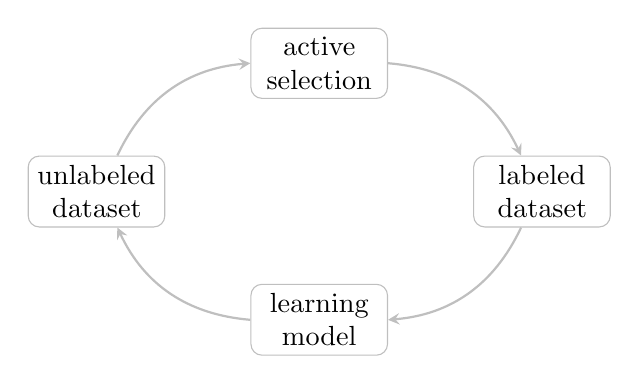
\begin{tikzpicture} [node distance = 4cm, on grid, auto]
 
\node (q0) [draw,lightgray, rounded corners, text width=1.5cm,yshift=-1.2cm, align =center] {\textcolor{black}{unlabeled \\dataset}};
\node (q1) [draw,lightgray, text width=1.5cm, rounded corners,above right = of q0,  yshift=-1.2cm,align =center] {\textcolor{black}{active \\selection}};
\node (q2) [draw,lightgray,rounded corners, text width=1.5cm, below right = of q1,yshift=1.2cm,align =center] {\textcolor{black}{labeled \\dataset}};
\node (q3) [draw,lightgray,rounded corners, text width=1.5cm, below left = of q2,yshift=1.2cm,align =center] {\textcolor{black}{learning \\model}};
 
\path [-stealth, thick]
    (q0) edge [lightgray, bend left]  (q1)
    (q1) edge [lightgray,bend left]  (q2)
    (q3) edge [lightgray,bend left]  (q0)
    (q2) edge [lightgray,bend left]  (q3);
\end{tikzpicture}
\caption{Active learning core structure. At each iteration a novel point is actively selected from the unlabeled set of data and the corresponding label is requested. Based on the received information, the model is modified.} \label{al}
\end{figure}

Indeed AL represents a training approach particularly suitable when labeled samples are too expensive or difficult to obtain. Specifically, AL is a particular ML algorithm based on a key idea: despite the shortage of labeled data, high accuracy results may be obtained if the training algorithm is allowed to choose the points to be labeled and learn from them \cite{settles1995active}. An AL algorithm asks an oracle to label the data considered most informative with an iterative approach. Doing so, since the queried points are directly selected by the learning algorithm, the amount of necessary labeled data is much smaller than that required for classical supervised ML approach. Figure \ref{al} shows the core structure of any AL algorithm: at each iteration the model is updated using the labelled dataset, and is allowed to ask for a new label in the unlabelled dataset. This process repeats until the model reaches sufficient performances or when the number of iterations reaches the maximum budget.

%\\In recent years, some active learning-based anomaly detection algorithms have been proposed.
%The idea of incorporating expert feedback in unsupervised anomaly detection algorithms aims at improving the achieved performance adding a relatively small computational cost. Active anomaly detection (AAD) algorithm \cite{das2016incorporating, das2017incorporating} proposes an active learning anomaly detection approach where points are ranked based on their anomalous behavior. The main goal is to maximize the number of true anomalies presented to the domain expert. An inclusion of AAD algorithm in the One Class Support Vector Machine (OCSVM) framework is tackled in \cite{lesouple2021incorporating}.
%Always using OCSVM, an expert feedback inclusion has been recently proposed %\cite{lesouple2021introduce}: to solve the problem, the paper combines together the $\mu$-SVM for the %labeled data and the OCSVM for the unlabeled set of data.

This paper focuses on the Isolation Forest detector, and suggests a strategy to tune it towards the user definition of anomaly. In this work the authors compare two AL query policies to ask the user new labels, and other two policies to update the internal structure with minimal computational effort. The goal is to increase the performance of the detector as much as possible, keeping very low both the labelling effort and the updating procedure. Moreover this method has two key advantages over the supervised and computationally expensive models: as it relies on an initial unsupervised training, it can start to work when there are no labels, but more importantly it can work even if instances from only one class are labelled. This is particularly useful when obtaining labels from the anomalous class is very uncommon or expensive.

%\gas{The rest of the papers is organized as follows: ...}
The rest of the paper is organized as follows. Initially, in Section \ref{rw} we outline the Isolation Forest in detail, and we indicate an existing active learning-based anomaly detection algorithm that will be used as a benchmark in thos work. Then, in Section \ref{pm} we illustrate the proposed model \approach: namely, we describe the strategies suggested to query the points as well as the approaches employed to update the model. In Section \ref{exp} we test \approach, comparing it with other models in relation to multiple real set of data. Finally, in Section \ref{conclusions} we draw conclusions for the present work.

%This paper compares two AL query strategies for anomaly detection using Isolation Forest. The algorithm key idea is to modify the internal structure of the unsupervised model based on a small amount of labeled data queried to the domain expert, trying to minimize the labelling effort but at the same time maximising the detection performance. Specifically, the presented model is based on the Isolation Forest model, i.e., the basic concept used to classify anomalies remains isolating data points from the rest of the dataset. Anyway, an innovative approach is used to query the labels and to update the model: novel information is achieved with the use of an active learning strategy by which the inner framework of the model is modified in order to match with the information obtained. Once the information is achieved, a user friendly iterative process allows to adapt the model by adjusting its structure on the basis of the novel input.
%The proposed method relies onto two distinguished yet essential issues: a process to select the most significant points and a tuning procedure to modify the structure of the model based on the information achieved. 
%This method has two key advantages over the supervised computationally expensive models: it is extremely computationally efficient and works even if instances from only one class are labelled.
%Based on the treated framework and on the data in hand, active learning algorithms are characterized by many possible query strategies \cite{settles1995active}. In this way, based on the considered purpose, the suitable query strategy may be selected and the corresponding most informative point may be labeled. 
%In the same way, we propose two possible approaches to address the selection of points to be labeled, producing two different query strategies with respect to both their benefits as well as their computational costs.
%\tommi{bisognerebbe scrivere che testiamo il nostro metodo su dataset reali e pubblichiamo il codice bla bla bla.}
%The importance of the algorithm...
%As we will see later the proposed model is based on...
%Section \ref{} ecc..
%list of the notation - simboli usati fare tabella





%\tommi{monitoring unexpected behaviour?} is essential. 
 %Even if, to date, there is no clear or official definition, broadly speaking, an anomalous point, also known as anomaly or outlier, is defined \textit{as an observation that deviates so much from other observations as to arouse suspicion that it was generated by a different mechanism} \cite{hawkins1980identification}. In general, an anomaly is identified as a variation from the norm, a data being characterised by a different behaviour with respect to other data that distinguishes itself from the rest of the dataset. Consequently, anomaly detection algorithms aim at detecting or identifying data that seem not to conduct themselves with a standard trend.
%\tommi{non sembra che parliamo di distribuzione gaussiana?}. 
%Anomaly detection techniques may be divided into three groups based on the available data in use: supervised, unsupervised and semi-supervised. 
%If the dataset contains labeled data, any technique for binary classification may be used, leading to highly accurate results. 
%Unfortunately, a critical challenge of anomaly detection is the lack of labeled data \cite{chandola2009anomaly}. Obtaining labels requires an often too expensive cost to take care of, since the labeling procedure is usually carried on by a human expert domain who, by hand labels each point with a time consuming and demanding routine. To solve this matter, semi-supervised or unsupervised techniques are employed. In the first scenario, a labeled portion of the original dataset is required, usually belonging to the most representative normal class, and, based on such labeled data, a model representing the normal behaviour is produced. \tommi{dici?} Generally, in fact, labeling normal data requires less efforts: normal points tend to have a common and more static behavior, making it easier to  be identified.
%For the classical unsupervised anomaly detection problem, the purpose is to isolate outliers with no use of labeled data based on the fact that normal data greatly outnumbers anomalous data. As a rule, unsupervised anomaly detection models are not tuned for the precise domain of application but are generally based on identifying rules based on specific data characteristics. 
%Based on the context and on the problem in question, different popular anomaly detection techniques exist. 
%\tommi{tornarci} A large class of unsupervised anomaly detectors are those based on statistical methods. These techniques produce a statistical distribution based on the given set of data and classify points according to where data falls: points that are not consistent or that simply lie in the tails of the computed distribution are consider anomalies \cite{hochenbaum2017automatic, hill2010anomaly}. 
%Some anomaly detection methods are based on the traditional classification problem. Based on the classical Support Vector Machine framework several methods have been proposed: the one-class support vector machine \cite{scholkopf1999support} computes an hyperplane that separates the data points from the origin and at the same time maximizes its distance with respect to the origin; the support vector data description \cite{tax2004support} looks for the smallest hypersphere containing the considered dataset. Distance-based \cite{knorr1998algorithms} and density-based \cite{breunig2000lof} outlier detection methods try to solve the problem by finding a profile for normal data based on inner data characteristics: the first uses the average distance of points, since, by nature, outliers have a higher value with respect to normal points; the latter is based on density area, due to the fact that outliers tend to stay in low density areas compared to normal points, which usually assemble in the same area. 

% tommi: andrei a capo in modo da evidenziare IF che è il metodo che andremmo ad analizzare
%A very popular anomaly detection algorithm is the Isolation Forest algorithm \cite{liu2008isolation, liu2012isolation}, which presents a brand-new approach: instead of creating a profile for normal data, it explicitly tries to isolate anomalies. To do it, Isolation Forest relies on two anomaly inner characteristics: they are fewer in number and they have very different attributes compared to normal data. 

%To cope with the lack of labeled data, in recent years some active learning-based anomaly detection algorithms have been proposed.
%The idea of incorporating expert feedback in unsupervised anomaly detection algorithms aims at improving the achieved performance adding a relatively small computational cost. Active anomaly detection (AAD) algorithm \cite{das2016incorporating, das2017incorporating} propose an active learning anomaly detection approach where points are ranked based on their anomalous behavior. The main goal is to maximize the number of true anomalies presented to the domain expert. An inclusion of AAD algorithm in the One Class Support Vector Machine (OCSVM) framework is tackled in \cite{lesouple2021incorporating}.
%Always using OCSVM, an expert feedback inclusion has been recently proposed \cite{lesouple2021introduce}. To solve the problem, the paper combines together the $\mu$-SVM for the labeled data and the OCSVM for the unlabeled set of data. 
%\cite{vercruyssen2018semi}. 


%This paper presents a novel active learning strategy for anomaly detection using Isolation Forest. The algorithm key idea is to modify the internal structure of the unsupervised model based on a small amount of labeled data queried to the domain expert, trying to minimize the labelling effort but maximising the detection performance. Specifically, the presented model is based on the Isolation Forest model, i.e., the basic concept used to classify anomalies remains isolating data points from the rest of the dataset. Anyway, an innovative approach is used to query the labels and to update the model: novel information is achieved with the use of an active learning strategy by which the inner framework of the model is modified in order to match with the information obtained. Once the information is achieved, a user friendly iterative process allows to adapt the model by adjusting its structure on the basis of the novel input.
%Based on the treated framework and on the data in hand, active learning algorithms are characterized by many possible query strategies \cite{settles1995active}. In this way, based on the considered purpose, the suitable query strategy may be selected and the corresponding most informative point may be labeled. 
%In the same way, we propose two possible approaches to address the selection of points to be labeled, producing two different query strategies with respect to both their benefits as well as their computational costs.
%\tommi{bisognerebbe scrivere che testiamo il nostro metodo su dataset reali e pubblichiamo il codice bla bla bla.}
%The importance of the algorithm...
%As we will see later the proposed model is based on...
%Section \ref{} ecc..
%list of the notation - simboli usati fare tabella

%
% vars
%
\newcommand{\X}{\ensuremath{\mathbf{X}}}
\newcommand{\B}{\ensuremath{\mathbf{B}}}
\newcommand{\Y}{\ensuremath{\mathbf{Y}}}
\newcommand{\Z}{\ensuremath{\mathbf{Z}}}
\newcommand{\Q}{\ensuremath{\mathbf{Q}}}
\newcommand{\Cb}{\ensuremath{\mathbf{C}}}
\newcommand{\V}{\ensuremath{\mathbf{V}}}
\newcommand{\A}{\ensuremath{\mathbf{A}}}
\newcommand{\x}{\ensuremath{\boldsymbol{x}}}
\newcommand{\bo}{\ensuremath{\boldsymbol{b}}}
\newcommand{\y}{\ensuremath{\boldsymbol{y}}}
\newcommand{\z}{\ensuremath{\boldsymbol{z}}}
\newcommand{\e}{\ensuremath{\boldsymbol{e}}}
\newcommand{\PC}{\ensuremath{\mathcal{C}}}
\newcommand{\PCaug}{\ensuremath{\mathcal{A}}}
\newcommand{\LC}{\ensuremath{\mathcal{L}}}
\newcommand{\WMCC}{\ensuremath{\mathcal{C}}}
\newcommand{\PSDD}{\ensuremath{\mathcal{C}}}
\newcommand{\AOMDD}{\ensuremath{\mathcal{C}}}
\newcommand{\PDG}{\ensuremath{\mathcal{C}}}
\newcommand{\primep}{\ensuremath{\mathsf{P}}}
\newcommand{\sub}{\ensuremath{\mathsf{S}}}
\newcommand{\CNET}{\ensuremath{\mathcal{C}}}
\newcommand{\C}{\ensuremath{\mathcal{C}}}
\newcommand{\CLT}{\ensuremath{\mathcal{T}}}
\newcommand{\model}{\ensuremath{\mathsf{m}}}
\newcommand{\modelfam}{\ensuremath{\mathcal{M}}}
\newcommand{\val}{\ensuremath{\mathsf{val}}}
\newcommand{\supp}{\ensuremath{\mathsf{supp}}}
\newcommand{\structure}{\ensuremath{\mathcal{G}}}
\newcommand{\tree}{\ensuremath{\mathcal{T}}}
\newcommand{\graph}{\ensuremath{\mathcal{G}}}
\newcommand{\params}{\ensuremath{\boldsymbol{\theta}}}
\newcommand{\sumparams}{\ensuremath{\boldsymbol{\theta}_{\mathsf{S}}}}
% \newcommand{\sumparams}{\ensuremath{\boldsymbol{\omega}}}
\newcommand{\leafparams}{\ensuremath{\boldsymbol{\theta}_{\mathsf{L}}}}
%\newcommand{\leafparams}{\ensuremath{\boldsymbol{\lambda}}}
\newcommand{\scope}{\ensuremath{{\phi}}}
\newcommand{\mixture}{\ensuremath{\mathcal{M}}}
\newcommand{\vtree}{\ensuremath{\mathcal{V}}}
% \newcommand{\p}{\ensuremath{\mathsf{Pr}}}
\newcommand{\p}{{p}}
\newcommand{\q}{{q}}
\newcommand{\m}{{m}}
\newcommand{\ch}{\ensuremath{\mathsf{in}}}
\newcommand{\pa}{\ensuremath{\mathsf{pa}}}
\newcommand{\leftn}{\ensuremath{\mathsf{L}}}
\newcommand{\rightn}{\ensuremath{\mathsf{R}}}% \newcommand{\f}{\ensuremath{f}}
\newcommand{\f}{\ensuremath{\Delta}}
\newcommand{\vtreenode}{\ensuremath{\mathcal{v}}}
\newcommand{\Ent}{\ensuremath{\mathbb{H}}}
\newcommand{\Mom}{\ensuremath{\mathbb{M}}}
\newcommand{\Ex}{\ensuremath{\mathbb{E}}}
\newcommand{\interval}{\ensuremath{\mathcal{I}}}
\newcommand{\Le}{\ensuremath{\mathsf{L}}}
\newcommand{\Ri}{\ensuremath{\mathsf{R}}}

\newcommand{\poly}[1]{\texttt{poly}(#1)}

%
% misc, writing
%
\newcommand{\eg}{e.g.,\ }
\newcommand{\wrt}{w.r.t.\ }
\newcommand{\ie}{i.e.,\ }
\newcommand{\cf}{cf.\ }
\newcommand{\aka}{a.k.a.\ }
\newcommand{\iid}{i.i.d.\ }

%
% symbols, concepts
\newcommand{\prob}{\ensuremath{\mathsf{Pr}}}
\newcommand{\uprob}{\ensuremath{{\bwidetilde{\mathsf{P}}\mathsf{r}}}}

%
% operators
\newcommand{\vars}{\ensuremath{\mathsf{vars}}}
\newcommand{\id}[1]{\llbracket{#1}\rrbracket}
\newcommand{\neigh}{\ensuremath{\mathsf{neigh}}}

\newcommand{\mathL}{\mathcal{L}}
\newcommand{\mathP}{\mathcal{P}}
% \newcommand{\E}{\mathcal{E}}
\newcommand{\data}{\mathcal{D}}
\newcommand{\F}{\mathcal{F}}
\newcommand{\mi}{\text{MI}}
\newcommand{\true}[0]{\texttt{true}}
\newcommand{\false}[0]{\texttt{false}}
\newcommand{\oplusl}{\operatornamewithlimits{\oplus}}
\newcommand{\otimesl}{\operatornamewithlimits{\otimes}}
\newcommand{\landl}{\operatornamewithlimits{\land}}

%
\newcommand{\flow}{\mathrm{F}}
\newcommand{\expflow}{\mathrm{EF}}
\newcommand{\context}{\gamma}
\newcommand{\pseudocount}{\alpha}
\newcommand{\bigO}{\mathcal{O}}
\newcommand{\bigOmega}{\Omega}
\newcommand{\bigTheta}{\Theta}
\newcommand{\indicator}[1]{\mathbbm{1}[#1]}
\newcommand{\weight}[2]{\mathtt{weight}(#1,#2)}
\newcommand{\entropy}{\mathtt{ENT}}
\newcommand{\expectation}{\mathbb{E}}
\newcommand{\LL}{\mathtt{LL}}
\newcommand{\lit}{\mathtt{Lit}}

\newcommand{\pluseq}{\mathrel{+}=}
\newcommand{\minuseq}{\mathrel{-}=}

\newcommand{\w}{\mathbf{w}}
\newcommand{\W}{\mathbf{W}}

\newcommand{\bp}{\mathbf{p}}

\newcommand{\SL}{\mathrm{L}^{\mathrm{s}}}
\newcommand{\WSL}{\mathrm{L}^{\mathrm{ws}}}
\newcommand{\MC}{\mathtt{MC}}

%
% queries
\newcommand{\nlquery}[2]{\begin{minipage}{.07\textwidth}$q_{#1}:$\end{minipage}\begin{minipage}{.88\textwidth}\raggedright\emph{#2}\end{minipage}}

\newcommand{\SPLIT}{\mathtt{SPLIT}}

\newcommand{\given}{\vert}
\section{Related work}
\label{sec:relatedwork}

We now discuss how our results relate to phenomena that have been observed or proven in the literature before.

\paragraph{Robust and non-robust useful features}
In the words of \citet{ilyas19, springer21}, for
directed attacks, all robust features become less useful, but adversarial
training uses robust features more.  In the small sample-size regime
$n<d-1$ in particular, robust learning assigns so much weight
on the robust (possibly non-useful) features, that the signal in the non-robust
features is drowned. This leads to an unavoidable and large increase
in standard error that dominates the decrease in susceptibility and
hence ultimately leads to an increase of the robust error.

\paragraph{Small sample size and robustness}
A direct consequence of Theorem~\ref{thm:linlinf} is that in order to
achieve the same robust error as standard training, adversarial
training requires more samples. This statement might remind the reader
of sample complexity results for robust generalization in
\citet{schmidt18, Yin19, Khim18}. While those results compare sample
complexity bounds for standard vs. robust error, our theorem
statement compares two algorithms, standard vs. adversarial training,
with respect to the robust error.


\paragraph{Trade-off between standard and robust error} 

Many papers observed that even though adversarial training decreases robust error compared to standard training, it may lead
to an increase in standard test error \cite{madry18, zhang19}.  
%This
%trade-off phenomenon has been theoretically studied under different
%assumptions: \cite{nakkiran19, madry18} show that small model capacity
%could result in the poor generalization performance. 
For example, \citet{tsipras19, zhang19, javanmard20, dobriban20, chen20} study settings where the Bayes optimal robust classifier is not equal to the Bayes optimal (standard)
classifier (i.e. the perturbations are inconsistent or the dataset is non-separable).
%% However, these settings inherently assume inconsistent3
%% $\ell_p$-ball perturbations, i.e. where perturbations may also change
%% the ground truth label.
%% By definition however, adversarial attacks
%% are “only useful” when they do not change the class for the ground
%% truth classifier such as the human (like for traffic sign stickers or
%% imperceptible perturbation).  Also, neural networks are known to be
%% complex enough to even fit random labels and inputs.
\cite{raghunathan20} study consistent perturbations, as in our paper,
and prove that for small sample size, fitting adversarial
examples can increase standard error even in the absence of
noise. In contrast to aforementioned works, which do not refute that
adversarial training decreases robust error, we prove that for
\nameofattacks perturbations, in the small sample regime adversarial training may also increase \emph{robust error}.

%As a reaction to the trade-off phenomenon,
\paragraph{Mitigation of the trade-off} 
A long line of work has proposed procedures to 
mitigate the trade-off phenomenon.  For example \citet{alayrac19,
  Carmon19, zhai20, raghunathan20} study robust self training, which
leverages a large set of unlabelled data, while \citet{lee20, lamb19,
  xu20} use data augmentation by interpolation. \citet{Ding20,
  balaji19, Cheng20} on the other hand propose to use adaptive
perturbation budgets $\epstrain$ that vary across inputs. 
%Their
%approach is closest to the story of this paper, although it is
%motivated by inconsistent perturbations. 
%Some of these mitigation approaches also result in an increase in robust accuracy against
%$\ell_p$-perturbations and hence might be candidates to successfully increase robust accuracy for \nameofattacks perturbations in the small sample size regime.
Our intuition from the theoretical analysis suggests that the standard
mitigation procedures for imperceptible perturbations may not work for
perceptible \nameofattacks, because all relevant features are non-robust.
%% robustness inherently requires
%% using the signal component in the data less. 
%% less weight on
%% the signal component in the data.
We leave a thorough empirical study
as interesting future work.

%\paragraph{Perceptible adversarial perturbations} \jc{doubting}
%% Multiple works have considered perceptible perturbations in the form of adversarial perceptible perturbations or common image corruptions. For example stickers on traffic signs \cite{Eykholt18}, adversarially coloured glasses or face-stickers \cite{Wu20} and adversarial watermarks \cite{Hayes18}. The common defences against these attacks are data-augmentation techniques such as adversarial training and variants thereof. 

 %adaptive perturbation budgets $\epstrain$ are proposed.
%% In many cases we observe that adversarial training, while gaining some robust accuracy, can cause a drop in clean test accuracy \cite{madry18, zhang19}. In \cite{tsipras19, zhang19} they advocate that the drop in standard accuracy stems from a general trade-off between the standard and robust accuracy objectives. In contrast, \cite{yang20} shows that there exist solutions in commonly used function spaces that achieve both objectives on common datasets. We show that adversarial training with signal-attacking perturbations can also hurt robust generalization. \jc{would need to get this in there aboout sample complexity} In \cite{schmidt18}, they show that finding robust classifiers may require more samples whereas in \cite{nakkiran19, madry18} they find that robustness may require a larger model capacity.

%% Recent work has tried to come up with different approaches to mitigate
%% the drop in standard accuracy. For example \cite{alayrac19, Carmon19, zhai20, raghunathan20} propose robust self training, which leverages unlabelled data, the works \cite{lee20, lamb19, xu20} use data augmentation by interpolation and in the works \cite{Ding20, balaji19, Cheng20} adaptive perturbation budgets $\epstrain$ are proposed. We expect the methods that are able to increase standard accuracy or fully mitigate the drop, to also help adversarial training in the small sample size regime. In particular, robust self-training may help, but is because of the large unlabelled data set recourse and time expensive. 
%% In \cite{ilyas19, springer21} they characterize the existence of robust useful features, useful features and non-useful features. Our work aligns with this perspective. In the low sample regime, adversarial training causes the classifier to rely heavier on non-useful features to classify the dataset. This in contrast to the high sample regime where adversarial training gains robust accuracy by causing the classifier to comparatively rely less on non-robust useful features instead then more on non-useful features. 

%% In \cite{bhattacharjee20} they note that adversarial training can hurt robust generalisation one sample at the time. We characterize the phenomenon and give statistical bounds. In \cite{Bornschein20, Brigato21} they consider deep learning in the low sample regime. Both works find that smaller models may outperform larger commonly used models in the low sample regime. Our results comply with the results published there, but we note the high dependence on the specific dataset.



%% \paragraph{Non-perfect adversarial training}
%% On the other hand, recent empirical and theoretical papers have noted that test
%% robust accuracy might decrease with robust training accuracy and hence regularizing model complexity could benefit robust generalization \cite{rice20, Sanyal20, Donhauser}, a phenomenon referred to as robust overfitting. 
%% \fy{whats this adversarial feature overfitting - are there other overfitting things}
%% \fy{dunno if that stuff on non-robust features is any relevant}

%% Here we have perfectly certified models and still have that it hurts.
%% \fy{certification is in some sense uber perfect fitting attack models - should be even worse than just interpolating on adversarial examples?}

%% Attack-model overfitting
%% We want to emphasize that usually

%% Recent work has tried to come up with different approaches to mitigate
%% the drop in standard accuracy 
%% some of which show final improvement in ....
%% We expect them to work well 

\section{A Closer Look at Non-linearity in Adam}
\label{sec:motivation}
\begin{figure*}[t!]
  \centering
  \subfigure[$\|\*v_t-\*v_{t-1}\|$]{
  \includegraphics[width=0.23\textwidth]{./sections/figure/v_diff.png}\label{fig:profile_bert_large:var_diff_time}}
  \subfigure[$\|\*v_t^{(0)}-\*v_t\|$]{
  \includegraphics[width=0.23\textwidth]{./sections/figure/v_diff_local.png}\label{fig:profile_bert_large:var_diff_local}}
  \subfigure[$\|\*m_t-\*m_{t-1}\|$]{
  \includegraphics[width=0.23\textwidth]{./sections/figure/m_diff.png}\label{fig:profile_bert_large:mom_diff_time}}
  \subfigure[$\|\*m_t^{(0)}-\*m_t\|$]{
  \includegraphics[width=0.23\textwidth]{./sections/figure/m_diff_local.png}\label{fig:profile_bert_large:mom_diff_local}}
  \caption{Momentum and variance Profiling for BERT-Large sequence 128 pretraining with original Adam using 64 GPUs. For variance, we profile two types of metrics: the first is the difference between local and global variance: $\|\*v_t^{(0)}-\*v_t\|$, where $\*v_t^{(0)}$ and $\*v_t$ denotes the variance term computed via local gradient on worker-0 and the gradient from full-precision AllReduce, respectively. We also profile the variance difference in adjacent step $\|\*v_t-\*v_{t-1}\|$. Similarly, we profile the same two metrics for the momentum.}
  \label{fig:profile_bert_large}
\end{figure*}

In this section, we provide a more formal description on the problem setting and illustrate the limitations from the original Adam and the state-of-the-art 1-bit Adam \citep{tang20211}.

\textbf{Problem Formulation.}
In this paper, we consider the following optimization problem:
\begin{align}
    \min_{\*x\in\mathbb{R}^d}f(\*x) = \mathbb{E}_{\zeta\sim\mathcal{D}}f(\*x;\zeta).
\end{align}
where $\*x$ denotes the $d$-dimensional model. $\mathcal{D}$ denotes the training set and $f(\*x;\zeta)$ is the loss incurred over sample $\zeta$ given model parameters $\*x$.
The structure of the problem naturally captures many of the model training problems.

\textbf{The non-linearity in Adam.}
At step $t\geq 0$, denote $\*x_t$ and $\*g_t$ as the model parameters and stochastic gradient computed at step $t$, respectively. The update formula of SGD and Adam\footnote{Note that in Adam, operations like division should act element-wise.} can be summarized as:
\begin{align}
\label{equa:SGD_update}
\text{SGD update: } & \*x_{t+1} \leftarrow \*x_t - \gamma \*g_t. \\
\text{Adam update: } & \*m_{t+1} \leftarrow \beta_1\*m_{t} + (1-\beta_1)\*g_t, \nonumber \\
& \*v_{t+1} \leftarrow \beta_2\*v_{t} + (1-\beta_2)(\*g_t)^2, \nonumber \\
    \label{equa:Adam_update}
    & \*x_{t+1} \leftarrow \*x_t - \underbrace{\frac{\gamma}{\sqrt{\*v_t + \epsilon}}}_{\text{effective learning rate}} \cdot \*m_t,
\end{align}
where $\gamma$ is the learning rate, $\epsilon$ is a small constant to prevent zero division, $\beta_1$ and $\beta_2$ are tunable decaying factors.
The linearity in SGD update implies when using compression or local steps, the potential noise from (accumulated) gradients is in the order of $O(\gamma)$, which approaches zero when learning rate is decaying or set to be small. By comparison, the two auxiliary optimizer states in Adam, momentum ($\*m$) and variance ($\*v$), introduce non-linearity in the model update. 

Equation~(\ref{equa:Adam_update}) gives the formula of Adam when running it sequentially. In a distributed setting with $n$ workers, $\*g_t$ in Equation~(\ref{equa:Adam_update}) is often computed in parallel on different workers. Mathematically, if we denote $\*g_t^{(i)}$ as the stochastic gradient computed on the $i$-th worker at step $t$, then distributed Adam can be written as replacing $\*g_t$ with $1/n\sum_{i=1}^n{\*g_t^{(i)}}$ in Equation~(\ref{equa:Adam_update}) as follows:
\begin{align*}
\*m_{t+1} \leftarrow \beta_1\*m_{t} + (1-\beta_1)\left(1/n\sum\nolimits_{i=1}^n{\*g_t^{(i)}}\right), \hspace{1mm} \*v_{t+1} \leftarrow \beta_2\*v_{t} + (1-\beta_2)\left(1/n\sum\nolimits_{i=1}^n{\*g_t^{(i)}}\right)^2.
\end{align*}
% This non-linearity brings up two limitations: 1) when aggressively compressing the gradient such as with 1-bit quantizer, all the coordinate-wise effect learning rate $\gamma/\sqrt{\*v_t+\epsilon}$ will become the same value, so that Adam no longer enjoys adaptive and fast convergence; 2) to keep all parallel workers to have a consensus on the optimizer state ($\*m$ and $\*v$), which is an important property for convergence, the existence of non-linearity forces all the workers to perform synchronization when performing local steps. However, this would add expensive synchronization overhead


\textbf{Issue with non-linearity on 1-bit  compression.}
The main bottleneck in running distributed Adam is the accumulation of $1/n\sum\nolimits_{i=1}^{n}\*g_t^{(i)}$ since the gradients are usually high-dimensional. 
Based on the profiling results from \citep{tang20211,li20211}, the communication of gradients could take up to 94\% of the total training time on modern clusters.
Gradient compression mitigates this issue by sending and averaging gradients with fewer bits. However, in Adam this causes the loss on the learning rate adaptivity. Consider using the aggressive
1-bit compression \citep{liu2018signsgd}, which sends each gradient with only signs and a shared, usually the average over all the coordinates, magnitude. More specifically, denote $\mathcal{C}[\cdot]$ as the 1-bit compression, then
\begin{align}
\label{equa:1bitcompression}
    \mathcal{C}[\*a] = \frac{\|\*a\|_1}{d} \cdot \text{sign}(\*a), \forall \*a\in\mathbb{R}^d.
\end{align}
It is straightforward to observe that naively applying 1 bit to compress gradients in the original Adam loses coordinate-wise adaptivity since sharing magnitude makes all the coordinates-wise learning rate $\gamma/\sqrt{\*v_t+\epsilon}$ the same value. This makes Adam no difference than momentum SGD.

\textbf{Issue with non-linearity on local steps.}
In SGD (Equation~(\ref{equa:SGD_update})), the model updates are linearly dependent on the gradients and has zero additional states. It implies with local steps, the parallel workers can entirely reach consensus after a single round of synchronization, even with compression \citep{basu2020qsparse}. However, in Adam simply synchronizing the model can still leave the momentum and variance out-of-sync. This makes parallel workers fail to capture the global adaptivity when the system scales up.
To give a more concrete example, we profile a full run of BERT-Large pre-training with original Adam, and summarize different metrics of momentum and variance in Figure~\ref{fig:profile_bert_large}. As shown in Figure~\ref{fig:profile_bert_large:mom_diff_local} and \ref{fig:profile_bert_large:var_diff_local}, the difference between local and global optimizer states, momentum and variance, remain constants and do not decrease to zero.

\textbf{1-bit Adam and its limitations.}
1-bit Adam \citep{tang20211} is a state-of-the-art solution that addresses non-linearity in 1-bit compression. 1-bit Adam adopts a pre-conditioned variance state from running original Adam for $T_0$ steps first. 
% Note that here we defer the details of 1-bit compression to Appendix~\ref{appendix:sec:algorithm} and treat it as a black-box procedure named \textbf{1bit-AllReduce} while the original full-precision AllReduce is referred to as \textbf{AllReduce}. 
The intuition there is that at later stage of training, the variance state becomes stable so that $\*v_{T_0}$ can be a good approximation of variance state for the remaining steps. 
As paritally illustrated in Section~\ref{sec:intro}, the full-precision stage of 1-bit Adam still presents non-trivial overhead. For instance: as illustrated in \citep{tang20211}, when training BERT-Large on 64 GPUs using Ethernet, while the full-precision stage contains 15\% of the total steps, it can take more than 50\% of the entire training in terms of the wall-clock time\footnote{Concretely, it shows in \citep{tang20211} Section 7.1 that to train BERT-Large on 64 GPUs using Ethernet, the full-precision Adam takes 174.3 hours in total while 1-bit Adam takes 51.5 hours. By a simple calculation, we know that full-precision stage of 1-bit Adam takes approximately 26.37 hours while the compression stage takes 25.13 hours.}.
Additionally, 1-bit Adam is restricted in the scope of compression, how it handles other techniques such as local steps remains open question.
% Additionally, we profile the per-step time for BERT-Large pretraining on a Ethernet cluster\footnote{The detailed profiling numbers can be found in Appendix~\ref{appendix:sec:experiment}.} and observe in a single step, the fixed cost of communication can take up to 4$\times$ of the computation time. This implies when data volume per-parameter reaches its extreme in training large models at large scales, the fixed cost of communication and compression could gradually become the bottleneck that dominates the computation time.


\section{Full Description to AllReduce}
\label{appendix:sec:algorithm}

As introduced in Section~\ref{sec:related work}, the error feedback based \textbf{1bit-AllReduce} works best both in theory and in practice. In fact, the original 1-bit Adam also adopts the error-feedback design \citep{tang20211}. We give the full description of this \textbf{1bit-AllReduce} in Algorithm~\ref{algo:EF}, to replace the \textbf{1bit-AllReduce} in Algorithm~\ref{algo:localstep01}. In the theoretical analysis, our proofs will also rely on this algorithm. Note that this algorithm does not require any additional assumptions for our theory to hold, since this fits the black-box procedure in Algorithm~\ref{algo:basic01} and Algorithm~\ref{algo:localstep01}.

\begin{algorithm}[ht!]
	\caption{The full description of Error Feedback 1 bit Communication (\textbf{1bit-AllReduce})}\label{algo:EF}
	\begin{algorithmic}[1]
		\Require communication buffer $\*z_{t}^{(i)}$, worker error $\*\delta_{t}^{(i)}$, server error $\overline{\*\delta}_{t}$, 1-bit compressor $\mathcal{C}[\cdot]$. Both worker and server errors will be initialized at $\*0$ at $t=0$.
	    \State \textbf{(On $i$-th node)}
	    \State Compress $\*z^{(i)}_{t}$ into $\hat{\*z}^{(i)}_{t}=\mathcal{C}[\*z^{(i)}_{t}+\*\delta^{(i)}_{t}]$, and update the compression error by $\*\delta^{(i)}_{t+1} = \*z^{(i)}_{t}+\*\delta^{(i)}_{t} - \hat{\*z}^{(i)}_{t}$.
	    \State Send $\hat{\*z}^{(i)}_{t}$ to the server.
	    \State \textbf{(On server)}
	    \State Take the average over all the $\hat{\*z}^{(i)}_{t}$ and compress it into $\overline{\*z}_{t} = \mathcal{C}[\frac{1}{n}\sum_{i=1}^{n}\hat{\*z}^{(i)}_{t+1} + \overline{\*\delta}_{t}]$, and update the compression error by $\overline{\*\delta}_{t+1} = \frac{1}{n}\sum_{i=1}^{n}\hat{\*z}^{(i)}_{t} + \overline{\*\delta}_{t} - \overline{\*z}_{t}$.
	    \State Send $\overline{\*z}_{t}$ to all the workers.
	    \State \textbf{(On $i$-th node)}
		\State \textbf{return} $\overline{\*z}_{t}$, $\*\delta_{t+1}^{(i)}$, $\overline{\*\delta}_{t+1}$.
	\end{algorithmic}
\end{algorithm}

\begin{algorithm}[ht!]
	\caption{The full description of \textbf{AllReduce}}\label{algo:AllReduce}
	\begin{algorithmic}[1]
		\Require communication buffer $\*z_{t}^{(i)}$.
	    \State \textbf{(On $i$-th node)}
	    \State Send $\*z^{(i)}_{t}$ to the server.
	    \State \textbf{(On server)}
	    \State Take the average over all the ${\*z}^{(i)}_{t}$ into $\overline{\*z}_{t} = \frac{1}{n}\sum_{i=1}^{n}{\*z}^{(i)}_{t}$.
	    \State Send $\overline{\*z}_{t}$ to all the workers.
	    \State \textbf{(On $i$-th node)}
		\State \textbf{return} $\overline{\*z}_{t}$.
	\end{algorithmic}
\end{algorithm}
\section{Convergence Analysis}
\label{sec:theory}
In this section, we provide the convergence guarantee for %Algorithm~\ref{algo:basic01} under arbitrary freezing policy and 
{\myalgo} (Algorithm~\ref{algo:localstep01}) under arbitrary freezing policy $\mathcal{T}_{\*v}$ and local steps policy $\mathcal{T}_{\*u}$. In the main paper, we provides the convergence rate in the general case. However, different $\mathcal{T}_{\*v}$ or $\mathcal{T}_{\*u}$ gives us the opportunity to obtain tighter bounds. We leave these discussion in the appendix.
We start by making the following assumptions.

\begin{assumption}
\label{assum:smooth}
\textbf{Lipschitzian gradient:} $f(\cdot)$ is assumed to be  with $L$-Lipschitzian gradients, which means $\quad \|\nabla f(\*{x}) - \nabla f(\*{y}) \| \leq L \|\*{x} - \*{y} \|, \forall \*{x},\forall \*{y}$.
\end{assumption}

\begin{assumption}
\label{assume:variance}
\textbf{Bounded variance:}
The stochastic gradient computed on each worker is unbiased and has bounded variance:$\mathbb E_{\zeta\sim\mathcal{D}}\|\nabla f(\*{x};\zeta) - \nabla f(\*{x})\|^2 \leq \sigma^2,\quad\forall \*{x}$.
\end{assumption}

\begin{assumption}
\label{assume:g_bound}
\textbf{Bounded gradient:}
    The infinity norm of stochastic gradient is bounded by a constant $G_\infty>0$ such that $\left\| \*g_t\right\|_\infty \leq G_\infty, \forall t$.
\end{assumption}

\begin{assumption}
\label{assume:local:compression}
\textbf{Compression error in Algorithm~\ref{algo:localstep01}:} For arbitrary $\*x\in\mathbb{R}^d$, there exists a constant $\Delta$, such that the output of compressor $\mathcal{C}[\cdot]$ has the following error bound: $\mathbb{E}\left\| \mathcal{C}[\*x] - \*x \right\|^2 \leq \Delta^2$.
\end{assumption}

\begin{assumption}
\label{assume:localstep_bound}
Given ordered set $\mathcal{T}_{\*u}$, denote $t_j$ as the $j$-th element in $\mathcal{T}_{\*u}$, we assume there exists a constant $H\geq 0$, it holds that $\max_{1\leq j<|\mathcal{T}_{\*u}|}(t_{j+1} - t_j)\leq H$.
\end{assumption}

\textbf{Remarks on the assumptions.}
Assumption~\ref{assum:smooth}, \ref{assume:variance} and \ref{assume:g_bound} are standard in the domain of non-convex optimization.
% and Assumption~\ref{assume:compression} is also commonly used in compression-based optimization \citep{alistarh2017qsgd}. 
Comparing with the 1-bit Adam paper \citep{tang20211}, we do not explicitly assume the uniform lower bound on the variance coordinate, i.e., $\*e_j^\top\*v>v_{\min}>0, \forall j$ for some constant $v_{\min}$. Instead we assume an infinity-norm bound on the gradient as in Assumption~\ref{assume:g_bound} which is more realistic. Assumption~\ref{assume:local:compression} is also assumed in \citep{tang20211}, in the appendix we discuss the variant of {\myalgo} that converges with weaker condition on the $\mathcal{C}$.

% We first give the convergence theorem for Algorithm~\ref{algo:basic01} as follows:
% \begin{theorem}
% \label{thm:basic01}
% Under Assumption~\ref{assum:smooth} to \ref{assume:g_bound}, let $m=|\mathcal{T}_{\*v}|$, 
% if we run Algorithm~\ref{algo:basic01} with a constant learning rate: for all $t\geq 0$
% \begin{align*}
%     \gamma_t = \left(\sigma\sqrt{\frac{T}{n}} + \frac{\beta_2^m}{2V_1L\sqrt{G_\infty^2+\epsilon}} + \frac{1}{125} \right)^{-1},
% \end{align*}
% then it holds that
% \begin{align*}
%     \frac{1}{T}\sum_{t=0}^{T-1} \mathbb{E}\|\nabla f(\*x_t)\|^2 \leq O\left( \frac{\beta_2^{-\frac{m}{2}}}{\sqrt{nT}} + \frac{(m+n)\beta_2^{-m}}{(1-\omega)^4T} +\frac{1}{T}\right),
% \end{align*}
% where we omit $f(\*0)-\inf_{\*x\in\mathbb{R}^d}f(\*x)$,  $G_\infty$, $d$, $\epsilon$, $\sigma$, $\beta_1$ and $L$ as constants.
% \end{theorem}

% As will be showing in Section~\ref{sec:experiment}, in practice we usually set $m\ll T$, and considering that $\beta_2$ is close to 1 (e.g. its default value is 0.999), $m$ and $\beta_2^{-m}$ scales as constants compared to $T$. Therefore, the complexity bound suggests that Algorithm~\ref{algo:basic01} achieves the linear speed up, at rate $O\left(1/\sqrt{nT}\right)$, with respect to $n$ and $T$.
% In the literature, previous works like \citet{zaheer2018adaptive,defossez2020simple} indicate the original Adam would converge to a noise ball under constant learning rate. By comparison, Theorem~\ref{thm:basic01} guarantees Algorithm~\ref{algo:basic01} converges to a stationary point with arbitrary precision.

% To prove the convergence for Algorithm~\ref{algo:localstep01}, we drop Assumption~\ref{assume:compression} and instead adopt the following slightly stronger assumption.

% While this assumption may be strong for all step $t$, in practice (as will be shown in Section~\ref{sec:experiment}) we generally apply and increase the local steps in later part of the training, where the magnitude of momentum or model difference becomes stable. Note that this is also the assumption adopted by
% \citep{tang20211,tang2019doublesqueeze}.
The convergence for Algorithm~\ref{algo:localstep01} is then given in the follow theorem.
\begin{restatable}{thm}{thmzerooneadam}
\label{thm:local01}
Under Assumption~\ref{assum:smooth} to \ref{assume:localstep_bound}, let $m=|\mathcal{T}_{\*v}|$, select $\beta_1,\beta_2\in[0,1)$ that fulfills $m\leq \log(1-\beta_1)/\log(\beta_2)$,
if we run Algorithm~\ref{algo:localstep01} with a constant learning rate: for all $t\geq 0$
\begin{align*}
    \gamma_t = \min\left\{ \sqrt{\frac{n}{\sigma^2T}}, \frac{1}{4L\sqrt{G_\infty^2+\epsilon}},  \frac{2\sqrt{G_\infty^2+\epsilon}}{L},  \frac{1}{6} \right\},
\end{align*}
then it holds that
\begin{align*}
    \frac{1}{T}\sum_{t=0}^{T-1} & \mathbb{E}\|\nabla f(\tilde{\*x}_t)\|^2 \leq O\left( \frac{\sigma}{\sqrt{nT}} + \frac{H^2\Delta^2(m+n)}{T} +\frac{1}{T}\right),
\end{align*}
where $\tilde{\*x}_t=1/n\sum_{i=1}^{n}{\*x}_t^{(i)}$ and we omit $f(\*0)-\inf_{\*x\in\mathbb{R}^d}f(\*x)$, $G_\infty$, $d$, $\epsilon$, $\beta_1$, $\beta_2$ and $L$ as constants.
\end{restatable}

Theorem~\ref{thm:local01} shows that {\myalgo} Algorithm~\ref{algo:localstep01} essentially admits
the same convergence rate as distributed SGD in the sense that it achieves linear speed up, at rate $1/O(\sqrt{nT})$. The effect of compression ($\Delta$) and local steps ($H$) only appears on a non-dominating term.
% \vspace*{-2mm}

\section{Experiments}
\label{sec: exp}
% \vspace*{-1mm}


% In this section, we present our experiment results on how model sparsity simplifies {\MU}, \textit{i.e.}, reducing the performance gap  between approximate unlearning and   {\retrain}.
%across different data-model setups,   unlearning scenarios, and evaluation metrics.

%In this section, we begin by introducing some essential experiment setups, and then empirically show the relationship between sparsity and MU across multiple datasets, various model architectures, diverse machine unlearning methods, and different MU settings. Compared to the `prune first, then unlearn' paradigm, we find that sparsity-aware MU can further boost the benefits of sparsity. Finally, we extend our methods to trojan model cleanse application to demonstrate the effectiveness of our methods further.  
%\SL{[A short paragraph to summarize the experiment section]} 


\subsection{Experiment setups}
\label{sec: exp_setup}
%\vspace*{-1mm}

\noindent \textbf{Datasets and models.}
Unless specified otherwise, our experiments will focus  on image classification under 
 CIFAR-10 \cite{krizhevsky2009learning}  using ResNet-18 \cite{he2016deep}. Yet,  
 experiments  on 
  additional datasets (CIFAR-100 \cite{krizhevsky2009learning}, SVHN \cite{netzer2011reading}, and ImageNet \cite{deng2009imagenet}) and an  alternative model architecture (VGG-16 \cite{simonyan2014very}) can  be found in Appendix\,\ref{appendix: additional results}.
  Across all the aforementioned datasets and model architectures, our experiments consistently show that model sparsification can effectively reduce the gap between approximate unlearning and exact unlearning. 
  %-\ref{appendix: additional results}
 
 % Additional datasets, such as CIFAR-100 \cite{krizhevsky2009learning}, SVHN \cite{netzer2011reading}, and ImageNet \cite{deng2009imagenet} will be  presented in the Appendix\,\ref{appendix: additional results}.  
 
 % Moreover, Appendix\,\ref{appendix: additional results} showcases the results of an alternative model architecture, namely VGG-16 \cite{simonyan2014very}, on CIFAR-10 alongside ResNet-18. 
% We will consider imagery    {datasets}     including CIFAR-10 \cite{krizhevsky2009learning}, CIFAR-100 \cite{krizhevsky2009learning}, SVHN \cite{netzer2011reading}, and ImageNet \cite{deng2009imagenet}. ResNet-18 \cite{he2016deep} or VGG-16 \cite{simonyan2014very} will give the corresponding image classifier.
% We default use CIFAR-10 as the dataset and ResNet-18 as the model architecture. 
%the image classification model by default is   ResNet-18 \cite{he2016deep}. Yet, VGG-16 \cite{simonyan2014very} will also be used for evaluating unlearning performance across   architectures. 


% Following previous work in machine unlearning and pruning, we consider four datasets, including CIFAR-10 \cite{krizhevsky2009learning}, CIFAR-100 \cite{krizhevsky2009learning}, SVHN \cite{netzer2011reading} and Tiny-ImageNet \cite{le2015tiny}, and two architecture types including ResNet-18 \cite{he2016deep} and VGG-16 \cite{simonyan2014very}. More datasets, model configurations, and setups are summarized in Table \ref{}. 

%\paragraph{{\MU} baselines and implementations.}


\noindent \textbf{Unlearning and pruning setups.}
% \SL{[Focus on implementation details of training methods in both 'prune first, then unlearn', and `sparsity-aware unlearning'. In the first category, you need to mention all implementation details of unlearning methods, and pruning methods. In the second category, you need to specify {\MUSparse} and {\MUAO}, etc.
% }
 %In our experiments, 
 We   focus on two unlearning scenarios mentioned in Sec.\,\ref{sec: primer_MU}, \textit{class-wise forgetting} and \textit{random data forgetting} ({$10\%$ of the whole training dataset} {together with 10 random trials}). 
 %Unless specified otherwise,  the class-wise forgetting will be the default setting.
 %that randomly removes a subset of data points from a single class. By default,  we will focus on the class-wise forgetting scenario. 
In the `\textit{prune first, then unlearn}' paradigm, we   focus on unlearning methods ({\FT}, {\GA}, {\FF},  and {\IU}) shown in Tab.\,\ref{tab: summary_MU_methods_metrics}
when applying to sparse models.
%including  fine-tuning (\FT),  gradient ascent (\GA),  Fisher forgetting (\FF), and   influence unlearning (\IU). 
We  implement these methods following their official repositories. However, it is worth noting that  the  implementation of {\FF} in \citet{golatkar2020eternal}
modifies the model architecture in class-wise forgetting, \textit{i.e.}, removes the  prediction head  of the class to be scrubbed. 
%As a result, it does not allow for unlearning random data points. 
By contrast, other   methods   keep the model architecture  intact during unlearning. 
Also, we choose {OMP} as the  default pruning method, 
as justified in Fig.\,\ref{fig: results_pruning_comparison}.
\iffalse 
If we relax such a condition for {\FF},  then the  unlearning performance would significantly degrade. Thus, even if it may lack fairness to compare  other methods with {\FF}, we cover the latter in class-wise forgetting for completeness. 
%Towards a fair comparison, we implement {\FF}  without modifying the model architecture. 
\fi
\iffalse
In the `\textit{sparsity-aware unlearning}' paradigm,  the sparsity-promoting regularization parameter $\gamma$  in   \eqref{eq: MUSparse} is set to   $\gamma = 5\times10^{-5}$ if it is given by a constant. This is found by a line search over $[10^{-5}, 10^{-1}]$ across   tradeoffs between testing accuracy and unlearning accuracy. 
\SL{We implement the linearly decaying scheduler by $\gamma_t = (1 - \frac{t}{T})\gamma$, where $t$ is the epoch index, and $T$ is the total number of  epochs. The linearly incr1easing scheduler is similarly given by $\gamma_t = \frac{t}{T} \gamma$ in Tab.\,\ref{tab: ablation_l1_scheduler}.}
\fi
\iffalse
\JH{In the `\textit{sparsity-aware unlearning}' paradigm,  the sparsity-promoting regularization parameter $\gamma$  in   \eqref{eq: MUSparse} is set to   $\gamma = 5\times10^{-5}$ if it is given by a constant, $\gamma=9\times10^{-5}$ for linear decaying scheduler, and $\gamma=1\times10^{-4}$ for linear increasing scheduler. They are found by a line search over $[10^{-5}, 10^{-1}]$ across  trade-offs between testing accuracy and unlearning accuracy. 
We implement the linearly decaying scheduler by $\gamma_t = (1 - \frac{t}{T})\gamma$, where $t$ is the epoch index, and $T$ is the total number of  epochs. The linearly increasing scheduler is similarly given by $\gamma_t = \frac{t}{T} \gamma$ in Tab.\,\ref{tab: ablation_l1_scheduler}.}
\JC{Need update @Jinghan}
\fi
In the `\textit{sparsity-aware unlearning}' paradigm, the sparsity-promoting regularization parameter $\gamma$ in \eqref{eq: MUSparse} is determined through the line search in the interval $[10^{-5}, 10^{-1}]$, with consideration for the trade-off between testing accuracy and unlearning accuracy. For all schedulers, $\gamma$ is set around to $5 \times 10^{-4}$. The linearly increasing and decaying schedulers are implemented as $\gamma_t = \frac{2t}{T} \gamma$ and $\gamma_t = (2 - \frac{2t}{T})\gamma$ respectively, where $t$ is the epoch index and $T$ is the total number of epochs. 
%as specified in Tab.\,\ref{tab: ablation_l1_scheduler}.
%}
% \JH{We employ a linear decay scheduler for $\gamma$, implemented as a function of epoch, denoted as $\gamma_t = (1 - \frac{t}{E})\gamma$. In this equation, $t$ represents the current epoch, $E$ stands for the total number of unlearning epochs, and $\gamma$ is the initial value.} \JC{@Jinghan add some description on scheduled parameters.}%Further, we implement {\MUAO} by choosing the pruning ratio $p\% = 20\%$ per iteration.
We refer readers to Appendix\,\ref{appendix: training and unlearning settings} for more details. 
%\JC{[Add further details to appendix]}

%following its recent benchmark in  \cite{ma2021sanity}. 

%As we have shown in Fig.\,\ref{fig: results_pruning_comparison}, OMP outperforms SynFlow \cite{tanaka2020pruning} in  generalization when the sparsity  increases.

%(\textit{e.g.},  $95\%$ sparsity in Fig.\,\ref{fig: results_pruning_comparison} \SL{[xxx]}). Meanwhile, OMP is more effective than IMP for {\MU} due to its  computation efficiency and less dependence on the training dataset. 


\iffalse 
In the `prune first, then unlearn' paradigm, we mainly focus on 3 SOTA pruning methods, \ding{172} SynFlow \cite{tanaka2020pruning}, \ding{173} OMP \cite{frankle2018lottery}, and \ding{174} IMP \cite{frankle2018lottery}, which follows the recent IMP benchmark's  \cite{ma2021sanity} setting. We chose four commonly used machine unlearning methods mentioned in section \ref{sec: primer_MU},  \ding{172} Fine-tuning (\FT), \ding{173} Gradient ascent (\GA), \ding{174} Fisher Forgetting (\FF), and \ding{175}  Influence Unlearning (\IU). We remark that {\FF} manually changes the last layer when forgetting the whole class. In other unlearning methods, we do not change the model architecture. For a fair comparison, we only conduct {\FF} on the CIFAR-10 dataset. Further experiments on {\FF} are listed in Appendix\ref{}. We choose OMP as our default pruning setting in the `prune first, then unlearn' experiment results and will focus on forgetting one class scenario. To make a fair comparison, we tune the hyperparameters carefully for {\IU} method at different sparsity levels. As for the `Sparsity-aware unlearning', we choose {\GA} and {\FT} these two methods to integrate with these proposed unlearning methods. We refer readers to Table \ref{} for more training and unlearning details, such as hyperparameters for unlearning methods and training epochs.
\fi 

\noindent \textbf{Evaluation metrics.}
We evaluate the unlearning performance following Tab.\,\ref{tab: summary_MU_methods_metrics}. 
Recall that {\UA}   and {\MIAF}   depict the \textit{efficacy} of {\MU}, {\RA}  reflects the \textit{fidelity} of {\MU}, and {\TA}   and {\RTE}  characterize the \textit{generalization ability} and the \textit{computation efficiency} of  an unlearning method. 
%It is worth noting that in the class-wise forgetting scenario, the class to be scrubbed will   be excluded in the testing dataset when evaluating {\TA} (testing accuracy). 
We implement MIA (membership inference attack) using the prediction confidence-based attack method \cite{song2019privacy,yeom2018privacy}, whose effectiveness has been justified in \citet{song2020systematic} compared to other   methods. We refer readers to Appendix\,\ref{appendix: metric settings} for more implementation details. {To more precisely gauge the proximity of each approximate {\MU} to {\retrain}, we introduce a metric termed `Disparity Average'. This metric quantifies the mean performance gap between each unlearning method and {\retrain} across all considered metrics. A lower value indicates closer performance to {\retrain}.}
%\SL{[variance, class-wise forgetting variance]}


% We remarked that test accuracy (\TA) is evaluated on the remaining classes in the test dataset in the unlearning one-class scenario. 

% As for MIA methods, we fulfill inference attacks based on prediction confidence \cite{song2019privacy,yeom2018privacy}, which effectiveness is demonstrated in the paper \cite{song2020systematic} compared to other MIA methods. T
% able \ref{} lists more details about our evaluation settings.  
% \SL{[you can refer to Table\,\ref{tab: summary_MU_methods_metrics} for unlearning baselines and metrics but include additional details. e.g. what is the specific MIA method used and why?]}


\subsection{Experiment results}
\label{sec: experiment_results}
\iffalse
\begin{table*}[htb]
\centering
\vspace*{1mm}
\caption{Performance overview of various MU methods  on dense and 95\%-sparse models considering different unlearning scenarios:
 class-wise forgetting, 
 and random data forgetting. The forgetting data of random data forgetting ratio is $10\%$ of the whole training dataset, 
 the sparse models are obtained using OMP \cite{ma2021sanity}, and the unlearning methods and evaluation metrics are summarized in Tab.\,\ref{tab: summary_MU_methods_metrics}. {Class-wise forgetting is conducted class-wise.}
The performance is reported in the form $a_{\pm b}$, with mean $a$ and standard deviation $b$ computed over $10$ independent trials. 
A performance gap  against \textcolor{blue}{{\retrain}} is provided 
in (\textcolor{blue}{$\bullet$}). Note that the better performance of approximate unlearning corresponds to the smaller performance gap with the gold-standard retrained model.
}
\label{tab: overall_performance}
% \vspace*{0.1in} % Requirements, do not delete.
% \vspace*{-1mm}
\resizebox{0.95\textwidth}{!}{
\begin{tabular}{c|cc|cc|cc|cc|c}
\toprule[1pt]
\midrule
  \multirow{2}{*}{\MU}& \multicolumn{2}{c|}{{\UA}} & \multicolumn{2}{c|}{{\MIAF}}& \multicolumn{2}{c|}{{\RA}} & \multicolumn{2}{c|}{{\TA}}&{\RTE}  \\ 
  & \multicolumn{1}{c|}{{\textsc{Dense}}}  & \multicolumn{1}{c|}{$\mathbf{95\%}$ \textbf{Sparsity}}
    & \multicolumn{1}{c|}{\textsc{Dense}}  & \multicolumn{1}{c|}{$\mathbf{95\%}$ \textbf{Sparsity}}
    & \multicolumn{1}{c|}{\textsc{Dense}}  & \multicolumn{1}{c|}{$\mathbf{95\%}$ \textbf{Sparsity}}
      & \multicolumn{1}{c|}{\textsc{Dense}}  & \multicolumn{1}{c|}{$\mathbf{95\%}$ \textbf{Sparsity}} & (min)
  \\
% \cline{3-10}

\midrule
\rowcolor{Gray}
\multicolumn{10}{c}{Class-wise forgetting} \\
\midrule
\retrain &\textcolor{blue}{$100.00_{\pm{0.00}}$}    & \textcolor{blue}{$100.00_{\pm{0.00}}$}
&\textcolor{blue}{$100.00_{\pm{0.00}}$}   & \textcolor{blue}{$100.00_{\pm{0.00}}$}
&\textcolor{blue}{$100.00_{\pm{0.00}}$}    & \textcolor{blue}{$99.99_{\pm{0.01}}$}
&\textcolor{blue}{$94.83_{\pm{0.11}}$}   & \textcolor{blue}{$91.80_{\pm{0.89}}$}
 &43.23\\
  \FT &$22.53_{\pm{8.16}}$ (\textcolor{blue}{$77.47$})&${73.64}_{\pm{9.46}}$  (\textcolor{blue}{${26.36}$})&$75.00_{\pm{14.68}}$ (\textcolor{blue}{${25.00}$})& ${83.02}_{\pm{16.33}}$ (\textcolor{blue}{${16.98}$}) 
  &$99.87_{\pm{0.04}}$ (\textcolor{blue}{$0.13$}) & ${99.87}_{\pm{0.05}}$ (\textcolor{blue}{${0.12}$})&$94.31_{\pm{0.19}}$ (\textcolor{blue}{$0.52$})
 &$94.32_{\pm{0.12}}$ (\textcolor{blue}{$2.52$})
&   2.52
  
  
  
  \\
 \GA &$93.08_{\pm{2.29}}$ (\textcolor{blue}{6.92}) &${98.09}_{\pm{1.11}}$ (\textcolor{blue}{${1.91}$})
& $94.03_{\pm{3.27}}$ (\textcolor{blue}{5.97})& ${97.74}_{\pm{2.24}}$ (\textcolor{blue}{${2.26}$})
& $92.60_{\pm{0.25}}$ (\textcolor{blue}{$7.40$})& $87.74_{\pm{0.27}}$ (\textcolor{blue}{$12.25$}) 
& $86.64_{\pm{0.28}}$ (\textcolor{blue}{$8.19$})& $82.58_{\pm{0.27}}$ (\textcolor{blue}{$9.22$}) 
&   0.33
 \\
  {\FF}  & $79.93_{\pm{8.92}}$ (\textcolor{blue}{$20.07$})& ${94.83}_{\pm{4.29}}$ (\textcolor{blue}{${5.17}$}) 
  & $100.00_{\pm{0.00}}$ (\textcolor{blue}{$0.00$})& ${100.00}_{\pm{0.00}}$ (\textcolor{blue}{$0.00$}) 
    & $99.45_{\pm{0.24}}$ (\textcolor{blue}{$0.55$})& ${99.48}_{\pm{0.33}}$ (\textcolor{blue}{${0.51}$})
        & $94.18_{\pm{0.08}}$ (\textcolor{blue}{$0.65$})& $94.04_{\pm{0.10}}$ (\textcolor{blue}{$0.28$})& 38.91
  \\
 \IU 
  &$87.82_{\pm{2.15}} $ (\textcolor{blue}{$12.18$})& ${99.47}_{\pm{0.15}}$ (\textcolor{blue}{${0.53}$})
 & $95.96_{\pm0.21}$ (\textcolor{blue}{$4.04$})
&${99.93}_{\pm{0.04}}$ (\textcolor{blue}{${0.07}$})
 &$97.98_{\pm{0.21}}$ (\textcolor{blue}{$2.02$}) 
 &$97.24_{\pm{0.13}}$ (\textcolor{blue}{$2.75$}) 
 &$91.42_{\pm{0.21}}$ (\textcolor{blue}{$3.41$})&${90.76_{\pm{0.18}}}$ (\textcolor{blue}{${1.04}$}) & 3.25
 \\
%  \FTSparse &$100.00_{\pm{0.00}}$  &$100.00_{\pm{0.00}}$  & $91.49_{\pm{1.21}}$&$87.17_{\pm1.31}$
%   &$100.00_{\pm{0.00}}$  &$100.00_{\pm{0.00}}$  & $91.69_{\pm{1.57}}$&$87.30_{\pm1.39}$
%   &$100.00_{\pm{0.00}}$  &$100.00_{\pm{0.00}}$  & $95.74_{\pm{0.54}}$&$88.97_{\pm1.00}$
% \\
% \FTAO  
%   & -&-  & -&-
% & $43.82_{\pm{11.68}}$& $98.64_{\pm{0.71}}$ & $99.96_{\pm{0.03}}$&$94.79_{\pm0.07}$
%   &$99.80_{\pm{0.19}}$  &$100.00_{\pm{0.00}}$ & $99.86_{\pm{0.05}}$&$94.55_{\pm0.11}$
% \\
% \midrule
% \rowcolor{Gray}
% \multicolumn{10}{c}{Random data forgetting (per class)} \\
% \midrule
% \retrain &\textcolor{blue}{$56.27_{\pm{0.07}}$}   & \textcolor{blue}{$57.86_{\pm{0.05}}$ }
% &\textcolor{blue}{$75.23_{\pm{0.14}}$}   & \textcolor{blue}{$76.14_{\pm{0.11}}$ }
% &\textcolor{blue}{$100.00_{\pm{0.00}}$}    & \textcolor{blue}{$99.99_{\pm{0.01}}$}
% &\textcolor{blue}{$89.54_{\pm{0.11}}$ }   & \textcolor{blue}{$88.41_{\pm{0.89}}$}
%  & 41.63 \\
%   \FT &$1.89_{\pm{0.79}}$(\textcolor{blue}{$54.38$})&${19.34}_{\pm{1.41}}$ (\textcolor{blue}{$38.52$})& $17.11_{\pm{2.21}}$ (\textcolor{blue}{$58.12$}) &${35.18}_{\pm{2.12}} $ (\textcolor{blue}{$40.96$})
%   &$99.92_{\pm{0.03}}$ (\textcolor{blue}{$0.08$}) & $99.21_{\pm{0.05}}$ (\textcolor{blue}{$0.78$})&$93.50_{\pm{0.52}}$ (\textcolor{blue}{$3.96$})
%  &${91.20}_{\pm{0.12}}$ (\textcolor{blue}{$2.79$})
% & 2.36
  
  
  
%   \\
%  \GA
% &$50.75_{\pm{3.29}} $ (\textcolor{blue}{$5.52$})& ${59.12}_{\pm{3.17}}$ (\textcolor{blue}{$1.26$})  
% &$69.27_{\pm{4.27}} $ (\textcolor{blue}{$5.96$})& ${74.06}_{\pm{3.15}}$ (\textcolor{blue}{$2.08$})
% &$98.43_{\pm{0.20}} $ (\textcolor{blue}{$1.57$})& ${98.59}_{\pm{0.17}}$ (\textcolor{blue}{$1.40$})
% &$87.56_{\pm{0.24}} $ (\textcolor{blue}{$1.98$})& ${87.12}_{\pm{0.31}}$ (\textcolor{blue}{$1.29$}) &0.29
%  \\
%   $\FF$  &$4.85_{\pm{4.20}} $ (\textcolor{blue}{$51.42$}) &${6.92}_{\pm{3.72}} $ (\textcolor{blue}{$50.94$})
%   &$11.29_{\pm{5.12}} $ (\textcolor{blue}{$63.94$}) &${12.37}_{\pm{4.54}} $ (\textcolor{blue}{$63.77$})
%   &$97.30_{\pm{0.52}} $ (\textcolor{blue}{$2.70$}) &$96.13_{\pm{0.41}} $ (\textcolor{blue}{$3.86$})
%   &$88.94_{\pm{0.21}} $ (\textcolor{blue}{$0.60$}) &$87.32_{\pm{0.15}} $ (\textcolor{blue}{$1.09$}) & 37.58
%   \\
%  \IU 
%   &$53.95_{\pm{1.24}} $ (\textcolor{blue}{$2.32$})& ${57.48}_{\pm{0.17}}$ (\textcolor{blue}{${0.38}$}) 
%  & $75.88_{\pm1.16}$ (\textcolor{blue}{$0.65$})
%  &${76.73}_{\pm{0.74}}$ (\textcolor{blue}{$0.59$})
%  &$99.68_{\pm{0.11}}$ (\textcolor{blue}{$0.32$})
%  &$99.67_{\pm{0.05}}$ (\textcolor{blue}{$0.32$})
%  &$88.93_{\pm{0.10}}$ (\textcolor{blue}{$0.61$})&$88.28_{\pm{0.14}}$ (\textcolor{blue}{$0.13$}) & 3.11 \\
\midrule
\rowcolor{Gray}
\multicolumn{10}{c}{Random data forgetting} \\
\midrule
 \retrain &\textcolor{blue}{$5.41_{\pm{0.11}}$}&\textcolor{blue}{$ 6.77_{\pm{0.23}}$}&\textcolor{blue}{$13.12_{\pm{0.14}}$}&\textcolor{blue}{$14.17_{\pm{0.18}}$}&\textcolor{blue}{$100.00_{\pm{0.00}}$}&\textcolor{blue}{$100.00_{\pm{0.00}}$}&\textcolor{blue}{$94.42_{\pm{0.09}}$}&\textcolor{blue}{$93.33_{\pm{0.12}}$} & 42.15 
\\
 \FT & $6.83_{\pm{0.51}}$ (\textcolor{blue}{$1.42$})& $5.97_{\pm{0.57}}$ (\textcolor{blue}{$0.80$})& $14.97_{\pm{0.62}}$ (\textcolor{blue}{$1.85$})& $13.36_{\pm{0.59}}$ (\textcolor{blue}{$0.81$})& $96.61_{\pm{0.25}}$ (\textcolor{blue}{$3.39$})& $96.99_{\pm{0.31}}$ (\textcolor{blue}{$3.01$})& $90.13_{\pm{0.26}}$ (\textcolor{blue}{$4.29$})& $90.29_{\pm{0.31}}$ (\textcolor{blue}{$1.51$}) & 2.33  
 \\
 \GA & $7.54_{\pm{0.29}}$ (\textcolor{blue}{$2.13$})& $5.62_{\pm{0.46}}$ (\textcolor{blue}{$1.15$})& $10.04_{\pm{0.31}}$ (\textcolor{blue}{$3.08$})& $11.76_{\pm{0.52}}$ (\textcolor{blue}{$2.41$})& $93.31_{\pm{0.04}}$ (\textcolor{blue}{$6.69$})& $95.44_{\pm{0.11}}$ (\textcolor{blue}{$4.56$})& $89.28_{\pm{0.07}}$ (\textcolor{blue}{$5.14$})& $89.26_{\pm{0.15}}$ (\textcolor{blue}{$4.07$}) & 0.31
 \\
  \FF & $7.84_{\pm{0.71}}$ (\textcolor{blue}{$2.43$})& $8.16_{\pm{0.67}}$ (\textcolor{blue}{$1.39$})& $9.52_{\pm{0.43}}$ (\textcolor{blue}{$3.60$})& $10.80_{\pm{0.37}}$ (\textcolor{blue}{$3.37$})& $92.05_{\pm{0.16}}$ (\textcolor{blue}{$7.95$})& $92.29_{\pm{0.24}}$ (\textcolor{blue}{$7.71$})& $88.10_{\pm{0.19}}$ (\textcolor{blue}{$6.32$})& $87.79_{\pm{0.23}}$ (\textcolor{blue}{$5.54$}) & 38.24
 \\
  \IU & $2.03_{\pm{0.43}}$ (\textcolor{blue}{$3.38$})& $6.51_{\pm{0.52}}$ (\textcolor{blue}{$0.26$})& $5.07_{\pm{0.74}}$ (\textcolor{blue}{$8.05$})& $11.93_{\pm{0.68}}$ (\textcolor{blue}{$2.41$})& $98.26_{\pm{0.29}}$ (\textcolor{blue}{$1.74$})& $94.94_{\pm{0.31}}$ (\textcolor{blue}{$5.06$})& $91.33_{\pm{0.22}}$ (\textcolor{blue}{$3.09$})& $88.74_{\pm{0.42}}$ (\textcolor{blue}{$4.59$}) & 3.22 \\
\midrule
\bottomrule[1pt]
\end{tabular}
}
\vspace*{-3mm}

\end{table*}
\fi
\begin{table*}[htb!]
\centering
\caption{ Performance overview of various MU methods  on dense and 95\%-sparse models considering different unlearning scenarios:
 class-wise forgetting, 
 and random data forgetting. The forgetting data of random data forgetting ratio is $10\%$ of the whole training dataset, 
 the sparse models are obtained using OMP \cite{ma2021sanity}, and the unlearning methods and evaluation metrics are summarized in Tab.\,\ref{tab: summary_MU_methods_metrics}. {Class-wise forgetting is conducted class-wise.}
The performance is reported in the form $a_{\pm b}$, with mean $a$ and standard deviation $b$ computed over $10$ independent trials. 
A performance gap  against \textcolor{blue}{{\retrain}} is provided 
in (\textcolor{blue}{$\bullet$}). Note that the better performance of approximate unlearning corresponds to the smaller performance gap with the gold-standard retrained model. {`Disparity Ave.' represents the average unlearning gaps across diverse metrics.}
%\revision{Disparity Ave. denotes the average disparity between the unlearned model and the retrained model, lower is better.}
%\JH{Should we change original table format to this table format?}
\iffalse 
Performance overview of various MU methods  on dense and 95\%-sparse models considering different unlearning scenarios:
%. ResNet-18 \cite{he2016deep} are used across different unlearning settings: 
 class-wise forgetting, 
 % random data forgetting (per class), 
 and random data forgetting.% The forgetting data of random data forgetting ratio is $10\%$ of the whole training dataset, 
 % the sparse models are obtained using OMP, and the unlearning methods and evaluation metrics are summarized in Tab.2. {Class-wise forgetting is conducted class-wise.}
%We carefully tune the hyperparameters for all machine unlearning methods to report the model which can achieve the best unlearning performance at different sparsity ratios. The results $a_{\pm{b}}$ represent mean $a$ and standard deviation $b$ over $10$ random trials.
The  performance is reported in the form $a_{\pm b}$, with mean $a$ and standard deviation $b$ computed over $10$ independent trials. 
A performance gap  against \textcolor{blue}{{\retrain}} is provided 
%. The relative drop or improvement represented 
in (\textcolor{blue}{$\bullet$}). Note that the better performance of    approximate unlearning corresponds to the smaller performance gap with the gold-standard retrained model. Disparity Ave. denotes the average disparity between the unlearned model and the retrained model, lower is better.
\fi 
%see  Table\,\ref{tab: summary_MU_methods_metrics} for used unlearning methods and evaluation metrics.
% \JC{Add {\MUSparse} to this table?}
% \SL{[update!]}
%\JH{[delete random data forgetting (one class)] and change the forgetting ratio.}
}
\vspace*{-2mm}
\label{tab: overall_performance}
% \vspace*{0.1in} % Requirements, do not delete.
% \vspace*{-1mm}
\resizebox{0.98\textwidth}{!}{
\begin{tabular}{c|cc|cc|cc|cc|cc|c}
\toprule[1pt]
\midrule
  \multirow{2}{*}{\MU}& \multicolumn{2}{c|}{{\UA}} & \multicolumn{2}{c|}{{\MIAF}}& \multicolumn{2}{c|}{{\RA}} & \multicolumn{2}{c|}{{\TA}}&\multicolumn{2}{c|}{{Disparity Ave. $\downarrow$}}& {\RTE}  \\ 
  & \multicolumn{1}{c|}{{\textsc{Dense}}}  & \multicolumn{1}{c|}{$\mathbf{95\%}$ \textbf{Sparsity}}
    & \multicolumn{1}{c|}{\textsc{Dense}}  & \multicolumn{1}{c|}{$\mathbf{95\%}$ \textbf{Sparsity}}
    & \multicolumn{1}{c|}{\textsc{Dense}}  & \multicolumn{1}{c|}{$\mathbf{95\%}$ \textbf{Sparsity}}
      & \multicolumn{1}{c|}{\textsc{Dense}}  & \multicolumn{1}{c|}{$\mathbf{95\%}$ \textbf{Sparsity}} & \multicolumn{1}{c|}{\textsc{Dense}}  & \multicolumn{1}{c|}{$\mathbf{95\%}$ \textbf{Sparsity}} & (min)
  \\
% \cline{3-10}

\midrule
\rowcolor{Gray}
\multicolumn{12}{c}{Class-wise forgetting} \\
\midrule
\retrain &\textcolor{blue}{$100.00_{\pm{0.00}}$}    & \textcolor{blue}{$100.00_{\pm{0.00}}$}
&\textcolor{blue}{$100.00_{\pm{0.00}}$}   & \textcolor{blue}{$100.00_{\pm{0.00}}$}
&\textcolor{blue}{$100.00_{\pm{0.00}}$}    & \textcolor{blue}{$99.99_{\pm{0.01}}$}
&\textcolor{blue}{$94.83_{\pm{0.11}}$}   & \textcolor{blue}{$91.80_{\pm{0.89}}$} & 0.00 & 0.00
 &43.23\\
  \FT &$22.53_{\pm{8.16}}$ (\textcolor{blue}{$77.47$})&${73.64}_{\pm{9.46}}$  (\textcolor{blue}{${26.36}$})&$75.00_{\pm{14.68}}$ (\textcolor{blue}{${25.00}$})& ${83.02}_{\pm{16.33}}$ (\textcolor{blue}{${16.98}$}) 
  &$99.87_{\pm{0.04}}$ (\textcolor{blue}{$0.13$}) & ${99.87}_{\pm{0.05}}$ (\textcolor{blue}{${0.12}$})&$94.31_{\pm{0.19}}$ (\textcolor{blue}{$0.52$})
 &$94.32_{\pm{0.12}}$ (\textcolor{blue}{$2.52$})
&  25.78&11.50& 2.52
  
  
  
  \\
 \GA &$93.08_{\pm{2.29}}$ (\textcolor{blue}{6.92}) &${98.09}_{\pm{1.11}}$ (\textcolor{blue}{${1.91}$})
& $94.03_{\pm{3.27}}$ (\textcolor{blue}{5.97})& ${97.74}_{\pm{2.24}}$ (\textcolor{blue}{${2.26}$})
& $92.60_{\pm{0.25}}$ (\textcolor{blue}{$7.40$})& $87.74_{\pm{0.27}}$ (\textcolor{blue}{$12.25$}) 
& $86.64_{\pm{0.28}}$ (\textcolor{blue}{$8.19$})& $82.58_{\pm{0.27}}$ (\textcolor{blue}{$9.22$}) 
&7.12 &6.41&  0.33
 \\
  {\FF}  & $79.93_{\pm{8.92}}$ (\textcolor{blue}{$20.07$})& ${94.83}_{\pm{4.29}}$ (\textcolor{blue}{${5.17}$}) 
  & $100.00_{\pm{0.00}}$ (\textcolor{blue}{$0.00$})& ${100.00}_{\pm{0.00}}$ (\textcolor{blue}{$0.00$}) 
    & $99.45_{\pm{0.24}}$ (\textcolor{blue}{$0.55$})& ${99.48}_{\pm{0.33}}$ (\textcolor{blue}{${0.51}$})
        & $94.18_{\pm{0.08}}$ (\textcolor{blue}{$0.65$})& $94.04_{\pm{0.10}}$ (\textcolor{blue}{$2.24$})&5.32 &1.98&38.91
  \\
 \IU 
  &$87.82_{\pm{2.15}} $ (\textcolor{blue}{$12.18$})& ${99.47}_{\pm{0.15}}$ (\textcolor{blue}{${0.53}$})
 & $95.96_{\pm0.21}$ (\textcolor{blue}{$4.04$})
&${99.93}_{\pm{0.04}}$ (\textcolor{blue}{${0.07}$})
 &$97.98_{\pm{0.21}}$ (\textcolor{blue}{$2.02$}) 
 &$97.24_{\pm{0.13}}$ (\textcolor{blue}{$2.75$}) 
 &$91.42_{\pm{0.21}}$ (\textcolor{blue}{$3.41$})&${90.76_{\pm{0.18}}}$ (\textcolor{blue}{${1.04}$}) &5.41&1.10& 3.25
 \\

% \textbf{\MUSparse} 
% &$100.00_{\pm{0.00}} $ (\textcolor{blue}{$0.00$})&n/a
%  & $100.00_{\pm0.00}$ (\textcolor{blue}{$0.00$})&n/a

%  &$98.99_{\pm{0.12}}$ (\textcolor{blue}{$1.01$}) &n/a
 
%  &$93.40_{\pm{0.43}}$ (\textcolor{blue}{$1.43$})&n/a&0.61&n/a
%  & 2.53 \\
%  \FTSparse &$100.00_{\pm{0.00}}$  &$100.00_{\pm{0.00}}$  & $91.49_{\pm{1.21}}$&$87.17_{\pm1.31}$
%   &$100.00_{\pm{0.00}}$  &$100.00_{\pm{0.00}}$  & $91.69_{\pm{1.57}}$&$87.30_{\pm1.39}$
%   &$100.00_{\pm{0.00}}$  &$100.00_{\pm{0.00}}$  & $95.74_{\pm{0.54}}$&$88.97_{\pm1.00}$
% \\
% \FTAO  
%   & -&-  & -&-
% & $43.82_{\pm{11.68}}$& $98.64_{\pm{0.71}}$ & $99.96_{\pm{0.03}}$&$94.79_{\pm0.07}$
%   &$99.80_{\pm{0.19}}$  &$100.00_{\pm{0.00}}$ & $99.86_{\pm{0.05}}$&$94.55_{\pm0.11}$
% \\
% \midrule
% \rowcolor{Gray}
% \multicolumn{10}{c}{Random data forgetting (per class)} \\
% \midrule
% \retrain &\textcolor{blue}{$56.27_{\pm{0.07}}$}   & \textcolor{blue}{$57.86_{\pm{0.05}}$ }
% &\textcolor{blue}{$75.23_{\pm{0.14}}$}   & \textcolor{blue}{$76.14_{\pm{0.11}}$ }
% &\textcolor{blue}{$100.00_{\pm{0.00}}$}    & \textcolor{blue}{$99.99_{\pm{0.01}}$}
% &\textcolor{blue}{$89.54_{\pm{0.11}}$ }   & \textcolor{blue}{$88.41_{\pm{0.89}}$}
%  & 41.63 \\
%   \FT &$1.89_{\pm{0.79}}$(\textcolor{blue}{$54.38$})&${19.34}_{\pm{1.41}}$ (\textcolor{blue}{$38.52$})& $17.11_{\pm{2.21}}$ (\textcolor{blue}{$58.12$}) &${35.18}_{\pm{2.12}} $ (\textcolor{blue}{$40.96$})
%   &$99.92_{\pm{0.03}}$ (\textcolor{blue}{$0.08$}) & $99.21_{\pm{0.05}}$ (\textcolor{blue}{$0.78$})&$93.50_{\pm{0.52}}$ (\textcolor{blue}{$3.96$})
%  &${91.20}_{\pm{0.12}}$ (\textcolor{blue}{$2.79$})
% & 2.36
  
  
  
%   \\
%  \GA
% &$50.75_{\pm{3.29}} $ (\textcolor{blue}{$5.52$})& ${59.12}_{\pm{3.17}}$ (\textcolor{blue}{$1.26$})  
% &$69.27_{\pm{4.27}} $ (\textcolor{blue}{$5.96$})& ${74.06}_{\pm{3.15}}$ (\textcolor{blue}{$2.08$})
% &$98.43_{\pm{0.20}} $ (\textcolor{blue}{$1.57$})& ${98.59}_{\pm{0.17}}$ (\textcolor{blue}{$1.40$})
% &$87.56_{\pm{0.24}} $ (\textcolor{blue}{$1.98$})& ${87.12}_{\pm{0.31}}$ (\textcolor{blue}{$1.29$}) &0.29
%  \\
%   $\FF$  &$4.85_{\pm{4.20}} $ (\textcolor{blue}{$51.42$}) &${6.92}_{\pm{3.72}} $ (\textcolor{blue}{$50.94$})
%   &$11.29_{\pm{5.12}} $ (\textcolor{blue}{$63.94$}) &${12.37}_{\pm{4.54}} $ (\textcolor{blue}{$63.77$})
%   &$97.30_{\pm{0.52}} $ (\textcolor{blue}{$2.70$}) &$96.13_{\pm{0.41}} $ (\textcolor{blue}{$3.86$})
%   &$88.94_{\pm{0.21}} $ (\textcolor{blue}{$0.60$}) &$87.32_{\pm{0.15}} $ (\textcolor{blue}{$1.09$}) & 37.58
%   \\
%  \IU 
%   &$53.95_{\pm{1.24}} $ (\textcolor{blue}{$2.32$})& ${57.48}_{\pm{0.17}}$ (\textcolor{blue}{${0.38}$}) 
%  & $75.88_{\pm1.16}$ (\textcolor{blue}{$0.65$})
%  &${76.73}_{\pm{0.74}}$ (\textcolor{blue}{$0.59$})
%  &$99.68_{\pm{0.11}}$ (\textcolor{blue}{$0.32$})
%  &$99.67_{\pm{0.05}}$ (\textcolor{blue}{$0.32$})
%  &$88.93_{\pm{0.10}}$ (\textcolor{blue}{$0.61$})&$88.28_{\pm{0.14}}$ (\textcolor{blue}{$0.13$}) & 3.11 \\
\midrule
\rowcolor{Gray}
\multicolumn{12}{c}{Random data forgetting} \\
\midrule
 \retrain &\textcolor{blue}{$5.41_{\pm{0.11}}$}&\textcolor{blue}{$ 6.77_{\pm{0.23}}$}&\textcolor{blue}{$13.12_{\pm{0.14}}$}&\textcolor{blue}{$14.17_{\pm{0.18}}$}&\textcolor{blue}{$100.00_{\pm{0.00}}$}&\textcolor{blue}{$100.00_{\pm{0.00}}$}&\textcolor{blue}{$94.42_{\pm{0.09}}$}&\textcolor{blue}{$93.33_{\pm{0.12}}$} & 0.00 & 0.00 & 42.15 
\\
 \FT & $6.83_{\pm{0.51}}$ (\textcolor{blue}{$1.42$})& $5.97_{\pm{0.57}}$ (\textcolor{blue}{$0.80$})& $14.97_{\pm{0.62}}$ (\textcolor{blue}{$1.85$})& $13.36_{\pm{0.59}}$ (\textcolor{blue}{$0.81$})& $96.61_{\pm{0.25}}$ (\textcolor{blue}{$3.39$})& $96.99_{\pm{0.31}}$ (\textcolor{blue}{$3.01$})& $90.13_{\pm{0.26}}$ (\textcolor{blue}{$4.29$})& $90.29_{\pm{0.31}}$ (\textcolor{blue}{$3.04$}) & 2.74 & 1.92 & 2.33  
 \\
 \GA & $7.54_{\pm{0.29}}$ (\textcolor{blue}{$2.13$})& $5.62_{\pm{0.46}}$ (\textcolor{blue}{$1.15$})& $10.04_{\pm{0.31}}$ (\textcolor{blue}{$3.08$})& $11.76_{\pm{0.52}}$ (\textcolor{blue}{$2.41$})& $93.31_{\pm{0.04}}$ (\textcolor{blue}{$6.69$})& $95.44_{\pm{0.11}}$ (\textcolor{blue}{$4.56$})& $89.28_{\pm{0.07}}$ (\textcolor{blue}{$5.14$})& $89.26_{\pm{0.15}}$ (\textcolor{blue}{$4.07$}) & 4.26 & 3.05 & 0.31
 \\
  \FF & $7.84_{\pm{0.71}}$ (\textcolor{blue}{$2.43$})& $8.16_{\pm{0.67}}$ (\textcolor{blue}{$1.39$})& $9.52_{\pm{0.43}}$ (\textcolor{blue}{$3.60$})& $10.80_{\pm{0.37}}$ (\textcolor{blue}{$3.37$})& $92.05_{\pm{0.16}}$ (\textcolor{blue}{$7.95$})& $92.29_{\pm{0.24}}$ (\textcolor{blue}{$7.71$})& $88.10_{\pm{0.19}}$ (\textcolor{blue}{$6.32$})& $87.79_{\pm{0.23}}$ (\textcolor{blue}{$5.54$}) &5.08 & 4.50 & 38.24
 \\
  \IU & $2.03_{\pm{0.43}}$ (\textcolor{blue}{$3.38$})& $6.51_{\pm{0.52}}$ (\textcolor{blue}{$0.26$})& $5.07_{\pm{0.74}}$ (\textcolor{blue}{$8.05$})& $11.93_{\pm{0.68}}$ (\textcolor{blue}{$2.24$})& $98.26_{\pm{0.29}}$ (\textcolor{blue}{$1.74$})& $94.94_{\pm{0.31}}$ (\textcolor{blue}{$5.06$})& $91.33_{\pm{0.22}}$ (\textcolor{blue}{$3.09$})& $88.74_{\pm{0.42}}$ (\textcolor{blue}{$4.59$}) &4.07 & 3.08& 3.22 \\
% \textbf{\MUSparse} & $5.35_{\pm{0.22}}$ (\textcolor{blue}{$0.06$})& n/a& $12.71_{\pm{0.31}}$ (\textcolor{blue}{$0.41$})&n/a& $97.39_{\pm{0.19}}$ (\textcolor{blue}{$2.61$})&n/a& $91.26_{\pm{0.20}}$ (\textcolor{blue}{$3.16$}) &n/a&1.56&n/a& 2.34
% \\
\midrule
\bottomrule[1pt]
\end{tabular}
}
\vspace*{-4mm}
\end{table*}
\iffalse 
We elaborate on our \textbf{experiment results} below.
\fi 
% \begin{table*}[htb]
% \centering
% \caption{\footnotesize{Performance overview of various machine unlearning methods  on dense and 95\%-sparse models considering two unlearning scenarios:
% %. ResNet-18 \cite{he2016deep} are used across different unlearning settings: 
% forgetting one class and forgetting random data points.  
% The overview of unlearning methods and evaluation metrics are provided in Table\,\ref{tab: summary_MU_methods_metrics}, and sparse models are obtained using OMP \cite{ma2021sanity}. 
% %We carefully tune the hyperparameters for all machine unlearning methods to report the model which can achieve the best unlearning performance at different sparsity ratios. The results $a_{\pm{b}}$ represent mean $a$ and standard deviation $b$ over $10$ random trials.
% The $a\%$ performance gap of an approximate unlearning method against Retrain is provided  
% %. The relative drop or improvement represented 
% in (\textcolor{blue}{$a$}).
% %$a$ or \textcolor{blue}{$\LARGE\uparrow$}$a$. 
% %The best performance of each unlearning method in each evaluation metric is in bold.
% }} 
% \label{tab: overall_performance}
% \vspace*{0.1in} % Requirements, do not delete.
% \resizebox{0.95\textwidth}{!}{
% \begin{tabular}{c|cc|cc|cc|cc|c}
% \toprule[1pt]
% \midrule
%   \multirow{2}{*}{\MU}& \multicolumn{2}{c|}{{\UA}} & \multicolumn{2}{c|}{{\MIAF}}& \multicolumn{2}{c|}{{\RA}} & \multicolumn{2}{c|}{{\TA}}&{\RTE}  \\ 
%   & \multicolumn{1}{c|}{{\textsc{Dense}}}  & \multicolumn{1}{c|}{$\mathbf{95\%}$ \textbf{Sparsity}}
%     & \multicolumn{1}{c|}{\textsc{Dense}}  & \multicolumn{1}{c|}{$\mathbf{95\%}$ \textbf{Sparsity}}
%     & \multicolumn{1}{c|}{\textsc{Dense}}  & \multicolumn{1}{c|}{$\mathbf{95\%}$ \textbf{Sparsity}}
%       & \multicolumn{1}{c|}{\textsc{Dense}}  & \multicolumn{1}{c|}{$\mathbf{95\%}$ \textbf{Sparsity}} & (min)
%   \\
% % \cline{3-10}

% \midrule
% \rowcolor{Gray}
% \multicolumn{10}{c}{\Large Class-wise Forgetting} \\
% \midrule
% \retrain &\textcolor{blue}{$100.00_{\pm{0.00}}$}    & \textcolor{blue}{$100.00_{\pm{0.00}}$}
% &\textcolor{blue}{$100.00_{\pm{0.00}}$}   & \textcolor{blue}{$100.00_{\pm{0.00}}$}
% &\textcolor{blue}{$100.00_{\pm{0.00}}$}    & \textcolor{blue}{$99.99_{\pm{0.01}}$}
% &\textcolor{blue}{$94.83_{\pm{0.11}}$}   & \textcolor{blue}{$91.80_{\pm{0.89}}$}
%  &64.48\\
%   \FT &$22.53_{\pm{8.16}}$ (\textcolor{blue}{$\LARGE\downarrow$}$77.47$)&$\mathbf{73.64}_{\pm{9.46}}$  (\textcolor{blue}{$\LARGE\downarrow$}${26.36}$)&$75.00_{\pm{14.68}}$ (\textcolor{blue}{$\LARGE\downarrow$}${25.00}$)& $\mathbf{83.02}_{\pm{16.33}}$ (\textcolor{blue}{$\LARGE\downarrow$}${16.98}$) 
%   &$99.87_{\pm{0.04}}$ (\textcolor{blue}{$\LARGE\downarrow$}0.13) & $\mathbf{99.87}_{\pm{0.05}}$ (\textcolor{blue}{$\LARGE\downarrow$}${0.12}$)&$94.31_{\pm{0.19}}$ (\textcolor{blue}{$\LARGE\downarrow$}0.52)
%  &$94.32_{\pm{0.12}}$ (\textcolor{blue}{$\LARGE\uparrow$}2.52)
% &   4.04
  
  
  
%   \\
%  \GA &$93.08_{\pm{0.29}}$ (\textcolor{blue}{$\LARGE\downarrow$}6.92) &$\mathbf{98.09}_{\pm{0.11}}$ (\textcolor{blue}{$\LARGE\downarrow$}${1.91}$)
% & $93.08_{\pm{0.31}}$ (\textcolor{blue}{$\LARGE\downarrow$}6.92)& $\mathbf{94.67}_{\pm{0.25}}$ (\textcolor{blue}{$\LARGE\downarrow$}${5.33}$)
% & $92.60_{\pm{0.25}}$ (\textcolor{blue}{$\LARGE\downarrow$}7.40)& $87.74_{\pm{0.27}}$ (\textcolor{blue}{$\LARGE\downarrow$}12.26) 
% & $86.64_{\pm{0.28}}$ (\textcolor{blue}{$\LARGE\downarrow$}8.19)& $82.58_{\pm{0.27}}$ (\textcolor{blue}{$\LARGE\downarrow$}9.22) 
% &   1.07
%  \\
%   {\FF}  & $79.93_{\pm{8.92}}$ (\textcolor{blue}{$\LARGE\downarrow$}20.07)& $\mathbf{94.83}_{\pm{4.29}}$ (\textcolor{blue}{$\LARGE\downarrow$}${5.17}$) 
%   & $100.00_{\pm{0.00}}$ (\textcolor{blue}{$\LARGE\downarrow$}0.00)& $\mathbf{100.00}_{\pm{0.00}}$ (\textcolor{blue}{$\LARGE\downarrow$}0.00) 
%     & $99.45_{\pm{0.24}}$ (\textcolor{blue}{$\LARGE\downarrow$}0.55)& $\mathbf{99.48}_{\pm{0.33}}$ (\textcolor{blue}{$\LARGE\downarrow$}${0.51}$)
%         & $94.18_{\pm{0.08}}$ (\textcolor{blue}{$\LARGE\downarrow$}0.65)& $94.04_{\pm{0.10}}$ (\textcolor{blue}{$\LARGE\uparrow$}2.24)& 58.67
%   \\
%  \IU 
%   &$87.82_{\pm{2.15}} $ (\textcolor{blue}{$\LARGE\downarrow$}12.18)& $\mathbf{99.47}_{\pm{0.15}}$ (\textcolor{blue}{$\LARGE\downarrow$}${0.53}$)
%  & $95.96_{\pm0.21}$ (\textcolor{blue}{$\LARGE\downarrow$}4.04)
% &$\mathbf{99.93}_{\pm{0.04}}$ (\textcolor{blue}{$\LARGE\downarrow$}${0.07}$)
%  &$97.98_{\pm{0.21}}$ (\textcolor{blue}{$\LARGE\downarrow$}2.02) 
%  &$97.24_{\pm{0.13}}$ (\textcolor{blue}{$\LARGE\downarrow$}2.76) 
%  &$91.42_{\pm{0.21}}$ (\textcolor{blue}{$\LARGE\downarrow$}3.41)&$\mathbf{90.76_{\pm{0.18}}}$ (\textcolor{blue}{$\LARGE\downarrow$}${1.04}$) & 5.23
%  \\
% %  \FTSparse &$100.00_{\pm{0.00}}$  &$100.00_{\pm{0.00}}$  & $91.49_{\pm{1.21}}$&$87.17_{\pm1.31}$
% %   &$100.00_{\pm{0.00}}$  &$100.00_{\pm{0.00}}$  & $91.69_{\pm{1.57}}$&$87.30_{\pm1.39}$
% %   &$100.00_{\pm{0.00}}$  &$100.00_{\pm{0.00}}$  & $95.74_{\pm{0.54}}$&$88.97_{\pm1.00}$
% % \\
% % \FTAO  
% %   & -&-  & -&-
% % & $43.82_{\pm{11.68}}$& $98.64_{\pm{0.71}}$ & $99.96_{\pm{0.03}}$&$94.79_{\pm0.07}$
% %   &$99.80_{\pm{0.19}}$  &$100.00_{\pm{0.00}}$ & $99.86_{\pm{0.05}}$&$94.55_{\pm0.11}$
% % \\
% \midrule
% \rowcolor{Gray}
% \multicolumn{10}{c}{\Large Random  Data Forgetting} \\
% \midrule
% \retrain &\textcolor{blue}{$56.27_{\pm{0.07}}$}   & \textcolor{blue}{$57.86_{\pm{0.05}}$ }
% &\textcolor{blue}{$75.23_{\pm{0.14}}$}   & \textcolor{blue}{$76.14_{\pm{0.11}}$ }
% &\textcolor{blue}{$100.00_{\pm{0.00}}$}    & \textcolor{blue}{$99.99_{\pm{0.01}}$}
% &\textcolor{blue}{$89.54_{\pm{0.11}}$ }   & \textcolor{blue}{$88.41_{\pm{0.89}}$}
%  & 66.40 \\
%   \FT &$1.89_{\pm{0.79}}$({\textcolor{blue}{$\LARGE\downarrow$}}54.38)&$\mathbf{19.34}_{\pm{1.41}}$ ({\textcolor{blue}{$\LARGE\downarrow$}}38.52)& $17.11_{\pm{2.21}}$ ({\textcolor{blue}{$\LARGE\downarrow$}}58.22) &$\mathbf{35.18}_{\pm{2.12}} $ ({\textcolor{blue}{$\LARGE\downarrow$}}40.96)
%   &$99.92_{\pm{0.03}}$ ({\textcolor{blue}{$\LARGE\downarrow$}}0.08) & $99.21_{\pm{0.05}}$ ({\textcolor{blue}{$\LARGE\downarrow$}}0.78)&$93.50_{\pm{0.52}}$ ({\textcolor{blue}{$\LARGE\uparrow$}}3.96)
%  &$\mathbf{91.20}_{\pm{0.12}}$ ({\textcolor{blue}{$\LARGE\uparrow$}}2.79)
% &  4.19 
  
  
  
%   \\
%  \GA
% &$50.75_{\pm{3.29}} $ ({\textcolor{blue}{$\LARGE\downarrow$}}5.52)& $\mathbf{59.12}_{\pm{3.17}}$ ({\textcolor{blue}{$\LARGE\downarrow$}}1.26)  
% &$69.27_{\pm{4.27}} $ ({\textcolor{blue}{$\LARGE\downarrow$}}5.96)& $\mathbf{74.06}_{\pm{3.15}}$ ({\textcolor{blue}{$\LARGE\downarrow$}}2.08)
% &$98.43_{\pm{0.20}} $ ({\textcolor{blue}{$\LARGE\downarrow$}}1.57)& $\mathbf{98.59}_{\pm{0.17}}$ ({\textcolor{blue}{$\LARGE\downarrow$}}1.41)
% &$87.56_{\pm{0.24}} $ ({\textcolor{blue}{$\LARGE\downarrow$}}1.98)& $\mathbf{87.12}_{\pm{0.31}}$ ({\textcolor{blue}{$\LARGE\downarrow$}}1.29) &1.03
%  \\
%   $\FF$  &$4.85_{\pm{4.20}} $ ({\textcolor{blue}{$\LARGE\downarrow$}}51.42) &$\mathbf{6.92}_{\pm{3.72}} $ ({\textcolor{blue}{$\LARGE\downarrow$}}50.94)
%   &$11.29_{\pm{5.12}} $ ({\textcolor{blue}{$\LARGE\downarrow$}}63.94) &$\mathbf{12.37}_{\pm{4.54}} $ ({\textcolor{blue}{$\LARGE\downarrow$}}63.77)
%   &$97.30_{\pm{0.52}} $ ({\textcolor{blue}{$\LARGE\downarrow$}}2.70) &$96.13_{\pm{0.41}} $ ({\textcolor{blue}{$\LARGE\downarrow$}}3.86)
%   &$88.94_{\pm{0.21}} $ ({\textcolor{blue}{$\LARGE\downarrow$}}0.60) &$87.32_{\pm{0.15}} $ ({\textcolor{blue}{$\LARGE\downarrow$}}1.09) & 60.17
%   \\
%  \IU 
%   &$53.95_{\pm{1.24}} $ ({\textcolor{blue}{$\LARGE\downarrow$}}$2.32$)& $\mathbf{57.48}_{\pm{0.17}}$ ({\textcolor{blue}{$\LARGE\downarrow$}}$\mathbf{0.38}$) 
%  & $75.88_{\pm1.16}$ ({\textcolor{blue}{$\LARGE\uparrow$}}0.65)
%  &$\mathbf{76.73}_{\pm{0.74}}$ ({\textcolor{blue}{$\LARGE\uparrow$}}0.59)
%  &$99.68_{\pm{0.11}}$ ({\textcolor{blue}{$\LARGE\downarrow$}}0.32)
%  &$99.67_{\pm{0.05}}$ ({\textcolor{blue}{$\LARGE\downarrow$}}0.33)
%  &$88.93_{\pm{0.10}}$ ({\textcolor{blue}{$\LARGE\downarrow$}}0.61)&$88.28_{\pm{0.14}}$ ({\textcolor{blue}{$\LARGE\downarrow$}}0.13) & 5.11 \\
% \midrule
% \bottomrule[1pt]
% \end{tabular}
% }
% \vspace*{-3mm}

% \end{table*}


% {$\LARGE\uparrow$}












\noindent \textbf{Model sparsity improves approximate unlearning.}
% \SL{[Remove 75\% results? Talk to me.]}
In \textbf{Tab.\,\ref{tab: overall_performance}}, we study the impact of model sparsity  on  the performance of various {\MU} methods 
%when applied to   class-wise forgetting   or  randomly  forgetting $9\%$ training set ($4400$ data points) 
in the `prune first, then unlearn' paradigm. 
The performance of the exact unlearning method  ({\retrain}) is also provided for comparison. 
Note that the better performance of    approximate unlearning  corresponds to the  smaller performance gap with  the gold-standard retrained model. 
%This also
%applies to other metrics.
%We summarize our   observations   below.
%Our key observations  and insights are illustrated below. 
%Two key insights can be drawn from Table\,\ref{tab: overall_performance}. 



\textit{First}, given an approximate unlearning  method ({\FT}, {\GA}, {\FF}, or {\IU}), we consistently observe that model sparsity improves {\UA} and {\MIAF} (\textit{i.e.}, the efficacy of approximate unlearning) without  much performance loss in  {\RA} (\textit{i.e.}, fidelity).
In particular, 
  the  performance gap between each approximate unlearning method and {\retrain} reduces as the model becomes sparser (see the `95\% sparsity' column vs. the `dense' column).
  %This also generally holds in other evaluation criteria, {\RA} and {\TA}. 
  Note that 
  the performance gap against {\retrain} is highlighted in $(\cdot)$ for each approximate unlearning.
  We also   observe that {\retrain}  on the 95\%-sparsity model encounters a  3\% {\TA} drop. Yet, from the perspective of approximate unlearning, this drop brings in 
  a more significant improvement  in    {\UA} and {\MIAF}  when model sparsity is promoted. Let us take {\FT} (the simplest unlearning method) for class-wise forgetting as an example. As the model sparsity   reaches   $95\%$, we obtain $51\%$ {\UA} improvement and $8\%$ {\MIAF} improvement. 
  Furthermore, {\FT} and {\IU} on the 95\%-sparsity model can better preserve  {\TA} compared to other  methods. 
Table\,\ref{tab: overall_performance} further indicates that sparsity reduces average disparity compared to a dense model across various approximate {\MU} methods and unlearning scenarios.
  %, and they can significantly improve their dense counterparts in {\UA} and {\MIAF}.



% and {\TA} (\textit{i.e.}, generalization). Let us take {\FT} (the simplest unlearning method) for class-wise forgetting as an example. As the model sparsity   reaches   $95\%$, we obtain $51\%$ {\UA} improvement and $8\%$ {\MIAF} improvement. %without any {\RA} and {\TA} drop. 

\iffalse 
  \textit{Second}, 
if we peer into the unlearning efficacy ({\UA} and {\MIAF}), 
  the  performance gap between each approximate unlearning method and {\retrain} reduces as the model becomes sparser (see the `95\% sparsity' column vs. the `dense' column). This also generally holds in other evaluation criteria, {\RA} and {\TA}. Note that the performance gap against {\retrain} is highlighted in $(\cdot)$ for each approximate unlearning.
On the other hand, we   observe that {\TA} of {\retrain}  on the 95\%-sparsity model may lead to  3\% accuracy drop. Yet, this drop allows a more significant improvement of approximate unlearning in    fidelity ({\UA} and {\MIAF})  on     sparse  models. Furthermore, {\FT} and {\IU} on the 95\%-sparsity model can better preserve  {\TA} compared to other approximate unlearning methods, and they can significantly improve their dense counterparts in {\UA} and {\MIAF}.
\fi 

  \iffalse 
\SL{The performance gap with {\retrain} is highlighted in $(\cdot)$ for each approximate unlearning method under each metric.  We also note that {\retrain} on the model of $95\%$ sparsity yields a slight {\TA} drop compared to the dense and $75\%$-sparse cases. This suggests that an extremely high sparsity may give rise to a tradeoff between unlearning efficacy and generalization.}
\YL{im thinking if this is a fair comparison. Sparser model does seem to have a significantly lower accuracy. I wonder if people can argue whether the reduced gap is due to the benefit of being sparse, or because of the drop of model performance and for example increasing uncertainty, which seem likely to be mediation factors.}
\fi 

\begin{wrapfigure}{r}{60mm}
\vspace*{-7.8mm}
\begin{center}
\includegraphics[width=60mm,height=!]{figs/Cifar_l1.pdf}

\vspace*{-1mm}
\begin{tabular}{cc}
{\scriptsize{\hspace*{-1.5mm}(a) Class-wise forgetting}} &{\scriptsize{\hspace*{3mm}(b) Random data forgetting}}
\end{tabular}
\end{center}
\vspace*{-2.5mm}


% \includegraphics[width=60mm,height=!]{figs/Cifar_l1.pdf}}
% \vspace*{-2mm}
\caption{\footnotesize{
 Performance   of sparsity-aware unlearning vs. {\FT} and {\retrain} on class-wise forgetting and random data forgetting under (CIFAR-10, ResNet-18). 
 Each   metric is normalized to $[0,1]$ based on the best result  across unlearning methods 
  for ease of visualization, while the actual best value  is provided (\textit{e.g.}, $2.52$  is the  least computation time for class-wise forgetting). 
% \SL{[talk to me.]}
 % Each performance metric is normalized to $[0,1]$ 
 % using $1-\frac{|M-R|}{R}$, where $M$ denotes the different metrics from approximate unlearning, and $R$ denotes those from {\retrain}. {\RTE} is normalized to $[0,1]$ by using ${\frac{M}{\FT}}$. \JC{need to clarify that RTE is based on FT running time} \JH{updated}
% \JC{Merge to one figure and use one caption}
% \JC{Add `prune-first-then-unlearn'?}
}
}
%\JC{move other datasets (except cifar10) to appendix}
  \label{fig: results_l1_sparse_unlearn}
\vspace*{-7mm}
\end{wrapfigure}



% \begin{figure}[ht]
%     \centering
%     \begin{minipage}[htb]{75mm}
% \begin{center}
% \raisebox{-0.5cm}{ % Adjust this value as needed
% \includegraphics[width=0.95\textwidth,height=!]{figs/Cifar_l1.pdf}
% }

% \vspace*{-1mm}
% \begin{tabular}{cc}
% {\scriptsize{\hspace*{-1.5mm}(a) Class-wise forgetting}} &{\scriptsize{\hspace*{3mm}(b) Random data forgetting}}
% \end{tabular}
% \end{center}
% \vspace*{-2.5mm}
% \caption{\footnotesize{
%  Performance   of sparsity-aware unlearning vs. {\FT} and {\retrain} on class-wise forgetting and all-class random data forgetting under (CIFAR-10, ResNet-18). 
%  Each   metric is normalized to $[0,1]$ based on the best result  across unlearning methods 
%   for ease of visualization, while the actual best value  is provided (\textit{e.g.}, $2.52$  is the  least computation time for class-wise forgetting). 
% }
% }
%   \label{fig: results_l1_sparse_unlearn}
%     \end{minipage}
%     \hfill % To ensure that the figures are placed side by side
% \begin{minipage}[htb]{60mm}
% \begin{center}
%   \begin{tabular}{cccc}
%     \hspace*{-2mm}  \includegraphics[width=30mm,height=!]{figs/rebuttal/backdoor_ASR.pdf} &
%     \hspace*{-5mm} \includegraphics[width=30mm,height=!]{figs/rebuttal/backdoor_SA.pdf} \\
% \end{tabular}  
% \end{center}
% \vspace*{-2mm}
% \caption{
% % One figure demonstrates that our methods can decrease attack success rates and maintain good generalization performance.
% Performance  of  Trojan model cleanse   via proposed unlearning vs. model sparsity, where `Original' refers to the original Trojan model.
% %the effectiveness of the `Unlearn first, then prune' paradigm on the trojan model
% %cleanse application. 
% \textbf{Left}: ASR vs. model sparsity. \textbf{Right}: SA vs. model sparsity. 
% %Each marker represents the mean value over $10$ independent trials. %\JC{Add {\MUSparse}}
% %Results  The line and shaded area of each plot represent the mean and variance   over $10$ independent trials. 
% %\JC{remove variance}
% }
%   \label{fig: results_MU_pruning_backdoor}
%     \end{minipage}
% \end{figure}

\textit{Second},  existing approximate unlearning methods have different pros and cons. Let us focus on the regime of $95\%$ sparsity.  We observe that {\FT}  typically yields the best {\RA} and {\TA}, which has a tradeoff with its unlearning efficacy ({\UA} and {\MIAF}). Moreover, {\GA} yields the worst {\RA} since it is most loosely connected with the remaining dataset $\Dr$.  {{\FF} becomes ineffective when scrubbing random data points compared to its class-wise unlearning performance. 
%This is not surprising since {\FF} is allowed to modify the model architecture when unlearning a class.} 
Furthermore,    {\IU} causes a {\TA} drop but yields the smallest gap with exact unlearning across diverse metrics under the $95\%$ model sparsity.
%We refer readers to Appendix\,\ref{appendix: additional results} for more dataset results. 
% \SL{[details.]}
In Appendix\,\ref{appendix: additional results}, we provide additional results on CIFAR-100 and SVHN datasets, as shown in Tab.\,\ref{tab: overall_performance_ext_datasets}, as well as on the ImageNet dataset, depicted in Tab.\,\ref{tab: overall_performance_ImageNet}. Other results pertaining to the VGG-16 architecture are  provided in Tab.\,\ref{tab: overall_performance_ext_archs}.
% Tab.\,\ref{tab: overall_performance_ext_datasets}
% Tab.\,\ref{tab: overall_performance_ext_archs}
% Tab.\,\ref{tab: overall_performance_ImageNet}




\iffalse 
% \paragraph{Overall performance: Sparsity reduces the gap between exact unlearning and approximate unlearning.}
We look at the relationship between machine learning and sparsity in what follows. There is \textit{one key observation} drawn from our overall results: Sparsity can reduce the gap between exact unlearning and approximate unlearning across all datasets and machine unlearning methods (as shown in \textbf{Table\,\ref{tab: overall_performance})}. Table\,\ref{tab: overall_performance} shows different evaluation metrics of different unlearning methods at different sparsity levels across different datasets. For comparison, we also present the performance of exact unlearning methods Retrain. As we can see, the gap between imperfect unlearning and perfect unlearning is decreasing with sparsity growing, especially in {\UA} and {\MIAF} these two metrics. For example, the gap between {\FT} and Retrain of $95\%$ sparsity model drops $51.11\%$  compared to the dense model in  the {\UA} on the CIFAR-10 dataset. This phenomenon is also justified on different datasets shown in Table\,\ref{tab: overall_performance}. Although sparsity can reduce the gap between exact unlearning and approximate unlearning, the improvement is different in the diverse machine unlearning methods. From Table\,\ref{tab: overall_performance}, {\FT} will benefit from sparsity most, where {\MIAF} reduced $13\%$-$20\%$ across all datasets.  
Besides, we also can observe in most cases that {\IU} outperforms other unlearning methods at different sparsity levels, which is the most competitive method in different evaluation metrics. However, this method needs to be tuned carefully to choose suitable hyperparameters.
\fi 



% \noindent \textbf{\JC{Ablation study on parameter scheduler in \MUSparse.}}
% % However, as \citep{bach2012optimization} mentioned, the downside of $\ell_1$ regulation term will affect the is its loss  in {\RA} and {\TA} compared to {\FT} and {\retrain}. Therefore, we conducted a comprehensive study of the scheduler of $\lambda$ in {\MUSparse}. In \textbf{Tab.\,\ref{tab: ablation_l1_scheduler}}, we present the results of unlearning performance on different parameter schedulers: constant scheduler, linear growing scheduler, and linear decaying scheduler.
% % It shows that the decaying $\gamma$ scheduler performs the best among all the schedulers. If we directly apply a constant $\lambda$ to {\MUSparse}, it will either get a low {\UA} with lower $\lambda$ (for $\lambda = 0$, the method reduces to {\FT}) or worse {\RA} and {\TA} 
% %  under higher $\lambda$. In Tab.\,\ref{tab: ablation_l1_scheduler}, we picked a sweet point to get a balance between them. If we use the linear growing scheduler, which means the method focuses on the unlearning term first then moves the focus to sparsity. If we use the linear decaying scheduler, the method focuses on the unlearning term first then moves the focus to sparsity.
% As Sec.\,\ref{sec: sparsity_MU_alg} pointed out, the downside of the $\ell_1$ regularization term is its suppression on {\RA} and {\TA} compared to {\FT} and {\retrain}. To facilitate this deficiency, we introduced a well-designed scheduler to $\gamma$, the parameter of the regularization term, and conducted a comprehensive ablation study on designing the scheduler. The results of unlearning performance with different parameter schedulers, constant, linearly increasing, and linearly decreasing schedulers, are presented in \textbf{Tab.\,\ref{tab: ablation_l1_scheduler}}.

% \begin{wrapfigure}{r}{60mm}
\vspace*{-7.8mm}
\begin{center}
\includegraphics[width=60mm,height=!]{figs/Cifar_l1.pdf}

\vspace*{-1mm}
\begin{tabular}{cc}
{\scriptsize{\hspace*{-1.5mm}(a) Class-wise forgetting}} &{\scriptsize{\hspace*{3mm}(b) Random data forgetting}}
\end{tabular}
\end{center}
\vspace*{-2.5mm}


% \includegraphics[width=60mm,height=!]{figs/Cifar_l1.pdf}}
% \vspace*{-2mm}
\caption{\footnotesize{
 Performance   of sparsity-aware unlearning vs. {\FT} and {\retrain} on class-wise forgetting and random data forgetting under (CIFAR-10, ResNet-18). 
 Each   metric is normalized to $[0,1]$ based on the best result  across unlearning methods 
  for ease of visualization, while the actual best value  is provided (\textit{e.g.}, $2.52$  is the  least computation time for class-wise forgetting). 
% \SL{[talk to me.]}
 % Each performance metric is normalized to $[0,1]$ 
 % using $1-\frac{|M-R|}{R}$, where $M$ denotes the different metrics from approximate unlearning, and $R$ denotes those from {\retrain}. {\RTE} is normalized to $[0,1]$ by using ${\frac{M}{\FT}}$. \JC{need to clarify that RTE is based on FT running time} \JH{updated}
% \JC{Merge to one figure and use one caption}
% \JC{Add `prune-first-then-unlearn'?}
}
}
%\JC{move other datasets (except cifar10) to appendix}
  \label{fig: results_l1_sparse_unlearn}
\vspace*{-7mm}
\end{wrapfigure}



% \begin{figure}[ht]
%     \centering
%     \begin{minipage}[htb]{75mm}
% \begin{center}
% \raisebox{-0.5cm}{ % Adjust this value as needed
% \includegraphics[width=0.95\textwidth,height=!]{figs/Cifar_l1.pdf}
% }

% \vspace*{-1mm}
% \begin{tabular}{cc}
% {\scriptsize{\hspace*{-1.5mm}(a) Class-wise forgetting}} &{\scriptsize{\hspace*{3mm}(b) Random data forgetting}}
% \end{tabular}
% \end{center}
% \vspace*{-2.5mm}
% \caption{\footnotesize{
%  Performance   of sparsity-aware unlearning vs. {\FT} and {\retrain} on class-wise forgetting and all-class random data forgetting under (CIFAR-10, ResNet-18). 
%  Each   metric is normalized to $[0,1]$ based on the best result  across unlearning methods 
%   for ease of visualization, while the actual best value  is provided (\textit{e.g.}, $2.52$  is the  least computation time for class-wise forgetting). 
% }
% }
%   \label{fig: results_l1_sparse_unlearn}
%     \end{minipage}
%     \hfill % To ensure that the figures are placed side by side
% \begin{minipage}[htb]{60mm}
% \begin{center}
%   \begin{tabular}{cccc}
%     \hspace*{-2mm}  \includegraphics[width=30mm,height=!]{figs/rebuttal/backdoor_ASR.pdf} &
%     \hspace*{-5mm} \includegraphics[width=30mm,height=!]{figs/rebuttal/backdoor_SA.pdf} \\
% \end{tabular}  
% \end{center}
% \vspace*{-2mm}
% \caption{
% % One figure demonstrates that our methods can decrease attack success rates and maintain good generalization performance.
% Performance  of  Trojan model cleanse   via proposed unlearning vs. model sparsity, where `Original' refers to the original Trojan model.
% %the effectiveness of the `Unlearn first, then prune' paradigm on the trojan model
% %cleanse application. 
% \textbf{Left}: ASR vs. model sparsity. \textbf{Right}: SA vs. model sparsity. 
% %Each marker represents the mean value over $10$ independent trials. %\JC{Add {\MUSparse}}
% %Results  The line and shaded area of each plot represent the mean and variance   over $10$ independent trials. 
% %\JC{remove variance}
% }
%   \label{fig: results_MU_pruning_backdoor}
%     \end{minipage}
% \end{figure}

% Directly applying a constant $\gamma$ to {\MUSparse} would either yield a low unlearning efficacy with lower $\gamma$ (for $\gamma = 0$, the method reduces to {\FT}) or degraded generalization performance under higher $\gamma$. In \textbf{Tab.\,\ref{tab: ablation_l1_scheduler}}, we have identified an optimal point that balances these metrics. Still, it cannot achieve as good performance as scheduled $\gamma$. The linearly increasing scheduler implies that the method initially emphasizes the unlearning term, then gradually shifts its focus towards sparsity. Conversely, the linearly decaying scheduler suggests that the focus initially lands on the sparsity, then gradually shifts to the unlearning term. The results reveal that the decaying scheduler outperforms all the others on both class-wise forgetting and random data forgetting, which aligned with the inspiration of the `prune first, then unlearn' paradigm. Therefore, the decaying scheduler will use in successive experiments except specified otherwise.



\noindent \textbf{{Effectiveness of sparsity-aware unlearning.}}
\iffalse
In  \textbf{Fig.\,\ref{fig: results_l1_sparse_unlearn}},
%and \textbf{Fig.\,\ref{fig: results_MU_pruning}},
%\textbf{Table\,\ref{tab: sparse_MU vs MU}} \SL{[or Fig.\,\ref{fig: results_MU_pruning}]}, 
we present the performance of proposed sparsity-aware unlearning methods (\textit{i.e.}, {\MUSparse}). 
%We      show the performance of {\retrain} and {\IU}-based approximate unlearning for comparison. 
To justify the effectiveness of our proposal, we implement  {\MUSparse} following the objective of {\FT},  the approximate unlearning method with the largest efficacy gap against exact unlearning on the original dense model as shown in Tab.\,\ref{tab: overall_performance}.

%As shown in Table\,\ref{tab: overall_performance}, {\IU} on sparse models can yield the    unlearning performance closest  to {\retrain}. 

%Moreover, to better justify the efficacy of our proposal, we adopt the  {\FT}-based unlearning objective and method to implement  {\MUSparse} and {\MUAO}. Recall that {\FT} is the simplest fine-tuning method with the worst unlearning efficacy on the dense model. 

As shown in \textbf{Fig.\,\ref{fig: results_l1_sparse_unlearn}}, {\MUSparse} improves the efficacy of unlearning (in terms of {\UA} and {\MIAF}) over {\IU}, and only has a quite small gap with {\retrain}  even if  the model considered for unlearning  is dense (without ever pruning). 
 This is because {\MUSparse} imposes a sparse regularization in  \eqref{eq: MUSparse} to penalize the model weights during unlearning, as shown in Fig.\,\ref{fig: l1_weight_magnitude}.
%outperforms {\IU}  in {\UA} and {\MIAF} and 
% Furthermore, 
% we note that {\MUAO} reduces to {\FT}  on dense model (\textit{i.e.}, there exists no alternating optimization between unlearning and pruning when $p\% = 0$). Thus, {\MUAO} only remains effective in the sparse regime  ($p >0$) and  outperforms {\MUSparse} in general, particularly in  {\RA} and {\TA}.
More results 
%vs. sparsity   
can be found in Fig.\,\ref{fig: results_l1_sparse_unlearn_others}. We also refer readers to Appendix \ref{appendix: additional results} for more unlearning scenarios. 
%in particular for the significant improvement in {\RA} and {\TA}.



% {\MUSparse} formulates unlearning as a sparsity-promoting optimization problem. 
\fi
In \textbf{Fig.\,\ref{fig: results_l1_sparse_unlearn}},
we   showcase the effectiveness of the proposed sparsity-aware unlearning method, \textit{i.e.}, {\MUSparse}. 
For ease of presentation, we focus on the comparison with  {\FT} and the optimal {\retrain}  strategy in both class-wise forgetting and random data forgetting  scenarios under (CIFAR-10, ResNet-18). As we can see, {\MUSparse}  outperforms {\FT} in  the unlearning efficacy ({\UA} and {\MIAF}), and closes the performance gap with {\retrain}  without losing the computation advantage of approximate unlearning. We refer readers to Appendix\,\ref{appendix: additional results} and Fig.\,\ref{fig: results_l1_sparse_unlearn_others} for further exploration of {\MUSparse} on additional datasets.
% \textbf{Fig.\,\ref{fig: results_l1_sparse_unlearn}} shows that {\MUSparse}  outperforms the conventional unlearning method such as {\FF}, and closes the performance gap with {\retrain} . 
% enhances the efficacy of unlearning (in terms of {\UA} and {\MIAF}) when compared to {\FF}, and the gap with {\retrain} is minimal, and the model considered for unlearning is dense (without any pruning). This is primarily attributed to {\MUSparse} imposing a sparse regularization, as per \eqref{eq: MUSparse}, to penalize the model weights during the unlearning process, as depicted in Fig.\,\ref{fig: l1_weight_magnitude}. Additional results are presented in Fig.\,\ref{fig: results_l1_sparse_unlearn_others}. 




\iffalse
\fi
%As a result, both {\IU} and {\GA} have advantages in privacy preservation of $\Dr$ after unlearning.




% \paragraph{Weight pruning gives rise to tradeoff in {\MU} between  efficacy and generalization.}
% One figure demonstrates that sparsity will bring degradation in the test accuracy, but improve efficacy.



% \iffalse 
% \paragraph{Prune first, then unlearn vs. Sparsity-infused MU.}
% We have demonstrated that sparsity will reduce the gap between exact unlearning and approximate unlearning in the previous results. Here we conduct experiments to verify the effectiveness of our proposed sparse-aware unlearning methods. \textbf{Table\,\ref{tab: sparse_MU vs MU}} shows the comparison between our proposed sparse-aware unlearning methods and the best `prune first, then unlearn' methods {\IU} on the CIFAR-10 dataset. We can observe that our proposed methods outperform the {\IU} in each metric.  
% \fi 



% \paragraph{Sparsification improves MU’s accuracy and efficacy across different models and unlearning scenarios}
% Table shows the relationship between sparsity and unlearning when using different arch and unlearning settings. 

%\SL{I stop here.}

\begin{wrapfigure}{r}{80mm}
\vspace*{-3mm}
\centerline{
\begin{tabular}{cccc}
    \hspace*{-2mm}  \includegraphics[width=40mm,height=!]{figs/rebuttal/backdoor_ASR.pdf} &
    \hspace*{-5mm} \includegraphics[width=40mm,height=!]{figs/rebuttal/backdoor_SA.pdf} \\

    % \hspace*{-5mm} \includegraphics[width=.25\textwidth,height=!]{figs/placeholder_JC/backdoor_ours_attack_acc.pdf} &
    % \hspace*{-5mm}  \includegraphics[width=.25\textwidth,height=!]{figs/placeholder_JC/backdoor_ours_test_acc.pdf} 
\end{tabular}
}
\vspace*{-2mm}
\caption{
% One figure demonstrates that our methods can decrease attack success rates and maintain good generalization performance.
Performance  of  Trojan model cleanse   via proposed unlearning vs. model sparsity, where `Original' refers to the original Trojan model.
%the effectiveness of the `Unlearn first, then prune' paradigm on the trojan model
%cleanse application. 
\textbf{Left}: ASR vs. model sparsity. \textbf{Right}: SA vs. model sparsity. 
%Each marker represents the mean value over $10$ independent trials. %\JC{Add {\MUSparse}}
%Results  The line and shaded area of each plot represent the mean and variance   over $10$ independent trials. 
%\JC{remove variance}
}
  \label{fig: results_MU_pruning_backdoor}
 \vspace*{-4mm}
%\end{wrapfigure}
%\end{figure}
\end{wrapfigure}
\noindent \textbf{Application: {\MU} for Trojan model cleanse.}
We next present an application of {\MU} to remove the influence of poisoned backdoor data from a learned model,  following the backdoor attack setup   \cite{gu2017badnets}, where an adversary 
%The so-called backdoor (poisoning) attack \citep{gu2017badnets,goldblum2022dataset} 
manipulates a small portion of training data (\textit{a.k.a.}   poisoning ratio) by 
injecting a backdoor trigger (\textit{e.g.}, a small image patch) and modifying data labels towards a targeted incorrect label.  
%attack then serves as a ‘backdoor’ and enforces a spurious correlation between the Trojan trigger and the model training. 
The trained model is called \textit{Trojan model}, yielding the backdoor-designated incorrect prediction if the trigger is present at testing. Otherwise, it behaves normally. 
% That is, 
% training over the poisoned data set will enforce a spurious correlation between the Trojan trigger and the model prediction, so that the former  serves as a ‘backdoor’ for the trained model. 
%Backdoor Since To demonstrate the unlearning performance, we set up several backdoor attack experiments to


We then regard {\MU} as a defensive method to scrub the harmful influence of  poisoned training data in  the model's prediction, with a similar motivation as \citet{liu2022backdoor}.
%We assume that the set of poisoned data points is known \textit{a priori}, \textit{e.g.}, via Trojan trigger  detection \cite{wang2020practical}.
We evaluate the performance of the unlearned model from two perspectives, backdoor attack success rate (\textbf{ASR}) and standard accuracy (\textbf{SA}). 
\textbf{Fig.\,\ref{fig: results_MU_pruning_backdoor}} shows   ASR and {SA} of the   Trojan model (with poisoning ratio $10\%$)  and its unlearned version using the simplest {\FT} method against model sparsity. {Fig.\,\ref{fig: results_MU_pruning_backdoor} also includes the $\ell_1$-sparse {\MU} to demonstrate its effectiveness on  model cleanse. Since it is applied to a dense model (without using hard thresholding to force weight sparsity), it contributes just a single data point at the sparsity level 0\%.}
As we can see, the  original Trojan model maintains $100\%$ ASR and a similar SA across different model sparsity levels. By contrast, {\FT}-based unlearning can  reduce ASR without inducing much {SA} loss. Such a defensive advantage becomes more significant when sparsity reaches $90\%$. {Besides, $\ell_1$-sparse {\MU} can also effectively remove the backdoor effect while largely preserving the model’s generalization.} 
Thus, our proposed unlearning shows promise in  application of backdoor attack defense.

\noindent \textbf{Application: {\MU} to improve transfer learning.}
Further, we utilize the   {\MUSparse} method to mitigate the   impact of harmful data classes of   ImageNet    on transfer learning.  This approach is inspired by \citet{jain2022data}, which shows that  removing specific negatively-influenced ImageNet classes and retraining a source model  can enhance its transfer learning accuracy on    downstream   datasets  after finetuning. However, retraining the source model introduces additional computational overhead. {\MU} naturally addresses this limitation and offers a solution.
% a transfer influence score was proposed in \cite{jain2022data} to evaluate the usefulness of ImageNet data classes,  retraining the source model raises the computation overhead. 

% In the following section, we introduce an application of MU that removes the influence of harmful source classes in a pre-trained model, thereby enhancing the performance of transfer learning. Transfer learning, as it is well known, allows for the adaptation of a model trained on a \textit{source dataset} to optimize its performance on a \textit{downstream target task}.
% Recent research \cite{jain2022data} indicates that the exclusion of detrimental data from the source dataset can indeed augment the performance of transfer learning. Additionally, the same study provided a method capable of identifying beneficial subsets of the source dataset for different downstream tasks. However, the retraining of a model considering the optimal subset of the source dataset for each downstream task is computationally expensive and time-consuming.


\textbf{Tab.\,\ref{tab: transfer_results}} illustrates the transfer learning accuracy of the unlearned or retrained source model (ResNet-18) on ImageNet, with $n$ classes removed. The downstream target datasets used for evaluation are  SUN397 \cite{xiao2010sun} and OxfordPets \cite{parkhi2012cats}.
The  employed finetuning approach   is linear probing, which finetunes the classification head of the source model on target datasets while keeping the feature extraction network of the source model intact. 
% \JC{Our analysis focuses on fixed-weight transfer learning \cite{jain2022data}, which updates the linear classification head with the target domain data while freezing the feature extraction network.
% And we leverage transfer influences in \cite{jain2022data} to determine the classes to be unlearned. }%\SL{[Is the above true?]}
As we can see, removing data classes from the source ImageNet dataset    can lead to improved transfer learning accuracy compared to the conventional method of using the pre-trained model on the full ImageNet  (\textit{i.e.}, $n = 0$). Moreover,
our proposed 
\begin{wraptable}{r}{63mm}
\centering
\vspace*{-3.3mm}
\caption{
Transfer learning accuracy (Acc) and computation time (mins) of the unlearned   ImageNet model with $n \in \{ 100,200,300\}$ classes removed, where SUN397 and OxfordPets are downstream target datasets on linear probing transfer learning setting. When $n = 0$, transfer learning is performed using the pretrained model on the full ImageNet, serving as a baseline, together with the method in \cite{jain2022data}  for comparison. %\JC{[updated]}
% \JC{need to align SUN397 performance}
}
% \JC{Performance comparison of transfer learning on various datasets using the proposed unlearning method with different numbers of classes removal from the source dataset. {\acc} represents the post-fine-tuning model's generalization performance on the test set of downstream tasks, while {\TIME} signifies the time cost in minutes required to obtain a pre-trained model on the scrubbed ImageNet dataset via retraining or unlearning. Removing no class indicates that pre-training is performed on the full ImageNet dataset, which serves as the baseline for transfer learning.}
% \JC{Keep or change to Tab.\,\ref{tab: transfer_results_new}}
%\JC{Remove RTE, change RTE to Time, TA to ACC}
%Performance of transfer learning on various datasets via proposed unlearning vs. different numbers of classes in the source dataset be removed. \JC{{\acc} indicates the generalization performance on the testing set after fine-tuning on downstream tasks, {\TIME} indicates the time cost of getting a pre-trained on scrubbed ImageNet dataset by retraining or unlearning. Furthermore, removing zero class means pre-training is conducted on the full ImageNet dataset, which is the baseline of transfer learning.}
\label{tab: transfer_results}
\resizebox{63mm}{!}{
\begin{tabular}{c|c|cc|cc|cc}
\toprule[1pt]
\midrule
\multirow{2}{*}{Forgetting class \#}
  & 0 & \multicolumn{2}{c|}{100} & \multicolumn{2}{c|}{200} & \multicolumn{2}{c}{300}  \\ 
 % \midrule
  %Methods
  & \multicolumn{1}{c|}{{\acc}}  & 

\multicolumn{1}{c|}{{\acc}}  & \multicolumn{1}{c|}{{\TIME}} &  
\multicolumn{1}{c|}{{\acc}}  & \multicolumn{1}{c|}{{\TIME}} & 
\multicolumn{1}{c|}{{\acc}}  & \multicolumn{1}{c}{{\TIME}} 
  \\
% \cline{3-10}

\midrule
\rowcolor{Gray}
\multicolumn{8}{c}{OxfordPets} \\
\midrule
% {\retrain}
Method \cite{jain2022data} 
 & \multirow{2}{*}{85.70}  & 85.79	& 71.84 &86.10 & 61.53  &86.32 & 54.53
 \\
 \MUSparse & & 85.83&35.47&	86.12&30.19& 86.26& 26.49
 \\
\midrule
\rowcolor{Gray}
\multicolumn{8}{c}{SUN397} \\
\midrule
 Method \cite{jain2022data}   & \multirow{2}{*}{46.55} & 46.97	& 73.26 &47.14& 61.43 &47.31 & 55.24
 % Re-pretrain \cite{jain2022data}   & \multirow{2}{*}{46.55} & 46.62	& 73.26 &46.85& 61.43 &47.06 & 55.24
 				
 \\
 \MUSparse & & 47.20& 36.69 &	47.25& 30.96 &	47.37& 27.12	
 \\
\midrule
\bottomrule[1pt]
\end{tabular}
}
\vspace*{-8mm}
\end{wraptable}%
{\MUSparse} method achieves comparable or even slightly better 
transfer learning accuracy than the retraining-based approach \citep{jain2022data}.  Importantly, {\MUSparse} offers the advantage of computational efficiency 2$\times$ speed up over previous method \citep{jain2022data} across all cases, making it an appealing choice for transfer learning using large-scale models.
Here we remark that in order to align with previous method \cite{jain2022data}, we employed a fast-forward computer vision training pipeline  (FFCV) \citep{leclerc2022ffcv}
to accelerate our ImageNet training on GPUs.
% \SL{[Missing FFCV discussion and citation. E.g., We remark that   a fast forward computer vision (FFCV) [refs] training pipeline is used to accelerate our ImageNet training on GPUs.]}
% demonstrates the performance of transfer learning on SUN397 \cite{xiao2010sun} and OxfordPets \cite{parkhi2012cats}, considering different numbers of excluded ImageNet classes as identified in \cite{jain2022data}. 
% As the table shown, {\FT}-based {\MU} consistently surpasses the performance of the full ImageNet pre-trained model, regardless of the number of ImageNet classes removed. For instance, {\FT}-based {\MU} enhances the accuracy of target tasks by $0.54\%$ compared to the full ImageNet pre-trained model when the number of ImageNet classes removed is $300$ on the OxfordPets with almost half time of retrain methods. Therefore, we propose that our unlearning method presents an effective strategy for enhancing transfer learning.


% To address this challenge, we employ {\FT}-based {\MU}  to neutralize the impact of detrimental source classes in the full-ImageNet pre-trained model, thereby improving transfer learning. The proposed methodology effectively eliminates the need for retraining the model with each optimal subset of the source dataset, making the process more efficient and scalable. 
% Here we operate under the assumption that the subset requiring removal is already known a priori, following the method detailed in the previous work \cite{jain2022data}. We adhere to the same training configuration for the full ImageNet pre-trained model as set out in \cite{jain2022data}, electing to use the linear probe (LP) as our transfer training protocol.

% \textbf{Tab. \ref{tab: transfer_results}} demonstrates the performance of transfer learning on SUN397 \cite{xiao2010sun} and OxfordPets \cite{parkhi2012cats}, considering different numbers of excluded ImageNet classes as identified in \cite{jain2022data}. 
% As the table shown, {\FT}-based {\MU} consistently surpasses the performance of the full ImageNet pre-trained model, regardless of the number of ImageNet classes removed. For instance, {\FT}-based {\MU} enhances the accuracy of target tasks by $0.54\%$ compared to the full ImageNet pre-trained model when the number of ImageNet classes removed is $300$ on the OxfordPets with almost half time of retrain methods. Therefore, we propose that our unlearning method presents an effective strategy for enhancing transfer learning.

% Here we assume that the subset should be scrubbed as a known prior via the method mentioned in previous work \cite{jain2022data}. We followed the same training setting for the full ImageNet pre-trained model in \cite{jain2022data}, and chose linear probe (LP) as our transfer training protocol. \textbf{Fig}\,\ref{fig: results_MU_transfer} shows the performance of transfer learning on SUN397 \cite{xiao2010sun} and OxfordPets \cite{parkhi2012cats} with different size of excluding ImageNet classes identified from \cite{jain2022data}. As we can see, the accuracy on the downstream task will increase first, then decrease with the number of ImageNet classes removed increasing. Besides, {\FT}-based {\MU} can outperform the full ImageNet pre-trained model at different numbers of ImageNet classes removed. For example, {\FT}-based {\MU} can boost $2\%$ target tasks accuracy compared to that of the full ImageNet pre-trained model. Thus, the proposed unlearning gives an effective method to improve transfer learning. 







% Since MU's purpose is to remove the effect of specific data, there is a straightforward application for MU. Backdoored neural network \citep{gu2017badnets}, or \textit{BadNet}, shows that when attackers poison part of the training dataset in a given pattern, the neural network, trained at the poisoned dataset, will misbehave on the images with the same pattern. Assuming we already know which part of the dataset was poisoned, we can apply MU methods to neutralize the poisoned images' influence to defend against data poisoning attacks on models. An effective MU method will get a relatively lower attack success rate (ASR) and be more stable in forgetting the poisoned data. To demonstrate the performance of the MU methods, we performed several experiments. 



% We follow the \textit{All-to-all attack} in \citep{gu2017badnets} to poison part of the training dataset. The model was trained and pruned over the same poisoned dataset in different sparsity. Then we deemed the poisoned dataset as the forgetting dataset, and applied both the `\textit{prune first, then unlearn}' methods and the `\textit{sparsity-aware unlearning}' methods. Additionally, In the `prune first, then unlearn' settings, we chose the OMP and Finetune as the backbones of pruning and unlearning. Fig \ref{fig: results_MU_pruning_backdoor} shows the results of experiments under backdoor attack settings. The curve indicates that under either unlearn method, the ASR decreased rapidly when the model became sparser, with a negligible trade-off in standard accuracy (SA).

% TODO: add results and analysis
% \vspace*{-4mm}
\noindent \textbf{Additional results.} 
{%We include more results in Appendix\,\ref{appendix: additional results}. In particular, 
We found that model sparsity also enhances the privacy of the unlearned model, as evidenced by a lower {\MIAR}. Refer to Appendix\,\ref{appendix: additional results} and Fig.\,\ref{fig: results_privacy} for more results. In addition, we have expanded our experimental scope to encompass the `prune first, then unlearn' approach across various datasets and architectures. The results can be found in Tab.\,\ref{tab: overall_performance_ext_datasets}, Tab.\,\ref{tab: overall_performance_ext_archs}, and Tab.\,\ref{tab: overall_performance_ImageNet}. Furthermore, we conducted experiments on the $\ell_1$-sparse {\MU} across different datasets, the Swin-Transformer architecture, and varying model sizes within the ResNet family. The corresponding findings are presented in Fig.\,\ref{fig: results_l1_sparse_unlearn_others} and Tab.\,\ref{tab: sparse_MU vs MU}, \ref{tab: vit}, \ref{tab: overall_perfoamnce_arch_20} and \ref{tab: overall_perfoamnce_arch_50}.}





% \paragraph{Overall performance: Sparsity reduces the gap between exact unlearning and approximate unlearning.}
% We look at the relationship between machine learning and sparsity in what follows. There is \textit{one key observation} drawn from our overall results: Sparsity can reduce the gap between exact unlearning and approximate unlearning across all datasets and machine unlearning methods (as shown in \textbf{Table\,\ref{tab: overall_perfoamnce})}. Table\,\ref{tab: overall_perfoamnce} shows different evaluation metrics of different unlearning methods at different sparsity levels across different datasets. For comparison, we also present the performance of exact unlearning methods Retrain. As we can see, the gap between imperfect unlearning and perfect unlearning is decreasing with sparsity growing, especially in {\UA} and {\MIAF} these two metrics. For example, the gap between {\FT} and Retrain of $95\%$ sparsity model drops $51.11\%$  compared to the dense model in  the {\UA} on the CIFAR-10 dataset. This phenomenon is also justified on different datasets shown in Table\,\ref{tab: overall_perfoamnce}. Although sparsity can reduce the gap between exact unlearning and approximate unlearning, the improvement is different in the diverse machine unlearning methods. From Table\,\ref{tab: overall_perfoamnce}, {\FT} will benefit from sparsity most, where {\MIAF} reduced $13\%$-$20\%$ across all datasets.  
% Besides, we also can observe in most cases that {\IU} outperforms other unlearning methods at different sparsity levels, which is the most competitive method in different evaluation metrics. However, this method needs to be tuned carefully to choose suitable hyperparameters.
% \begin{table*}[h]
% \centering
% \caption{\footnotesize{Performance overview of MU VS. Sparsity. ResNet-18 \cite{he2016deep} are used across different datasets. All sparse models are obtained from OMP  \cite{frankle2018lottery}. We carefully tune the hyperparameters for all machine unlearning methods to report the model which can achieve the best unlearning performance at different sparsity ratios. The results $a_{\pm{b}}$ represent mean $a$ and standard deviation $b$ over $10$ random trials. We also reported the performance gap between Retrain and other approximate unlearning.The relative drop or improvement represented by $a$\textcolor{red}{$\LARGE\downarrow$} or $a$\textcolor{green}{$\LARGE\uparrow$}.}}
% \label{tab: overall_perfoamnce}
% \vspace*{0.1in} % Requirements, do not delete.
% \resizebox{0.95\textwidth}{!}{
% \begin{tabular}{c|ccc|ccc|ccc|ccc|c}
% \toprule[1pt]
% \midrule
%   \multirow{2}{*}{\MU}& \multicolumn{3}{c|}{{\UA}} & \multicolumn{3}{c|}{{\MIAF}}& \multicolumn{3}{c|}{{\RA}} & \multicolumn{3}{c|}{{\TA}}&\multirow{2}{*}{\RTE}  \\ 
%   & \multicolumn{1}{c|}{\textsc{Dense}} & \multicolumn{1}{c|}{\textsc{0.75}} & \multicolumn{1}{c|}{\textsc{0.95}}
%     & \multicolumn{1}{c|}{\textsc{Dense}} & \multicolumn{1}{c|}{\textsc{0.75}} & \multicolumn{1}{c|}{\textsc{0.95}}
%     & \multicolumn{1}{c|}{\textsc{Dense}} & \multicolumn{1}{c|}{\textsc{0.75}} & \multicolumn{1}{c|}{\textsc{0.95}}
%       & \multicolumn{1}{c|}{\textsc{Dense}} & \multicolumn{1}{c|}{\textsc{0.75}} & \multicolumn{1}{c|}{\textsc{0.95}}
%   \\
% % \cline{3-10}

% \midrule
% \rowcolor{Gray}
% \multicolumn{14}{c}{\Large Cifar10} \\
% \midrule
% \retrain &$100.00_{\pm{0.00}}$   &  $100.00_{\pm{0.00}}$ & $100.00_{\pm{0.00}}$ 
% &$100.00_{\pm{0.00}}$   &  $100.00_{\pm{0.00}}$ & $100.00_{\pm{0.00}}$ 
% &$100.00_{\pm{0.00}}$   &  $100.00_{\pm{0.00}}$ & $99.99_{\pm{0.01}}$
% &$94.83_{\pm{0.11}}$   &  $94.71_{\pm{0.13}}$ & $91.80_{\pm{0.89}}$
%  &\\
%   \FT &$22.53_{\pm{8.16}}$ (77)&$28.00_{\pm{9.46}}$  (\textcolor{green}{\ding{116}}72)&$73.64_{\pm{6.44}}$ (\textcolor{green}{\ding{116}}26)&$75.00_{\pm{14.68}}$ (\textcolor{green}{\ding{116}}25)& $83.02_{\pm{16.33}}$ (\textcolor{green}{\ding{116}}16) &$96.92_{\pm{1.27}} $ (\textcolor{green}{\ding{116}}3)
%   &$99.87_{\pm{0.04}}$ (\textcolor{green}{\ding{116}}0.13)&\cellcolor{LightCyan} $99.92_{\pm{0.04}}$ (\textcolor{green}{\ding{116}}0.08) & $99.87_{\pm{0.05}}$ (\textcolor{green}{\ding{116}}0.12)&$94.31_{\pm{0.19}}$ (\textcolor{green}{\ding{116}}0.52)
  
%     &\cellcolor{LightCyan}$94.70_{\pm{0.08}}$ (\textcolor{green}{\ding{116}}0.01)

%  &$94.32_{\pm{0.12}}$ (\textcolor{green}{\ding{115}}2.52)
% &   
  
  
  
%   \\
%  \GA &$93.08_{\pm{0.29}}$ (6.92) & $93.55_{\pm{0.31}}$ (\textcolor{green}{\ding{116}}6.45)  &$98.09_{\pm{0.11}}$ (\textcolor{green}{\ding{116}}1.91)
% & $93.08_{\pm{0.31}}$ (\textcolor{green}{\ding{116}}6.92)& $94.03_{\pm{0.27}}$ (\textcolor{green}{\ding{116}}5.97)& $94.67_{\pm{0.25}}$ (\textcolor{green}{\ding{116}}5.33)
% & $92.60_{\pm{0.25}}$ (7\textcolor{red}{$\LARGE\downarrow$})& $92.90_{\pm{0.25}}$ (7\textcolor{red}{$\LARGE\downarrow$})& $87.74_{\pm{0.27}}$ (11\textcolor{red}{$\LARGE\downarrow$}) 
% & $86.64_{\pm{0.28}}$ (8\textcolor{red}{$\LARGE\downarrow$})& $84.07_{\pm{0.25}}$ (10\textcolor{red}{$\LARGE\downarrow$})& $82.58_{\pm{0.27}}$ (9\textcolor{red}{$\LARGE\downarrow$}) 
% &   
%  \\
%   $\FF$  & $79.93_{\pm{8.92}}$ (20\textcolor{red}{$\LARGE\downarrow$})& $87.66{\pm{7.03}}$ (13\textcolor{red}{$\LARGE\downarrow$})& $94.83_{\pm{4.29}}$ (5\textcolor{red}{$\LARGE\downarrow$}) 
%   & $100.00_{\pm{0.00}}$ (0\textcolor{red}{$\LARGE\downarrow$})& $100.00_{\pm{0.00}}$ (0\textcolor{red}{$\LARGE\downarrow$})& $100.00_{\pm{0.00}}$ (0\textcolor{red}{$\LARGE\downarrow$}) 
%     & $99.45_{\pm{0.24}}$ (0\textcolor{red}{$\LARGE\downarrow$})& $99.55_{\pm{0.19}}$ (0\textcolor{red}{$\LARGE\downarrow$})& $99.48_{\pm{0.23}}$ (0\textcolor{red}{$\LARGE\downarrow$})
%         & $94.18_{\pm{0.08}}$ (0\textcolor{red}{$\LARGE\downarrow$})& $94.47_{\pm{0.15}}$ (0\textcolor{red}{$\LARGE\downarrow$})& $94.04_{\pm{0.10}}$ (2\textcolor{green}{$\LARGE\uparrow$})& 
%   \\
%  \IU 
%   &$87.82_{\pm{2.15}} $ (12\textcolor{red}{$\LARGE\downarrow$})&$98.63_{\pm{0.22}}$  (1\textcolor{red}{$\LARGE\downarrow$})& \cellcolor{LightCyan}$99.47_{\pm{0.15}}$ (0\textcolor{red}{$\LARGE\downarrow$})
%  & $95.96_{\pm0.21}$ (4\textcolor{red}{$\LARGE\downarrow$})
%  &$99.82_{\pm{0.13}}$ (0\textcolor{red}{$\LARGE\downarrow$}) &\cellcolor{LightCyan}$99.93_{\pm{0.04}}$ (0\textcolor{red}{$\LARGE\downarrow$})
%  &$97.98_{\pm{0.21}}$ (2\textcolor{red}{$\LARGE\downarrow$}) &$94.50_{\pm{0.19}}$ (5\textcolor{red}{$\LARGE\downarrow$})
%  &$97.24_{\pm{0.13}}$ (2\textcolor{red}{$\LARGE\downarrow$}) 
%  &$91.42_{\pm{0.21}}$ (3\textcolor{red}{$\LARGE\downarrow$})&$88.04_{\pm{0.22}}$ (6\textcolor{red}{$\LARGE\downarrow$})&$90.76_{\pm{0.18}}$ (1\textcolor{red}{$\LARGE\downarrow$}) &
%  \\
% %  \FTSparse &$100.00_{\pm{0.00}}$  &$100.00_{\pm{0.00}}$  & $91.49_{\pm{1.21}}$&$87.17_{\pm1.31}$
% %   &$100.00_{\pm{0.00}}$  &$100.00_{\pm{0.00}}$  & $91.69_{\pm{1.57}}$&$87.30_{\pm1.39}$
% %   &$100.00_{\pm{0.00}}$  &$100.00_{\pm{0.00}}$  & $95.74_{\pm{0.54}}$&$88.97_{\pm1.00}$
% % \\
% % \FTAO  
% %   & -&-  & -&-
% % & $43.82_{\pm{11.68}}$& $98.64_{\pm{0.71}}$ & $99.96_{\pm{0.03}}$&$94.79_{\pm0.07}$
% %   &$99.80_{\pm{0.19}}$  &$100.00_{\pm{0.00}}$ & $99.86_{\pm{0.05}}$&$94.55_{\pm0.11}$
% % \\
% \midrule
% \rowcolor{Gray}
% \multicolumn{14}{c}{\Large Cifar100} \\
% \midrule
%  \retrain &$100.00_{\pm{0.00}}$  &  $100.00_{\pm{0.00}}$ & $100.00_{\pm{0.00}}$ 
%   &$100.00_{\pm{0.00}}$  &  $100.00_{\pm{0.00}}$ & $100.00_{\pm{0.00}}$
%    &$99.97_{\pm{0.01}}$  &  $99.96_{\pm{0.01}}$ & $96.68_{\pm{0.15}}$
%    &$73.74_{\pm{0.19}}$  &  $73.23_{\pm{0.17}}$ & $69.49_{\pm{0.41}}$ 
% & 
%  \\
%  \FT &$14.80_{\pm{6.29}}$  &  $17.20_{\pm{5.50}}$ & $42.22_{\pm{5.06}}$
%   &$69.82_{\pm{5.93}}$  &  $72.40_{\pm{9.98}}$ & $84.40_{\pm{4.32}}$
%    &$99.86_{\pm{0.04}}$  &  $99.87_{\pm{0.05}}$ & $97.72_{\pm{0.47}}$
%    &$72.16_{\pm{0.22}}$  &  $72.28_{\pm{0.13}}$ & $70.44_{\pm{0.11}}$
%  \\
%  \GA  &$81.47_{\pm{0.32}}$ &$87.38_{\pm{0.41}}$ & $99.01_{\pm{0.01}}$
%  & $93.47_{\pm{4.56}}$ &$97.42_{\pm{0.11}}$ &$100.00_{\pm{0.00}}$ 
%  & $90.33_{\pm{1.71}}$& $91.27_{\pm{1.02}}$ &$80.45_{\pm{0.78}}$ 
%  & $64.94_{\pm{0.74}}$&$65.36_{\pm{0.21}}$& $60.99_{\pm{0.14}}$ 
% &
%  \\
%  % \FF & \\
% \IU &$98.00_{\pm{0.34}}$ &$97.88_{\pm{0.21}}$ &$99.78_{\pm{0.01}}$
% & $100.00_{\pm{0.00}}$ & $100.00_{\pm{0.00}}$&$100.00_{\pm{0.00}}$  
% & $99.43_{\pm{0.02}}$&$99.60_{\pm{1.02}}$ & $97.68_{\pm{0.17}}$
% &$72.16_{\pm{0.22}}$ &$72.28_{\pm{0.13}}$ & $70.44_{\pm{0.11}}$
% & 
% \\
% % \FTSparse & 
% % $94.55_{\pm{2.82}}$& $97.02_{\pm{2.60}}$ & $88.06_{\pm{3.14}}$&$63.61_{\pm2.25}$
% % $94.55_{\pm{2.82}}$& $97.02_{\pm{2.60}}$ & $88.06_{\pm{3.14}}$&$63.61_{\pm2.25}$
% % & -&-  & -&-
% % \\
% % \FTAO   & -&-  & -&-
% % &$65.82_{\pm{12.66}}$ & $86.18_{\pm{7.08}}$ & $98.79_{\pm{0.21}}$&$73.54_{\pm0.08}$
% % &$74.27_{\pm{5.34}}$& $93.42_{\pm{2.82}}$&  $97.70_{\pm{0.21}}$ &$72.54_{\pm0.32}$
% % \\
% \midrule
% \rowcolor{Gray}
% \multicolumn{14}{c}{\Large SVHN} \\
% \midrule
%  \retrain &$100.00_{\pm{0.00}}$  &  $100.00_{\pm{0.00}}$ & $100.00_{\pm{0.00}}$ 
%  & $100.00_{\pm{0.00}}$ &$100.00_{\pm{0.00}}$  &  $100.00_{\pm{0.00}}$ 
% & $100.00_{\pm{0.00}}$ &$100.00_{\pm{0.00}}$  &  $100.00_{\pm{0.00}}$  
%  &  $95.71_{\pm{0.12}}$ & $95.72_{\pm{0.12}}$ & $94.95_{\pm{0.05}}$ 
%  \\
%  \FT & {$11.48_{\pm{8.12}}$ } &  $21.98_{\pm{14.87}}$ & $51.93_{\pm{19.62}}$ 
% & $86.12_{\pm{9.62}}$ & $87.49_{\pm{8.93}}$&$99.42_{\pm{0.51}}$  
% & $100.00_{\pm{0.00}}$ &$100.00_{\pm{0.00}}$  &  $99.00_{\pm{0.00}}$ 
% & $95.99_{\pm{0.07}}$ &$95.95_{\pm{0.09}}$  &  $95.89_{\pm{0.02}}$ 
%  \\
%   \GA &$83.87_{\pm{0.19}}$  &  $84.89{\pm{0.12}}$ & $86.52_{\pm{0.11}}$ 
%   & $99.97_{\pm{0.02}}$ &$100.00_{\pm{0.00}}$  &  $100.00_{\pm{0.00}}$ 
%   & $99.60_{\pm{0.15}}$ & $99.51_{\pm{0.13}}$ &$98.37_{\pm{0.11}}$  
%   &  $95.27_{\pm{0.02}}$ & $95.08_{\pm{0.01}}$ & $93.42_{\pm{0.04}}$ 
  
%   \\
% % \FF & & & & & & & & &   \\
% \IU &$95.11_{\pm{0.02}}$  &  $100.00_{\pm{0.00}}$ & $100.00_{\pm{0.00}}$ 
% &$99.89_{\pm{0.04}}$  &  $100.00_{\pm{0.00}}$ & $100.00_{\pm{0.00}}$
% &$100.00_{\pm{0.00}}$  &  $99.99{\pm{0.01}}$ & $99.85_{\pm{0.02}}$
% &$95.70_{\pm{0.07}}$  &  $95.19_{\pm{0.04}}$ & $94.90_{\pm{0.02}}$
% \\
% % \FTSparse & 
% % \\
% % \FTAO  & 
% % \\
% \midrule
% \rowcolor{Gray}
% \multicolumn{14}{c}{\Large TinyImagenet} \\
% \midrule
%  \retrain &$100.00_{\pm{0.00}}$  &  $100.00_{\pm{0.00}}$ & $100.00_{\pm{0.00}}$ 
%  &$100.00_{\pm{0.00}}$  &  $100.00_{\pm{0.00}}$ & $100.00_{\pm{0.00}}$ 
%  &$99.98_{\pm{0.01}}$  &  $99.98_{\pm{0.01}}$ & $90.89_{\pm{0.03}}$ 
%   &$65.01_{\pm{0.13}}$  &  $62.56_{\pm{0.22}}$ & $58.46_{\pm{0.28}}$ 
%  \\
% \FT &$25.13_{\pm{1.20}}$  &  $50.80_{\pm{2.59}}$ & $76.33_{\pm{3.52}}$ 
% & $76.87_{\pm{0.47}}$ &$87.07_{\pm{0.51}}$  &  $97.13_{\pm{0.68}}$ 
% & $99.98_{\pm{0.01}}$ & $97.94_{\pm{0.05}}$ &$89.18_{\pm{0.40}}$  
% &  $65.55_{\pm{0.18}}$ & $64.27_{\pm{0.32}}$ & $59.74_{\pm{0.12}}$  \\
% \GA &$83.87_{\pm{0.19}}$  &  $86.67_{\pm{0.34}}$ & $92.27_{\pm{0.09}}$
%  &$90.20_{\pm{0.02}}$  &  $92.87_{\pm{0.09}}$ & $97.00_{\pm{0.04}}$ & $98.44_{\pm{0.01}}$
%   &$85.16_{\pm{0.02}}$  &  $80.78_{\pm{0.03}}$ & $59.84_{\pm{0.03}}$ & $58.68_{\pm{0.02}}$  & $55.74_{\pm{0.03}}$ & \\
% % \FF & & & & & & & & &  \\
% \IU   &$89.60_{\pm{0.24}}$  &  $94.00_{\pm{0.15}}$ & $95.81_{\pm{0.07}}$ 

% &$100_{\pm{0.00}}$  &  $100.00_{\pm{0.00}}$ & $100.00_{\pm{0.00}}$
% &$96.78_{\pm{0.03}}$  &  $84.53_{\pm{0.21}}$ & $82.11_{\pm{0.13}}$
% &$63.19_{\pm{0.05}}$  &  $61.41_{\pm{0.01}}$ & $58.73_{\pm{0.06}}$
% \\
% % \FTSparse & 
% % \\
% % \FTAO  & 
% % \\
% \midrule
% \bottomrule[1pt]
% \end{tabular}
% }
% \vspace*{-3mm}

% \end{table*}




% \paragraph{Model sparsity benefits privacy of unlearning for `free'.}


% One figure to demonstrate the {\MIAR} decreasing. 
% \begin{figure}[htb]
% %\begin{wrapfigure}{r}{80mm}
% %\vspace*{-6mm}
% \centerline{
% %\begin{tabular}{cc}
% %\hspace*{0mm}\includegraphics[width=.3\textwidth,height=!]{figure/performance_comparison.pdf}  
% %&
% %\hspace*{-4mm}
% \includegraphics[width=.31\textwidth,height=!]{figs/SVC_MIA_training_privacy_confidence_vs_methods.pdf}
% % \\
% % \hspace*{2mm}\footnotesize{(a) Test accuracy vs. pruning ratio.} &   \footnotesize{(b) Runtime of pruning.}
% %\end{tabular}
% }
% \vspace*{-3mm}
% \caption{\footnotesize{
% Here we used (\MIAR) of different unlearning methods on the OMP to show that privacy will increase with sparsity growth.  [retrain,fisher,FT, GA, IU]
% }}
%   \label{fig: results_privacy}
% %  \vspace*{-3.8mm}
% %\end{wrapfigure}
% %\end{figure}
% \end{figure}

% % \paragraph{Weight pruning gives rise to tradeoff in {\MU} between  efficacy and generalization.}
% % One figure demonstrates that sparsity will bring degradation in the test accuracy, but improve efficacy.



% % \iffalse 
% % \paragraph{Prune first, then unlearn vs. Sparsity-infused MU.}
% % We have demonstrated that sparsity will reduce the gap between exact unlearning and approximate unlearning in the previous results. Here we conduct experiments to verify the effectiveness of our proposed sparse-aware unlearning methods. \textbf{Table\,\ref{tab: sparse_MU vs MU}} shows the comparison between our proposed sparse-aware unlearning methods and the best `prune first, then unlearn' methods {\IU} on the CIFAR-10 dataset. We can observe that our proposed methods outperform the {\IU} in each metric.  
% % \fi 


% \begin{table*}[htb]
% \centering
% \caption{\footnotesize{Performance comparison between `first prune, then unlearn' and `sparsity-aware MU'. The results $a_{\pm{b}}$ represent mean $a$ and standard deviation $b$ over $10$ random trials. We also reported the performance gap between Retrain and other approximate unlearning.The relative drop or improvement represented by $a$\textcolor{red}{$\LARGE\downarrow$} or $a$\textcolor{green}{$\LARGE\uparrow$}. }}
% \label{tab: sparse_MU vs MU}
% \vspace*{0.1in} % Requirements, do not delete.
% \resizebox{0.95\textwidth}{!}{
% \begin{tabular}{c|ccc|ccc|ccc|ccc|c}
% \toprule[1pt]
% \midrule
%   \multirow{2}{*}{\MU}& \multicolumn{3}{c|}{{\UA}} & \multicolumn{3}{c|}{{\MIAF}}& \multicolumn{3}{c|}{{\RA}} & \multicolumn{3}{c|}{{\TA}}&\multirow{2}{*}{\RTE}  \\ 
%   & \multicolumn{1}{c|}{\textsc{Dense}} & \multicolumn{1}{c|}{\textsc{0.75}} & \multicolumn{1}{c|}{\textsc{0.95}}
%     & \multicolumn{1}{c|}{\textsc{Dense}} & \multicolumn{1}{c|}{\textsc{0.75}} & \multicolumn{1}{c|}{\textsc{0.95}}
%     & \multicolumn{1}{c|}{\textsc{Dense}} & \multicolumn{1}{c|}{\textsc{0.75}} & \multicolumn{1}{c|}{\textsc{0.95}}
%       & \multicolumn{1}{c|}{\textsc{Dense}} & \multicolumn{1}{c|}{\textsc{0.75}} & \multicolumn{1}{c|}{\textsc{0.95}}
%   \\
% % \cline{3-10}

% \midrule
% \rowcolor{Gray}
% \multicolumn{14}{c}{\Large Cifar10} \\
% \midrule
% \retrain &$100.00_{\pm{0.00}}$   &  $100.00_{\pm{0.00}}$ & $100.00_{\pm{0.00}}$ 
% &$100.00_{\pm{0.00}}$   &  $100.00_{\pm{0.00}}$ & $100.00_{\pm{0.00}}$ 
% &$100.00_{\pm{0.00}}$   &  $100.00_{\pm{0.00}}$ & $99.99_{\pm{0.01}}$
% &$94.83_{\pm{0.11}}$   &  $94.71_{\pm{0.13}}$ & $91.80_{\pm{0.89}}$
%  &\\
% %   \FT &$28.00_{\pm{8.16}}$ (72\textcolor{red}{$\LARGE\downarrow$})& $83.02_{\pm{14.68}}$ (16\textcolor{red}{$\LARGE\downarrow$})&$99.87_{\pm{0.04}}$ (0\textcolor{red}{$\LARGE\downarrow$}) &$94.31_{\pm{0.19}}$ (0\textcolor{red}{$\LARGE\downarrow$})
% %   &$22.53_{\pm{9.46}}$  (77\textcolor{red}{$\LARGE\downarrow$}) &$75.00_{\pm{16.33}}$ (25\textcolor{red}{$\LARGE\downarrow$}) & $99.92_{\pm{0.04}}$ (0\textcolor{red}{$\LARGE\downarrow$})&$94.70_{\pm{0.08}}$ (0\textcolor{red}{$\LARGE\downarrow$})
% % &$73.64_{\pm{6.44}}$ (26\textcolor{red}{$\LARGE\downarrow$})&$96.92_{\pm{1.27}} $ (3\textcolor{red}{$\LARGE\downarrow$})& $99.87_{\pm{0.05}}$ (0\textcolor{red}{$\LARGE\downarrow$}) &$94.32_{\pm{0.12}}$ (2\textcolor{green}{$\LARGE\uparrow$})
% % &   
  
  
  
% %   \\
% %  \GA &$93.55_{\pm{0.29}}$ (6\textcolor{red}{$\LARGE\downarrow$})& $94.03_{\pm{0.27}}$ (6\textcolor{red}{$\LARGE\downarrow$})& $92.60_{\pm{0.25}}$ (8\textcolor{red}{$\LARGE\downarrow$}) & $86.64_{\pm{0.28}}$ (8\textcolor{red}{$\LARGE\downarrow$})
% %  & $93.08_{\pm{0.31}}$ (6\textcolor{red}{$\LARGE\downarrow$}) &$93.08_{\pm{0.31}}$ (6\textcolor{red}{$\LARGE\downarrow$})& $93.12_{\pm{0.23}}$ (7\textcolor{red}{$\LARGE\downarrow$}) & $87.40_{\pm{0.12}} $ (7\textcolor{red}{$\LARGE\downarrow$})
 
% %  &$98.09_{\pm{0.11}}$ (1\textcolor{red}{$\LARGE\downarrow$})& $97.74_{\pm{0.22}}$ (2\textcolor{red}{$\LARGE\downarrow$})& $87.74_{\pm{0.21}}$ (12\textcolor{red}{$\LARGE\downarrow$}) &$82.58_{\pm0.26}$ (9\textcolor{red}{$\LARGE\downarrow$})
% % &
% %  \\
% %   $\FF^\text{*}$  &$79.93_{\pm{8.92}} $ (20\textcolor{red}{$\LARGE\downarrow$})&$100.00_{\pm{0.00}}$  (0\textcolor{red}{$\LARGE\downarrow$})& $99.45_{\pm{0.24}}$ (0\textcolor{red}{$\LARGE\downarrow$})& $94.18_{\pm0.08}$ (2\textcolor{red}{$\LARGE\downarrow$})
% % &$87.66_{\pm{7.03}} $ (12\textcolor{red}{$\LARGE\downarrow$})&$100.00_{\pm{0.00}}$  (0\textcolor{red}{$\LARGE\downarrow$})& $99.55_{\pm{0.19}}$ (0\textcolor{red}{$\LARGE\downarrow$})& $94.47_{\pm0.15}$ (2\textcolor{red}{$\LARGE\downarrow$})
% % &$94.83_{\pm{4.29}} $ (5\textcolor{red}{$\LARGE\downarrow$})&$100.00_{\pm{0.00}}$  (0\textcolor{red}{$\LARGE\downarrow$})& $99.48_{\pm{0.23}}$ (0\textcolor{red}{$\LARGE\downarrow$})& $94.04_{\pm0.10}$ (2\textcolor{green}{$\LARGE\uparrow$})
  
% %   \\
% \IU 
%   &$87.82_{\pm{2.15}} $ (12\textcolor{red}{$\LARGE\downarrow$})&$98.63_{\pm{0.22}}$  (1\textcolor{red}{$\LARGE\downarrow$})& $99.47_{\pm{0.15}}$ (0\textcolor{red}{$\LARGE\downarrow$})
%  & $95.96_{\pm0.21}$ (4\textcolor{red}{$\LARGE\downarrow$})
%  &$99.82_{\pm{0.13}}$ (0\textcolor{red}{$\LARGE\downarrow$}) &$99.93_{\pm{0.04}}$ (0\textcolor{red}{$\LARGE\downarrow$})
%  &$97.98_{\pm{0.21}}$ (5\textcolor{red}{$\LARGE\downarrow$}) &$94.50_{\pm{0.19}}$ (6\textcolor{red}{$\LARGE\downarrow$})
%  &$97.24_{\pm{0.13}}$ (0\textcolor{red}{$\LARGE\downarrow$}) 
%  &$91.42_{\pm{0.21}}$ (3\textcolor{red}{$\LARGE\downarrow$})&$88.04_{\pm{0.22}}$ (6\textcolor{red}{$\LARGE\downarrow$})&$90.76_{\pm{0.18}}$ (1\textcolor{red}{$\LARGE\downarrow$}) &
%  \\
%  \FTSparse &$100.00_{\pm{0.00}}$ (0\textcolor{red}{$\LARGE\downarrow$})  &$100.00_{\pm{0.00}}$  (0\textcolor{red}{$\LARGE\downarrow$})&\cellcolor{LightCyan} ${100.00_{\pm{0.00}}}$ ($0$\textcolor{red}{$\LARGE\downarrow$})
%  &$100.00_{\pm0.00}$ (0\textcolor{red}{$\LARGE\downarrow$}) &$100.00_{\pm{0.00}}$ (0\textcolor{red}{$\LARGE\downarrow$})  &\cellcolor{LightCyan}$100.00_{\pm{0.00}}$  (0\textcolor{red}{$\LARGE\downarrow$}) 
 
%   & $91.49_{\pm{1.21}}$ (8\textcolor{red}{$\LARGE\downarrow$}) &$91.69_{\pm1.57}$ (8\textcolor{red}{$\LARGE\downarrow$})
%   &$95.74_{\pm{0.13}}$ (4\textcolor{red}{$\LARGE\downarrow$}) 
%   &$87.17_{\pm{1.31}}$ (7\textcolor{red}{$\LARGE\downarrow$}) & $87.30_{\pm{1.39}}$ (7\textcolor{red}{$\LARGE\downarrow$})&$88.97_{\pm1.00}$ (3\textcolor{red}{$\LARGE\downarrow$})
% \\
% \FTAO  & N/A &  $43.82_{\pm{11.68}}$ (56\textcolor{red}{$\LARGE\downarrow$}) & $99.80_{\pm{0.19}}$(0\textcolor{red}{$\LARGE\downarrow$})
% &N/A & $98.64_{\pm{0.71}}$ (1\textcolor{red}{$\LARGE\downarrow$}) & \cellcolor{LightCyan}$100.00_{\pm{0.00}}$(0\textcolor{red}{$\LARGE\downarrow$}) &N/A& $\cellcolor{LightCyan}99.96_{\pm{0.03}}$ (0\textcolor{red}{$\LARGE\downarrow$})&\cellcolor{LightCyan}$99.86_{\pm0.05}$ (0\textcolor{red}{$\LARGE\downarrow$})
%   &N/A  & \cellcolor{LightCyan}$94.79_{\pm{0.07}}$(0\textcolor{green}{$\LARGE\uparrow$}) &\cellcolor{LightCyan}$94.55_{\pm0.11}$(3\textcolor{green}{$\LARGE\uparrow$})
% \\
% \midrule
% \bottomrule[1pt]
% \end{tabular}
% }
% \vspace*{-3mm}

% \end{table*}


% % \paragraph{Sparsification improves MU’s accuracy and efficacy across different models and unlearning scenarios}
% % Table show the relationship between sparsity and unlearning when using different arch and unlearning settings. 

% \paragraph{A use case study: {\MU} for Trojan model cleanse.}

% \begin{figure}[htb]
% %\begin{wrapfigure}{r}{80mm}
% %\vspace*{-6mm}
% \centerline{

% \begin{tabular}{cccc}
%     \hspace*{-5mm}  \includegraphics[width=.25\textwidth,height=!]{figs/placeholder_JC/backdoor_FT_attack_acc.pdf} &
%     \hspace*{-5mm} \includegraphics[width=.25\textwidth,height=!]{figs/placeholder_JC/backdoor_FT_test_acc.pdf} \\

%     \hspace*{-5mm} \includegraphics[width=.25\textwidth,height=!]{figs/placeholder_JC/backdoor_ours_attack_acc.pdf} &
%     \hspace*{-5mm}  \includegraphics[width=.25\textwidth,height=!]{figs/placeholder_JC/backdoor_ours_test_acc.pdf} 
% \end{tabular}
% }
% \vspace*{-3mm}
% \caption{\footnotesize{
% % One figure demonstrates that our methods can decrease attack success rates and maintain good generalization performance.
% Left ASR, right SA. \JC{Just placeholders that need to be improved}
% }}
%   \label{fig: results_MU_pruning_backdoor}
% %  \vspace*{-3.8mm}
% %\end{wrapfigure}
% %\end{figure}
% \end{figure}

% %Backdoor Since To demonstrate the unlearning performance, we set up several backdoor attack experiments to
% Since MU's purpose is to remove the effect of specific data, there is a straightforward application for MU. Backdoored neural network \citep{gu2017badnets}, or \textit{BadNet}, shows that when attackers poison part of the training dataset in a given pattern, the neural network, trained at the poisoned dataset, will misbehave on the images with the same pattern. Assuming we already know which part of the dataset was poisoned, we can apply MU methods to neutralize the poisoned images' influence to defend against data poisoning attacks on models. An effective MU method will get a relatively lower attack success rate (ASR) and be more stable in forgetting the poisoned data. To demonstrate the performance of the MU methods, we performed several experiments.

% We follow the \textit{All-to-all attack} in \citep{gu2017badnets} to poison part of the training dataset. The model was trained and pruned over the same poisoned dataset in different sparsity. Then we deemed the poisoned dataset as the forgetting dataset, and applied both the `\textit{prune first, then unlearn}' methods and the `\textit{sparsity-aware unlearning}' methods. Additionally, In the `prune first, then unlearn' settings, we chose the OMP and Finetune as the backbones of pruning and unlearning. Fig \ref{fig: results_MU_pruning_backdoor} shows the results of experiments under backdoor attack settings. The curve indicates that under either unlearn method, the ASR decreased rapidly when the model became sparser, with a negligible trade-off in standard accuracy (SA).

% % TODO: add results and analysis
% % \SL{Please see Appendix\,xxx.}
% Please refer to Appendix \ref{appendix: additional results}.
% \SL{[what is this? do we need it? Also, the index is wrong!]}


%\SL{[Please add this following Bi-prune paper last paragraph in experiments.]}
% \SL{[remove the following paragraph.]}
% We include more experiment results in Appendix\,\ref{appendix: additional results and details}. In particular, we show more results of one class forgetting on various datasets in Table\,\ref{tab: overall_perfoamnce_datasets}. We also explore more model architectures shown in Table\,\ref{tab: overall_perfoamnce_arch}.  

\section{Future work}


This paper aims to caution the practitioner against blindly following
current widespread practices to increase the robust
performance of machine learning models.
% Specifically, we study how
Specifically, adversarial training is currently recognized to be one
of the most effective defense mechanisms for $\ell_p$-perturbations,
%\fy{but also others like manifold adv. ex?}
significantly outperforming robust performance of standard training.  However, we prove that
this common wisdom is not applicable for directed attacks -- that are perceptible (albeit consistent) but efficiently focus their
attack budget to target ground truth class information -- in the low-sample size regime.
In particular, in such settings adversarial training can in fact yield worse accuracy than standard training.

% On a high level, our paper reveals fundamental and provable
% differences in robustness behavior between perceptible and imperceptible 
% perturbations. In particular, it underlines the necessity
% of future work that targets general understanding of adversarial robustness, to study a broader scope of perturbation
%types.  %(both empirical and theoretically) 

%% In particular, we show
%% theoretically and experimentally that it is critical to consider the
%% relationship between the attack transformation type and the believed
%% ground truth signal direction.


%detrimental to finding the ground truth, since the structural bias is
%actively worsened.

%% In the overparameterized and small-sample regime, many
%% classifiers can fit the training data perfectly.  Key is to have the
%% right inductive bias.  If the perturbation attacks the signal,
%% adversarial training is very detrimental to finding the ground truth,
%% since the structural bias is actively worsened.  Hence standard
%% error increases severely.

In terms of follow-up work on directed attacks in the low-sample
regime, there are some concrete questions that would be interesting to
explore.  For example, as discussed in Section~\ref{sec:relatedwork},
it would be useful to test whether some methods to mitigate the
standard accuracy vs. robustness trade-off would also relieve the
perils of adversarial training for directed attacks. Further, we
hypothesize, independent of the attack during test time, it is
important in the small sample-size regime to choose perturbation sets
during training that align with
the ground truth signal (such as rotations for data with inherent
rotation). If this hypothesis were to be confirmed, it would break
with yet another general rule that the best defense perturbation type
should always match the attack during evaluation.  The insights from
this study might also be helpful in the context of searching for
good defense perturbations.

%% help even when
%% the type of robustness during evaluation is a \nameofattack .  In
%% other words, in the overparameterized small sample regime, different
%% sets may be better.




\bibliography{main}
\newpage
\appendix
\onecolumn
\section{Full Description to AllReduce}
\label{appendix:sec:algorithm}

As introduced in Section~\ref{sec:related work}, the error feedback based \textbf{1bit-AllReduce} works best both in theory and in practice. In fact, the original 1-bit Adam also adopts the error-feedback design \citep{tang20211}. We give the full description of this \textbf{1bit-AllReduce} in Algorithm~\ref{algo:EF}, to replace the \textbf{1bit-AllReduce} in Algorithm~\ref{algo:localstep01}. In the theoretical analysis, our proofs will also rely on this algorithm. Note that this algorithm does not require any additional assumptions for our theory to hold, since this fits the black-box procedure in Algorithm~\ref{algo:basic01} and Algorithm~\ref{algo:localstep01}.

\begin{algorithm}[ht!]
	\caption{The full description of Error Feedback 1 bit Communication (\textbf{1bit-AllReduce})}\label{algo:EF}
	\begin{algorithmic}[1]
		\Require communication buffer $\*z_{t}^{(i)}$, worker error $\*\delta_{t}^{(i)}$, server error $\overline{\*\delta}_{t}$, 1-bit compressor $\mathcal{C}[\cdot]$. Both worker and server errors will be initialized at $\*0$ at $t=0$.
	    \State \textbf{(On $i$-th node)}
	    \State Compress $\*z^{(i)}_{t}$ into $\hat{\*z}^{(i)}_{t}=\mathcal{C}[\*z^{(i)}_{t}+\*\delta^{(i)}_{t}]$, and update the compression error by $\*\delta^{(i)}_{t+1} = \*z^{(i)}_{t}+\*\delta^{(i)}_{t} - \hat{\*z}^{(i)}_{t}$.
	    \State Send $\hat{\*z}^{(i)}_{t}$ to the server.
	    \State \textbf{(On server)}
	    \State Take the average over all the $\hat{\*z}^{(i)}_{t}$ and compress it into $\overline{\*z}_{t} = \mathcal{C}[\frac{1}{n}\sum_{i=1}^{n}\hat{\*z}^{(i)}_{t+1} + \overline{\*\delta}_{t}]$, and update the compression error by $\overline{\*\delta}_{t+1} = \frac{1}{n}\sum_{i=1}^{n}\hat{\*z}^{(i)}_{t} + \overline{\*\delta}_{t} - \overline{\*z}_{t}$.
	    \State Send $\overline{\*z}_{t}$ to all the workers.
	    \State \textbf{(On $i$-th node)}
		\State \textbf{return} $\overline{\*z}_{t}$, $\*\delta_{t+1}^{(i)}$, $\overline{\*\delta}_{t+1}$.
	\end{algorithmic}
\end{algorithm}

\begin{algorithm}[ht!]
	\caption{The full description of \textbf{AllReduce}}\label{algo:AllReduce}
	\begin{algorithmic}[1]
		\Require communication buffer $\*z_{t}^{(i)}$.
	    \State \textbf{(On $i$-th node)}
	    \State Send $\*z^{(i)}_{t}$ to the server.
	    \State \textbf{(On server)}
	    \State Take the average over all the ${\*z}^{(i)}_{t}$ into $\overline{\*z}_{t} = \frac{1}{n}\sum_{i=1}^{n}{\*z}^{(i)}_{t}$.
	    \State Send $\overline{\*z}_{t}$ to all the workers.
	    \State \textbf{(On $i$-th node)}
		\State \textbf{return} $\overline{\*z}_{t}$.
	\end{algorithmic}
\end{algorithm}
% \vspace*{-2mm}

\section{Experiments}
\label{sec: exp}
% \vspace*{-1mm}


% In this section, we present our experiment results on how model sparsity simplifies {\MU}, \textit{i.e.}, reducing the performance gap  between approximate unlearning and   {\retrain}.
%across different data-model setups,   unlearning scenarios, and evaluation metrics.

%In this section, we begin by introducing some essential experiment setups, and then empirically show the relationship between sparsity and MU across multiple datasets, various model architectures, diverse machine unlearning methods, and different MU settings. Compared to the `prune first, then unlearn' paradigm, we find that sparsity-aware MU can further boost the benefits of sparsity. Finally, we extend our methods to trojan model cleanse application to demonstrate the effectiveness of our methods further.  
%\SL{[A short paragraph to summarize the experiment section]} 


\subsection{Experiment setups}
\label{sec: exp_setup}
%\vspace*{-1mm}

\noindent \textbf{Datasets and models.}
Unless specified otherwise, our experiments will focus  on image classification under 
 CIFAR-10 \cite{krizhevsky2009learning}  using ResNet-18 \cite{he2016deep}. Yet,  
 experiments  on 
  additional datasets (CIFAR-100 \cite{krizhevsky2009learning}, SVHN \cite{netzer2011reading}, and ImageNet \cite{deng2009imagenet}) and an  alternative model architecture (VGG-16 \cite{simonyan2014very}) can  be found in Appendix\,\ref{appendix: additional results}.
  Across all the aforementioned datasets and model architectures, our experiments consistently show that model sparsification can effectively reduce the gap between approximate unlearning and exact unlearning. 
  %-\ref{appendix: additional results}
 
 % Additional datasets, such as CIFAR-100 \cite{krizhevsky2009learning}, SVHN \cite{netzer2011reading}, and ImageNet \cite{deng2009imagenet} will be  presented in the Appendix\,\ref{appendix: additional results}.  
 
 % Moreover, Appendix\,\ref{appendix: additional results} showcases the results of an alternative model architecture, namely VGG-16 \cite{simonyan2014very}, on CIFAR-10 alongside ResNet-18. 
% We will consider imagery    {datasets}     including CIFAR-10 \cite{krizhevsky2009learning}, CIFAR-100 \cite{krizhevsky2009learning}, SVHN \cite{netzer2011reading}, and ImageNet \cite{deng2009imagenet}. ResNet-18 \cite{he2016deep} or VGG-16 \cite{simonyan2014very} will give the corresponding image classifier.
% We default use CIFAR-10 as the dataset and ResNet-18 as the model architecture. 
%the image classification model by default is   ResNet-18 \cite{he2016deep}. Yet, VGG-16 \cite{simonyan2014very} will also be used for evaluating unlearning performance across   architectures. 


% Following previous work in machine unlearning and pruning, we consider four datasets, including CIFAR-10 \cite{krizhevsky2009learning}, CIFAR-100 \cite{krizhevsky2009learning}, SVHN \cite{netzer2011reading} and Tiny-ImageNet \cite{le2015tiny}, and two architecture types including ResNet-18 \cite{he2016deep} and VGG-16 \cite{simonyan2014very}. More datasets, model configurations, and setups are summarized in Table \ref{}. 

%\paragraph{{\MU} baselines and implementations.}


\noindent \textbf{Unlearning and pruning setups.}
% \SL{[Focus on implementation details of training methods in both 'prune first, then unlearn', and `sparsity-aware unlearning'. In the first category, you need to mention all implementation details of unlearning methods, and pruning methods. In the second category, you need to specify {\MUSparse} and {\MUAO}, etc.
% }
 %In our experiments, 
 We   focus on two unlearning scenarios mentioned in Sec.\,\ref{sec: primer_MU}, \textit{class-wise forgetting} and \textit{random data forgetting} ({$10\%$ of the whole training dataset} {together with 10 random trials}). 
 %Unless specified otherwise,  the class-wise forgetting will be the default setting.
 %that randomly removes a subset of data points from a single class. By default,  we will focus on the class-wise forgetting scenario. 
In the `\textit{prune first, then unlearn}' paradigm, we   focus on unlearning methods ({\FT}, {\GA}, {\FF},  and {\IU}) shown in Tab.\,\ref{tab: summary_MU_methods_metrics}
when applying to sparse models.
%including  fine-tuning (\FT),  gradient ascent (\GA),  Fisher forgetting (\FF), and   influence unlearning (\IU). 
We  implement these methods following their official repositories. However, it is worth noting that  the  implementation of {\FF} in \citet{golatkar2020eternal}
modifies the model architecture in class-wise forgetting, \textit{i.e.}, removes the  prediction head  of the class to be scrubbed. 
%As a result, it does not allow for unlearning random data points. 
By contrast, other   methods   keep the model architecture  intact during unlearning. 
Also, we choose {OMP} as the  default pruning method, 
as justified in Fig.\,\ref{fig: results_pruning_comparison}.
\iffalse 
If we relax such a condition for {\FF},  then the  unlearning performance would significantly degrade. Thus, even if it may lack fairness to compare  other methods with {\FF}, we cover the latter in class-wise forgetting for completeness. 
%Towards a fair comparison, we implement {\FF}  without modifying the model architecture. 
\fi
\iffalse
In the `\textit{sparsity-aware unlearning}' paradigm,  the sparsity-promoting regularization parameter $\gamma$  in   \eqref{eq: MUSparse} is set to   $\gamma = 5\times10^{-5}$ if it is given by a constant. This is found by a line search over $[10^{-5}, 10^{-1}]$ across   tradeoffs between testing accuracy and unlearning accuracy. 
\SL{We implement the linearly decaying scheduler by $\gamma_t = (1 - \frac{t}{T})\gamma$, where $t$ is the epoch index, and $T$ is the total number of  epochs. The linearly incr1easing scheduler is similarly given by $\gamma_t = \frac{t}{T} \gamma$ in Tab.\,\ref{tab: ablation_l1_scheduler}.}
\fi
\iffalse
\JH{In the `\textit{sparsity-aware unlearning}' paradigm,  the sparsity-promoting regularization parameter $\gamma$  in   \eqref{eq: MUSparse} is set to   $\gamma = 5\times10^{-5}$ if it is given by a constant, $\gamma=9\times10^{-5}$ for linear decaying scheduler, and $\gamma=1\times10^{-4}$ for linear increasing scheduler. They are found by a line search over $[10^{-5}, 10^{-1}]$ across  trade-offs between testing accuracy and unlearning accuracy. 
We implement the linearly decaying scheduler by $\gamma_t = (1 - \frac{t}{T})\gamma$, where $t$ is the epoch index, and $T$ is the total number of  epochs. The linearly increasing scheduler is similarly given by $\gamma_t = \frac{t}{T} \gamma$ in Tab.\,\ref{tab: ablation_l1_scheduler}.}
\JC{Need update @Jinghan}
\fi
In the `\textit{sparsity-aware unlearning}' paradigm, the sparsity-promoting regularization parameter $\gamma$ in \eqref{eq: MUSparse} is determined through the line search in the interval $[10^{-5}, 10^{-1}]$, with consideration for the trade-off between testing accuracy and unlearning accuracy. For all schedulers, $\gamma$ is set around to $5 \times 10^{-4}$. The linearly increasing and decaying schedulers are implemented as $\gamma_t = \frac{2t}{T} \gamma$ and $\gamma_t = (2 - \frac{2t}{T})\gamma$ respectively, where $t$ is the epoch index and $T$ is the total number of epochs. 
%as specified in Tab.\,\ref{tab: ablation_l1_scheduler}.
%}
% \JH{We employ a linear decay scheduler for $\gamma$, implemented as a function of epoch, denoted as $\gamma_t = (1 - \frac{t}{E})\gamma$. In this equation, $t$ represents the current epoch, $E$ stands for the total number of unlearning epochs, and $\gamma$ is the initial value.} \JC{@Jinghan add some description on scheduled parameters.}%Further, we implement {\MUAO} by choosing the pruning ratio $p\% = 20\%$ per iteration.
We refer readers to Appendix\,\ref{appendix: training and unlearning settings} for more details. 
%\JC{[Add further details to appendix]}

%following its recent benchmark in  \cite{ma2021sanity}. 

%As we have shown in Fig.\,\ref{fig: results_pruning_comparison}, OMP outperforms SynFlow \cite{tanaka2020pruning} in  generalization when the sparsity  increases.

%(\textit{e.g.},  $95\%$ sparsity in Fig.\,\ref{fig: results_pruning_comparison} \SL{[xxx]}). Meanwhile, OMP is more effective than IMP for {\MU} due to its  computation efficiency and less dependence on the training dataset. 


\iffalse 
In the `prune first, then unlearn' paradigm, we mainly focus on 3 SOTA pruning methods, \ding{172} SynFlow \cite{tanaka2020pruning}, \ding{173} OMP \cite{frankle2018lottery}, and \ding{174} IMP \cite{frankle2018lottery}, which follows the recent IMP benchmark's  \cite{ma2021sanity} setting. We chose four commonly used machine unlearning methods mentioned in section \ref{sec: primer_MU},  \ding{172} Fine-tuning (\FT), \ding{173} Gradient ascent (\GA), \ding{174} Fisher Forgetting (\FF), and \ding{175}  Influence Unlearning (\IU). We remark that {\FF} manually changes the last layer when forgetting the whole class. In other unlearning methods, we do not change the model architecture. For a fair comparison, we only conduct {\FF} on the CIFAR-10 dataset. Further experiments on {\FF} are listed in Appendix\ref{}. We choose OMP as our default pruning setting in the `prune first, then unlearn' experiment results and will focus on forgetting one class scenario. To make a fair comparison, we tune the hyperparameters carefully for {\IU} method at different sparsity levels. As for the `Sparsity-aware unlearning', we choose {\GA} and {\FT} these two methods to integrate with these proposed unlearning methods. We refer readers to Table \ref{} for more training and unlearning details, such as hyperparameters for unlearning methods and training epochs.
\fi 

\noindent \textbf{Evaluation metrics.}
We evaluate the unlearning performance following Tab.\,\ref{tab: summary_MU_methods_metrics}. 
Recall that {\UA}   and {\MIAF}   depict the \textit{efficacy} of {\MU}, {\RA}  reflects the \textit{fidelity} of {\MU}, and {\TA}   and {\RTE}  characterize the \textit{generalization ability} and the \textit{computation efficiency} of  an unlearning method. 
%It is worth noting that in the class-wise forgetting scenario, the class to be scrubbed will   be excluded in the testing dataset when evaluating {\TA} (testing accuracy). 
We implement MIA (membership inference attack) using the prediction confidence-based attack method \cite{song2019privacy,yeom2018privacy}, whose effectiveness has been justified in \citet{song2020systematic} compared to other   methods. We refer readers to Appendix\,\ref{appendix: metric settings} for more implementation details. {To more precisely gauge the proximity of each approximate {\MU} to {\retrain}, we introduce a metric termed `Disparity Average'. This metric quantifies the mean performance gap between each unlearning method and {\retrain} across all considered metrics. A lower value indicates closer performance to {\retrain}.}
%\SL{[variance, class-wise forgetting variance]}


% We remarked that test accuracy (\TA) is evaluated on the remaining classes in the test dataset in the unlearning one-class scenario. 

% As for MIA methods, we fulfill inference attacks based on prediction confidence \cite{song2019privacy,yeom2018privacy}, which effectiveness is demonstrated in the paper \cite{song2020systematic} compared to other MIA methods. T
% able \ref{} lists more details about our evaluation settings.  
% \SL{[you can refer to Table\,\ref{tab: summary_MU_methods_metrics} for unlearning baselines and metrics but include additional details. e.g. what is the specific MIA method used and why?]}


\subsection{Experiment results}
\label{sec: experiment_results}
\iffalse
\begin{table*}[htb]
\centering
\vspace*{1mm}
\caption{Performance overview of various MU methods  on dense and 95\%-sparse models considering different unlearning scenarios:
 class-wise forgetting, 
 and random data forgetting. The forgetting data of random data forgetting ratio is $10\%$ of the whole training dataset, 
 the sparse models are obtained using OMP \cite{ma2021sanity}, and the unlearning methods and evaluation metrics are summarized in Tab.\,\ref{tab: summary_MU_methods_metrics}. {Class-wise forgetting is conducted class-wise.}
The performance is reported in the form $a_{\pm b}$, with mean $a$ and standard deviation $b$ computed over $10$ independent trials. 
A performance gap  against \textcolor{blue}{{\retrain}} is provided 
in (\textcolor{blue}{$\bullet$}). Note that the better performance of approximate unlearning corresponds to the smaller performance gap with the gold-standard retrained model.
}
\label{tab: overall_performance}
% \vspace*{0.1in} % Requirements, do not delete.
% \vspace*{-1mm}
\resizebox{0.95\textwidth}{!}{
\begin{tabular}{c|cc|cc|cc|cc|c}
\toprule[1pt]
\midrule
  \multirow{2}{*}{\MU}& \multicolumn{2}{c|}{{\UA}} & \multicolumn{2}{c|}{{\MIAF}}& \multicolumn{2}{c|}{{\RA}} & \multicolumn{2}{c|}{{\TA}}&{\RTE}  \\ 
  & \multicolumn{1}{c|}{{\textsc{Dense}}}  & \multicolumn{1}{c|}{$\mathbf{95\%}$ \textbf{Sparsity}}
    & \multicolumn{1}{c|}{\textsc{Dense}}  & \multicolumn{1}{c|}{$\mathbf{95\%}$ \textbf{Sparsity}}
    & \multicolumn{1}{c|}{\textsc{Dense}}  & \multicolumn{1}{c|}{$\mathbf{95\%}$ \textbf{Sparsity}}
      & \multicolumn{1}{c|}{\textsc{Dense}}  & \multicolumn{1}{c|}{$\mathbf{95\%}$ \textbf{Sparsity}} & (min)
  \\
% \cline{3-10}

\midrule
\rowcolor{Gray}
\multicolumn{10}{c}{Class-wise forgetting} \\
\midrule
\retrain &\textcolor{blue}{$100.00_{\pm{0.00}}$}    & \textcolor{blue}{$100.00_{\pm{0.00}}$}
&\textcolor{blue}{$100.00_{\pm{0.00}}$}   & \textcolor{blue}{$100.00_{\pm{0.00}}$}
&\textcolor{blue}{$100.00_{\pm{0.00}}$}    & \textcolor{blue}{$99.99_{\pm{0.01}}$}
&\textcolor{blue}{$94.83_{\pm{0.11}}$}   & \textcolor{blue}{$91.80_{\pm{0.89}}$}
 &43.23\\
  \FT &$22.53_{\pm{8.16}}$ (\textcolor{blue}{$77.47$})&${73.64}_{\pm{9.46}}$  (\textcolor{blue}{${26.36}$})&$75.00_{\pm{14.68}}$ (\textcolor{blue}{${25.00}$})& ${83.02}_{\pm{16.33}}$ (\textcolor{blue}{${16.98}$}) 
  &$99.87_{\pm{0.04}}$ (\textcolor{blue}{$0.13$}) & ${99.87}_{\pm{0.05}}$ (\textcolor{blue}{${0.12}$})&$94.31_{\pm{0.19}}$ (\textcolor{blue}{$0.52$})
 &$94.32_{\pm{0.12}}$ (\textcolor{blue}{$2.52$})
&   2.52
  
  
  
  \\
 \GA &$93.08_{\pm{2.29}}$ (\textcolor{blue}{6.92}) &${98.09}_{\pm{1.11}}$ (\textcolor{blue}{${1.91}$})
& $94.03_{\pm{3.27}}$ (\textcolor{blue}{5.97})& ${97.74}_{\pm{2.24}}$ (\textcolor{blue}{${2.26}$})
& $92.60_{\pm{0.25}}$ (\textcolor{blue}{$7.40$})& $87.74_{\pm{0.27}}$ (\textcolor{blue}{$12.25$}) 
& $86.64_{\pm{0.28}}$ (\textcolor{blue}{$8.19$})& $82.58_{\pm{0.27}}$ (\textcolor{blue}{$9.22$}) 
&   0.33
 \\
  {\FF}  & $79.93_{\pm{8.92}}$ (\textcolor{blue}{$20.07$})& ${94.83}_{\pm{4.29}}$ (\textcolor{blue}{${5.17}$}) 
  & $100.00_{\pm{0.00}}$ (\textcolor{blue}{$0.00$})& ${100.00}_{\pm{0.00}}$ (\textcolor{blue}{$0.00$}) 
    & $99.45_{\pm{0.24}}$ (\textcolor{blue}{$0.55$})& ${99.48}_{\pm{0.33}}$ (\textcolor{blue}{${0.51}$})
        & $94.18_{\pm{0.08}}$ (\textcolor{blue}{$0.65$})& $94.04_{\pm{0.10}}$ (\textcolor{blue}{$0.28$})& 38.91
  \\
 \IU 
  &$87.82_{\pm{2.15}} $ (\textcolor{blue}{$12.18$})& ${99.47}_{\pm{0.15}}$ (\textcolor{blue}{${0.53}$})
 & $95.96_{\pm0.21}$ (\textcolor{blue}{$4.04$})
&${99.93}_{\pm{0.04}}$ (\textcolor{blue}{${0.07}$})
 &$97.98_{\pm{0.21}}$ (\textcolor{blue}{$2.02$}) 
 &$97.24_{\pm{0.13}}$ (\textcolor{blue}{$2.75$}) 
 &$91.42_{\pm{0.21}}$ (\textcolor{blue}{$3.41$})&${90.76_{\pm{0.18}}}$ (\textcolor{blue}{${1.04}$}) & 3.25
 \\
%  \FTSparse &$100.00_{\pm{0.00}}$  &$100.00_{\pm{0.00}}$  & $91.49_{\pm{1.21}}$&$87.17_{\pm1.31}$
%   &$100.00_{\pm{0.00}}$  &$100.00_{\pm{0.00}}$  & $91.69_{\pm{1.57}}$&$87.30_{\pm1.39}$
%   &$100.00_{\pm{0.00}}$  &$100.00_{\pm{0.00}}$  & $95.74_{\pm{0.54}}$&$88.97_{\pm1.00}$
% \\
% \FTAO  
%   & -&-  & -&-
% & $43.82_{\pm{11.68}}$& $98.64_{\pm{0.71}}$ & $99.96_{\pm{0.03}}$&$94.79_{\pm0.07}$
%   &$99.80_{\pm{0.19}}$  &$100.00_{\pm{0.00}}$ & $99.86_{\pm{0.05}}$&$94.55_{\pm0.11}$
% \\
% \midrule
% \rowcolor{Gray}
% \multicolumn{10}{c}{Random data forgetting (per class)} \\
% \midrule
% \retrain &\textcolor{blue}{$56.27_{\pm{0.07}}$}   & \textcolor{blue}{$57.86_{\pm{0.05}}$ }
% &\textcolor{blue}{$75.23_{\pm{0.14}}$}   & \textcolor{blue}{$76.14_{\pm{0.11}}$ }
% &\textcolor{blue}{$100.00_{\pm{0.00}}$}    & \textcolor{blue}{$99.99_{\pm{0.01}}$}
% &\textcolor{blue}{$89.54_{\pm{0.11}}$ }   & \textcolor{blue}{$88.41_{\pm{0.89}}$}
%  & 41.63 \\
%   \FT &$1.89_{\pm{0.79}}$(\textcolor{blue}{$54.38$})&${19.34}_{\pm{1.41}}$ (\textcolor{blue}{$38.52$})& $17.11_{\pm{2.21}}$ (\textcolor{blue}{$58.12$}) &${35.18}_{\pm{2.12}} $ (\textcolor{blue}{$40.96$})
%   &$99.92_{\pm{0.03}}$ (\textcolor{blue}{$0.08$}) & $99.21_{\pm{0.05}}$ (\textcolor{blue}{$0.78$})&$93.50_{\pm{0.52}}$ (\textcolor{blue}{$3.96$})
%  &${91.20}_{\pm{0.12}}$ (\textcolor{blue}{$2.79$})
% & 2.36
  
  
  
%   \\
%  \GA
% &$50.75_{\pm{3.29}} $ (\textcolor{blue}{$5.52$})& ${59.12}_{\pm{3.17}}$ (\textcolor{blue}{$1.26$})  
% &$69.27_{\pm{4.27}} $ (\textcolor{blue}{$5.96$})& ${74.06}_{\pm{3.15}}$ (\textcolor{blue}{$2.08$})
% &$98.43_{\pm{0.20}} $ (\textcolor{blue}{$1.57$})& ${98.59}_{\pm{0.17}}$ (\textcolor{blue}{$1.40$})
% &$87.56_{\pm{0.24}} $ (\textcolor{blue}{$1.98$})& ${87.12}_{\pm{0.31}}$ (\textcolor{blue}{$1.29$}) &0.29
%  \\
%   $\FF$  &$4.85_{\pm{4.20}} $ (\textcolor{blue}{$51.42$}) &${6.92}_{\pm{3.72}} $ (\textcolor{blue}{$50.94$})
%   &$11.29_{\pm{5.12}} $ (\textcolor{blue}{$63.94$}) &${12.37}_{\pm{4.54}} $ (\textcolor{blue}{$63.77$})
%   &$97.30_{\pm{0.52}} $ (\textcolor{blue}{$2.70$}) &$96.13_{\pm{0.41}} $ (\textcolor{blue}{$3.86$})
%   &$88.94_{\pm{0.21}} $ (\textcolor{blue}{$0.60$}) &$87.32_{\pm{0.15}} $ (\textcolor{blue}{$1.09$}) & 37.58
%   \\
%  \IU 
%   &$53.95_{\pm{1.24}} $ (\textcolor{blue}{$2.32$})& ${57.48}_{\pm{0.17}}$ (\textcolor{blue}{${0.38}$}) 
%  & $75.88_{\pm1.16}$ (\textcolor{blue}{$0.65$})
%  &${76.73}_{\pm{0.74}}$ (\textcolor{blue}{$0.59$})
%  &$99.68_{\pm{0.11}}$ (\textcolor{blue}{$0.32$})
%  &$99.67_{\pm{0.05}}$ (\textcolor{blue}{$0.32$})
%  &$88.93_{\pm{0.10}}$ (\textcolor{blue}{$0.61$})&$88.28_{\pm{0.14}}$ (\textcolor{blue}{$0.13$}) & 3.11 \\
\midrule
\rowcolor{Gray}
\multicolumn{10}{c}{Random data forgetting} \\
\midrule
 \retrain &\textcolor{blue}{$5.41_{\pm{0.11}}$}&\textcolor{blue}{$ 6.77_{\pm{0.23}}$}&\textcolor{blue}{$13.12_{\pm{0.14}}$}&\textcolor{blue}{$14.17_{\pm{0.18}}$}&\textcolor{blue}{$100.00_{\pm{0.00}}$}&\textcolor{blue}{$100.00_{\pm{0.00}}$}&\textcolor{blue}{$94.42_{\pm{0.09}}$}&\textcolor{blue}{$93.33_{\pm{0.12}}$} & 42.15 
\\
 \FT & $6.83_{\pm{0.51}}$ (\textcolor{blue}{$1.42$})& $5.97_{\pm{0.57}}$ (\textcolor{blue}{$0.80$})& $14.97_{\pm{0.62}}$ (\textcolor{blue}{$1.85$})& $13.36_{\pm{0.59}}$ (\textcolor{blue}{$0.81$})& $96.61_{\pm{0.25}}$ (\textcolor{blue}{$3.39$})& $96.99_{\pm{0.31}}$ (\textcolor{blue}{$3.01$})& $90.13_{\pm{0.26}}$ (\textcolor{blue}{$4.29$})& $90.29_{\pm{0.31}}$ (\textcolor{blue}{$1.51$}) & 2.33  
 \\
 \GA & $7.54_{\pm{0.29}}$ (\textcolor{blue}{$2.13$})& $5.62_{\pm{0.46}}$ (\textcolor{blue}{$1.15$})& $10.04_{\pm{0.31}}$ (\textcolor{blue}{$3.08$})& $11.76_{\pm{0.52}}$ (\textcolor{blue}{$2.41$})& $93.31_{\pm{0.04}}$ (\textcolor{blue}{$6.69$})& $95.44_{\pm{0.11}}$ (\textcolor{blue}{$4.56$})& $89.28_{\pm{0.07}}$ (\textcolor{blue}{$5.14$})& $89.26_{\pm{0.15}}$ (\textcolor{blue}{$4.07$}) & 0.31
 \\
  \FF & $7.84_{\pm{0.71}}$ (\textcolor{blue}{$2.43$})& $8.16_{\pm{0.67}}$ (\textcolor{blue}{$1.39$})& $9.52_{\pm{0.43}}$ (\textcolor{blue}{$3.60$})& $10.80_{\pm{0.37}}$ (\textcolor{blue}{$3.37$})& $92.05_{\pm{0.16}}$ (\textcolor{blue}{$7.95$})& $92.29_{\pm{0.24}}$ (\textcolor{blue}{$7.71$})& $88.10_{\pm{0.19}}$ (\textcolor{blue}{$6.32$})& $87.79_{\pm{0.23}}$ (\textcolor{blue}{$5.54$}) & 38.24
 \\
  \IU & $2.03_{\pm{0.43}}$ (\textcolor{blue}{$3.38$})& $6.51_{\pm{0.52}}$ (\textcolor{blue}{$0.26$})& $5.07_{\pm{0.74}}$ (\textcolor{blue}{$8.05$})& $11.93_{\pm{0.68}}$ (\textcolor{blue}{$2.41$})& $98.26_{\pm{0.29}}$ (\textcolor{blue}{$1.74$})& $94.94_{\pm{0.31}}$ (\textcolor{blue}{$5.06$})& $91.33_{\pm{0.22}}$ (\textcolor{blue}{$3.09$})& $88.74_{\pm{0.42}}$ (\textcolor{blue}{$4.59$}) & 3.22 \\
\midrule
\bottomrule[1pt]
\end{tabular}
}
\vspace*{-3mm}

\end{table*}
\fi
\begin{table*}[htb!]
\centering
\caption{ Performance overview of various MU methods  on dense and 95\%-sparse models considering different unlearning scenarios:
 class-wise forgetting, 
 and random data forgetting. The forgetting data of random data forgetting ratio is $10\%$ of the whole training dataset, 
 the sparse models are obtained using OMP \cite{ma2021sanity}, and the unlearning methods and evaluation metrics are summarized in Tab.\,\ref{tab: summary_MU_methods_metrics}. {Class-wise forgetting is conducted class-wise.}
The performance is reported in the form $a_{\pm b}$, with mean $a$ and standard deviation $b$ computed over $10$ independent trials. 
A performance gap  against \textcolor{blue}{{\retrain}} is provided 
in (\textcolor{blue}{$\bullet$}). Note that the better performance of approximate unlearning corresponds to the smaller performance gap with the gold-standard retrained model. {`Disparity Ave.' represents the average unlearning gaps across diverse metrics.}
%\revision{Disparity Ave. denotes the average disparity between the unlearned model and the retrained model, lower is better.}
%\JH{Should we change original table format to this table format?}
\iffalse 
Performance overview of various MU methods  on dense and 95\%-sparse models considering different unlearning scenarios:
%. ResNet-18 \cite{he2016deep} are used across different unlearning settings: 
 class-wise forgetting, 
 % random data forgetting (per class), 
 and random data forgetting.% The forgetting data of random data forgetting ratio is $10\%$ of the whole training dataset, 
 % the sparse models are obtained using OMP, and the unlearning methods and evaluation metrics are summarized in Tab.2. {Class-wise forgetting is conducted class-wise.}
%We carefully tune the hyperparameters for all machine unlearning methods to report the model which can achieve the best unlearning performance at different sparsity ratios. The results $a_{\pm{b}}$ represent mean $a$ and standard deviation $b$ over $10$ random trials.
The  performance is reported in the form $a_{\pm b}$, with mean $a$ and standard deviation $b$ computed over $10$ independent trials. 
A performance gap  against \textcolor{blue}{{\retrain}} is provided 
%. The relative drop or improvement represented 
in (\textcolor{blue}{$\bullet$}). Note that the better performance of    approximate unlearning corresponds to the smaller performance gap with the gold-standard retrained model. Disparity Ave. denotes the average disparity between the unlearned model and the retrained model, lower is better.
\fi 
%see  Table\,\ref{tab: summary_MU_methods_metrics} for used unlearning methods and evaluation metrics.
% \JC{Add {\MUSparse} to this table?}
% \SL{[update!]}
%\JH{[delete random data forgetting (one class)] and change the forgetting ratio.}
}
\vspace*{-2mm}
\label{tab: overall_performance}
% \vspace*{0.1in} % Requirements, do not delete.
% \vspace*{-1mm}
\resizebox{0.98\textwidth}{!}{
\begin{tabular}{c|cc|cc|cc|cc|cc|c}
\toprule[1pt]
\midrule
  \multirow{2}{*}{\MU}& \multicolumn{2}{c|}{{\UA}} & \multicolumn{2}{c|}{{\MIAF}}& \multicolumn{2}{c|}{{\RA}} & \multicolumn{2}{c|}{{\TA}}&\multicolumn{2}{c|}{{Disparity Ave. $\downarrow$}}& {\RTE}  \\ 
  & \multicolumn{1}{c|}{{\textsc{Dense}}}  & \multicolumn{1}{c|}{$\mathbf{95\%}$ \textbf{Sparsity}}
    & \multicolumn{1}{c|}{\textsc{Dense}}  & \multicolumn{1}{c|}{$\mathbf{95\%}$ \textbf{Sparsity}}
    & \multicolumn{1}{c|}{\textsc{Dense}}  & \multicolumn{1}{c|}{$\mathbf{95\%}$ \textbf{Sparsity}}
      & \multicolumn{1}{c|}{\textsc{Dense}}  & \multicolumn{1}{c|}{$\mathbf{95\%}$ \textbf{Sparsity}} & \multicolumn{1}{c|}{\textsc{Dense}}  & \multicolumn{1}{c|}{$\mathbf{95\%}$ \textbf{Sparsity}} & (min)
  \\
% \cline{3-10}

\midrule
\rowcolor{Gray}
\multicolumn{12}{c}{Class-wise forgetting} \\
\midrule
\retrain &\textcolor{blue}{$100.00_{\pm{0.00}}$}    & \textcolor{blue}{$100.00_{\pm{0.00}}$}
&\textcolor{blue}{$100.00_{\pm{0.00}}$}   & \textcolor{blue}{$100.00_{\pm{0.00}}$}
&\textcolor{blue}{$100.00_{\pm{0.00}}$}    & \textcolor{blue}{$99.99_{\pm{0.01}}$}
&\textcolor{blue}{$94.83_{\pm{0.11}}$}   & \textcolor{blue}{$91.80_{\pm{0.89}}$} & 0.00 & 0.00
 &43.23\\
  \FT &$22.53_{\pm{8.16}}$ (\textcolor{blue}{$77.47$})&${73.64}_{\pm{9.46}}$  (\textcolor{blue}{${26.36}$})&$75.00_{\pm{14.68}}$ (\textcolor{blue}{${25.00}$})& ${83.02}_{\pm{16.33}}$ (\textcolor{blue}{${16.98}$}) 
  &$99.87_{\pm{0.04}}$ (\textcolor{blue}{$0.13$}) & ${99.87}_{\pm{0.05}}$ (\textcolor{blue}{${0.12}$})&$94.31_{\pm{0.19}}$ (\textcolor{blue}{$0.52$})
 &$94.32_{\pm{0.12}}$ (\textcolor{blue}{$2.52$})
&  25.78&11.50& 2.52
  
  
  
  \\
 \GA &$93.08_{\pm{2.29}}$ (\textcolor{blue}{6.92}) &${98.09}_{\pm{1.11}}$ (\textcolor{blue}{${1.91}$})
& $94.03_{\pm{3.27}}$ (\textcolor{blue}{5.97})& ${97.74}_{\pm{2.24}}$ (\textcolor{blue}{${2.26}$})
& $92.60_{\pm{0.25}}$ (\textcolor{blue}{$7.40$})& $87.74_{\pm{0.27}}$ (\textcolor{blue}{$12.25$}) 
& $86.64_{\pm{0.28}}$ (\textcolor{blue}{$8.19$})& $82.58_{\pm{0.27}}$ (\textcolor{blue}{$9.22$}) 
&7.12 &6.41&  0.33
 \\
  {\FF}  & $79.93_{\pm{8.92}}$ (\textcolor{blue}{$20.07$})& ${94.83}_{\pm{4.29}}$ (\textcolor{blue}{${5.17}$}) 
  & $100.00_{\pm{0.00}}$ (\textcolor{blue}{$0.00$})& ${100.00}_{\pm{0.00}}$ (\textcolor{blue}{$0.00$}) 
    & $99.45_{\pm{0.24}}$ (\textcolor{blue}{$0.55$})& ${99.48}_{\pm{0.33}}$ (\textcolor{blue}{${0.51}$})
        & $94.18_{\pm{0.08}}$ (\textcolor{blue}{$0.65$})& $94.04_{\pm{0.10}}$ (\textcolor{blue}{$2.24$})&5.32 &1.98&38.91
  \\
 \IU 
  &$87.82_{\pm{2.15}} $ (\textcolor{blue}{$12.18$})& ${99.47}_{\pm{0.15}}$ (\textcolor{blue}{${0.53}$})
 & $95.96_{\pm0.21}$ (\textcolor{blue}{$4.04$})
&${99.93}_{\pm{0.04}}$ (\textcolor{blue}{${0.07}$})
 &$97.98_{\pm{0.21}}$ (\textcolor{blue}{$2.02$}) 
 &$97.24_{\pm{0.13}}$ (\textcolor{blue}{$2.75$}) 
 &$91.42_{\pm{0.21}}$ (\textcolor{blue}{$3.41$})&${90.76_{\pm{0.18}}}$ (\textcolor{blue}{${1.04}$}) &5.41&1.10& 3.25
 \\

% \textbf{\MUSparse} 
% &$100.00_{\pm{0.00}} $ (\textcolor{blue}{$0.00$})&n/a
%  & $100.00_{\pm0.00}$ (\textcolor{blue}{$0.00$})&n/a

%  &$98.99_{\pm{0.12}}$ (\textcolor{blue}{$1.01$}) &n/a
 
%  &$93.40_{\pm{0.43}}$ (\textcolor{blue}{$1.43$})&n/a&0.61&n/a
%  & 2.53 \\
%  \FTSparse &$100.00_{\pm{0.00}}$  &$100.00_{\pm{0.00}}$  & $91.49_{\pm{1.21}}$&$87.17_{\pm1.31}$
%   &$100.00_{\pm{0.00}}$  &$100.00_{\pm{0.00}}$  & $91.69_{\pm{1.57}}$&$87.30_{\pm1.39}$
%   &$100.00_{\pm{0.00}}$  &$100.00_{\pm{0.00}}$  & $95.74_{\pm{0.54}}$&$88.97_{\pm1.00}$
% \\
% \FTAO  
%   & -&-  & -&-
% & $43.82_{\pm{11.68}}$& $98.64_{\pm{0.71}}$ & $99.96_{\pm{0.03}}$&$94.79_{\pm0.07}$
%   &$99.80_{\pm{0.19}}$  &$100.00_{\pm{0.00}}$ & $99.86_{\pm{0.05}}$&$94.55_{\pm0.11}$
% \\
% \midrule
% \rowcolor{Gray}
% \multicolumn{10}{c}{Random data forgetting (per class)} \\
% \midrule
% \retrain &\textcolor{blue}{$56.27_{\pm{0.07}}$}   & \textcolor{blue}{$57.86_{\pm{0.05}}$ }
% &\textcolor{blue}{$75.23_{\pm{0.14}}$}   & \textcolor{blue}{$76.14_{\pm{0.11}}$ }
% &\textcolor{blue}{$100.00_{\pm{0.00}}$}    & \textcolor{blue}{$99.99_{\pm{0.01}}$}
% &\textcolor{blue}{$89.54_{\pm{0.11}}$ }   & \textcolor{blue}{$88.41_{\pm{0.89}}$}
%  & 41.63 \\
%   \FT &$1.89_{\pm{0.79}}$(\textcolor{blue}{$54.38$})&${19.34}_{\pm{1.41}}$ (\textcolor{blue}{$38.52$})& $17.11_{\pm{2.21}}$ (\textcolor{blue}{$58.12$}) &${35.18}_{\pm{2.12}} $ (\textcolor{blue}{$40.96$})
%   &$99.92_{\pm{0.03}}$ (\textcolor{blue}{$0.08$}) & $99.21_{\pm{0.05}}$ (\textcolor{blue}{$0.78$})&$93.50_{\pm{0.52}}$ (\textcolor{blue}{$3.96$})
%  &${91.20}_{\pm{0.12}}$ (\textcolor{blue}{$2.79$})
% & 2.36
  
  
  
%   \\
%  \GA
% &$50.75_{\pm{3.29}} $ (\textcolor{blue}{$5.52$})& ${59.12}_{\pm{3.17}}$ (\textcolor{blue}{$1.26$})  
% &$69.27_{\pm{4.27}} $ (\textcolor{blue}{$5.96$})& ${74.06}_{\pm{3.15}}$ (\textcolor{blue}{$2.08$})
% &$98.43_{\pm{0.20}} $ (\textcolor{blue}{$1.57$})& ${98.59}_{\pm{0.17}}$ (\textcolor{blue}{$1.40$})
% &$87.56_{\pm{0.24}} $ (\textcolor{blue}{$1.98$})& ${87.12}_{\pm{0.31}}$ (\textcolor{blue}{$1.29$}) &0.29
%  \\
%   $\FF$  &$4.85_{\pm{4.20}} $ (\textcolor{blue}{$51.42$}) &${6.92}_{\pm{3.72}} $ (\textcolor{blue}{$50.94$})
%   &$11.29_{\pm{5.12}} $ (\textcolor{blue}{$63.94$}) &${12.37}_{\pm{4.54}} $ (\textcolor{blue}{$63.77$})
%   &$97.30_{\pm{0.52}} $ (\textcolor{blue}{$2.70$}) &$96.13_{\pm{0.41}} $ (\textcolor{blue}{$3.86$})
%   &$88.94_{\pm{0.21}} $ (\textcolor{blue}{$0.60$}) &$87.32_{\pm{0.15}} $ (\textcolor{blue}{$1.09$}) & 37.58
%   \\
%  \IU 
%   &$53.95_{\pm{1.24}} $ (\textcolor{blue}{$2.32$})& ${57.48}_{\pm{0.17}}$ (\textcolor{blue}{${0.38}$}) 
%  & $75.88_{\pm1.16}$ (\textcolor{blue}{$0.65$})
%  &${76.73}_{\pm{0.74}}$ (\textcolor{blue}{$0.59$})
%  &$99.68_{\pm{0.11}}$ (\textcolor{blue}{$0.32$})
%  &$99.67_{\pm{0.05}}$ (\textcolor{blue}{$0.32$})
%  &$88.93_{\pm{0.10}}$ (\textcolor{blue}{$0.61$})&$88.28_{\pm{0.14}}$ (\textcolor{blue}{$0.13$}) & 3.11 \\
\midrule
\rowcolor{Gray}
\multicolumn{12}{c}{Random data forgetting} \\
\midrule
 \retrain &\textcolor{blue}{$5.41_{\pm{0.11}}$}&\textcolor{blue}{$ 6.77_{\pm{0.23}}$}&\textcolor{blue}{$13.12_{\pm{0.14}}$}&\textcolor{blue}{$14.17_{\pm{0.18}}$}&\textcolor{blue}{$100.00_{\pm{0.00}}$}&\textcolor{blue}{$100.00_{\pm{0.00}}$}&\textcolor{blue}{$94.42_{\pm{0.09}}$}&\textcolor{blue}{$93.33_{\pm{0.12}}$} & 0.00 & 0.00 & 42.15 
\\
 \FT & $6.83_{\pm{0.51}}$ (\textcolor{blue}{$1.42$})& $5.97_{\pm{0.57}}$ (\textcolor{blue}{$0.80$})& $14.97_{\pm{0.62}}$ (\textcolor{blue}{$1.85$})& $13.36_{\pm{0.59}}$ (\textcolor{blue}{$0.81$})& $96.61_{\pm{0.25}}$ (\textcolor{blue}{$3.39$})& $96.99_{\pm{0.31}}$ (\textcolor{blue}{$3.01$})& $90.13_{\pm{0.26}}$ (\textcolor{blue}{$4.29$})& $90.29_{\pm{0.31}}$ (\textcolor{blue}{$3.04$}) & 2.74 & 1.92 & 2.33  
 \\
 \GA & $7.54_{\pm{0.29}}$ (\textcolor{blue}{$2.13$})& $5.62_{\pm{0.46}}$ (\textcolor{blue}{$1.15$})& $10.04_{\pm{0.31}}$ (\textcolor{blue}{$3.08$})& $11.76_{\pm{0.52}}$ (\textcolor{blue}{$2.41$})& $93.31_{\pm{0.04}}$ (\textcolor{blue}{$6.69$})& $95.44_{\pm{0.11}}$ (\textcolor{blue}{$4.56$})& $89.28_{\pm{0.07}}$ (\textcolor{blue}{$5.14$})& $89.26_{\pm{0.15}}$ (\textcolor{blue}{$4.07$}) & 4.26 & 3.05 & 0.31
 \\
  \FF & $7.84_{\pm{0.71}}$ (\textcolor{blue}{$2.43$})& $8.16_{\pm{0.67}}$ (\textcolor{blue}{$1.39$})& $9.52_{\pm{0.43}}$ (\textcolor{blue}{$3.60$})& $10.80_{\pm{0.37}}$ (\textcolor{blue}{$3.37$})& $92.05_{\pm{0.16}}$ (\textcolor{blue}{$7.95$})& $92.29_{\pm{0.24}}$ (\textcolor{blue}{$7.71$})& $88.10_{\pm{0.19}}$ (\textcolor{blue}{$6.32$})& $87.79_{\pm{0.23}}$ (\textcolor{blue}{$5.54$}) &5.08 & 4.50 & 38.24
 \\
  \IU & $2.03_{\pm{0.43}}$ (\textcolor{blue}{$3.38$})& $6.51_{\pm{0.52}}$ (\textcolor{blue}{$0.26$})& $5.07_{\pm{0.74}}$ (\textcolor{blue}{$8.05$})& $11.93_{\pm{0.68}}$ (\textcolor{blue}{$2.24$})& $98.26_{\pm{0.29}}$ (\textcolor{blue}{$1.74$})& $94.94_{\pm{0.31}}$ (\textcolor{blue}{$5.06$})& $91.33_{\pm{0.22}}$ (\textcolor{blue}{$3.09$})& $88.74_{\pm{0.42}}$ (\textcolor{blue}{$4.59$}) &4.07 & 3.08& 3.22 \\
% \textbf{\MUSparse} & $5.35_{\pm{0.22}}$ (\textcolor{blue}{$0.06$})& n/a& $12.71_{\pm{0.31}}$ (\textcolor{blue}{$0.41$})&n/a& $97.39_{\pm{0.19}}$ (\textcolor{blue}{$2.61$})&n/a& $91.26_{\pm{0.20}}$ (\textcolor{blue}{$3.16$}) &n/a&1.56&n/a& 2.34
% \\
\midrule
\bottomrule[1pt]
\end{tabular}
}
\vspace*{-4mm}
\end{table*}
\iffalse 
We elaborate on our \textbf{experiment results} below.
\fi 
% \begin{table*}[htb]
% \centering
% \caption{\footnotesize{Performance overview of various machine unlearning methods  on dense and 95\%-sparse models considering two unlearning scenarios:
% %. ResNet-18 \cite{he2016deep} are used across different unlearning settings: 
% forgetting one class and forgetting random data points.  
% The overview of unlearning methods and evaluation metrics are provided in Table\,\ref{tab: summary_MU_methods_metrics}, and sparse models are obtained using OMP \cite{ma2021sanity}. 
% %We carefully tune the hyperparameters for all machine unlearning methods to report the model which can achieve the best unlearning performance at different sparsity ratios. The results $a_{\pm{b}}$ represent mean $a$ and standard deviation $b$ over $10$ random trials.
% The $a\%$ performance gap of an approximate unlearning method against Retrain is provided  
% %. The relative drop or improvement represented 
% in (\textcolor{blue}{$a$}).
% %$a$ or \textcolor{blue}{$\LARGE\uparrow$}$a$. 
% %The best performance of each unlearning method in each evaluation metric is in bold.
% }} 
% \label{tab: overall_performance}
% \vspace*{0.1in} % Requirements, do not delete.
% \resizebox{0.95\textwidth}{!}{
% \begin{tabular}{c|cc|cc|cc|cc|c}
% \toprule[1pt]
% \midrule
%   \multirow{2}{*}{\MU}& \multicolumn{2}{c|}{{\UA}} & \multicolumn{2}{c|}{{\MIAF}}& \multicolumn{2}{c|}{{\RA}} & \multicolumn{2}{c|}{{\TA}}&{\RTE}  \\ 
%   & \multicolumn{1}{c|}{{\textsc{Dense}}}  & \multicolumn{1}{c|}{$\mathbf{95\%}$ \textbf{Sparsity}}
%     & \multicolumn{1}{c|}{\textsc{Dense}}  & \multicolumn{1}{c|}{$\mathbf{95\%}$ \textbf{Sparsity}}
%     & \multicolumn{1}{c|}{\textsc{Dense}}  & \multicolumn{1}{c|}{$\mathbf{95\%}$ \textbf{Sparsity}}
%       & \multicolumn{1}{c|}{\textsc{Dense}}  & \multicolumn{1}{c|}{$\mathbf{95\%}$ \textbf{Sparsity}} & (min)
%   \\
% % \cline{3-10}

% \midrule
% \rowcolor{Gray}
% \multicolumn{10}{c}{\Large Class-wise Forgetting} \\
% \midrule
% \retrain &\textcolor{blue}{$100.00_{\pm{0.00}}$}    & \textcolor{blue}{$100.00_{\pm{0.00}}$}
% &\textcolor{blue}{$100.00_{\pm{0.00}}$}   & \textcolor{blue}{$100.00_{\pm{0.00}}$}
% &\textcolor{blue}{$100.00_{\pm{0.00}}$}    & \textcolor{blue}{$99.99_{\pm{0.01}}$}
% &\textcolor{blue}{$94.83_{\pm{0.11}}$}   & \textcolor{blue}{$91.80_{\pm{0.89}}$}
%  &64.48\\
%   \FT &$22.53_{\pm{8.16}}$ (\textcolor{blue}{$\LARGE\downarrow$}$77.47$)&$\mathbf{73.64}_{\pm{9.46}}$  (\textcolor{blue}{$\LARGE\downarrow$}${26.36}$)&$75.00_{\pm{14.68}}$ (\textcolor{blue}{$\LARGE\downarrow$}${25.00}$)& $\mathbf{83.02}_{\pm{16.33}}$ (\textcolor{blue}{$\LARGE\downarrow$}${16.98}$) 
%   &$99.87_{\pm{0.04}}$ (\textcolor{blue}{$\LARGE\downarrow$}0.13) & $\mathbf{99.87}_{\pm{0.05}}$ (\textcolor{blue}{$\LARGE\downarrow$}${0.12}$)&$94.31_{\pm{0.19}}$ (\textcolor{blue}{$\LARGE\downarrow$}0.52)
%  &$94.32_{\pm{0.12}}$ (\textcolor{blue}{$\LARGE\uparrow$}2.52)
% &   4.04
  
  
  
%   \\
%  \GA &$93.08_{\pm{0.29}}$ (\textcolor{blue}{$\LARGE\downarrow$}6.92) &$\mathbf{98.09}_{\pm{0.11}}$ (\textcolor{blue}{$\LARGE\downarrow$}${1.91}$)
% & $93.08_{\pm{0.31}}$ (\textcolor{blue}{$\LARGE\downarrow$}6.92)& $\mathbf{94.67}_{\pm{0.25}}$ (\textcolor{blue}{$\LARGE\downarrow$}${5.33}$)
% & $92.60_{\pm{0.25}}$ (\textcolor{blue}{$\LARGE\downarrow$}7.40)& $87.74_{\pm{0.27}}$ (\textcolor{blue}{$\LARGE\downarrow$}12.26) 
% & $86.64_{\pm{0.28}}$ (\textcolor{blue}{$\LARGE\downarrow$}8.19)& $82.58_{\pm{0.27}}$ (\textcolor{blue}{$\LARGE\downarrow$}9.22) 
% &   1.07
%  \\
%   {\FF}  & $79.93_{\pm{8.92}}$ (\textcolor{blue}{$\LARGE\downarrow$}20.07)& $\mathbf{94.83}_{\pm{4.29}}$ (\textcolor{blue}{$\LARGE\downarrow$}${5.17}$) 
%   & $100.00_{\pm{0.00}}$ (\textcolor{blue}{$\LARGE\downarrow$}0.00)& $\mathbf{100.00}_{\pm{0.00}}$ (\textcolor{blue}{$\LARGE\downarrow$}0.00) 
%     & $99.45_{\pm{0.24}}$ (\textcolor{blue}{$\LARGE\downarrow$}0.55)& $\mathbf{99.48}_{\pm{0.33}}$ (\textcolor{blue}{$\LARGE\downarrow$}${0.51}$)
%         & $94.18_{\pm{0.08}}$ (\textcolor{blue}{$\LARGE\downarrow$}0.65)& $94.04_{\pm{0.10}}$ (\textcolor{blue}{$\LARGE\uparrow$}2.24)& 58.67
%   \\
%  \IU 
%   &$87.82_{\pm{2.15}} $ (\textcolor{blue}{$\LARGE\downarrow$}12.18)& $\mathbf{99.47}_{\pm{0.15}}$ (\textcolor{blue}{$\LARGE\downarrow$}${0.53}$)
%  & $95.96_{\pm0.21}$ (\textcolor{blue}{$\LARGE\downarrow$}4.04)
% &$\mathbf{99.93}_{\pm{0.04}}$ (\textcolor{blue}{$\LARGE\downarrow$}${0.07}$)
%  &$97.98_{\pm{0.21}}$ (\textcolor{blue}{$\LARGE\downarrow$}2.02) 
%  &$97.24_{\pm{0.13}}$ (\textcolor{blue}{$\LARGE\downarrow$}2.76) 
%  &$91.42_{\pm{0.21}}$ (\textcolor{blue}{$\LARGE\downarrow$}3.41)&$\mathbf{90.76_{\pm{0.18}}}$ (\textcolor{blue}{$\LARGE\downarrow$}${1.04}$) & 5.23
%  \\
% %  \FTSparse &$100.00_{\pm{0.00}}$  &$100.00_{\pm{0.00}}$  & $91.49_{\pm{1.21}}$&$87.17_{\pm1.31}$
% %   &$100.00_{\pm{0.00}}$  &$100.00_{\pm{0.00}}$  & $91.69_{\pm{1.57}}$&$87.30_{\pm1.39}$
% %   &$100.00_{\pm{0.00}}$  &$100.00_{\pm{0.00}}$  & $95.74_{\pm{0.54}}$&$88.97_{\pm1.00}$
% % \\
% % \FTAO  
% %   & -&-  & -&-
% % & $43.82_{\pm{11.68}}$& $98.64_{\pm{0.71}}$ & $99.96_{\pm{0.03}}$&$94.79_{\pm0.07}$
% %   &$99.80_{\pm{0.19}}$  &$100.00_{\pm{0.00}}$ & $99.86_{\pm{0.05}}$&$94.55_{\pm0.11}$
% % \\
% \midrule
% \rowcolor{Gray}
% \multicolumn{10}{c}{\Large Random  Data Forgetting} \\
% \midrule
% \retrain &\textcolor{blue}{$56.27_{\pm{0.07}}$}   & \textcolor{blue}{$57.86_{\pm{0.05}}$ }
% &\textcolor{blue}{$75.23_{\pm{0.14}}$}   & \textcolor{blue}{$76.14_{\pm{0.11}}$ }
% &\textcolor{blue}{$100.00_{\pm{0.00}}$}    & \textcolor{blue}{$99.99_{\pm{0.01}}$}
% &\textcolor{blue}{$89.54_{\pm{0.11}}$ }   & \textcolor{blue}{$88.41_{\pm{0.89}}$}
%  & 66.40 \\
%   \FT &$1.89_{\pm{0.79}}$({\textcolor{blue}{$\LARGE\downarrow$}}54.38)&$\mathbf{19.34}_{\pm{1.41}}$ ({\textcolor{blue}{$\LARGE\downarrow$}}38.52)& $17.11_{\pm{2.21}}$ ({\textcolor{blue}{$\LARGE\downarrow$}}58.22) &$\mathbf{35.18}_{\pm{2.12}} $ ({\textcolor{blue}{$\LARGE\downarrow$}}40.96)
%   &$99.92_{\pm{0.03}}$ ({\textcolor{blue}{$\LARGE\downarrow$}}0.08) & $99.21_{\pm{0.05}}$ ({\textcolor{blue}{$\LARGE\downarrow$}}0.78)&$93.50_{\pm{0.52}}$ ({\textcolor{blue}{$\LARGE\uparrow$}}3.96)
%  &$\mathbf{91.20}_{\pm{0.12}}$ ({\textcolor{blue}{$\LARGE\uparrow$}}2.79)
% &  4.19 
  
  
  
%   \\
%  \GA
% &$50.75_{\pm{3.29}} $ ({\textcolor{blue}{$\LARGE\downarrow$}}5.52)& $\mathbf{59.12}_{\pm{3.17}}$ ({\textcolor{blue}{$\LARGE\downarrow$}}1.26)  
% &$69.27_{\pm{4.27}} $ ({\textcolor{blue}{$\LARGE\downarrow$}}5.96)& $\mathbf{74.06}_{\pm{3.15}}$ ({\textcolor{blue}{$\LARGE\downarrow$}}2.08)
% &$98.43_{\pm{0.20}} $ ({\textcolor{blue}{$\LARGE\downarrow$}}1.57)& $\mathbf{98.59}_{\pm{0.17}}$ ({\textcolor{blue}{$\LARGE\downarrow$}}1.41)
% &$87.56_{\pm{0.24}} $ ({\textcolor{blue}{$\LARGE\downarrow$}}1.98)& $\mathbf{87.12}_{\pm{0.31}}$ ({\textcolor{blue}{$\LARGE\downarrow$}}1.29) &1.03
%  \\
%   $\FF$  &$4.85_{\pm{4.20}} $ ({\textcolor{blue}{$\LARGE\downarrow$}}51.42) &$\mathbf{6.92}_{\pm{3.72}} $ ({\textcolor{blue}{$\LARGE\downarrow$}}50.94)
%   &$11.29_{\pm{5.12}} $ ({\textcolor{blue}{$\LARGE\downarrow$}}63.94) &$\mathbf{12.37}_{\pm{4.54}} $ ({\textcolor{blue}{$\LARGE\downarrow$}}63.77)
%   &$97.30_{\pm{0.52}} $ ({\textcolor{blue}{$\LARGE\downarrow$}}2.70) &$96.13_{\pm{0.41}} $ ({\textcolor{blue}{$\LARGE\downarrow$}}3.86)
%   &$88.94_{\pm{0.21}} $ ({\textcolor{blue}{$\LARGE\downarrow$}}0.60) &$87.32_{\pm{0.15}} $ ({\textcolor{blue}{$\LARGE\downarrow$}}1.09) & 60.17
%   \\
%  \IU 
%   &$53.95_{\pm{1.24}} $ ({\textcolor{blue}{$\LARGE\downarrow$}}$2.32$)& $\mathbf{57.48}_{\pm{0.17}}$ ({\textcolor{blue}{$\LARGE\downarrow$}}$\mathbf{0.38}$) 
%  & $75.88_{\pm1.16}$ ({\textcolor{blue}{$\LARGE\uparrow$}}0.65)
%  &$\mathbf{76.73}_{\pm{0.74}}$ ({\textcolor{blue}{$\LARGE\uparrow$}}0.59)
%  &$99.68_{\pm{0.11}}$ ({\textcolor{blue}{$\LARGE\downarrow$}}0.32)
%  &$99.67_{\pm{0.05}}$ ({\textcolor{blue}{$\LARGE\downarrow$}}0.33)
%  &$88.93_{\pm{0.10}}$ ({\textcolor{blue}{$\LARGE\downarrow$}}0.61)&$88.28_{\pm{0.14}}$ ({\textcolor{blue}{$\LARGE\downarrow$}}0.13) & 5.11 \\
% \midrule
% \bottomrule[1pt]
% \end{tabular}
% }
% \vspace*{-3mm}

% \end{table*}


% {$\LARGE\uparrow$}












\noindent \textbf{Model sparsity improves approximate unlearning.}
% \SL{[Remove 75\% results? Talk to me.]}
In \textbf{Tab.\,\ref{tab: overall_performance}}, we study the impact of model sparsity  on  the performance of various {\MU} methods 
%when applied to   class-wise forgetting   or  randomly  forgetting $9\%$ training set ($4400$ data points) 
in the `prune first, then unlearn' paradigm. 
The performance of the exact unlearning method  ({\retrain}) is also provided for comparison. 
Note that the better performance of    approximate unlearning  corresponds to the  smaller performance gap with  the gold-standard retrained model. 
%This also
%applies to other metrics.
%We summarize our   observations   below.
%Our key observations  and insights are illustrated below. 
%Two key insights can be drawn from Table\,\ref{tab: overall_performance}. 



\textit{First}, given an approximate unlearning  method ({\FT}, {\GA}, {\FF}, or {\IU}), we consistently observe that model sparsity improves {\UA} and {\MIAF} (\textit{i.e.}, the efficacy of approximate unlearning) without  much performance loss in  {\RA} (\textit{i.e.}, fidelity).
In particular, 
  the  performance gap between each approximate unlearning method and {\retrain} reduces as the model becomes sparser (see the `95\% sparsity' column vs. the `dense' column).
  %This also generally holds in other evaluation criteria, {\RA} and {\TA}. 
  Note that 
  the performance gap against {\retrain} is highlighted in $(\cdot)$ for each approximate unlearning.
  We also   observe that {\retrain}  on the 95\%-sparsity model encounters a  3\% {\TA} drop. Yet, from the perspective of approximate unlearning, this drop brings in 
  a more significant improvement  in    {\UA} and {\MIAF}  when model sparsity is promoted. Let us take {\FT} (the simplest unlearning method) for class-wise forgetting as an example. As the model sparsity   reaches   $95\%$, we obtain $51\%$ {\UA} improvement and $8\%$ {\MIAF} improvement. 
  Furthermore, {\FT} and {\IU} on the 95\%-sparsity model can better preserve  {\TA} compared to other  methods. 
Table\,\ref{tab: overall_performance} further indicates that sparsity reduces average disparity compared to a dense model across various approximate {\MU} methods and unlearning scenarios.
  %, and they can significantly improve their dense counterparts in {\UA} and {\MIAF}.



% and {\TA} (\textit{i.e.}, generalization). Let us take {\FT} (the simplest unlearning method) for class-wise forgetting as an example. As the model sparsity   reaches   $95\%$, we obtain $51\%$ {\UA} improvement and $8\%$ {\MIAF} improvement. %without any {\RA} and {\TA} drop. 

\iffalse 
  \textit{Second}, 
if we peer into the unlearning efficacy ({\UA} and {\MIAF}), 
  the  performance gap between each approximate unlearning method and {\retrain} reduces as the model becomes sparser (see the `95\% sparsity' column vs. the `dense' column). This also generally holds in other evaluation criteria, {\RA} and {\TA}. Note that the performance gap against {\retrain} is highlighted in $(\cdot)$ for each approximate unlearning.
On the other hand, we   observe that {\TA} of {\retrain}  on the 95\%-sparsity model may lead to  3\% accuracy drop. Yet, this drop allows a more significant improvement of approximate unlearning in    fidelity ({\UA} and {\MIAF})  on     sparse  models. Furthermore, {\FT} and {\IU} on the 95\%-sparsity model can better preserve  {\TA} compared to other approximate unlearning methods, and they can significantly improve their dense counterparts in {\UA} and {\MIAF}.
\fi 

  \iffalse 
\SL{The performance gap with {\retrain} is highlighted in $(\cdot)$ for each approximate unlearning method under each metric.  We also note that {\retrain} on the model of $95\%$ sparsity yields a slight {\TA} drop compared to the dense and $75\%$-sparse cases. This suggests that an extremely high sparsity may give rise to a tradeoff between unlearning efficacy and generalization.}
\YL{im thinking if this is a fair comparison. Sparser model does seem to have a significantly lower accuracy. I wonder if people can argue whether the reduced gap is due to the benefit of being sparse, or because of the drop of model performance and for example increasing uncertainty, which seem likely to be mediation factors.}
\fi 

\begin{wrapfigure}{r}{60mm}
\vspace*{-7.8mm}
\begin{center}
\includegraphics[width=60mm,height=!]{figs/Cifar_l1.pdf}

\vspace*{-1mm}
\begin{tabular}{cc}
{\scriptsize{\hspace*{-1.5mm}(a) Class-wise forgetting}} &{\scriptsize{\hspace*{3mm}(b) Random data forgetting}}
\end{tabular}
\end{center}
\vspace*{-2.5mm}


% \includegraphics[width=60mm,height=!]{figs/Cifar_l1.pdf}}
% \vspace*{-2mm}
\caption{\footnotesize{
 Performance   of sparsity-aware unlearning vs. {\FT} and {\retrain} on class-wise forgetting and random data forgetting under (CIFAR-10, ResNet-18). 
 Each   metric is normalized to $[0,1]$ based on the best result  across unlearning methods 
  for ease of visualization, while the actual best value  is provided (\textit{e.g.}, $2.52$  is the  least computation time for class-wise forgetting). 
% \SL{[talk to me.]}
 % Each performance metric is normalized to $[0,1]$ 
 % using $1-\frac{|M-R|}{R}$, where $M$ denotes the different metrics from approximate unlearning, and $R$ denotes those from {\retrain}. {\RTE} is normalized to $[0,1]$ by using ${\frac{M}{\FT}}$. \JC{need to clarify that RTE is based on FT running time} \JH{updated}
% \JC{Merge to one figure and use one caption}
% \JC{Add `prune-first-then-unlearn'?}
}
}
%\JC{move other datasets (except cifar10) to appendix}
  \label{fig: results_l1_sparse_unlearn}
\vspace*{-7mm}
\end{wrapfigure}



% \begin{figure}[ht]
%     \centering
%     \begin{minipage}[htb]{75mm}
% \begin{center}
% \raisebox{-0.5cm}{ % Adjust this value as needed
% \includegraphics[width=0.95\textwidth,height=!]{figs/Cifar_l1.pdf}
% }

% \vspace*{-1mm}
% \begin{tabular}{cc}
% {\scriptsize{\hspace*{-1.5mm}(a) Class-wise forgetting}} &{\scriptsize{\hspace*{3mm}(b) Random data forgetting}}
% \end{tabular}
% \end{center}
% \vspace*{-2.5mm}
% \caption{\footnotesize{
%  Performance   of sparsity-aware unlearning vs. {\FT} and {\retrain} on class-wise forgetting and all-class random data forgetting under (CIFAR-10, ResNet-18). 
%  Each   metric is normalized to $[0,1]$ based on the best result  across unlearning methods 
%   for ease of visualization, while the actual best value  is provided (\textit{e.g.}, $2.52$  is the  least computation time for class-wise forgetting). 
% }
% }
%   \label{fig: results_l1_sparse_unlearn}
%     \end{minipage}
%     \hfill % To ensure that the figures are placed side by side
% \begin{minipage}[htb]{60mm}
% \begin{center}
%   \begin{tabular}{cccc}
%     \hspace*{-2mm}  \includegraphics[width=30mm,height=!]{figs/rebuttal/backdoor_ASR.pdf} &
%     \hspace*{-5mm} \includegraphics[width=30mm,height=!]{figs/rebuttal/backdoor_SA.pdf} \\
% \end{tabular}  
% \end{center}
% \vspace*{-2mm}
% \caption{
% % One figure demonstrates that our methods can decrease attack success rates and maintain good generalization performance.
% Performance  of  Trojan model cleanse   via proposed unlearning vs. model sparsity, where `Original' refers to the original Trojan model.
% %the effectiveness of the `Unlearn first, then prune' paradigm on the trojan model
% %cleanse application. 
% \textbf{Left}: ASR vs. model sparsity. \textbf{Right}: SA vs. model sparsity. 
% %Each marker represents the mean value over $10$ independent trials. %\JC{Add {\MUSparse}}
% %Results  The line and shaded area of each plot represent the mean and variance   over $10$ independent trials. 
% %\JC{remove variance}
% }
%   \label{fig: results_MU_pruning_backdoor}
%     \end{minipage}
% \end{figure}

\textit{Second},  existing approximate unlearning methods have different pros and cons. Let us focus on the regime of $95\%$ sparsity.  We observe that {\FT}  typically yields the best {\RA} and {\TA}, which has a tradeoff with its unlearning efficacy ({\UA} and {\MIAF}). Moreover, {\GA} yields the worst {\RA} since it is most loosely connected with the remaining dataset $\Dr$.  {{\FF} becomes ineffective when scrubbing random data points compared to its class-wise unlearning performance. 
%This is not surprising since {\FF} is allowed to modify the model architecture when unlearning a class.} 
Furthermore,    {\IU} causes a {\TA} drop but yields the smallest gap with exact unlearning across diverse metrics under the $95\%$ model sparsity.
%We refer readers to Appendix\,\ref{appendix: additional results} for more dataset results. 
% \SL{[details.]}
In Appendix\,\ref{appendix: additional results}, we provide additional results on CIFAR-100 and SVHN datasets, as shown in Tab.\,\ref{tab: overall_performance_ext_datasets}, as well as on the ImageNet dataset, depicted in Tab.\,\ref{tab: overall_performance_ImageNet}. Other results pertaining to the VGG-16 architecture are  provided in Tab.\,\ref{tab: overall_performance_ext_archs}.
% Tab.\,\ref{tab: overall_performance_ext_datasets}
% Tab.\,\ref{tab: overall_performance_ext_archs}
% Tab.\,\ref{tab: overall_performance_ImageNet}




\iffalse 
% \paragraph{Overall performance: Sparsity reduces the gap between exact unlearning and approximate unlearning.}
We look at the relationship between machine learning and sparsity in what follows. There is \textit{one key observation} drawn from our overall results: Sparsity can reduce the gap between exact unlearning and approximate unlearning across all datasets and machine unlearning methods (as shown in \textbf{Table\,\ref{tab: overall_performance})}. Table\,\ref{tab: overall_performance} shows different evaluation metrics of different unlearning methods at different sparsity levels across different datasets. For comparison, we also present the performance of exact unlearning methods Retrain. As we can see, the gap between imperfect unlearning and perfect unlearning is decreasing with sparsity growing, especially in {\UA} and {\MIAF} these two metrics. For example, the gap between {\FT} and Retrain of $95\%$ sparsity model drops $51.11\%$  compared to the dense model in  the {\UA} on the CIFAR-10 dataset. This phenomenon is also justified on different datasets shown in Table\,\ref{tab: overall_performance}. Although sparsity can reduce the gap between exact unlearning and approximate unlearning, the improvement is different in the diverse machine unlearning methods. From Table\,\ref{tab: overall_performance}, {\FT} will benefit from sparsity most, where {\MIAF} reduced $13\%$-$20\%$ across all datasets.  
Besides, we also can observe in most cases that {\IU} outperforms other unlearning methods at different sparsity levels, which is the most competitive method in different evaluation metrics. However, this method needs to be tuned carefully to choose suitable hyperparameters.
\fi 



% \noindent \textbf{\JC{Ablation study on parameter scheduler in \MUSparse.}}
% % However, as \citep{bach2012optimization} mentioned, the downside of $\ell_1$ regulation term will affect the is its loss  in {\RA} and {\TA} compared to {\FT} and {\retrain}. Therefore, we conducted a comprehensive study of the scheduler of $\lambda$ in {\MUSparse}. In \textbf{Tab.\,\ref{tab: ablation_l1_scheduler}}, we present the results of unlearning performance on different parameter schedulers: constant scheduler, linear growing scheduler, and linear decaying scheduler.
% % It shows that the decaying $\gamma$ scheduler performs the best among all the schedulers. If we directly apply a constant $\lambda$ to {\MUSparse}, it will either get a low {\UA} with lower $\lambda$ (for $\lambda = 0$, the method reduces to {\FT}) or worse {\RA} and {\TA} 
% %  under higher $\lambda$. In Tab.\,\ref{tab: ablation_l1_scheduler}, we picked a sweet point to get a balance between them. If we use the linear growing scheduler, which means the method focuses on the unlearning term first then moves the focus to sparsity. If we use the linear decaying scheduler, the method focuses on the unlearning term first then moves the focus to sparsity.
% As Sec.\,\ref{sec: sparsity_MU_alg} pointed out, the downside of the $\ell_1$ regularization term is its suppression on {\RA} and {\TA} compared to {\FT} and {\retrain}. To facilitate this deficiency, we introduced a well-designed scheduler to $\gamma$, the parameter of the regularization term, and conducted a comprehensive ablation study on designing the scheduler. The results of unlearning performance with different parameter schedulers, constant, linearly increasing, and linearly decreasing schedulers, are presented in \textbf{Tab.\,\ref{tab: ablation_l1_scheduler}}.

% \begin{wrapfigure}{r}{60mm}
\vspace*{-7.8mm}
\begin{center}
\includegraphics[width=60mm,height=!]{figs/Cifar_l1.pdf}

\vspace*{-1mm}
\begin{tabular}{cc}
{\scriptsize{\hspace*{-1.5mm}(a) Class-wise forgetting}} &{\scriptsize{\hspace*{3mm}(b) Random data forgetting}}
\end{tabular}
\end{center}
\vspace*{-2.5mm}


% \includegraphics[width=60mm,height=!]{figs/Cifar_l1.pdf}}
% \vspace*{-2mm}
\caption{\footnotesize{
 Performance   of sparsity-aware unlearning vs. {\FT} and {\retrain} on class-wise forgetting and random data forgetting under (CIFAR-10, ResNet-18). 
 Each   metric is normalized to $[0,1]$ based on the best result  across unlearning methods 
  for ease of visualization, while the actual best value  is provided (\textit{e.g.}, $2.52$  is the  least computation time for class-wise forgetting). 
% \SL{[talk to me.]}
 % Each performance metric is normalized to $[0,1]$ 
 % using $1-\frac{|M-R|}{R}$, where $M$ denotes the different metrics from approximate unlearning, and $R$ denotes those from {\retrain}. {\RTE} is normalized to $[0,1]$ by using ${\frac{M}{\FT}}$. \JC{need to clarify that RTE is based on FT running time} \JH{updated}
% \JC{Merge to one figure and use one caption}
% \JC{Add `prune-first-then-unlearn'?}
}
}
%\JC{move other datasets (except cifar10) to appendix}
  \label{fig: results_l1_sparse_unlearn}
\vspace*{-7mm}
\end{wrapfigure}



% \begin{figure}[ht]
%     \centering
%     \begin{minipage}[htb]{75mm}
% \begin{center}
% \raisebox{-0.5cm}{ % Adjust this value as needed
% \includegraphics[width=0.95\textwidth,height=!]{figs/Cifar_l1.pdf}
% }

% \vspace*{-1mm}
% \begin{tabular}{cc}
% {\scriptsize{\hspace*{-1.5mm}(a) Class-wise forgetting}} &{\scriptsize{\hspace*{3mm}(b) Random data forgetting}}
% \end{tabular}
% \end{center}
% \vspace*{-2.5mm}
% \caption{\footnotesize{
%  Performance   of sparsity-aware unlearning vs. {\FT} and {\retrain} on class-wise forgetting and all-class random data forgetting under (CIFAR-10, ResNet-18). 
%  Each   metric is normalized to $[0,1]$ based on the best result  across unlearning methods 
%   for ease of visualization, while the actual best value  is provided (\textit{e.g.}, $2.52$  is the  least computation time for class-wise forgetting). 
% }
% }
%   \label{fig: results_l1_sparse_unlearn}
%     \end{minipage}
%     \hfill % To ensure that the figures are placed side by side
% \begin{minipage}[htb]{60mm}
% \begin{center}
%   \begin{tabular}{cccc}
%     \hspace*{-2mm}  \includegraphics[width=30mm,height=!]{figs/rebuttal/backdoor_ASR.pdf} &
%     \hspace*{-5mm} \includegraphics[width=30mm,height=!]{figs/rebuttal/backdoor_SA.pdf} \\
% \end{tabular}  
% \end{center}
% \vspace*{-2mm}
% \caption{
% % One figure demonstrates that our methods can decrease attack success rates and maintain good generalization performance.
% Performance  of  Trojan model cleanse   via proposed unlearning vs. model sparsity, where `Original' refers to the original Trojan model.
% %the effectiveness of the `Unlearn first, then prune' paradigm on the trojan model
% %cleanse application. 
% \textbf{Left}: ASR vs. model sparsity. \textbf{Right}: SA vs. model sparsity. 
% %Each marker represents the mean value over $10$ independent trials. %\JC{Add {\MUSparse}}
% %Results  The line and shaded area of each plot represent the mean and variance   over $10$ independent trials. 
% %\JC{remove variance}
% }
%   \label{fig: results_MU_pruning_backdoor}
%     \end{minipage}
% \end{figure}

% Directly applying a constant $\gamma$ to {\MUSparse} would either yield a low unlearning efficacy with lower $\gamma$ (for $\gamma = 0$, the method reduces to {\FT}) or degraded generalization performance under higher $\gamma$. In \textbf{Tab.\,\ref{tab: ablation_l1_scheduler}}, we have identified an optimal point that balances these metrics. Still, it cannot achieve as good performance as scheduled $\gamma$. The linearly increasing scheduler implies that the method initially emphasizes the unlearning term, then gradually shifts its focus towards sparsity. Conversely, the linearly decaying scheduler suggests that the focus initially lands on the sparsity, then gradually shifts to the unlearning term. The results reveal that the decaying scheduler outperforms all the others on both class-wise forgetting and random data forgetting, which aligned with the inspiration of the `prune first, then unlearn' paradigm. Therefore, the decaying scheduler will use in successive experiments except specified otherwise.



\noindent \textbf{{Effectiveness of sparsity-aware unlearning.}}
\iffalse
In  \textbf{Fig.\,\ref{fig: results_l1_sparse_unlearn}},
%and \textbf{Fig.\,\ref{fig: results_MU_pruning}},
%\textbf{Table\,\ref{tab: sparse_MU vs MU}} \SL{[or Fig.\,\ref{fig: results_MU_pruning}]}, 
we present the performance of proposed sparsity-aware unlearning methods (\textit{i.e.}, {\MUSparse}). 
%We      show the performance of {\retrain} and {\IU}-based approximate unlearning for comparison. 
To justify the effectiveness of our proposal, we implement  {\MUSparse} following the objective of {\FT},  the approximate unlearning method with the largest efficacy gap against exact unlearning on the original dense model as shown in Tab.\,\ref{tab: overall_performance}.

%As shown in Table\,\ref{tab: overall_performance}, {\IU} on sparse models can yield the    unlearning performance closest  to {\retrain}. 

%Moreover, to better justify the efficacy of our proposal, we adopt the  {\FT}-based unlearning objective and method to implement  {\MUSparse} and {\MUAO}. Recall that {\FT} is the simplest fine-tuning method with the worst unlearning efficacy on the dense model. 

As shown in \textbf{Fig.\,\ref{fig: results_l1_sparse_unlearn}}, {\MUSparse} improves the efficacy of unlearning (in terms of {\UA} and {\MIAF}) over {\IU}, and only has a quite small gap with {\retrain}  even if  the model considered for unlearning  is dense (without ever pruning). 
 This is because {\MUSparse} imposes a sparse regularization in  \eqref{eq: MUSparse} to penalize the model weights during unlearning, as shown in Fig.\,\ref{fig: l1_weight_magnitude}.
%outperforms {\IU}  in {\UA} and {\MIAF} and 
% Furthermore, 
% we note that {\MUAO} reduces to {\FT}  on dense model (\textit{i.e.}, there exists no alternating optimization between unlearning and pruning when $p\% = 0$). Thus, {\MUAO} only remains effective in the sparse regime  ($p >0$) and  outperforms {\MUSparse} in general, particularly in  {\RA} and {\TA}.
More results 
%vs. sparsity   
can be found in Fig.\,\ref{fig: results_l1_sparse_unlearn_others}. We also refer readers to Appendix \ref{appendix: additional results} for more unlearning scenarios. 
%in particular for the significant improvement in {\RA} and {\TA}.



% {\MUSparse} formulates unlearning as a sparsity-promoting optimization problem. 
\fi
In \textbf{Fig.\,\ref{fig: results_l1_sparse_unlearn}},
we   showcase the effectiveness of the proposed sparsity-aware unlearning method, \textit{i.e.}, {\MUSparse}. 
For ease of presentation, we focus on the comparison with  {\FT} and the optimal {\retrain}  strategy in both class-wise forgetting and random data forgetting  scenarios under (CIFAR-10, ResNet-18). As we can see, {\MUSparse}  outperforms {\FT} in  the unlearning efficacy ({\UA} and {\MIAF}), and closes the performance gap with {\retrain}  without losing the computation advantage of approximate unlearning. We refer readers to Appendix\,\ref{appendix: additional results} and Fig.\,\ref{fig: results_l1_sparse_unlearn_others} for further exploration of {\MUSparse} on additional datasets.
% \textbf{Fig.\,\ref{fig: results_l1_sparse_unlearn}} shows that {\MUSparse}  outperforms the conventional unlearning method such as {\FF}, and closes the performance gap with {\retrain} . 
% enhances the efficacy of unlearning (in terms of {\UA} and {\MIAF}) when compared to {\FF}, and the gap with {\retrain} is minimal, and the model considered for unlearning is dense (without any pruning). This is primarily attributed to {\MUSparse} imposing a sparse regularization, as per \eqref{eq: MUSparse}, to penalize the model weights during the unlearning process, as depicted in Fig.\,\ref{fig: l1_weight_magnitude}. Additional results are presented in Fig.\,\ref{fig: results_l1_sparse_unlearn_others}. 




\iffalse
\fi
%As a result, both {\IU} and {\GA} have advantages in privacy preservation of $\Dr$ after unlearning.




% \paragraph{Weight pruning gives rise to tradeoff in {\MU} between  efficacy and generalization.}
% One figure demonstrates that sparsity will bring degradation in the test accuracy, but improve efficacy.



% \iffalse 
% \paragraph{Prune first, then unlearn vs. Sparsity-infused MU.}
% We have demonstrated that sparsity will reduce the gap between exact unlearning and approximate unlearning in the previous results. Here we conduct experiments to verify the effectiveness of our proposed sparse-aware unlearning methods. \textbf{Table\,\ref{tab: sparse_MU vs MU}} shows the comparison between our proposed sparse-aware unlearning methods and the best `prune first, then unlearn' methods {\IU} on the CIFAR-10 dataset. We can observe that our proposed methods outperform the {\IU} in each metric.  
% \fi 



% \paragraph{Sparsification improves MU’s accuracy and efficacy across different models and unlearning scenarios}
% Table shows the relationship between sparsity and unlearning when using different arch and unlearning settings. 

%\SL{I stop here.}

\begin{wrapfigure}{r}{80mm}
\vspace*{-3mm}
\centerline{
\begin{tabular}{cccc}
    \hspace*{-2mm}  \includegraphics[width=40mm,height=!]{figs/rebuttal/backdoor_ASR.pdf} &
    \hspace*{-5mm} \includegraphics[width=40mm,height=!]{figs/rebuttal/backdoor_SA.pdf} \\

    % \hspace*{-5mm} \includegraphics[width=.25\textwidth,height=!]{figs/placeholder_JC/backdoor_ours_attack_acc.pdf} &
    % \hspace*{-5mm}  \includegraphics[width=.25\textwidth,height=!]{figs/placeholder_JC/backdoor_ours_test_acc.pdf} 
\end{tabular}
}
\vspace*{-2mm}
\caption{
% One figure demonstrates that our methods can decrease attack success rates and maintain good generalization performance.
Performance  of  Trojan model cleanse   via proposed unlearning vs. model sparsity, where `Original' refers to the original Trojan model.
%the effectiveness of the `Unlearn first, then prune' paradigm on the trojan model
%cleanse application. 
\textbf{Left}: ASR vs. model sparsity. \textbf{Right}: SA vs. model sparsity. 
%Each marker represents the mean value over $10$ independent trials. %\JC{Add {\MUSparse}}
%Results  The line and shaded area of each plot represent the mean and variance   over $10$ independent trials. 
%\JC{remove variance}
}
  \label{fig: results_MU_pruning_backdoor}
 \vspace*{-4mm}
%\end{wrapfigure}
%\end{figure}
\end{wrapfigure}
\noindent \textbf{Application: {\MU} for Trojan model cleanse.}
We next present an application of {\MU} to remove the influence of poisoned backdoor data from a learned model,  following the backdoor attack setup   \cite{gu2017badnets}, where an adversary 
%The so-called backdoor (poisoning) attack \citep{gu2017badnets,goldblum2022dataset} 
manipulates a small portion of training data (\textit{a.k.a.}   poisoning ratio) by 
injecting a backdoor trigger (\textit{e.g.}, a small image patch) and modifying data labels towards a targeted incorrect label.  
%attack then serves as a ‘backdoor’ and enforces a spurious correlation between the Trojan trigger and the model training. 
The trained model is called \textit{Trojan model}, yielding the backdoor-designated incorrect prediction if the trigger is present at testing. Otherwise, it behaves normally. 
% That is, 
% training over the poisoned data set will enforce a spurious correlation between the Trojan trigger and the model prediction, so that the former  serves as a ‘backdoor’ for the trained model. 
%Backdoor Since To demonstrate the unlearning performance, we set up several backdoor attack experiments to


We then regard {\MU} as a defensive method to scrub the harmful influence of  poisoned training data in  the model's prediction, with a similar motivation as \citet{liu2022backdoor}.
%We assume that the set of poisoned data points is known \textit{a priori}, \textit{e.g.}, via Trojan trigger  detection \cite{wang2020practical}.
We evaluate the performance of the unlearned model from two perspectives, backdoor attack success rate (\textbf{ASR}) and standard accuracy (\textbf{SA}). 
\textbf{Fig.\,\ref{fig: results_MU_pruning_backdoor}} shows   ASR and {SA} of the   Trojan model (with poisoning ratio $10\%$)  and its unlearned version using the simplest {\FT} method against model sparsity. {Fig.\,\ref{fig: results_MU_pruning_backdoor} also includes the $\ell_1$-sparse {\MU} to demonstrate its effectiveness on  model cleanse. Since it is applied to a dense model (without using hard thresholding to force weight sparsity), it contributes just a single data point at the sparsity level 0\%.}
As we can see, the  original Trojan model maintains $100\%$ ASR and a similar SA across different model sparsity levels. By contrast, {\FT}-based unlearning can  reduce ASR without inducing much {SA} loss. Such a defensive advantage becomes more significant when sparsity reaches $90\%$. {Besides, $\ell_1$-sparse {\MU} can also effectively remove the backdoor effect while largely preserving the model’s generalization.} 
Thus, our proposed unlearning shows promise in  application of backdoor attack defense.

\noindent \textbf{Application: {\MU} to improve transfer learning.}
Further, we utilize the   {\MUSparse} method to mitigate the   impact of harmful data classes of   ImageNet    on transfer learning.  This approach is inspired by \citet{jain2022data}, which shows that  removing specific negatively-influenced ImageNet classes and retraining a source model  can enhance its transfer learning accuracy on    downstream   datasets  after finetuning. However, retraining the source model introduces additional computational overhead. {\MU} naturally addresses this limitation and offers a solution.
% a transfer influence score was proposed in \cite{jain2022data} to evaluate the usefulness of ImageNet data classes,  retraining the source model raises the computation overhead. 

% In the following section, we introduce an application of MU that removes the influence of harmful source classes in a pre-trained model, thereby enhancing the performance of transfer learning. Transfer learning, as it is well known, allows for the adaptation of a model trained on a \textit{source dataset} to optimize its performance on a \textit{downstream target task}.
% Recent research \cite{jain2022data} indicates that the exclusion of detrimental data from the source dataset can indeed augment the performance of transfer learning. Additionally, the same study provided a method capable of identifying beneficial subsets of the source dataset for different downstream tasks. However, the retraining of a model considering the optimal subset of the source dataset for each downstream task is computationally expensive and time-consuming.


\textbf{Tab.\,\ref{tab: transfer_results}} illustrates the transfer learning accuracy of the unlearned or retrained source model (ResNet-18) on ImageNet, with $n$ classes removed. The downstream target datasets used for evaluation are  SUN397 \cite{xiao2010sun} and OxfordPets \cite{parkhi2012cats}.
The  employed finetuning approach   is linear probing, which finetunes the classification head of the source model on target datasets while keeping the feature extraction network of the source model intact. 
% \JC{Our analysis focuses on fixed-weight transfer learning \cite{jain2022data}, which updates the linear classification head with the target domain data while freezing the feature extraction network.
% And we leverage transfer influences in \cite{jain2022data} to determine the classes to be unlearned. }%\SL{[Is the above true?]}
As we can see, removing data classes from the source ImageNet dataset    can lead to improved transfer learning accuracy compared to the conventional method of using the pre-trained model on the full ImageNet  (\textit{i.e.}, $n = 0$). Moreover,
our proposed 
\begin{wraptable}{r}{63mm}
\centering
\vspace*{-3.3mm}
\caption{
Transfer learning accuracy (Acc) and computation time (mins) of the unlearned   ImageNet model with $n \in \{ 100,200,300\}$ classes removed, where SUN397 and OxfordPets are downstream target datasets on linear probing transfer learning setting. When $n = 0$, transfer learning is performed using the pretrained model on the full ImageNet, serving as a baseline, together with the method in \cite{jain2022data}  for comparison. %\JC{[updated]}
% \JC{need to align SUN397 performance}
}
% \JC{Performance comparison of transfer learning on various datasets using the proposed unlearning method with different numbers of classes removal from the source dataset. {\acc} represents the post-fine-tuning model's generalization performance on the test set of downstream tasks, while {\TIME} signifies the time cost in minutes required to obtain a pre-trained model on the scrubbed ImageNet dataset via retraining or unlearning. Removing no class indicates that pre-training is performed on the full ImageNet dataset, which serves as the baseline for transfer learning.}
% \JC{Keep or change to Tab.\,\ref{tab: transfer_results_new}}
%\JC{Remove RTE, change RTE to Time, TA to ACC}
%Performance of transfer learning on various datasets via proposed unlearning vs. different numbers of classes in the source dataset be removed. \JC{{\acc} indicates the generalization performance on the testing set after fine-tuning on downstream tasks, {\TIME} indicates the time cost of getting a pre-trained on scrubbed ImageNet dataset by retraining or unlearning. Furthermore, removing zero class means pre-training is conducted on the full ImageNet dataset, which is the baseline of transfer learning.}
\label{tab: transfer_results}
\resizebox{63mm}{!}{
\begin{tabular}{c|c|cc|cc|cc}
\toprule[1pt]
\midrule
\multirow{2}{*}{Forgetting class \#}
  & 0 & \multicolumn{2}{c|}{100} & \multicolumn{2}{c|}{200} & \multicolumn{2}{c}{300}  \\ 
 % \midrule
  %Methods
  & \multicolumn{1}{c|}{{\acc}}  & 

\multicolumn{1}{c|}{{\acc}}  & \multicolumn{1}{c|}{{\TIME}} &  
\multicolumn{1}{c|}{{\acc}}  & \multicolumn{1}{c|}{{\TIME}} & 
\multicolumn{1}{c|}{{\acc}}  & \multicolumn{1}{c}{{\TIME}} 
  \\
% \cline{3-10}

\midrule
\rowcolor{Gray}
\multicolumn{8}{c}{OxfordPets} \\
\midrule
% {\retrain}
Method \cite{jain2022data} 
 & \multirow{2}{*}{85.70}  & 85.79	& 71.84 &86.10 & 61.53  &86.32 & 54.53
 \\
 \MUSparse & & 85.83&35.47&	86.12&30.19& 86.26& 26.49
 \\
\midrule
\rowcolor{Gray}
\multicolumn{8}{c}{SUN397} \\
\midrule
 Method \cite{jain2022data}   & \multirow{2}{*}{46.55} & 46.97	& 73.26 &47.14& 61.43 &47.31 & 55.24
 % Re-pretrain \cite{jain2022data}   & \multirow{2}{*}{46.55} & 46.62	& 73.26 &46.85& 61.43 &47.06 & 55.24
 				
 \\
 \MUSparse & & 47.20& 36.69 &	47.25& 30.96 &	47.37& 27.12	
 \\
\midrule
\bottomrule[1pt]
\end{tabular}
}
\vspace*{-8mm}
\end{wraptable}%
{\MUSparse} method achieves comparable or even slightly better 
transfer learning accuracy than the retraining-based approach \citep{jain2022data}.  Importantly, {\MUSparse} offers the advantage of computational efficiency 2$\times$ speed up over previous method \citep{jain2022data} across all cases, making it an appealing choice for transfer learning using large-scale models.
Here we remark that in order to align with previous method \cite{jain2022data}, we employed a fast-forward computer vision training pipeline  (FFCV) \citep{leclerc2022ffcv}
to accelerate our ImageNet training on GPUs.
% \SL{[Missing FFCV discussion and citation. E.g., We remark that   a fast forward computer vision (FFCV) [refs] training pipeline is used to accelerate our ImageNet training on GPUs.]}
% demonstrates the performance of transfer learning on SUN397 \cite{xiao2010sun} and OxfordPets \cite{parkhi2012cats}, considering different numbers of excluded ImageNet classes as identified in \cite{jain2022data}. 
% As the table shown, {\FT}-based {\MU} consistently surpasses the performance of the full ImageNet pre-trained model, regardless of the number of ImageNet classes removed. For instance, {\FT}-based {\MU} enhances the accuracy of target tasks by $0.54\%$ compared to the full ImageNet pre-trained model when the number of ImageNet classes removed is $300$ on the OxfordPets with almost half time of retrain methods. Therefore, we propose that our unlearning method presents an effective strategy for enhancing transfer learning.


% To address this challenge, we employ {\FT}-based {\MU}  to neutralize the impact of detrimental source classes in the full-ImageNet pre-trained model, thereby improving transfer learning. The proposed methodology effectively eliminates the need for retraining the model with each optimal subset of the source dataset, making the process more efficient and scalable. 
% Here we operate under the assumption that the subset requiring removal is already known a priori, following the method detailed in the previous work \cite{jain2022data}. We adhere to the same training configuration for the full ImageNet pre-trained model as set out in \cite{jain2022data}, electing to use the linear probe (LP) as our transfer training protocol.

% \textbf{Tab. \ref{tab: transfer_results}} demonstrates the performance of transfer learning on SUN397 \cite{xiao2010sun} and OxfordPets \cite{parkhi2012cats}, considering different numbers of excluded ImageNet classes as identified in \cite{jain2022data}. 
% As the table shown, {\FT}-based {\MU} consistently surpasses the performance of the full ImageNet pre-trained model, regardless of the number of ImageNet classes removed. For instance, {\FT}-based {\MU} enhances the accuracy of target tasks by $0.54\%$ compared to the full ImageNet pre-trained model when the number of ImageNet classes removed is $300$ on the OxfordPets with almost half time of retrain methods. Therefore, we propose that our unlearning method presents an effective strategy for enhancing transfer learning.

% Here we assume that the subset should be scrubbed as a known prior via the method mentioned in previous work \cite{jain2022data}. We followed the same training setting for the full ImageNet pre-trained model in \cite{jain2022data}, and chose linear probe (LP) as our transfer training protocol. \textbf{Fig}\,\ref{fig: results_MU_transfer} shows the performance of transfer learning on SUN397 \cite{xiao2010sun} and OxfordPets \cite{parkhi2012cats} with different size of excluding ImageNet classes identified from \cite{jain2022data}. As we can see, the accuracy on the downstream task will increase first, then decrease with the number of ImageNet classes removed increasing. Besides, {\FT}-based {\MU} can outperform the full ImageNet pre-trained model at different numbers of ImageNet classes removed. For example, {\FT}-based {\MU} can boost $2\%$ target tasks accuracy compared to that of the full ImageNet pre-trained model. Thus, the proposed unlearning gives an effective method to improve transfer learning. 







% Since MU's purpose is to remove the effect of specific data, there is a straightforward application for MU. Backdoored neural network \citep{gu2017badnets}, or \textit{BadNet}, shows that when attackers poison part of the training dataset in a given pattern, the neural network, trained at the poisoned dataset, will misbehave on the images with the same pattern. Assuming we already know which part of the dataset was poisoned, we can apply MU methods to neutralize the poisoned images' influence to defend against data poisoning attacks on models. An effective MU method will get a relatively lower attack success rate (ASR) and be more stable in forgetting the poisoned data. To demonstrate the performance of the MU methods, we performed several experiments. 



% We follow the \textit{All-to-all attack} in \citep{gu2017badnets} to poison part of the training dataset. The model was trained and pruned over the same poisoned dataset in different sparsity. Then we deemed the poisoned dataset as the forgetting dataset, and applied both the `\textit{prune first, then unlearn}' methods and the `\textit{sparsity-aware unlearning}' methods. Additionally, In the `prune first, then unlearn' settings, we chose the OMP and Finetune as the backbones of pruning and unlearning. Fig \ref{fig: results_MU_pruning_backdoor} shows the results of experiments under backdoor attack settings. The curve indicates that under either unlearn method, the ASR decreased rapidly when the model became sparser, with a negligible trade-off in standard accuracy (SA).

% TODO: add results and analysis
% \vspace*{-4mm}
\noindent \textbf{Additional results.} 
{%We include more results in Appendix\,\ref{appendix: additional results}. In particular, 
We found that model sparsity also enhances the privacy of the unlearned model, as evidenced by a lower {\MIAR}. Refer to Appendix\,\ref{appendix: additional results} and Fig.\,\ref{fig: results_privacy} for more results. In addition, we have expanded our experimental scope to encompass the `prune first, then unlearn' approach across various datasets and architectures. The results can be found in Tab.\,\ref{tab: overall_performance_ext_datasets}, Tab.\,\ref{tab: overall_performance_ext_archs}, and Tab.\,\ref{tab: overall_performance_ImageNet}. Furthermore, we conducted experiments on the $\ell_1$-sparse {\MU} across different datasets, the Swin-Transformer architecture, and varying model sizes within the ResNet family. The corresponding findings are presented in Fig.\,\ref{fig: results_l1_sparse_unlearn_others} and Tab.\,\ref{tab: sparse_MU vs MU}, \ref{tab: vit}, \ref{tab: overall_perfoamnce_arch_20} and \ref{tab: overall_perfoamnce_arch_50}.}





% \paragraph{Overall performance: Sparsity reduces the gap between exact unlearning and approximate unlearning.}
% We look at the relationship between machine learning and sparsity in what follows. There is \textit{one key observation} drawn from our overall results: Sparsity can reduce the gap between exact unlearning and approximate unlearning across all datasets and machine unlearning methods (as shown in \textbf{Table\,\ref{tab: overall_perfoamnce})}. Table\,\ref{tab: overall_perfoamnce} shows different evaluation metrics of different unlearning methods at different sparsity levels across different datasets. For comparison, we also present the performance of exact unlearning methods Retrain. As we can see, the gap between imperfect unlearning and perfect unlearning is decreasing with sparsity growing, especially in {\UA} and {\MIAF} these two metrics. For example, the gap between {\FT} and Retrain of $95\%$ sparsity model drops $51.11\%$  compared to the dense model in  the {\UA} on the CIFAR-10 dataset. This phenomenon is also justified on different datasets shown in Table\,\ref{tab: overall_perfoamnce}. Although sparsity can reduce the gap between exact unlearning and approximate unlearning, the improvement is different in the diverse machine unlearning methods. From Table\,\ref{tab: overall_perfoamnce}, {\FT} will benefit from sparsity most, where {\MIAF} reduced $13\%$-$20\%$ across all datasets.  
% Besides, we also can observe in most cases that {\IU} outperforms other unlearning methods at different sparsity levels, which is the most competitive method in different evaluation metrics. However, this method needs to be tuned carefully to choose suitable hyperparameters.
% \begin{table*}[h]
% \centering
% \caption{\footnotesize{Performance overview of MU VS. Sparsity. ResNet-18 \cite{he2016deep} are used across different datasets. All sparse models are obtained from OMP  \cite{frankle2018lottery}. We carefully tune the hyperparameters for all machine unlearning methods to report the model which can achieve the best unlearning performance at different sparsity ratios. The results $a_{\pm{b}}$ represent mean $a$ and standard deviation $b$ over $10$ random trials. We also reported the performance gap between Retrain and other approximate unlearning.The relative drop or improvement represented by $a$\textcolor{red}{$\LARGE\downarrow$} or $a$\textcolor{green}{$\LARGE\uparrow$}.}}
% \label{tab: overall_perfoamnce}
% \vspace*{0.1in} % Requirements, do not delete.
% \resizebox{0.95\textwidth}{!}{
% \begin{tabular}{c|ccc|ccc|ccc|ccc|c}
% \toprule[1pt]
% \midrule
%   \multirow{2}{*}{\MU}& \multicolumn{3}{c|}{{\UA}} & \multicolumn{3}{c|}{{\MIAF}}& \multicolumn{3}{c|}{{\RA}} & \multicolumn{3}{c|}{{\TA}}&\multirow{2}{*}{\RTE}  \\ 
%   & \multicolumn{1}{c|}{\textsc{Dense}} & \multicolumn{1}{c|}{\textsc{0.75}} & \multicolumn{1}{c|}{\textsc{0.95}}
%     & \multicolumn{1}{c|}{\textsc{Dense}} & \multicolumn{1}{c|}{\textsc{0.75}} & \multicolumn{1}{c|}{\textsc{0.95}}
%     & \multicolumn{1}{c|}{\textsc{Dense}} & \multicolumn{1}{c|}{\textsc{0.75}} & \multicolumn{1}{c|}{\textsc{0.95}}
%       & \multicolumn{1}{c|}{\textsc{Dense}} & \multicolumn{1}{c|}{\textsc{0.75}} & \multicolumn{1}{c|}{\textsc{0.95}}
%   \\
% % \cline{3-10}

% \midrule
% \rowcolor{Gray}
% \multicolumn{14}{c}{\Large Cifar10} \\
% \midrule
% \retrain &$100.00_{\pm{0.00}}$   &  $100.00_{\pm{0.00}}$ & $100.00_{\pm{0.00}}$ 
% &$100.00_{\pm{0.00}}$   &  $100.00_{\pm{0.00}}$ & $100.00_{\pm{0.00}}$ 
% &$100.00_{\pm{0.00}}$   &  $100.00_{\pm{0.00}}$ & $99.99_{\pm{0.01}}$
% &$94.83_{\pm{0.11}}$   &  $94.71_{\pm{0.13}}$ & $91.80_{\pm{0.89}}$
%  &\\
%   \FT &$22.53_{\pm{8.16}}$ (77)&$28.00_{\pm{9.46}}$  (\textcolor{green}{\ding{116}}72)&$73.64_{\pm{6.44}}$ (\textcolor{green}{\ding{116}}26)&$75.00_{\pm{14.68}}$ (\textcolor{green}{\ding{116}}25)& $83.02_{\pm{16.33}}$ (\textcolor{green}{\ding{116}}16) &$96.92_{\pm{1.27}} $ (\textcolor{green}{\ding{116}}3)
%   &$99.87_{\pm{0.04}}$ (\textcolor{green}{\ding{116}}0.13)&\cellcolor{LightCyan} $99.92_{\pm{0.04}}$ (\textcolor{green}{\ding{116}}0.08) & $99.87_{\pm{0.05}}$ (\textcolor{green}{\ding{116}}0.12)&$94.31_{\pm{0.19}}$ (\textcolor{green}{\ding{116}}0.52)
  
%     &\cellcolor{LightCyan}$94.70_{\pm{0.08}}$ (\textcolor{green}{\ding{116}}0.01)

%  &$94.32_{\pm{0.12}}$ (\textcolor{green}{\ding{115}}2.52)
% &   
  
  
  
%   \\
%  \GA &$93.08_{\pm{0.29}}$ (6.92) & $93.55_{\pm{0.31}}$ (\textcolor{green}{\ding{116}}6.45)  &$98.09_{\pm{0.11}}$ (\textcolor{green}{\ding{116}}1.91)
% & $93.08_{\pm{0.31}}$ (\textcolor{green}{\ding{116}}6.92)& $94.03_{\pm{0.27}}$ (\textcolor{green}{\ding{116}}5.97)& $94.67_{\pm{0.25}}$ (\textcolor{green}{\ding{116}}5.33)
% & $92.60_{\pm{0.25}}$ (7\textcolor{red}{$\LARGE\downarrow$})& $92.90_{\pm{0.25}}$ (7\textcolor{red}{$\LARGE\downarrow$})& $87.74_{\pm{0.27}}$ (11\textcolor{red}{$\LARGE\downarrow$}) 
% & $86.64_{\pm{0.28}}$ (8\textcolor{red}{$\LARGE\downarrow$})& $84.07_{\pm{0.25}}$ (10\textcolor{red}{$\LARGE\downarrow$})& $82.58_{\pm{0.27}}$ (9\textcolor{red}{$\LARGE\downarrow$}) 
% &   
%  \\
%   $\FF$  & $79.93_{\pm{8.92}}$ (20\textcolor{red}{$\LARGE\downarrow$})& $87.66{\pm{7.03}}$ (13\textcolor{red}{$\LARGE\downarrow$})& $94.83_{\pm{4.29}}$ (5\textcolor{red}{$\LARGE\downarrow$}) 
%   & $100.00_{\pm{0.00}}$ (0\textcolor{red}{$\LARGE\downarrow$})& $100.00_{\pm{0.00}}$ (0\textcolor{red}{$\LARGE\downarrow$})& $100.00_{\pm{0.00}}$ (0\textcolor{red}{$\LARGE\downarrow$}) 
%     & $99.45_{\pm{0.24}}$ (0\textcolor{red}{$\LARGE\downarrow$})& $99.55_{\pm{0.19}}$ (0\textcolor{red}{$\LARGE\downarrow$})& $99.48_{\pm{0.23}}$ (0\textcolor{red}{$\LARGE\downarrow$})
%         & $94.18_{\pm{0.08}}$ (0\textcolor{red}{$\LARGE\downarrow$})& $94.47_{\pm{0.15}}$ (0\textcolor{red}{$\LARGE\downarrow$})& $94.04_{\pm{0.10}}$ (2\textcolor{green}{$\LARGE\uparrow$})& 
%   \\
%  \IU 
%   &$87.82_{\pm{2.15}} $ (12\textcolor{red}{$\LARGE\downarrow$})&$98.63_{\pm{0.22}}$  (1\textcolor{red}{$\LARGE\downarrow$})& \cellcolor{LightCyan}$99.47_{\pm{0.15}}$ (0\textcolor{red}{$\LARGE\downarrow$})
%  & $95.96_{\pm0.21}$ (4\textcolor{red}{$\LARGE\downarrow$})
%  &$99.82_{\pm{0.13}}$ (0\textcolor{red}{$\LARGE\downarrow$}) &\cellcolor{LightCyan}$99.93_{\pm{0.04}}$ (0\textcolor{red}{$\LARGE\downarrow$})
%  &$97.98_{\pm{0.21}}$ (2\textcolor{red}{$\LARGE\downarrow$}) &$94.50_{\pm{0.19}}$ (5\textcolor{red}{$\LARGE\downarrow$})
%  &$97.24_{\pm{0.13}}$ (2\textcolor{red}{$\LARGE\downarrow$}) 
%  &$91.42_{\pm{0.21}}$ (3\textcolor{red}{$\LARGE\downarrow$})&$88.04_{\pm{0.22}}$ (6\textcolor{red}{$\LARGE\downarrow$})&$90.76_{\pm{0.18}}$ (1\textcolor{red}{$\LARGE\downarrow$}) &
%  \\
% %  \FTSparse &$100.00_{\pm{0.00}}$  &$100.00_{\pm{0.00}}$  & $91.49_{\pm{1.21}}$&$87.17_{\pm1.31}$
% %   &$100.00_{\pm{0.00}}$  &$100.00_{\pm{0.00}}$  & $91.69_{\pm{1.57}}$&$87.30_{\pm1.39}$
% %   &$100.00_{\pm{0.00}}$  &$100.00_{\pm{0.00}}$  & $95.74_{\pm{0.54}}$&$88.97_{\pm1.00}$
% % \\
% % \FTAO  
% %   & -&-  & -&-
% % & $43.82_{\pm{11.68}}$& $98.64_{\pm{0.71}}$ & $99.96_{\pm{0.03}}$&$94.79_{\pm0.07}$
% %   &$99.80_{\pm{0.19}}$  &$100.00_{\pm{0.00}}$ & $99.86_{\pm{0.05}}$&$94.55_{\pm0.11}$
% % \\
% \midrule
% \rowcolor{Gray}
% \multicolumn{14}{c}{\Large Cifar100} \\
% \midrule
%  \retrain &$100.00_{\pm{0.00}}$  &  $100.00_{\pm{0.00}}$ & $100.00_{\pm{0.00}}$ 
%   &$100.00_{\pm{0.00}}$  &  $100.00_{\pm{0.00}}$ & $100.00_{\pm{0.00}}$
%    &$99.97_{\pm{0.01}}$  &  $99.96_{\pm{0.01}}$ & $96.68_{\pm{0.15}}$
%    &$73.74_{\pm{0.19}}$  &  $73.23_{\pm{0.17}}$ & $69.49_{\pm{0.41}}$ 
% & 
%  \\
%  \FT &$14.80_{\pm{6.29}}$  &  $17.20_{\pm{5.50}}$ & $42.22_{\pm{5.06}}$
%   &$69.82_{\pm{5.93}}$  &  $72.40_{\pm{9.98}}$ & $84.40_{\pm{4.32}}$
%    &$99.86_{\pm{0.04}}$  &  $99.87_{\pm{0.05}}$ & $97.72_{\pm{0.47}}$
%    &$72.16_{\pm{0.22}}$  &  $72.28_{\pm{0.13}}$ & $70.44_{\pm{0.11}}$
%  \\
%  \GA  &$81.47_{\pm{0.32}}$ &$87.38_{\pm{0.41}}$ & $99.01_{\pm{0.01}}$
%  & $93.47_{\pm{4.56}}$ &$97.42_{\pm{0.11}}$ &$100.00_{\pm{0.00}}$ 
%  & $90.33_{\pm{1.71}}$& $91.27_{\pm{1.02}}$ &$80.45_{\pm{0.78}}$ 
%  & $64.94_{\pm{0.74}}$&$65.36_{\pm{0.21}}$& $60.99_{\pm{0.14}}$ 
% &
%  \\
%  % \FF & \\
% \IU &$98.00_{\pm{0.34}}$ &$97.88_{\pm{0.21}}$ &$99.78_{\pm{0.01}}$
% & $100.00_{\pm{0.00}}$ & $100.00_{\pm{0.00}}$&$100.00_{\pm{0.00}}$  
% & $99.43_{\pm{0.02}}$&$99.60_{\pm{1.02}}$ & $97.68_{\pm{0.17}}$
% &$72.16_{\pm{0.22}}$ &$72.28_{\pm{0.13}}$ & $70.44_{\pm{0.11}}$
% & 
% \\
% % \FTSparse & 
% % $94.55_{\pm{2.82}}$& $97.02_{\pm{2.60}}$ & $88.06_{\pm{3.14}}$&$63.61_{\pm2.25}$
% % $94.55_{\pm{2.82}}$& $97.02_{\pm{2.60}}$ & $88.06_{\pm{3.14}}$&$63.61_{\pm2.25}$
% % & -&-  & -&-
% % \\
% % \FTAO   & -&-  & -&-
% % &$65.82_{\pm{12.66}}$ & $86.18_{\pm{7.08}}$ & $98.79_{\pm{0.21}}$&$73.54_{\pm0.08}$
% % &$74.27_{\pm{5.34}}$& $93.42_{\pm{2.82}}$&  $97.70_{\pm{0.21}}$ &$72.54_{\pm0.32}$
% % \\
% \midrule
% \rowcolor{Gray}
% \multicolumn{14}{c}{\Large SVHN} \\
% \midrule
%  \retrain &$100.00_{\pm{0.00}}$  &  $100.00_{\pm{0.00}}$ & $100.00_{\pm{0.00}}$ 
%  & $100.00_{\pm{0.00}}$ &$100.00_{\pm{0.00}}$  &  $100.00_{\pm{0.00}}$ 
% & $100.00_{\pm{0.00}}$ &$100.00_{\pm{0.00}}$  &  $100.00_{\pm{0.00}}$  
%  &  $95.71_{\pm{0.12}}$ & $95.72_{\pm{0.12}}$ & $94.95_{\pm{0.05}}$ 
%  \\
%  \FT & {$11.48_{\pm{8.12}}$ } &  $21.98_{\pm{14.87}}$ & $51.93_{\pm{19.62}}$ 
% & $86.12_{\pm{9.62}}$ & $87.49_{\pm{8.93}}$&$99.42_{\pm{0.51}}$  
% & $100.00_{\pm{0.00}}$ &$100.00_{\pm{0.00}}$  &  $99.00_{\pm{0.00}}$ 
% & $95.99_{\pm{0.07}}$ &$95.95_{\pm{0.09}}$  &  $95.89_{\pm{0.02}}$ 
%  \\
%   \GA &$83.87_{\pm{0.19}}$  &  $84.89{\pm{0.12}}$ & $86.52_{\pm{0.11}}$ 
%   & $99.97_{\pm{0.02}}$ &$100.00_{\pm{0.00}}$  &  $100.00_{\pm{0.00}}$ 
%   & $99.60_{\pm{0.15}}$ & $99.51_{\pm{0.13}}$ &$98.37_{\pm{0.11}}$  
%   &  $95.27_{\pm{0.02}}$ & $95.08_{\pm{0.01}}$ & $93.42_{\pm{0.04}}$ 
  
%   \\
% % \FF & & & & & & & & &   \\
% \IU &$95.11_{\pm{0.02}}$  &  $100.00_{\pm{0.00}}$ & $100.00_{\pm{0.00}}$ 
% &$99.89_{\pm{0.04}}$  &  $100.00_{\pm{0.00}}$ & $100.00_{\pm{0.00}}$
% &$100.00_{\pm{0.00}}$  &  $99.99{\pm{0.01}}$ & $99.85_{\pm{0.02}}$
% &$95.70_{\pm{0.07}}$  &  $95.19_{\pm{0.04}}$ & $94.90_{\pm{0.02}}$
% \\
% % \FTSparse & 
% % \\
% % \FTAO  & 
% % \\
% \midrule
% \rowcolor{Gray}
% \multicolumn{14}{c}{\Large TinyImagenet} \\
% \midrule
%  \retrain &$100.00_{\pm{0.00}}$  &  $100.00_{\pm{0.00}}$ & $100.00_{\pm{0.00}}$ 
%  &$100.00_{\pm{0.00}}$  &  $100.00_{\pm{0.00}}$ & $100.00_{\pm{0.00}}$ 
%  &$99.98_{\pm{0.01}}$  &  $99.98_{\pm{0.01}}$ & $90.89_{\pm{0.03}}$ 
%   &$65.01_{\pm{0.13}}$  &  $62.56_{\pm{0.22}}$ & $58.46_{\pm{0.28}}$ 
%  \\
% \FT &$25.13_{\pm{1.20}}$  &  $50.80_{\pm{2.59}}$ & $76.33_{\pm{3.52}}$ 
% & $76.87_{\pm{0.47}}$ &$87.07_{\pm{0.51}}$  &  $97.13_{\pm{0.68}}$ 
% & $99.98_{\pm{0.01}}$ & $97.94_{\pm{0.05}}$ &$89.18_{\pm{0.40}}$  
% &  $65.55_{\pm{0.18}}$ & $64.27_{\pm{0.32}}$ & $59.74_{\pm{0.12}}$  \\
% \GA &$83.87_{\pm{0.19}}$  &  $86.67_{\pm{0.34}}$ & $92.27_{\pm{0.09}}$
%  &$90.20_{\pm{0.02}}$  &  $92.87_{\pm{0.09}}$ & $97.00_{\pm{0.04}}$ & $98.44_{\pm{0.01}}$
%   &$85.16_{\pm{0.02}}$  &  $80.78_{\pm{0.03}}$ & $59.84_{\pm{0.03}}$ & $58.68_{\pm{0.02}}$  & $55.74_{\pm{0.03}}$ & \\
% % \FF & & & & & & & & &  \\
% \IU   &$89.60_{\pm{0.24}}$  &  $94.00_{\pm{0.15}}$ & $95.81_{\pm{0.07}}$ 

% &$100_{\pm{0.00}}$  &  $100.00_{\pm{0.00}}$ & $100.00_{\pm{0.00}}$
% &$96.78_{\pm{0.03}}$  &  $84.53_{\pm{0.21}}$ & $82.11_{\pm{0.13}}$
% &$63.19_{\pm{0.05}}$  &  $61.41_{\pm{0.01}}$ & $58.73_{\pm{0.06}}$
% \\
% % \FTSparse & 
% % \\
% % \FTAO  & 
% % \\
% \midrule
% \bottomrule[1pt]
% \end{tabular}
% }
% \vspace*{-3mm}

% \end{table*}




% \paragraph{Model sparsity benefits privacy of unlearning for `free'.}


% One figure to demonstrate the {\MIAR} decreasing. 
% \begin{figure}[htb]
% %\begin{wrapfigure}{r}{80mm}
% %\vspace*{-6mm}
% \centerline{
% %\begin{tabular}{cc}
% %\hspace*{0mm}\includegraphics[width=.3\textwidth,height=!]{figure/performance_comparison.pdf}  
% %&
% %\hspace*{-4mm}
% \includegraphics[width=.31\textwidth,height=!]{figs/SVC_MIA_training_privacy_confidence_vs_methods.pdf}
% % \\
% % \hspace*{2mm}\footnotesize{(a) Test accuracy vs. pruning ratio.} &   \footnotesize{(b) Runtime of pruning.}
% %\end{tabular}
% }
% \vspace*{-3mm}
% \caption{\footnotesize{
% Here we used (\MIAR) of different unlearning methods on the OMP to show that privacy will increase with sparsity growth.  [retrain,fisher,FT, GA, IU]
% }}
%   \label{fig: results_privacy}
% %  \vspace*{-3.8mm}
% %\end{wrapfigure}
% %\end{figure}
% \end{figure}

% % \paragraph{Weight pruning gives rise to tradeoff in {\MU} between  efficacy and generalization.}
% % One figure demonstrates that sparsity will bring degradation in the test accuracy, but improve efficacy.



% % \iffalse 
% % \paragraph{Prune first, then unlearn vs. Sparsity-infused MU.}
% % We have demonstrated that sparsity will reduce the gap between exact unlearning and approximate unlearning in the previous results. Here we conduct experiments to verify the effectiveness of our proposed sparse-aware unlearning methods. \textbf{Table\,\ref{tab: sparse_MU vs MU}} shows the comparison between our proposed sparse-aware unlearning methods and the best `prune first, then unlearn' methods {\IU} on the CIFAR-10 dataset. We can observe that our proposed methods outperform the {\IU} in each metric.  
% % \fi 


% \begin{table*}[htb]
% \centering
% \caption{\footnotesize{Performance comparison between `first prune, then unlearn' and `sparsity-aware MU'. The results $a_{\pm{b}}$ represent mean $a$ and standard deviation $b$ over $10$ random trials. We also reported the performance gap between Retrain and other approximate unlearning.The relative drop or improvement represented by $a$\textcolor{red}{$\LARGE\downarrow$} or $a$\textcolor{green}{$\LARGE\uparrow$}. }}
% \label{tab: sparse_MU vs MU}
% \vspace*{0.1in} % Requirements, do not delete.
% \resizebox{0.95\textwidth}{!}{
% \begin{tabular}{c|ccc|ccc|ccc|ccc|c}
% \toprule[1pt]
% \midrule
%   \multirow{2}{*}{\MU}& \multicolumn{3}{c|}{{\UA}} & \multicolumn{3}{c|}{{\MIAF}}& \multicolumn{3}{c|}{{\RA}} & \multicolumn{3}{c|}{{\TA}}&\multirow{2}{*}{\RTE}  \\ 
%   & \multicolumn{1}{c|}{\textsc{Dense}} & \multicolumn{1}{c|}{\textsc{0.75}} & \multicolumn{1}{c|}{\textsc{0.95}}
%     & \multicolumn{1}{c|}{\textsc{Dense}} & \multicolumn{1}{c|}{\textsc{0.75}} & \multicolumn{1}{c|}{\textsc{0.95}}
%     & \multicolumn{1}{c|}{\textsc{Dense}} & \multicolumn{1}{c|}{\textsc{0.75}} & \multicolumn{1}{c|}{\textsc{0.95}}
%       & \multicolumn{1}{c|}{\textsc{Dense}} & \multicolumn{1}{c|}{\textsc{0.75}} & \multicolumn{1}{c|}{\textsc{0.95}}
%   \\
% % \cline{3-10}

% \midrule
% \rowcolor{Gray}
% \multicolumn{14}{c}{\Large Cifar10} \\
% \midrule
% \retrain &$100.00_{\pm{0.00}}$   &  $100.00_{\pm{0.00}}$ & $100.00_{\pm{0.00}}$ 
% &$100.00_{\pm{0.00}}$   &  $100.00_{\pm{0.00}}$ & $100.00_{\pm{0.00}}$ 
% &$100.00_{\pm{0.00}}$   &  $100.00_{\pm{0.00}}$ & $99.99_{\pm{0.01}}$
% &$94.83_{\pm{0.11}}$   &  $94.71_{\pm{0.13}}$ & $91.80_{\pm{0.89}}$
%  &\\
% %   \FT &$28.00_{\pm{8.16}}$ (72\textcolor{red}{$\LARGE\downarrow$})& $83.02_{\pm{14.68}}$ (16\textcolor{red}{$\LARGE\downarrow$})&$99.87_{\pm{0.04}}$ (0\textcolor{red}{$\LARGE\downarrow$}) &$94.31_{\pm{0.19}}$ (0\textcolor{red}{$\LARGE\downarrow$})
% %   &$22.53_{\pm{9.46}}$  (77\textcolor{red}{$\LARGE\downarrow$}) &$75.00_{\pm{16.33}}$ (25\textcolor{red}{$\LARGE\downarrow$}) & $99.92_{\pm{0.04}}$ (0\textcolor{red}{$\LARGE\downarrow$})&$94.70_{\pm{0.08}}$ (0\textcolor{red}{$\LARGE\downarrow$})
% % &$73.64_{\pm{6.44}}$ (26\textcolor{red}{$\LARGE\downarrow$})&$96.92_{\pm{1.27}} $ (3\textcolor{red}{$\LARGE\downarrow$})& $99.87_{\pm{0.05}}$ (0\textcolor{red}{$\LARGE\downarrow$}) &$94.32_{\pm{0.12}}$ (2\textcolor{green}{$\LARGE\uparrow$})
% % &   
  
  
  
% %   \\
% %  \GA &$93.55_{\pm{0.29}}$ (6\textcolor{red}{$\LARGE\downarrow$})& $94.03_{\pm{0.27}}$ (6\textcolor{red}{$\LARGE\downarrow$})& $92.60_{\pm{0.25}}$ (8\textcolor{red}{$\LARGE\downarrow$}) & $86.64_{\pm{0.28}}$ (8\textcolor{red}{$\LARGE\downarrow$})
% %  & $93.08_{\pm{0.31}}$ (6\textcolor{red}{$\LARGE\downarrow$}) &$93.08_{\pm{0.31}}$ (6\textcolor{red}{$\LARGE\downarrow$})& $93.12_{\pm{0.23}}$ (7\textcolor{red}{$\LARGE\downarrow$}) & $87.40_{\pm{0.12}} $ (7\textcolor{red}{$\LARGE\downarrow$})
 
% %  &$98.09_{\pm{0.11}}$ (1\textcolor{red}{$\LARGE\downarrow$})& $97.74_{\pm{0.22}}$ (2\textcolor{red}{$\LARGE\downarrow$})& $87.74_{\pm{0.21}}$ (12\textcolor{red}{$\LARGE\downarrow$}) &$82.58_{\pm0.26}$ (9\textcolor{red}{$\LARGE\downarrow$})
% % &
% %  \\
% %   $\FF^\text{*}$  &$79.93_{\pm{8.92}} $ (20\textcolor{red}{$\LARGE\downarrow$})&$100.00_{\pm{0.00}}$  (0\textcolor{red}{$\LARGE\downarrow$})& $99.45_{\pm{0.24}}$ (0\textcolor{red}{$\LARGE\downarrow$})& $94.18_{\pm0.08}$ (2\textcolor{red}{$\LARGE\downarrow$})
% % &$87.66_{\pm{7.03}} $ (12\textcolor{red}{$\LARGE\downarrow$})&$100.00_{\pm{0.00}}$  (0\textcolor{red}{$\LARGE\downarrow$})& $99.55_{\pm{0.19}}$ (0\textcolor{red}{$\LARGE\downarrow$})& $94.47_{\pm0.15}$ (2\textcolor{red}{$\LARGE\downarrow$})
% % &$94.83_{\pm{4.29}} $ (5\textcolor{red}{$\LARGE\downarrow$})&$100.00_{\pm{0.00}}$  (0\textcolor{red}{$\LARGE\downarrow$})& $99.48_{\pm{0.23}}$ (0\textcolor{red}{$\LARGE\downarrow$})& $94.04_{\pm0.10}$ (2\textcolor{green}{$\LARGE\uparrow$})
  
% %   \\
% \IU 
%   &$87.82_{\pm{2.15}} $ (12\textcolor{red}{$\LARGE\downarrow$})&$98.63_{\pm{0.22}}$  (1\textcolor{red}{$\LARGE\downarrow$})& $99.47_{\pm{0.15}}$ (0\textcolor{red}{$\LARGE\downarrow$})
%  & $95.96_{\pm0.21}$ (4\textcolor{red}{$\LARGE\downarrow$})
%  &$99.82_{\pm{0.13}}$ (0\textcolor{red}{$\LARGE\downarrow$}) &$99.93_{\pm{0.04}}$ (0\textcolor{red}{$\LARGE\downarrow$})
%  &$97.98_{\pm{0.21}}$ (5\textcolor{red}{$\LARGE\downarrow$}) &$94.50_{\pm{0.19}}$ (6\textcolor{red}{$\LARGE\downarrow$})
%  &$97.24_{\pm{0.13}}$ (0\textcolor{red}{$\LARGE\downarrow$}) 
%  &$91.42_{\pm{0.21}}$ (3\textcolor{red}{$\LARGE\downarrow$})&$88.04_{\pm{0.22}}$ (6\textcolor{red}{$\LARGE\downarrow$})&$90.76_{\pm{0.18}}$ (1\textcolor{red}{$\LARGE\downarrow$}) &
%  \\
%  \FTSparse &$100.00_{\pm{0.00}}$ (0\textcolor{red}{$\LARGE\downarrow$})  &$100.00_{\pm{0.00}}$  (0\textcolor{red}{$\LARGE\downarrow$})&\cellcolor{LightCyan} ${100.00_{\pm{0.00}}}$ ($0$\textcolor{red}{$\LARGE\downarrow$})
%  &$100.00_{\pm0.00}$ (0\textcolor{red}{$\LARGE\downarrow$}) &$100.00_{\pm{0.00}}$ (0\textcolor{red}{$\LARGE\downarrow$})  &\cellcolor{LightCyan}$100.00_{\pm{0.00}}$  (0\textcolor{red}{$\LARGE\downarrow$}) 
 
%   & $91.49_{\pm{1.21}}$ (8\textcolor{red}{$\LARGE\downarrow$}) &$91.69_{\pm1.57}$ (8\textcolor{red}{$\LARGE\downarrow$})
%   &$95.74_{\pm{0.13}}$ (4\textcolor{red}{$\LARGE\downarrow$}) 
%   &$87.17_{\pm{1.31}}$ (7\textcolor{red}{$\LARGE\downarrow$}) & $87.30_{\pm{1.39}}$ (7\textcolor{red}{$\LARGE\downarrow$})&$88.97_{\pm1.00}$ (3\textcolor{red}{$\LARGE\downarrow$})
% \\
% \FTAO  & N/A &  $43.82_{\pm{11.68}}$ (56\textcolor{red}{$\LARGE\downarrow$}) & $99.80_{\pm{0.19}}$(0\textcolor{red}{$\LARGE\downarrow$})
% &N/A & $98.64_{\pm{0.71}}$ (1\textcolor{red}{$\LARGE\downarrow$}) & \cellcolor{LightCyan}$100.00_{\pm{0.00}}$(0\textcolor{red}{$\LARGE\downarrow$}) &N/A& $\cellcolor{LightCyan}99.96_{\pm{0.03}}$ (0\textcolor{red}{$\LARGE\downarrow$})&\cellcolor{LightCyan}$99.86_{\pm0.05}$ (0\textcolor{red}{$\LARGE\downarrow$})
%   &N/A  & \cellcolor{LightCyan}$94.79_{\pm{0.07}}$(0\textcolor{green}{$\LARGE\uparrow$}) &\cellcolor{LightCyan}$94.55_{\pm0.11}$(3\textcolor{green}{$\LARGE\uparrow$})
% \\
% \midrule
% \bottomrule[1pt]
% \end{tabular}
% }
% \vspace*{-3mm}

% \end{table*}


% % \paragraph{Sparsification improves MU’s accuracy and efficacy across different models and unlearning scenarios}
% % Table show the relationship between sparsity and unlearning when using different arch and unlearning settings. 

% \paragraph{A use case study: {\MU} for Trojan model cleanse.}

% \begin{figure}[htb]
% %\begin{wrapfigure}{r}{80mm}
% %\vspace*{-6mm}
% \centerline{

% \begin{tabular}{cccc}
%     \hspace*{-5mm}  \includegraphics[width=.25\textwidth,height=!]{figs/placeholder_JC/backdoor_FT_attack_acc.pdf} &
%     \hspace*{-5mm} \includegraphics[width=.25\textwidth,height=!]{figs/placeholder_JC/backdoor_FT_test_acc.pdf} \\

%     \hspace*{-5mm} \includegraphics[width=.25\textwidth,height=!]{figs/placeholder_JC/backdoor_ours_attack_acc.pdf} &
%     \hspace*{-5mm}  \includegraphics[width=.25\textwidth,height=!]{figs/placeholder_JC/backdoor_ours_test_acc.pdf} 
% \end{tabular}
% }
% \vspace*{-3mm}
% \caption{\footnotesize{
% % One figure demonstrates that our methods can decrease attack success rates and maintain good generalization performance.
% Left ASR, right SA. \JC{Just placeholders that need to be improved}
% }}
%   \label{fig: results_MU_pruning_backdoor}
% %  \vspace*{-3.8mm}
% %\end{wrapfigure}
% %\end{figure}
% \end{figure}

% %Backdoor Since To demonstrate the unlearning performance, we set up several backdoor attack experiments to
% Since MU's purpose is to remove the effect of specific data, there is a straightforward application for MU. Backdoored neural network \citep{gu2017badnets}, or \textit{BadNet}, shows that when attackers poison part of the training dataset in a given pattern, the neural network, trained at the poisoned dataset, will misbehave on the images with the same pattern. Assuming we already know which part of the dataset was poisoned, we can apply MU methods to neutralize the poisoned images' influence to defend against data poisoning attacks on models. An effective MU method will get a relatively lower attack success rate (ASR) and be more stable in forgetting the poisoned data. To demonstrate the performance of the MU methods, we performed several experiments.

% We follow the \textit{All-to-all attack} in \citep{gu2017badnets} to poison part of the training dataset. The model was trained and pruned over the same poisoned dataset in different sparsity. Then we deemed the poisoned dataset as the forgetting dataset, and applied both the `\textit{prune first, then unlearn}' methods and the `\textit{sparsity-aware unlearning}' methods. Additionally, In the `prune first, then unlearn' settings, we chose the OMP and Finetune as the backbones of pruning and unlearning. Fig \ref{fig: results_MU_pruning_backdoor} shows the results of experiments under backdoor attack settings. The curve indicates that under either unlearn method, the ASR decreased rapidly when the model became sparser, with a negligible trade-off in standard accuracy (SA).

% % TODO: add results and analysis
% % \SL{Please see Appendix\,xxx.}
% Please refer to Appendix \ref{appendix: additional results}.
% \SL{[what is this? do we need it? Also, the index is wrong!]}


%\SL{[Please add this following Bi-prune paper last paragraph in experiments.]}
% \SL{[remove the following paragraph.]}
% We include more experiment results in Appendix\,\ref{appendix: additional results and details}. In particular, we show more results of one class forgetting on various datasets in Table\,\ref{tab: overall_perfoamnce_datasets}. We also explore more model architectures shown in Table\,\ref{tab: overall_perfoamnce_arch}.  
\section{Additional Experimental Details}
\label{appendix:sec:exp}
\textbf{Training Parameters.}
For BERT pretraining, we follow the settings from \citep{devlin2018bert} and let the learning rate linearly increases to $4\times 10^{-4}$ as a warmup in the first 12.5K steps, then decays into 0.99 of the original after
every 520 steps. We set $\beta_1=0.9$ and $\beta_2=0.999$ for all the algorithms. We adopt the batch size of 4096. For 1-bit Adam, we follow the hyperparameters given in \citep{tang20211} and set the full-precision stage for 1-bit Adam as 16K and 23K on BERT-Base and BERT-Large, respectively. 
All the hyperparameters used here (e.g. learning rate) strictly follow \citep{tang20211} for fair comparison.
For ImageNet, we follow the example script from Pytorch\footnote{\url{https://github.com/pytorch/examples/blob/master/imagenet/main.py}} and use batch size of 256 and a milestone decay learning rate schedule: starting at 1e-4 and decay by a factor of 10 at epoch 30 and 60, with 90 epochs in total. We set 10 epochs (50050 steps) as the full-precision stage for 1-bit Adam.
For GPT-2 we set batch size to be 512, and use 300K training steps (158B tokens). The learning rate schedule follows a linear warmup of 3K steps and a single cycle consine decay over the remaining 297K steps ($1\times 10^{-5}\min$). For 1-bit Adam, we set its full-precision stage length to be 80K steps, and for the {\myalgo}, we follow the same learning rate based policy from BERT on $\mathcal{T}_{\*v}$ and $\mathcal{T}_{\*u}$. 

For GLUE benchmarks we use Adam optimizer and perform single-task training on the dev set. Following the setup in the BERT paper~\citep{devlin2018bert} and 1-bit Adam paper \citep{tang20211}, we search over the hyperparameter space with batch sizes $\in\{8,16,32\}$ and learning rates $\{1\times 10^{-5},3\times 10^{-5},5\times 10^{-5},8\times 10^{-5}\}$.

The convergence plots for GPT-2 pre-training are given in Figure~\ref{exp:fig:gpt_converge}.
\begin{figure}[t!]
  \centering
  \includegraphics[width=0.49\textwidth]{./sections/figure/v3_gpt2_sample.png}
  \includegraphics[width=0.49\textwidth]{./sections/figure/v3_gpt2_val.png}
  \caption{Training loss (left) and validation perplexity (right) with respect to Tokens for 1-bit Adam and {\myalgo}.}
  \label{exp:fig:gpt_converge}
\end{figure}

% Figure~\ref{exp:fig:gpt_converge} shows that {\myalgo} is able to achieve the same convergence speed as 1-bit Adam with less communication rounds and bits per parameters, which is aligned with our findings on BERT and ImageNet tasks. Table~\ref{exp:table:gpt} summarizes the quality of output models via zero-shot tasks over WikiText-103 and LAMBADA datasets. We observe {\myalgo} is able to achieve the comparable perplexity and accuracy with Adam, while higher than 1-bit Adam.

% \begin{table}[h!]
%   \centering
%   \caption{Zero-shot evaluation of the trained models on WikiText-103 and LAMBADA datasets, the evaluation methodology follows \citep{shoeybi2019megatron}. The number for Adam is obtained from \citep{li2021curriculum}.}
%   \label{exp:table:gpt}
%   \begin{tabular}{lccccccccc}
%   \hline  
%   & WikiText Perplexity $\downarrow$ & LAMBADA accuracy $\uparrow$ \\
%   \hline 
%   Adam & 27.78 & 33.19 \\
%   1-bit Adam & 28.37 & 33.21 \\
%   {\myalgo} & 28.07 & 33.51 \\
%   \hline
%   \end{tabular}
% \end{table}
\section{Theoretical Analysis}
\label{appendix:sec:proof}
\subsection{Analysis to an intermediate version of {\myalgo}}
\begin{algorithm}[ht!]
\small
	\caption{Generic framework of applying 1-bit communication to Adam with frozen variance state. 1-bit Adam can be viewed as a special case of setting $\mathcal{T}_{\*v}=\{0,\cdots,T_0-1\}$ where $T_0$ denotes its total number of steps in the full-precision stage.}\label{algo:basic01}
	\begin{algorithmic}[1]
		\Require initialized model on worker $i$: $\*x_{0}^{(i)}$, learning rate $\{\gamma_t\}_{t=1}^{T}$, $\*m_0=\*0$, $\*v_0=\*0$, total number of iterations $T$, decaying factor $\beta_1$, $\beta_2$ from Adam, numerical constant $\epsilon$, variance update step index set $\mathcal{T}_{\*v}$.
		\For{$t=0, \cdots, T-1$}
		    \State Locally compute stochastic gradient $\*g^{(i)}_t$ over $\*x_{t}^{(i)}$.
		    \If{$t\in\mathcal{T}_{\*v}$}
		        \State $\overline{\*g}_t$ = \textbf{AllReduce} $\left(\*g_t^{(i)}\right)$.
		        \State Set $\*v_{t+1} = \beta_2\*v_{t} + (1-\beta_2)(\overline{\*g}_t)^2$.
		    \Else
		        \State $\overline{\*g}_t$ = \textbf{Compressed-AllReduce} $\left(\*g_t^{(i)}\right)$.
		        \State Set $\*v_{t+1} = \*v_{t}$.
		    \EndIf
		    \State Update momentum: $\*m_{t+1} = \beta_1\*m_{t} + (1-\beta_1)\overline{\*g}_{t}$.
		    \State Update model: $\*x_{t+1}^{(i)} = \*x_{t}^{(i)} - \gamma_t\*m_{t}/\sqrt{\*v_{t}+\epsilon}$.
		\EndFor
		\State \textbf{return} $\*x_T^{(i)}, \forall i$.
	\end{algorithmic}
\end{algorithm}
We start from a special case of {\myalgo} that compresses gradients without local steps. This is given in Algorithm~\ref{algo:basic01}.
Note that the following proof will use Algorithm~\ref{algo:EF} to replace \textbf{Compressed-AllReduce} in Algorithm~\ref{algo:basic01}, as introduced in Section~\ref{appendix:sec:algorithm}.

Algorithm~\ref{algo:basic01} allows us to work with weaker assumption as given in the following
\begin{assumption}
\label{assume:compression}
\textbf{Compression error in Algorithm~\ref{algo:basic01}:}
    For arbitrary $\*x\in\mathbb{R}^d$, there exists a constant $0\leq \omega < 1$, such that the output of compressor $\mathcal{C}[\cdot]$ has the following error bound:
    \begin{align*}
        \mathbb{E}\left\| \mathcal{C}[\*x] - \*x \right\|^2 \leq \omega \left\| \*x\right\|^2.
    \end{align*}
\end{assumption}

\begin{restatable}{thm}{thmzerooneadambasic}
\label{thm:basic01}
Under Assumption~\ref{assum:smooth}, \ref{assume:variance}, \ref{assume:g_bound}, and \ref{assume:compression}, let $m=|\mathcal{T}_{\*v}|$, and select $\beta_1, \beta_2\in[0,1)$ such that $m\leq\log(1-\beta_1)/\log(\beta_2)$.
If we run Algorithm~\ref{algo:basic01} with a constant learning rate: for all $t\geq 0$
\begin{align*}
    \gamma_t = \min\left\{ \sqrt{\frac{n}{\sigma^2T}}, \frac{1}{2L\sqrt{G_\infty^2+\epsilon}}, \frac{1}{125}  \right\},
\end{align*}
then it holds that
\begin{align*}
    \frac{1}{T}\sum_{t=0}^{T-1} \mathbb{E}\|\nabla f(\*x_t)\|^2 \leq O\left( \frac{\sigma}{\sqrt{nT}} + \frac{m+n}{(1-\omega)^4T} +\frac{1}{T}\right),
\end{align*}
where we omit $f(\*0)-\inf_{\*x\in\mathbb{R}^d}f(\*x)$,  $G_\infty$, $d$, $\epsilon$, $\beta_1$, $\beta_2$ and $L$ as constants.
\end{restatable}

\begin{proof}
The main update of Algorithm~\ref{algo:basic01} (with constant learning rate) can be summarized as: for every $t=0, \cdots, T-1$,
\begin{align*}
    \*m_{t+1} & = \beta_1\*m_{t} + (1-\beta_1)\overline{\*g}_t \\
    \*v_{t+1} & = \left\{
    \begin{array}{ll}
        \beta_2\*v_{t} + (1-\beta_2)\left( \frac{1}{n}\sum_{i=1}^{n}\*g^{(i)}_t \right)^2 & t\in\mathcal{T}_{\*v}, \\
        \\
        \*v_{t} & t\not\in\mathcal{T}_{\*v}. \\
    \end{array}\right. \\
    \*x_{t+1} & = \*x_{t} - \gamma \frac{\*m_t}{\sqrt{\*v_t +  \epsilon} },
\end{align*}
where the $\overline{\*g}_t$ is the output of the \textbf{1-bit AllReduce} algorithm\footnote{In the original Algorithm~\ref{algo:basic01}, the $\overline{\*g}_t$ is the output of the \textbf{AllReduce} when $t\in\mathcal{T}_{\*v}$. This, however, does not affect our analysis, since our proof holds for a noisier case. The original Algorithm~\ref{algo:basic01} is mainly for practical concern -- we avoid redundant \textbf{AllReduce} rounds when \textbf{1-bit AllReduce} is performed.}.
Note that based on Algorithm~\ref{algo:EF}, the gradient approximation term follows:
\begin{align*}
    \overline{\*g}_{t} = & \frac{1}{n}\sum_{i=1}^{n}\hat{\*g}^{(i)}_{t} + \overline{\*\delta}_{t} - \overline{\*\delta}_{t+1} \\
        = & \frac{1}{n}\sum_{i=1}^{n}\left( \*g^{(i)}_{t} + \*\delta^{(i)}_{t} - \*\delta^{(i)}_{t+1} \right) + \overline{\*\delta}_{t} - \overline{\*\delta}_{t+1} \\
    = & \frac{1}{n}\sum_{i=1}^{n}\*g^{(i)}_{t} + \left( \frac{1}{n}\sum_{i=1}^{n}\*\delta^{(i)}_{t} - \overline{\*\delta}_{t}\right) - \left( \frac{1}{n}\sum_{i=1}^{n}\*\delta^{(i)}_{t+1} - \overline{\*\delta}_{t+1}\right) \\
        = & \*g_t + \*\delta_{t} - \*\delta_{t+1},
\end{align*}
where we denote
\begin{align*}
    \*g_t = & \frac{1}{n}\sum_{i=1}^{n}\*g^{(i)}_t \\
    \*\delta_{t} = & \frac{1}{n}\sum_{i=1}^{n}\*\delta^{(i)}_{t} - \overline{\*\delta}_{t}.
\end{align*}
To prove the convergence, we now
define the following auxiliary sequence: for any $t\geq 0$,
\begin{align*}
    \*y_t = \*x_t - \frac{\gamma\*m_t}{(1-\beta_1)\sqrt{\*v_{t}+\epsilon}} - \frac{\gamma\*\delta_{t}}{\sqrt{\*v_{t}+\epsilon}}.
\end{align*}
The rest of the proof is to use this auxiliary sequence to bound two types of steps separately. We call a step $t$ as \emph{reuse step} if $t\not\in\mathcal{T}_{\*v}$ and \emph{update step} otherwise. We see for all the update steps, $\*v_{t}\neq\*v_{t+1}$ while for all the reuse steps $\*v_{t}=\*v_{t+1}$. 
The bounds on two different types of steps are provides by Lemma~\ref{lemma:reuse_step} and Lemma~\ref{lemma:update_step}. Specifically, denoting $V_1 = \left\| \frac{1}{\sqrt{\*v_1+\epsilon}}\right\|_1$,
from Lemma~\ref{lemma:reuse_step} we obtain for all the reuse steps,
\begin{align*}
    & \sum_{t\not\in\mathcal{T}_{\*v}}\frac{\gamma}{4\sqrt{G_\infty^2+\epsilon}}\mathbb{E}\|\nabla f(\*x_t)\|^2 \\
    \leq & \sum_{t\not\in\mathcal{T}_{\*v}}\mathbb{E}[f(\*{y}_{t}) - f(\*{y}_{t+1})] + \frac{227\gamma^3L^2V_1^2(1+\omega)^3G_\infty^2d\sqrt{G_\infty^2+\epsilon}(T-m)}{\beta_2^{2m}(1-\beta_1)^2(1-\omega)^4} + \frac{L\gamma^2\sigma^2V_1(T-m)}{2n\beta_2^m}.
\end{align*}
while from Lemma~\ref{lemma:update_step} we obtain for all the update steps,
\begin{align*}
    \sum_{t\in\mathcal{T}_{\*v}}\frac{\gamma}{4\sqrt{G_\infty^2+\epsilon}}\mathbb{E}\|\nabla f(\*x_t)\|^2 \leq & \sum_{t\in\mathcal{T}_{\*v}}\mathbb{E}[f(\*{y}_{t}) - f(\*{y}_{t+1})] + \left( \frac{34\gamma}{L}+\frac{\gamma}{4\sqrt{G_\infty^2+\epsilon}}\right)\cdot\left(\frac{\sigma^2}{n} + G_\infty^2d\right)m \\
+ & \frac{32\gamma(1+\beta_1)^2(1+\omega)^3V_1G_\infty^2dmL}{\beta_2^m(1-\beta_1)^2(1-\omega)^4}.
\end{align*}
Note that the two inequalities above hold when the learning rate fulfills
\begin{align*}
    \gamma \leq \min\left\{ \frac{\beta_2^m}{2V_1L\sqrt{G_\infty^2+\epsilon}},\frac{1}{125}\right\}.
\end{align*}
Combine them together,
\begin{align*}
    \frac{1}{T}\sum_{t=0}^{T-1}\frac{\mathbb{E}\|\nabla f(\*x_t)\|^2}{4\sqrt{G_\infty^2+\epsilon}} \leq & \frac{f(\*0) - f^*}{\gamma T} + \frac{227\gamma^2L^2V_1^2(1+\omega)^3G_\infty^2d\sqrt{G_\infty^2+\epsilon}(T-m)}{\beta_2^{2m}(1-\beta_1)^2(1-\omega)^4T} + \frac{L\gamma\sigma^2V_1(T-m)}{2n\beta_2^mT} \\
& + \left( \frac{34}{L}+\frac{1}{4\sqrt{G_\infty^2+\epsilon}}\right)\cdot\left(\frac{\sigma^2}{n} + G_\infty^2d\right)\frac{m}{T} + \frac{32(1+\beta_1)^2(1+\omega)^3V_1G_\infty^2dmL}{\beta_2^m(1-\beta_1)^2(1-\omega)^4T}
\end{align*}
Dropping the constants, we finally obtain
\begin{align*}
    \frac{1}{T}\sum_{t=0}^{T-1}\mathbb{E}\|\nabla f(\*x_t)\|^2 \leq & O\left( \frac{f(\*0) - f^*}{\gamma T} + \frac{\gamma^2 }{\beta_2^{2m}(1-\beta_1)^2(1-\omega)^4} + \frac{\gamma\sigma^2}{n\beta_2^m} + \frac{\omega m}{\beta_2^m(1-\beta_1)^2(1-\omega)^4T} + \frac{\sigma^2m}{nT} \right) \\
\leq & O\left( \frac{f(\*0) - f^*}{\gamma T} + \frac{\gamma^2 }{(1-\beta_1)^4(1-\omega)^4} + \frac{\gamma\sigma^2}{n(1-\beta_1)} + \frac{\omega m}{(1-\beta_1)^3(1-\omega)^4T} + \frac{\sigma^2m}{nT} \right),
\end{align*}
where in the last step we use the condition in the theorem that $\beta_2^m \geq 1-\beta_1$.
To meet the requirement of learning rate we set
\begin{align*}
    \gamma_t = \min\left\{ \sqrt{\frac{n}{\sigma^2T}}, \frac{1}{2L\sqrt{G_\infty^2+\epsilon}}, \frac{1}{125}  \right\},
\end{align*}
then it holds that
\begin{align*}
    \frac{1}{T}\sum_{t=0}^{T-1} \mathbb{E}\|\nabla f(\*x_t)\|^2 \leq O\left( \frac{\sigma}{\sqrt{nT}} + \frac{m+n}{(1-\omega)^4T} +\frac{1}{T}\right).
\end{align*}
That completes the proof.
\end{proof}


%%%%%%%%%%Analysis to Local 0/1 Adam


\subsection{Proof to Theorem~\ref{thm:local01}}

Note that the following proof will use Algorithm~\ref{algo:EF} to replace \textbf{1bit-AllReduce} in Algorithm~\ref{algo:localstep01}, as introduced in Section~\ref{appendix:sec:algorithm}.

\thmzerooneadam*

\begin{proof}
We now prove Theorem~\ref{thm:local01}. 
Similar to the proof to Theorem~\ref{thm:basic01}, in this proof we discuss the case of $t\in\mathcal{T}_{\*v}$ and $t\not\in\mathcal{T}_{\*v}$ separately.
Following the proof of Theorem~\ref{thm:basic01}, we define the following auxiliary sequence
\begin{align*}
    \tilde{\*y}_t = \tilde{\*x}_t - \frac{\gamma\tilde{\*m}_t}{(1-\beta_1)\sqrt{\*v_{t}+\epsilon}} - \frac{\gamma\*\delta_{t}}{\sqrt{\*v_{t}+\epsilon}},
\end{align*}
where
\begin{align*}
    \tilde{\*x}_t = &  \frac{1}{n}\sum_{i=1}^{n}\*x^{(i)}_t \\
    \tilde{\*m}_t = &  \frac{1}{n}\sum_{i=1}^{n}\*m^{(i)}_t.
\end{align*}
And we additionally define that
\begin{align*}
    \tilde{\*u}_t = &  \frac{1}{n}\sum_{i=1}^{n}\*u^{(i)}_t \\
    \tilde{\*g}_t = &  \frac{1}{n}\sum_{i=1}^{n}\*g^{(i)}_t.
\end{align*}
Note that the definition of $\tilde{\*g}_t$ is different from the ${\*g}_t$ in Theorem~\ref{thm:basic01} since the former is computed on local models which potentially can be different before the sync step.

To expect a compression error bound to scale in the order of $O(\gamma^2)$, we slightly modify the update of line 5, 8, 9 of Algorithm~\ref{algo:localstep01} into
\begin{align*}
\*u^{(i)}_{t+\frac{1}{2}} = & \*u^{(i)}_{t} + {\*m}^{(i)}_t \\
\*m^{(i)}_{t+1} = & \overline{\*u}_{t+\frac{1}{2}}/\sum_{k=t'}^{t} \\
    \*x^{(i)}_{t+1} = & \*x^{(i)}_{t'} - \gamma\overline{\*u}_{t+\frac{1}{2}}/\sqrt{\*v_t+\epsilon}.
\end{align*}
Note that since Theorem~\ref{thm:local01} states the convergence results for constant learning rate, such modification does not change the semantics of the original Algorithm~\ref{algo:localstep01}.
Based on Algorithm~\ref{algo:EF}, we know that
\begin{align*}
    \overline{\*u}_{t+\frac{1}{2}} = & \frac{1}{n}\sum_{i=1}^{n}\hat{\*u}^{(i)}_{t+\frac{1}{2}} + \overline{\*\delta}_{t} - \overline{\*\delta}_{t+1} \\
        = & \frac{1}{n}\sum_{i=1}^{n}\left( \*u^{(i)}_{t+\frac{1}{2}} + \*\delta^{(i)}_{t} - \*\delta^{(i)}_{t+1} \right) + \overline{\*\delta}_{t} - \overline{\*\delta}_{t+1} \\
    = & \frac{1}{n}\sum_{i=1}^{n}\*u^{(i)}_{t+\frac{1}{2}} + \left( \frac{1}{n}\sum_{i=1}^{n}\*\delta^{(i)}_{t} - \overline{\*\delta}_{t}\right) - \left( \frac{1}{n}\sum_{i=1}^{n}\*\delta^{(i)}_{t+1} - \overline{\*\delta}_{t+1}\right) \\
        = & \tilde{\*u}_{t+\frac{1}{2}} + \*\delta_{t} - \*\delta_{t+1}.
\end{align*}
Based on Lemma~\ref{lemma:local:var_step}, we know that for all the $t\in\mathcal{T}_{\*v}$, we have the following bound, 
\begin{align*}
    \sum_{t\in\mathcal{T}_{\*v}}\frac{\gamma\mathbb{E}\|\nabla f(\tilde{\*x}_t)\|^2}{4\sqrt{G_\infty^2+\epsilon}} \leq & \sum_{t\in\mathcal{T}_{\*v}}\mathbb E f(\tilde{\*y}_{t}) - \mathbb Ef(\tilde{\*y}_{t+1}) + \frac{2\gamma\sigma^2m}{nL} +  \frac{106\gamma H^2V_1(M+\Delta^2)mL}{\beta_2^m(1-\beta_1)^2} \\
& + \frac{\gamma\sigma^2m}{4n\sqrt{G_\infty^2+\epsilon}} + \frac{\gamma G_\infty^2dm}{4\sqrt{G_\infty^2+\epsilon}}.
\end{align*}
On the other hand, for all the $t\not\in\mathcal{T}_{\*v}$, we have the following bound,
\begin{align*}
    & \sum_{t\not\in\mathcal{T}_{\*v}}\frac{\gamma\mathbb E\left\| \nabla f(\tilde{\*{x}}_t) \right\|^2}{4\sqrt{G_\infty^2+\epsilon}} \\
    \leq & \sum_{t\not\in\mathcal{T}_{\*v}}\mathbb E f(\tilde{\*{y}}_{t}) - \mathbb Ef(\tilde{\*{y}}_{t+1}) + \frac{36\gamma^3H^2V_1(3G_\infty^2d+25\Delta^2)L^2(1+L)(G_\infty^2+\epsilon+1)(T-m)}{\beta_2^m(1-\beta_1)^4\sqrt{G_\infty^2+\epsilon}} \\
& + \frac{L\gamma^2V_1\sigma^2(T-m)}{n\beta_2^m}  + \frac{48\gamma^3V_1(H+1)^2(3G_\infty^2d+24\Delta^2)\sqrt{G_\infty^2+\epsilon}(T-m)}{\beta_2^m(1-\beta_1)^4}.
\end{align*}
Note that they hold if learning rate is set to be
\begin{align*}
    \gamma \leq \min\left\{\frac{\beta_2^m}{4V_1L\sqrt{G_\infty^2+\epsilon}}, \frac{2\sqrt{G_\infty^2+\epsilon}}{L}, \frac{1}{6}\right\}.
\end{align*}
Combine them together, we obtain
\begin{align*}
    & \frac{1}{T}\sum_{t=0}^{T-1} \frac{\mathbb{E}\|\nabla f(\*x_t)\|^2}{4\sqrt{G_\infty^2+\epsilon}} \\
\leq & \frac{f(\*0)-f^*}{\gamma T} + \frac{2\sigma^2m}{nLT} +  \frac{106 H^2V_1(M+\Delta^2)mL}{\beta_2^m(1-\beta_1)^2T}  + \frac{\sigma^2m}{4n\sqrt{G_\infty^2+\epsilon}T} + \frac{ G_\infty^2dm}{4\sqrt{G_\infty^2+\epsilon}T} + \frac{L\gamma V_1\sigma^2}{n\beta_2^m} \\
    & + \frac{36\gamma^2H^2V_1(3G_\infty^2d+25\Delta^2)L^2(1+L)(G_\infty^2+\epsilon+1)}{\beta_2^m(1-\beta_1)^4\sqrt{G_\infty^2+\epsilon}} \\
& + \frac{48\gamma^2V_1(H+1)^2(3G_\infty^2d+24\Delta^2)\sqrt{G_\infty^2+\epsilon}}{\beta_2^m(1-\beta_1)^4}.
\end{align*}
Omitting constants:
\begin{align*}
    \frac{1}{T}\sum_{t=0}^{T-1}\mathbb E\left\| \nabla f(\tilde{\*{x}}_t) \right\|^2 \leq & O\left( \frac{f(\*0)-f^*}{\gamma T} + \frac{\gamma^2H^2\Delta^2}{\beta_2^m} + \frac{\gamma\sigma^2}{n\beta_2^m} + \frac{\sigma^2m}{nT} + \frac{H^2\Delta^2m}{\beta_2^mT} + \frac{m}{T}\right) \\
\leq & O\left( \frac{f(\*0)-f^*}{\gamma T} + \frac{\gamma^2H^2\Delta^2}{1-\beta_1} + \frac{\gamma\sigma^2}{n(1-\beta_1)} + \frac{\sigma^2m}{nT} + \frac{H^2\Delta^2m}{(1-\beta_1)T} + \frac{m}{T}\right),
\end{align*}
where in the last step we use the condition in the theorem that $\beta_2^m \geq 1-\beta_1$.
To meet the requirement of learning rate we set
\begin{align*}
    \gamma_t = \min\left\{ \sqrt{\frac{n}{\sigma^2T}}, \frac{1}{4L\sqrt{G_\infty^2+\epsilon}},  \frac{2\sqrt{G_\infty^2+\epsilon}}{L},  \frac{1}{6} \right\},
\end{align*}
then it holds that
\begin{align*}
    \frac{1}{T}\sum_{t=0}^{T-1} & \mathbb{E}\|\nabla f(\tilde{\*x}_t)\|^2 \leq O\left( \frac{\sigma}{\sqrt{nT}} + \frac{H^2\Delta^2(m+n)}{T} +\frac{1}{T}\right).
\end{align*}
And that completes the proof.
\end{proof}

\subsection{Technical Lemma}
\begin{lemma}
\label{lemma:delta_bound}
Consider running Algorithm~\ref{algo:EF} over a communication buffer $\*z$ (same notation in Algorithm~\ref{algo:EF}) under Assumption~\ref{assume:compression},
    let $\*\delta_t$ denote:
    \begin{align*}
    \*\delta_t =  \frac{1}{n}\sum_{i=1}^{n}\*\delta^{(i)}_{t} - \overline{\*\delta}_{t}
    \end{align*}
    then based on Assumption~\ref{assume:compression} and \ref{assume:g_bound}, it holds that $t \geq 0$, if $\mathbb{E}\|\*z_t^{(i)}\|^2 \leq C$ for some constant $C>0$,
    \begin{align*}
        \mathbb{E}\left\| \*\delta_{t} \right\|^2 \leq \frac{32\omega(1+\omega)^3C}{(1-\omega)^4}.
    \end{align*}
\end{lemma}
\begin{proof}
Note that the error is initialized by $\*0$, so that when $t=0$ the bound trivially holds. We next prove the case for $t \geq 1$.

For any $i\in\{1, \cdots, n\}$ and $t \geq 1$,
by the definition of the sequence $\*\delta^{(i)}_{t}$,
\begin{align*}
\mathbb{E}\left\| \*\delta^{(i)}_{t} \right\|^2 = & \mathbb{E}\left\| \*z^{(i)}_{t-1} + \*\delta^{(i)}_{t-1} - \hat{\*z}^{(i)}_{t-1} \right\|^2 \\
    = & \mathbb{E}\left\| \*z^{(i)}_{t-1} + \*\delta^{(i)}_{t-1} - \mathcal{C}\left[ \*z^{(i)}_{t-1} + \*\delta^{(i)}_{t-1} \right] \right\|^2 \\
\overset{Assumption~\ref{assume:compression}}{\leq} & \omega \mathbb{E}\left\| \*z^{(i)}_{t-1} + \*\delta^{(i)}_{t-1} \right\|^2 \\
    \overset{\forall \eta>0}{=} & \omega(1+\eta)\mathbb{E}\left\| \*\delta^{(i)}_{t-1} \right\|^2 + \omega(1+1/\eta)\mathbb{E}\left\| \*z^{(i)}_{t-1} \right\|^2 \\
\overset{Assumption~\ref{assume:g_bound}}{\leq} & \sum_{j=0}^{\infty}\left[ \omega(1+\eta)\right]^j\omega(1+1/\eta)C \\
    \leq & \frac{\omega(1+1/\eta)}{1-\omega(1+\eta)}C.
\end{align*}
Selecting $\eta=\frac{1-\omega}{2\omega}$, we obtain
\begin{align*}
    \mathbb{E}\left\| \*\delta^{(i)}_{t} \right\|^2 \leq \frac{2\omega(1+\omega)}{(1-\omega)^2}C.
\end{align*}
Similarly, we can show that for any $t\geq 1$,
\begin{align*}
    \mathbb{E}\left\| \overline{\*\delta}_{t} \right\|^2 = & \mathbb{E}\left\| \frac{1}{n}\sum_{i=1}^{n}\hat{\*z}_{t-1}^{(i)} + \overline{\*\delta}_{t-1} - \overline{\*z}_{t-1} \right\|^2 \\
= & \mathbb{E}\left\| \frac{1}{n}\sum_{i=1}^{n}\hat{\*z}_{t-1}^{(i)} + \overline{\*\delta}_{t-1} - \mathcal{C}\left[\frac{1}{n}\sum_{i=1}^{n}\hat{\*z}_{t-1}^{(i)} + \overline{\*\delta}_{t-1}\right] \right\|^2 \\
    \leq & \omega\mathbb{E}\left\| \frac{1}{n}\sum_{i=1}^{n}\hat{\*z}_{t-1}^{(i)} + \overline{\*\delta}_{t-1}\right\|^2 \\
\leq & \omega(1+\eta)\mathbb{E}\left\|  \overline{\*\delta}_{t-1}\right\|^2 + \omega(1+1/\eta)\mathbb{E}\left\| \frac{1}{n}\sum_{i=1}^{n}\hat{\*z}_{t-1}^{(i)}\right\|^2 \\
    \leq & \omega(1+\eta)\mathbb{E}\left\|  \overline{\*\delta}_{t-1}\right\|^2 + \omega(1+1/\eta)\cdot\frac{1}{n}\sum_{i=1}^{n}\mathbb{E}\left\| \hat{\*z}_{t-1}^{(i)}\right\|^2,
\end{align*}
where in the last step we apply the Jensen Inequality. Since we do not assume a bound on the $\left\| \hat{\*z}_{t-1}^{(i)}\right\|^2$, we need to bound it in terms of
\begin{align*}
\mathbb{E}\left\| \hat{\*z}_{t-1}^{(i)}\right\|^2 = & \mathbb{E}\left\| \*z_{t-1}^{(i)} + \*\delta_{t-1}^{(i)} - \*\delta_t^{(i)} \right\|^2 \\
    \leq & 2\mathbb{E}\left\| \*z_{t-1}^{(i)} + \*\delta_{t-1}^{(i)} \right\|^2 + 2\mathbb{E}\left\|  \*\delta_t^{(i)} \right\|^2 \\
\leq & \frac{4(1+\omega)}{(1-\omega)^2}C + \frac{4\omega(1+\omega)}{(1-\omega)^2}C \\
    \leq & \frac{4(1+\omega)^2}{(1-\omega)^2}C,
\end{align*}
where we apply the results from the bound on $\mathbb{E}\left\|  \*\delta_t^{(i)} \right\|^2$. Given this bound, and following the analysis for $\mathbb{E}\left\|  \*\delta_t^{(i)} \right\|^2$, we can now bound the $\mathbb{E}\left\|  \overline{\*\delta}_t \right\|^2$ as follows
\begin{align*}
    \mathbb{E}\left\|  \overline{\*\delta}_t \right\|^2 \leq & \frac{2\omega(1+\omega)}{(1-\omega)^2} \cdot\frac{4(1+\omega)^2}{(1-\omega)^2}C \\
    = & \frac{8\omega(1+\omega)^3}{(1-\omega)^4}C.
\end{align*}
Finally, we obtain $t\geq 1$,
\begin{align*}
\mathbb{E}\left\| \*\delta_{t} \right\|^2 = & \mathbb{E}\left\| \frac{1}{n}\sum_{i=1}^{n}\*\delta^{(i)}_{t} - \overline{\*\delta}_{t} \right\|^2 \\
    \leq & 2\mathbb{E}\left\| \overline{\*\delta}_{t} \right\|^2 + 2\mathbb{E}\left\| \frac{1}{n}\sum_{i=1}^{n}\*\delta^{(i)}_{t} \right\|^2 \\
\leq & 2\mathbb{E}\left\| \overline{\*\delta}_{t} \right\|^2 + 2\frac{1}{n}\sum_{i=1}^{n}\mathbb{E}\left\| \*\delta^{(i)}_{t} \right\|^2 \\
    \leq & \frac{32\omega(1+\omega)^3C}{(1-\omega)^4}.
\end{align*}
That completes the proof.
\end{proof}

\begin{lemma}
\label{lemma:var_bound}
For the variance term, we have the following upper and lower bound: for any $t \geq 1$,
\begin{align*}
    \beta_2^{m/2}\sqrt{\*v_{1}+\epsilon} \leq  \sqrt{\*v_t+\epsilon} \leq \sqrt{G_\infty^2+\epsilon},
\end{align*}
where the inequality holds element-wise.
\end{lemma}
\begin{proof}
On one hand, for any $t_j \leq t < t_{j+1}$, where $t_j$ denotes an update step, we obtain element-wise:
\begin{align*}
    \*v_{t} \geq \beta_2\*v_{t_j} \geq \cdots \geq \beta_2^j\*v_{1} \geq \beta_2^m\*v_{1},
\end{align*}
so that
\begin{align*}
    \sqrt{\*v_t+\epsilon} \geq \sqrt{\beta_2^m\*v_{1}+\epsilon} \geq \sqrt{\beta_2^m(\*v_{1}+\epsilon)} = \beta_2^{m/2}\sqrt{\*v_{1}+\epsilon}.
\end{align*}
On the other hand, for any $t\geq 1$ and $j\in\{1, \cdots, d\}$,
\begin{align*}
    [\*v_t]_j = \sum_{k=1}^{t}(1-\beta_2)\beta_2^{t-k}\left( \frac{1}{n}\sum_{i=1}^{n}[\*g^{(i)}_k]_j \right)^2 \leq G_\infty^2(1-\beta_2)\sum_{k=1}^{\infty}\beta_2^{k} \leq G_\infty^2,
\end{align*}
so that
\begin{align*}
    \sqrt{\*v_t+\epsilon} \leq \sqrt{G_\infty^2+\epsilon}.
\end{align*}
That completes the proof.
\end{proof}

\begin{lemma}
\label{lemma:momentum_bound}
In Algorithm~\ref{algo:basic01},
for any $t \geq 0$,
\begin{align*}
    \mathbb{E} \left\|\*m_t\right\|^2 \leq \frac{195(1+\omega)^3G_\infty^2d}{(1-\omega)^4}.
\end{align*}
\end{lemma}
\begin{proof}
For any $t \geq 0$,
\begin{align*}
    \mathbb{E} \left\|\*m_t\right\|^2 = & \mathbb{E} \left\| (1-\beta_1)\sum_{k=0}^{t}\beta_1^{t-k}\overline{\*g}_k\right\|^2 \\
\leq & (1-\beta_1)\sum_{k=0}^{t}\beta_1^{t-k}\mathbb{E}\left\| \overline{\*g}_k\right\|^2 \\
    \leq & (1-\beta_1)\sum_{k=0}^{t}\beta_1^{t-k}\mathbb{E}\left\| \*g_k + {\*\delta}_{k} - {\*\delta}_{k+1}\right\|^2 \\
\leq & (1-\beta_1)\sum_{k=0}^{t}\beta_1^{t-k}\left( 3\mathbb{E}\left\| \*g_k \right\|^2 + 3\mathbb{E}\left\| {\*\delta}_{k} \right\|^2 + 3\mathbb{E}\left\| {\*\delta}_{k+1}\right\|^2 \right) \\
    \leq & (1-\beta_1)\sum_{k=0}^{t}\beta_1^{t-k}\left( 3\mathbb{E}\left\| \frac{1}{n}\sum_{i=1}^{n}\*g_k^{(i)} \right\|^2 + 3\mathbb{E}\left\| {\*\delta}_{k} \right\|^2 + 3\mathbb{E}\left\| {\*\delta}_{k+1}\right\|^2 \right) \\
\leq & (1-\beta_1)\sum_{k=0}^{t}\beta_1^{t-k}\left( \frac{3}{n}\sum_{i=1}^{n}\mathbb{E}\left\| \*g_k^{(i)} \right\|^2 + 3\mathbb{E}\left\| {\*\delta}_{k} \right\|^2 + 3\mathbb{E}\left\| {\*\delta}_{k+1}\right\|^2 \right) \\
    \overset{(i)}{\leq} & (1-\beta_1)\sum_{k=0}^{t}\beta_1^{t-k}\left( 3G_\infty^2d + \frac{192\omega(1+\omega)^3 G_\infty^2d}{(1-\omega)^4} \right) \\
\leq & \left( \frac{3(1+\omega)^3 G_\infty^2d}{(1-\omega)^4} + \frac{192(1+\omega)^3 G_\infty^2d}{(1-\omega)^4} \right)\cdot (1-\beta_1)\sum_{k=0}^{\infty}\beta_1^{k} \\
    \leq & \frac{195(1+\omega)^3G_\infty^2d}{(1-\omega)^4},
\end{align*}
where in the step (i) we use Lemma~\ref{lemma:delta_bound}.
That completes the proof.
\end{proof}

\begin{lemma}
\label{lemma:var_term_trick}
For any $\*a$, $\*b\in\mathbb{R}^d$, the following bound holds:
\begin{align*}
    \left\| \frac{\*a}{\sqrt{\*b}} \right\|^2 \leq \left\| \*a\right\|^2\left\| \frac{1}{\*b}\right\|_1.
\end{align*}
\end{lemma}
\begin{proof}
Denote the subscript $j$ as the index of the coordinate.
\begin{align*}
    \left\| \frac{\*a}{\sqrt{\*b}} \right\|^2 =  \sum_{j=1}^{d} \left( \frac{\*a_j}{[\sqrt{\*b}]_j} \right)^2 \leq \left( \sum_{j=1}^{d}\*a_j^2 \right)\left( \sum_{j=1}^{d}\frac{1}{\*b_j} \right) = \left( \sum_{j=1}^{d}\*a_j^2 \right)\left( \sum_{j=1}^{d}\left|\frac{1}{\*b_j}\right| \right) = \left\| \*a\right\|^2\left\| \frac{1}{\*b}\right\|_1.
\end{align*}
Note that the second step holds not because Cauchy-Schwarz Inequality but due to the fact that $\*a_j^2$, $\*b_j>0$ (since $\sqrt{\*b}$ would implicitly assume so).
\end{proof}

\begin{lemma}
\label{lemma:reuse_step}
In Algorithm~\ref{algo:basic01},
for all the $t\geq 1$ that fulfills $\*v_t=\*v_{t+1}$, i.e., $\forall t$ such that $t\not\in\mathcal{T}_{\*v}$, 
if we let
\begin{align*}
    \gamma \leq \frac{\beta_2^m}{2V_1L\sqrt{G_\infty^2+\epsilon}},
\end{align*}
the following bound holds,
\begin{align*}
    & \sum_{t\not\in\mathcal{T}_{\*v}}\frac{\gamma}{4\sqrt{G_\infty^2+\epsilon}}\mathbb{E}\|\nabla f(\*x_t)\|^2 \\
\leq & \sum_{t\not\in\mathcal{T}_{\*v}}\mathbb{E}[f(\*{y}_{t}) - f(\*{y}_{t+1})]+ \frac{227\gamma^3L^2V_1^2(1+\omega)^3G_\infty^2d\sqrt{G_\infty^2+\epsilon}(T-m)}{\beta_2^{2m}(1-\beta_1)^2(1-\omega)^4} + \frac{L\gamma^2\sigma^2V_1(T-m)}{2n\beta_2^m}.
\end{align*}
\end{lemma}
\begin{proof}
Recall the auxiliary sequence
\begin{align*}
    \*y_t = \*x_t - \frac{\gamma\*m_t}{(1-\beta_1)\sqrt{\*v_t+\epsilon}} - \frac{\gamma\*\delta_{t}}{\sqrt{\*v_t+\epsilon}},
\end{align*}
For all the steps $t\geq 0$ that fulfills $\*v_{t+1}=\*v_{t}$, we obtain
\begin{align*}
    \*{y}_{t+1} - \*{y}_{t} = & \*{x}_{t+1} - \*{x}_{t} - \frac{\gamma}{1- \beta_1} \left(\frac{\*{m}_{t+1}}{\sqrt{\*v_{t+1}+\epsilon}} - \frac{\*{m}_{t}}{\sqrt{\*v_{t}+\epsilon}} \right) - \gamma\left( \frac{\*{\delta}_{t+1}}{\sqrt{\*v_{t+1}+\epsilon}} - \frac{\*{\delta}_{t}}{\sqrt{\*v_{t}+\epsilon}}\right) \\
= & -\gamma\frac{\*m_t}{\sqrt{\*v_t + \epsilon}} - \frac{\gamma}{(1- \beta_1)\sqrt{\*v_{t}+\epsilon}} \left(\beta_1\*{m}_{t} + (1-\beta_1)\overline{\*g}_{t} - \*{m}_{t} - (1-\beta_1) (\*\delta_{t} - \*\delta_{t+1})\right) \\
    = & -\frac{\gamma \*g_{t}}{\sqrt{\*v_{t}+\epsilon}}.
\end{align*}
From Assumption~\ref{assum:smooth}, we have
\begin{align*}
    & \mathbb E f(\*{y}_{t+1}) - \mathbb Ef(\*{y}_{t}) \\
    \leq &\mathbb E\left\langle \nabla f(\*{y}_t), \*{y}_{t+1} - \*{y}_t \right\rangle + \frac{L}{2}\mathbb E\left\|\*{y}_{t+1} - \*{y}_t \right\|^2\\
=& -\gamma \mathbb E\left\langle \nabla f(\*{y}_t), \frac{\*{g}_{t}}{\sqrt{\*v_t+\epsilon}}\right\rangle + \frac{L\gamma^2}{2}\mathbb E\left\| \frac{\*{g}_{t}}{\sqrt{\*v_t+\epsilon}}\right\|^2\\
    =& -\gamma \mathbb E\left\langle \nabla f(\*{y}_t), \frac{\nabla f(\*x_t)}{\sqrt{\*v_t+\epsilon}}\right\rangle + \frac{L\gamma^2}{2}\mathbb E\left\| \frac{\*{g}_{t}}{\sqrt{\*v_t+\epsilon}}\right\|^2 \\
=& -\gamma \mathbb E\left\langle \nabla f(\*{x}_t), \frac{\nabla f(\*x_t)}{\sqrt{\*v_t+\epsilon}}\right\rangle + \gamma \mathbb E\left\langle \nabla f(\*{x}_t) - \nabla f(\*{y}_t), \frac{\nabla f(\*x_t)}{\sqrt{\*v_t+\epsilon}}\right\rangle + \frac{L\gamma^2}{2}\mathbb E\left\| \frac{\*{g}_{t}}{\sqrt{\*v_t+\epsilon}}\right\|^2 \\
    =& -\gamma \mathbb E\left\langle \nabla f(\*{x}_t), \frac{\nabla f(\*x_t)}{\sqrt{\*v_t+\epsilon}}\right\rangle + \gamma \mathbb E\left\langle \frac{\nabla f(\*{x}_t) - \nabla f(\*{y}_t)}{\sqrt{\*v_t+\epsilon}}, \nabla f(\*x_t)\right\rangle + \frac{L\gamma^2}{2}\mathbb E\left\| \frac{\*{g}_{t}}{\sqrt{\*v_t+\epsilon}}\right\|^2 \\
\leq & -\frac{\gamma\mathbb E\left\|\nabla f(\*{x}_t)\right\|^2}{\sqrt{G_\infty^2+\epsilon}} + \frac{\gamma}{2\eta}\mathbb E\left\| \frac{\nabla f(\*{x}_t) - \nabla f(\*{y}_t)}{\sqrt{\*v_t+\epsilon}} \right\|^2 + \frac{\gamma\eta}{2}\mathbb E\left\| \nabla f(\*x_t) \right\|^2 + \frac{L\gamma^2}{2}\mathbb E\left\| \frac{\*{g}_{t}}{\sqrt{\*v_t+\epsilon}}\right\|^2,
\end{align*}
where in the last step we use Lemma~\ref{lemma:var_bound} and the fact that for any $\*a,\*b$ and constant $\eta>0$,
\begin{align*}
    \langle \*a,\*b \rangle \leq \frac{\eta}{2}\|\*a\|^2 + \frac{1}{2\eta}\|\*b\|^2.
\end{align*}
Set $\eta=(\sqrt{G_\infty^2+\epsilon})^{-1}$, with Assumption~\ref{assum:smooth} and Lemma~\ref{lemma:var_term_trick},
\begin{align*}
& \mathbb E f(\*{y}_{t+1}) - \mathbb Ef(\*{y}_{t})\\
    \leq & -\frac{\gamma\mathbb E\left\| \nabla f(\*{x}_t)\right\|^2}{2\sqrt{G_\infty^2+\epsilon}} + \frac{\gamma L^2V_1\sqrt{G_\infty^2+\epsilon}}{2\beta_2^m}\mathbb E\left\| \*{x}_t - \*{y}_t \right\|^2 + \frac{L\gamma^2}{2}\mathbb E\left\| \frac{\*{g}_{t}}{\sqrt{\*v_t+\epsilon}}\right\|^2 \\
= & -\frac{\gamma\mathbb E\left\| \nabla f(\*{x}_t)\right\|^2}{2\sqrt{G_\infty^2+\epsilon}} + \frac{\gamma L^2V_1\sqrt{G_\infty^2+\epsilon}}{2\beta_2^m}\mathbb E\left\| \frac{\gamma\*m_t}{(1-\beta_1)\sqrt{\*v_{t}+\epsilon}} + \frac{\gamma\*\delta_{t}}{\sqrt{\*v_{t}+\epsilon}} \right\|^2 + \frac{L\gamma^2}{2}\mathbb E\left\| \frac{\*{g}_{t}}{\sqrt{\*v_t+\epsilon}}\right\|^2 \\
    \leq & -\frac{\gamma\mathbb E\left\| \nabla f(\*{x}_t)\right\|^2}{2\sqrt{G_\infty^2+\epsilon}} + \frac{\gamma^3L^2V_1\sqrt{G_\infty^2+\epsilon}}{\beta_2^m(1-\beta_1)^2}\mathbb E\left\| \frac{\*m_t}{\sqrt{\*v_{t}+\epsilon}}\right\|^2 + \frac{\gamma^3L^2V_1\sqrt{G_\infty^2+\epsilon}}{\beta_2^m}\mathbb E\left\| \frac{\*\delta_{t}}{\sqrt{\*v_{t}+\epsilon}} \right\|^2 \\
    & + \frac{L\gamma^2}{2}\mathbb E\left\| \frac{\*{g}_{t}}{\sqrt{\*v_t+\epsilon}}\right\|^2 \\
\leq & -\frac{\gamma\mathbb E\left\| \nabla f(\*{x}_t)\right\|^2}{2\sqrt{G_\infty^2+\epsilon}} + \frac{\gamma^3L^2V_1^2\sqrt{G_\infty^2+\epsilon}}{\beta_2^{2m}(1-\beta_1)^2} \mathbb E\left\| \*m_t\right\|^2 + \frac{\gamma^3L^2V_1^2\sqrt{G_\infty^2+\epsilon}}{\beta_2^{2m}}\mathbb E\left\| \*\delta_{t} \right\|^2 + \frac{L\gamma^2V_1}{2\beta_2^m}\mathbb E\left\| \*{g}_{t}\right\|^2,
\end{align*}
where in the last step we apply  Lemma~\ref{lemma:var_bound} and \ref{lemma:var_term_trick}. Using the bound on the error from Lemma~\ref{lemma:delta_bound}, Lemma~\ref{lemma:momentum_bound} and the assumption on the stochastic gradient, we obtain
\begin{align*}
& \left( \frac{\gamma}{2\sqrt{G_\infty^2+\epsilon}} - \frac{L\gamma^2V_1}{2\beta_2^m}\right) \mathbb E\left\| \nabla f(\*{x}_t)\right\|^2 \\
    \leq & \mathbb E [f(\*{y}_{t}) - f(\*{y}_{t+1})] + \frac{\gamma^3L^2V_1^2\sqrt{G_\infty^2+\epsilon}}{\beta_2^{2m}(1-\beta_1)^2} \mathbb E\left\| \*m_t\right\|^2 + \frac{\gamma^3L^2V_1^2\sqrt{G_\infty^2+\epsilon}}{\beta_2^{2m}}\mathbb E\left\| \*\delta_{t} \right\|^2 + \frac{L\gamma^2\sigma^2V_1}{2n\beta_2^m} \\
\leq & \mathbb E [f(\*{y}_{t}) - f(\*{y}_{t+1})] + \frac{195\gamma^3L^2V_1^2(1+\omega)^3G_\infty^2d\sqrt{G_\infty^2+\epsilon}}{\beta_2^{2m}(1-\beta_1)^2(1-\omega)^4} + \frac{32\gamma^3L^2V_1^2\omega(1+\omega)^3G_\infty^2d\sqrt{G_\infty^2+\epsilon}}{\beta_2^{2m}(1-\omega)^4} \\
& + \frac{L\gamma^2\sigma^2V_1}{2n\beta_2^m} \\
    \leq & \mathbb E [f(\*{y}_{t}) - f(\*{y}_{t+1})] + \frac{227\gamma^3L^2V_1^2(1+\omega)^3G_\infty^2d\sqrt{G_\infty^2+\epsilon}}{\beta_2^{2m}(1-\beta_1)^2(1-\omega)^4} + \frac{L\gamma^2\sigma^2V_1}{2n\beta_2^m}.
\end{align*}
Based on the learning rate bound
\begin{align*}
    \gamma \leq \frac{\beta_2^m}{2V_1L\sqrt{G_\infty^2+\epsilon}},
\end{align*}
and summing over all the reuse steps, we obtain
\begin{align*}
    & \sum_{t\not\in\mathcal{T}_{\*v}}\frac{\gamma}{4\sqrt{G_\infty^2+\epsilon}}\mathbb{E}\|\nabla f(\*x_t)\|^2 \\
\leq & \sum_{t\not\in\mathcal{T}_{\*v}}\mathbb{E}[f(\*{y}_{t}) - f(\*{y}_{t+1})]+ \frac{227\gamma^3L^2V_1^2(1+\omega)^3G_\infty^2d\sqrt{G_\infty^2+\epsilon}(T-m)}{\beta_2^{2m}(1-\beta_1)^2(1-\omega)^4} + \frac{L\gamma^2\sigma^2V_1(T-m)}{2n\beta_2^m}.
\end{align*}
That completes the proof.
\end{proof}

\begin{lemma}
\label{lemma:update_step}
In Algorithm~\ref{algo:basic01},
for all the $t\geq 0$ that fulfills $\*v_t\neq\*v_{t+1}$, i.e. $t\in\mathcal{T}_{\*v}$, 
if the learning rate fulfills
\begin{align*}
    \gamma < \frac{1}{125}
\end{align*},
the following bound holds
\begin{align*}
    \sum_{t\in\mathcal{T}_{\*v}}\frac{\gamma}{4\sqrt{G_\infty^2+\epsilon}}\mathbb{E}\|\nabla f(\*x_t)\|^2 \leq & \sum_{t\in\mathcal{T}_{\*v}}\mathbb{E}[f(\*{y}_{t}) - f(\*{y}_{t+1})] + \left( \frac{34\gamma}{L}+\frac{\gamma}{4\sqrt{G_\infty^2+\epsilon}}\right)\cdot\left(\frac{\sigma^2}{n} + G_\infty^2d\right)m \\
+ & \frac{32\gamma(1+\beta_1)^2(1+\omega)^3V_1G_\infty^2dmL}{\beta_2^m(1-\beta_1)^2(1-\omega)^4}.
\end{align*}
\end{lemma}
\begin{proof}
For all the steps $t$ that fulfills $\*v_{t} \neq \*v_{t+1}$,
\begin{align*}
    \*{y}_{t+1} - \*{y}_t = & \*{x}_{t+1} - \*{x}_t - \frac{\gamma}{1- \beta_1} \left(\frac{\*{m}_{t+1}}{\sqrt{\*v_{t+1}+\epsilon}} - \frac{\*{m}_{t}}{\sqrt{\*v_{t}+\epsilon}} \right) + \gamma\left( \frac{\*{\delta}_{t}}{\sqrt{\*v_{t}+\epsilon}} - \frac{\*{\delta}_{t+1}}{\sqrt{\*v_{t+1}+\epsilon}}\right) \\
= & -\gamma\frac{\*m_t}{\sqrt{\*v_t + \epsilon}}  - \frac{\gamma}{1- \beta_1} \left(\frac{\*{m}_{t+1}}{\sqrt{\*v_{t+1}+\epsilon}} - \frac{\*{m}_{t}}{\sqrt{\*v_{t}+\epsilon}} \right) + \gamma\left( \frac{\*{\delta}_{t}}{\sqrt{\*v_{t}+\epsilon}} - \frac{\*{\delta}_{t+1}}{\sqrt{\*v_{t+1}+\epsilon}}\right) \\
    = & -\frac{\gamma\beta_1}{1-\beta_1}\frac{\*m_t}{\sqrt{\*v_t + \epsilon}}  - \frac{\gamma}{1- \beta_1} \frac{\*{m}_{t+1}}{\sqrt{\*v_{t+1}+\epsilon}} + \gamma\left( \frac{\*{\delta}_{t}}{\sqrt{\*v_{t}+\epsilon}} - \frac{\*{\delta}_{t+1}}{\sqrt{\*v_{t+1}+\epsilon}}\right).
\end{align*}
Based on the smoothness assumption, for constant $\eta>0$ that will be assigned later,
\begin{align*}
    & \mathbb E f(\*{y}_{t+1}) - \mathbb Ef(\*{y}_{t}) \\
    \leq & \mathbb E\left\langle \nabla f(\*{y}_t), \*{y}_{t+1} - \*{y}_t \right\rangle + \frac{L}{2}\mathbb E\left\|\*{y}_{t+1} - \*{y}_t \right\|^2 \\
        \overset{\gamma\eta<1}{\leq} & \frac{\eta\gamma}{2L}\mathbb E\left\|\nabla f(\*y_t)\right\|^2 + \frac{L}{\eta\gamma}\mathbb E\left\|\*{y}_{t+1} - \*{y}_t \right\|^2 \\
    \leq & \frac{\eta\gamma}{L}\mathbb E\left\|\nabla f(\*x_t)\right\|^2 + \eta\gamma L\mathbb E\left\| \*y_t - \*x_t\right\|^2 + \frac{L}{\eta\gamma}\mathbb E\left\|\*{y}_{t+1} - \*{y}_t \right\|^2 \\
        \leq & \frac{\eta\gamma}{L}\mathbb E\left\|\nabla f(\*x_t) - \*g_t\right\|^2 + \frac{\eta\gamma}{L}\mathbb E\left\|\*g_t\right\|^2 + \eta\gamma L\mathbb E\left\| \*y_t - \*x_t\right\|^2 + \frac{L}{\eta\gamma}\mathbb E\left\|\*{y}_{t+1} - \*{y}_t \right\|^2 \\
    \leq & \frac{\eta\gamma}{n^2L}\sum_{i=1}^{n}\mathbb E\left\|\nabla f(\*x_t) - \*g_t^{(i)}\right\|^2 + \frac{\eta\gamma}{nL}\sum_{i=1}^{n}\mathbb E\left\|\*g_t^{(i)}\right\|^2 + \eta\gamma L\mathbb E\left\| \*y_t - \*x_t\right\|^2 + \frac{L}{\eta\gamma}\mathbb E\left\|\*{y}_{t+1} - \*{y}_t \right\|^2 \\
        \leq & \frac{\eta\gamma}{L}\left(\frac{\sigma^2}{n} + G_\infty^2d \right) + \eta\gamma L\mathbb E\left\| \*y_t - \*x_t\right\|^2 + \frac{L}{\eta\gamma}\mathbb E\left\|\*{y}_{t+1} - \*{y}_t \right\|^2.
\end{align*}
Now we can bound the last two terms as follows, note that
\begin{align*}
    \mathbb E\left\| \*y_t - \*x_t\right\|^2 = & \mathbb E\left\| \frac{\gamma\*m_t}{(1-\beta_1)\sqrt{\*v_{t}+\epsilon}} + \frac{\gamma\*\delta_{t}}{\sqrt{\*v_{t}+\epsilon}}\right\|^2 \\
\leq & \frac{2\gamma^2}{(1-\beta_1)^2}\mathbb E\left\|\frac{\*m_t}{\sqrt{\*v_t+\epsilon}} \right\|^2 + 2\gamma^2\mathbb E\left\|\frac{\*\delta_{t}}{\sqrt{\*v_t+\epsilon}} \right\|^2 \\
    \leq & \frac{2\gamma^2V_1}{(1-\beta_1)^2\beta_2^m}\mathbb E\left\|\*m_t \right\|^2 + \frac{2\gamma^2V_1}{\beta_2^m}\mathbb E\left\| \*\delta_{t} \right\|^2 \\
\leq & \frac{390\gamma^2(1+\omega)^3V_1G_\infty^2d}{\beta_2^m(1-\beta_1)^2(1-\omega)^4} + \frac{64\gamma^2\omega(1+\omega)^3V_1G_\infty^2d}{\beta_2^m(1-\omega)^4} \\
\leq & \frac{454\gamma^2(1+\omega)^3V_1G_\infty^2d}{\beta_2^m(1-\beta_1)^2(1-\omega)^4},
\end{align*}
where in the last step we apply Lemma~\ref{lemma:delta_bound}.
On the other hand,
\begin{align*}
& \mathbb{E} \left\|\*{y}_{t+1} - \*{y}_t \right\|^2 \\
    = & \mathbb{E} \left\|\frac{\gamma\beta_1}{1-\beta_1}\frac{\*m_t}{\sqrt{\*v_t + \epsilon}}  + \frac{\gamma}{1- \beta_1} \frac{\*{m}_{t+1}}{\sqrt{\*v_{t+1}+\epsilon}} - \gamma\left( \frac{\*{\delta}_{t}}{\sqrt{\*v_{t}+\epsilon}} - \frac{\*{\delta}_{t+1}}{\sqrt{\*v_{t+1}+\epsilon}}\right) \right\|^2 \\
\leq & \mathbb{E} \left\|\frac{\gamma\beta_1}{1-\beta_1}\frac{\*m_t}{\sqrt{\*v_t + \epsilon}}  + \frac{\gamma}{1- \beta_1} \frac{\*{m}_{t+1}}{\sqrt{\*v_{t+1}+\epsilon}} - \gamma\left( \frac{\*{\delta}_{t}}{\sqrt{\*v_{t}+\epsilon}} - \frac{\*{\delta}_{t+1}}{\sqrt{\*v_{t+1}+\epsilon}}\right) \right\|^2 \\
    \leq & \frac{4\gamma^2\beta_1^2}{(1-\beta_1)^2}\mathbb{E} \left\|\frac{\*m_t}{\sqrt{\*v_t + \epsilon}} \right\|^2 + \frac{4\gamma^2}{(1-\beta_1)^2}\mathbb{E} \left\|\frac{\*{m}_{t+1}}{\sqrt{\*v_{t+1}+\epsilon}} \right\|^2 + 4\gamma^2\mathbb{E}\left\| \frac{\*{\delta}_{t}}{\sqrt{\*v_{t}+\epsilon}} \right\|^2 + 4\gamma^2\mathbb{E}\left\|\frac{\*{\delta}_{t+1}}{\sqrt{\*v_{t+1}+\epsilon}}\right\|^2 \\
\leq & \frac{4\gamma^2\beta_1^2V_1}{(1-\beta_1)^2\beta_2^m}\mathbb{E} \left\|\*m_t\right\|^2 + \frac{4\gamma^2V_1}{(1-\beta_1)^2\beta_2^m}\mathbb{E} \left\|\*{m}_{t+1}\right\|^2 + \frac{4\gamma^2V_1}{\beta_2^m}\mathbb{E}\left\| \*{\delta}_{t}\right\|^2 + \frac{4\gamma^2V_1}{\beta_2^m}\mathbb{E}\left\|\*{\delta}_{t+1}\right\|^2 \\
    \leq & \frac{780\gamma^2(1+\beta_1^2)V_1(1+\omega)^3 G_\infty^2d}{\beta_2^m(1-\beta_1)^2(1-\omega)^4} + \frac{256\gamma^2V_1\omega(1+\omega)^3 G_\infty^2d}{\beta_2^m(1-\omega)^4} \\
\leq & \frac{1036\gamma^2(1+\beta_1^2)V_1(1+\omega)^3 G_\infty^2d}{\beta_2^m(1-\beta_1)^2(1-\omega)^4},
\end{align*}
where we again apply Lemma~\ref{lemma:delta_bound} and Lemma~\ref{lemma:momentum_bound}.
Put everything together,
\begin{align*}
    & \mathbb E f(\*{y}_{t+1}) - \mathbb Ef(\*{y}_{t})\\
    \leq & \frac{\eta\gamma}{L}\left(\frac{\sigma^2}{n} + G_\infty^2d \right) + \eta\gamma L\mathbb E\left\| \*y_t - \*x_t\right\|^2 + \frac{L}{\eta\gamma}\mathbb E\left\|\*{y}_{t+1} - \*{y}_t \right\|^2 \\
\leq & \frac{\eta\gamma}{L}\left(\frac{\sigma^2}{n} + G_\infty^2d \right) + \frac{454\eta\gamma^3(1+\omega)^3V_1G_\infty^2dL}{\beta_2^m(1-\beta_1)^2(1-\omega)^4} + \frac{1036\gamma(1+\beta_1^2)V_1(1+\omega)^3 G_\infty^2dL}{\eta\beta_2^m(1-\beta_1)^2(1-\omega)^4} \\
    \leq & \frac{\eta\gamma}{L}\left(\frac{\sigma^2}{n} + G_\infty^2d \right) + \left( 454\eta\gamma^2 + \frac{1036}{\eta}\right)\frac{\gamma(1+\beta_1)^2(1+\omega)^3V_1G_\infty^2dL}{\beta_2^m(1-\beta_1)^2(1-\omega)^4}
\end{align*}
Set $\eta=34$, and considering $\gamma < \frac{1}{125}$, we get 
\begin{align*}
    \mathbb E f(\*{y}_{t+1}) - \mathbb Ef(\*{y}_{t})\leq\frac{34\gamma}{L}\left(\frac{\sigma^2}{n} + G_\infty^2d \right) + \frac{32\gamma(1+\beta_1)^2(1+\omega)^3V_1G_\infty^2dL}{\beta_2^m(1-\beta_1)^2(1-\omega)^4}.
\end{align*}
Summing over all the update steps, we obtain
\begin{align*}
    0 \leq \sum_{t\in\mathcal{T}_{\*v}}\mathbb{E}[f(\*{y}_{t}) - f(\*{y}_{t+1})] + \frac{34\gamma}{L}\left(\frac{\sigma^2m}{n} + G_\infty^2dm\right) + \frac{32\gamma(1+\beta_1)^2(1+\omega)^3V_1G_\infty^2dmL}{\beta_2^m(1-\beta_1)^2(1-\omega)^4}.
\end{align*}
Adding $\frac{\gamma}{4\sqrt{G_\infty^2+\epsilon}}\sum_{t\in\mathcal{T}_{\*v}}\mathbb{E}\|\nabla f(\*x_t)\|^2$ on both sides, and note that
\begin{align*}
    \sum_{t\in\mathcal{T}_{\*v}}\mathbb{E}\|\nabla f(\*x_t)\|^2 = & \sum_{t\in\mathcal{T}_{\*v}}\mathbb E\left\|\nabla f(\*x_t) - \*g_t\right\|^2 + \sum_{t\in\mathcal{T}_{\*v}}\mathbb E\left\|\*g_t\right\|^2 \\
\leq & \frac{\sigma^2m}{n} + G_\infty^2dm,
\end{align*}
we finally obtain
\begin{align*}
    \sum_{t\in\mathcal{T}_{\*v}}\frac{\gamma}{4\sqrt{G_\infty^2+\epsilon}}\mathbb{E}\|\nabla f(\*x_t)\|^2 \leq & \sum_{t\in\mathcal{T}_{\*v}}\mathbb{E}[f(\*{y}_{t}) - f(\*{y}_{t+1})] + \left( \frac{34\gamma}{L}+\frac{\gamma}{4\sqrt{G_\infty^2+\epsilon}}\right)\cdot\left(\frac{\sigma^2}{n} + G_\infty^2d\right)m \\
+ & \frac{32\gamma(1+\beta_1)^2(1+\omega)^3V_1G_\infty^2dmL}{\beta_2^m(1-\beta_1)^2(1-\omega)^4}.
\end{align*}
That completes the proof.
\end{proof}

\begin{lemma}
\label{lemma:local:delta_bound}
Under Assumption~\ref{assume:local:compression}, for any $t\geq 0$, it holds that
\begin{align*}
    \mathbb{E}\left\| \*\delta_{t} \right\|^2 \leq 4\Delta^2.
\end{align*}
\end{lemma}
\begin{proof}
Based on the definition of the compression error, we obtain
\begin{align*}
\mathbb{E}\left\| \*\delta_{t} \right\|^2 = & \mathbb{E}\left\| \frac{1}{n}\sum_{i=1}^{n}\*\delta^{(i)}_{t} - \overline{\*\delta}_{t} \right\|^2 \\
    \leq & 2\mathbb{E}\left\| \overline{\*\delta}_{t} \right\|^2 + 2\mathbb{E}\left\| \frac{1}{n}\sum_{i=1}^{n}\*\delta^{(i)}_{t} \right\|^2 \\
\leq & 2\mathbb{E}\left\| \overline{\*\delta}_{t} \right\|^2 + 2\frac{1}{n}\sum_{i=1}^{n}\mathbb{E}\left\| \*\delta^{(i)}_{t} \right\|^2 \\
    \leq & 4\Delta^2.
\end{align*}
That completes the proof.
\end{proof}

\begin{lemma}
\label{lemma:local:momentum_bound}
In Algorithm~\ref{algo:localstep01}, for any $t\geq 0$, the momentum term is uniformly bounded by the following:
\begin{align*}
    \mathbb{E}\left\| \*m_{t}^{(i)}\right\|^2 \leq & \frac{3G_\infty^2d+24\Delta^2}{(1-\beta_1)^2}, \\
    \mathbb{E}\left\| \*m_{t+\frac{1}{2}}^{(i)}\right\|^2 \leq & \frac{3G_\infty^2d+24\Delta^2}{(1-\beta_1)^2}, \\
    \mathbb{E}\left\| \tilde{\*m}_{t} \right\|^2 \leq & \frac{3G_\infty^2d+24\Delta^2}{(1-\beta_1)^2}, \\
    \mathbb{E}\left\| \tilde{\*m}_{t+\frac{1}{2}} \right\|^2 \leq & \frac{3G_\infty^2d+24\Delta^2}{(1-\beta_1)^2}.
\end{align*}
\end{lemma}
\begin{proof}
We prove this lemma via induction.
Note that when $t=0$, the inequality trivially holds due to initialization at $\*0$ and Jensen Inequality. Now suppose the inequality holds up to step $t \geq 0$, then
for $t+1$,

\iffalse
For any $k< j \leq t$,
\begin{align*}
    \*m_j^{(i)} = \beta_1^{j-k}\*m_k^{(i)} + (1-\beta_1)\sum_{h=k}^{j-1}\beta_1^{j-h-1}\*g_h^{(i)}.
\end{align*}
\fi



if $t\in\mathcal{T}_{\*u}$, then
\begin{align*}
& \mathbb{E}\left\| \*m_{t+1}^{(i)}\right\|^2 \\
= & \mathbb{E}\left\| \frac{\overline{\*u}_{t+\frac{1}{2}}}{t-k} \right\|^2 \\
= & \mathbb{E}\left\| \frac{\tilde{\*u}_{t+\frac{1}{2}} + \*\delta_{t} - \*\delta_{t+1}}{t-k} \right\|^2 \\
= & \mathbb{E}\left\| \frac{\sum_{j=k+1}^{t}\tilde{\*m}_j + \*\delta_{t} - \*\delta_{t+1}}{t-k} \right\|^2 \\
    = & \mathbb{E}\left\| \frac{\sum_{j=k+1}^{t}\left(\beta_1^{j-k}\tilde{\*m}_k + (1-\beta_1)\sum_{h=k}^{j-1}\beta_1^{j-h-1}{\*g}_h \right) + \*\delta_t - \*\delta_{t+1}}{t-k} \right\|^2 \\
= & \mathbb{E}\left\|\frac{1}{t-k}\sum_{j=k+1}^{t}\beta_1^{j-k}\tilde{\*m}_k  + \frac{1-\beta_1}{t-k}\sum_{j=k+1}^{t}\sum_{h=k}^{j-1}\beta_1^{j-h-1}{\*g}_h + \left(\*\delta_t - \*\delta_{t+1} \right) \right\|^2 \\
    \overset{\forall \eta > 0}{\leq} & (1+\eta)\mathbb{E}\left\|\frac{1}{t-k}\sum_{j=k+1}^{t}\beta_1^{j-k}\tilde{\*m}_k \right\|^2 + (1+1/\eta)\mathbb{E}\left\| \frac{1-\beta_1}{t-k}\sum_{j=k+1}^{t}\sum_{h=k}^{j-1}\beta_1^{j-h-1}{\*g}_h + \left(\*\delta_t - \*\delta_{t+1} \right) \right\|^2 \\
\leq & \frac{1+\eta}{t-k}\sum_{j=k+1}^{t}\mathbb{E}\left\|\beta_1^{j-k}\tilde{\*m}_k \right\|^2 + \frac{3(1+1/\eta)(1-\beta_1)}{t-k}\sum_{j=k+1}^{t}\sum_{h=k}^{j-1}\beta_1^{j-h-1}{\*g}_h\mathbb{E}\left\| {\*g}_h \right\|^2 \\
& + 3(1+1/\eta)\mathbb{E}\left\| \*\delta_t\right\|^2 + 3(1+1/\eta)\mathbb{E}\left\| \*\delta_{t+1}\right\|^2 \\
    \overset{\eta=1/\beta_1-1}{\leq} & (1+\eta)\beta_1^2 \cdot \frac{3G_\infty^2d+24\Delta^2}{(1-\beta_1)^2} + 3(1+1/\eta)G_\infty^2d + 24(1+1/\eta)\Delta^2 \\
= & \beta_1 \cdot \frac{3G_\infty^2d+24\Delta^2}{(1-\beta_1)^2} + \frac{3G_\infty^2d+24\Delta^2}{(1-\beta_1)^2} \\
= & \frac{3G_\infty^2d+24\Delta^2}{(1-\beta_1)^2}.
\end{align*}
On the other hand, if $t\not\in\mathcal{T}_{\*u}$, then
\begin{align*}
    \mathbb{E}\left\| \*m_{t+1}^{(i)}\right\|^2 = & \mathbb{E}\left\| \*m_{t+\frac{1}{2}}^{(i)}\right\|^2 = \mathbb{E}\left\| \beta_1\*m_{t}^{(i)} + (1-\beta_1)\*g_{t}^{(i)}\right\|^2 \\
\leq & \beta_1\mathbb{E}\left\| \beta_1\*m_{t}^{(i)}\right\|^2 + (1-\beta_1)\mathbb{E}\left\| \*g_{t}^{(i)}\right\|^2 \leq \frac{3G_\infty^2d+24\Delta^2}{(1-\beta_1)^2}.
\end{align*}
For all the $t+\frac{1}{2}$ case, the inequality holds trivially due to Jensen Inequality. Finally, all the $\tilde{\cdot}$ bound can also be obtained via Jensen Inequality. And that completes the proof.
\end{proof}


\begin{lemma}
\label{lemma:local:reuse_step}
In Algorithm~\ref{algo:localstep01}, for all the $t$ such that $t\not\in\mathcal{T}_{\*v}$, it holds that if we set learning rate
\begin{align*}
    \gamma \leq \min\left\{\frac{\beta_2^m}{4V_1L\sqrt{G_\infty^2+\epsilon}}, \frac{2\sqrt{G_\infty^2+\epsilon}}{L}\right\},
\end{align*}
then,
\begin{align*}
    & \sum_{t\not\in\mathcal{T}_{\*v}}\frac{\gamma\mathbb E\left\| \nabla f(\tilde{\*{x}}_t) \right\|^2}{4\sqrt{G_\infty^2+\epsilon}} \\
    \leq & \sum_{t\not\in\mathcal{T}_{\*v}}\mathbb E f(\tilde{\*{y}}_{t}) - \mathbb Ef(\tilde{\*{y}}_{t+1}) + \frac{36\gamma^3H^2V_1(3G_\infty^2d+25\Delta^2)L^2(1+L)(G_\infty^2+\epsilon+1)(T-m)}{\beta_2^m(1-\beta_1)^4\sqrt{G_\infty^2+\epsilon}} \\
& + \frac{L\gamma^2V_1\sigma^2(T-m)}{n\beta_2^m} + \frac{48\gamma^3V_1(H+1)^2(3G_\infty^2d+24\Delta^2)\sqrt{G_\infty^2+\epsilon}(T-m)}{\beta_2^m(1-\beta_1)^4}.
\end{align*}
\end{lemma}
\begin{proof}
Since when $t\not\in\mathcal{T}_{\*v}$, it can either belongs to $\mathcal{T}_{\*u}$ or not. We first prove the case for $t\in\mathcal{T}_{\*u}$.
From the definition of the auxiliary sequence, we obtain,
\begin{align*}
    \tilde{\*{y}}_{t+1} - \tilde{\*{y}}_t = & \tilde{\*{x}}_{t+1} - \tilde{\*{x}}_t - \frac{\gamma}{1- \beta_1} \left(\frac{\tilde{\*{m}}_{t+1}}{\sqrt{\*v_{t+1}+\epsilon}} - \frac{\tilde{\*{m}}_{t}}{\sqrt{\*v_{t}+\epsilon}} \right) - \left( \frac{\gamma\*{\delta}_{t+1}}{\sqrt{\*v_{t+1}+\epsilon}} - \frac{\gamma\*{\delta}_{t}}{\sqrt{\*v_{t}+\epsilon}}\right) \\
= & \tilde{\*{x}}_{t+1} - \tilde{\*{x}}_t - \frac{\gamma}{(1- \beta_1)\sqrt{\*v_t+\epsilon}} \left(\tilde{\*{m}}_{t+1} - \tilde{\*{m}}_{t} \right) - \frac{1}{\sqrt{\*v_t+\epsilon}}(\gamma\*{\delta}_{t+1} - \gamma\*{\delta}_{t}) \\
    = & \tilde{\*{x}}_{t+\frac{1}{2}} - \tilde{\*{x}}_t - \frac{\gamma}{(1- \beta_1)\sqrt{\*v_t+\epsilon}} \left(\tilde{\*{m}}_{t+\frac{1}{2}} - \tilde{\*{m}}_{t} \right) \\
        & + \underbrace{\tilde{\*{x}}_{t+1} - \tilde{\*{x}}_{t+\frac{1}{2}} - \frac{\gamma}{(1- \beta_1)\sqrt{\*v_t+\epsilon}} \left(\tilde{\*{m}}_{t+1} - \tilde{\*{m}}_{t+\frac{1}{2}} \right) - \frac{1}{\sqrt{\*v_t+\epsilon}}(\gamma\*{\delta}_{t+1} - \gamma\*{\delta}_{t})}_{=\*q_t} \\
    = & -\frac{\gamma\tilde{\*m}_t}{\sqrt{\*v_t+\epsilon}} - \frac{\gamma}{(1- \beta_1)\sqrt{\*v_t+\epsilon}} \left(\beta_1\tilde{\*{m}}_{t} + (1-\beta_1)\tilde{\*g}_t - \tilde{\*{m}}_{t} \right) + \*q_t \\
= & -\frac{\gamma\tilde{\*g}_t}{\sqrt{\*v+\epsilon}} + \*q_t.
\end{align*}

From Assumption~\ref{assum:smooth}, we have
\begin{align*}
    \mathbb E f(\tilde{\*{y}}_{t+1}) - \mathbb Ef(\tilde{\*{y}}_{t}) \leq & \mathbb E\left\langle \nabla f(\tilde{\*{y}}_t), \tilde{\*{y}}_{t+1} - \tilde{\*{y}}_t \right\rangle + \frac{L}{2}\mathbb E\left\|\tilde{\*{y}}_{t+1} - \tilde{\*{y}}_t \right\|^2\\
=& \underbrace{-\gamma \mathbb E\left\langle \nabla f(\tilde{\*{y}}_t), \frac{\tilde{\*g}_{t}}{\sqrt{\*v_t+\epsilon}}\right\rangle}_{A_1} + \underbrace{L\gamma^2\mathbb E\left\| \frac{\tilde{\*g}_{t}}{\sqrt{\*v_t+\epsilon}}\right\|^2}_{A_2} \underbrace{- \gamma \mathbb E\left\langle \nabla f(\tilde{\*{y}}_t), \*q_t \right\rangle}_{A_3} + \underbrace{L\gamma^2\mathbb E\left\| \*q_t\right\|^2}_{A_4}.
\end{align*}
We now bound $A_1$ to $A_4$ separately. Note that from Lemma~\ref{lemma:local:momentum_bound}, the momentum term can be uniformly bounded by a constant. For brevity of the derivation, we use $M$ to denote such constant bound, and fit in its value at the end of the proof.

For $A_1$,
\begin{align*}
    & A_1 \\
    = & -\gamma \mathbb E\left\langle \nabla f(\tilde{\*{y}}_t), \frac{\tilde{\*{g}}_{t}}{\sqrt{\*v_t+\epsilon}}\right\rangle \\
= & -\gamma \mathbb E\left\langle \nabla f(\tilde{\*{y}}_t), \frac{\frac{1}{n}\sum_{i=1}^{n}\nabla f\left( \*x_t^{(i)} \right)}{\sqrt{\*v_t+\epsilon}}\right\rangle \\
    = & -\gamma \mathbb E\left\langle \nabla f(\tilde{\*{x}}_t), \frac{\nabla f(\tilde{\*x}_t)}{\sqrt{\*v_t+\epsilon}}\right\rangle -\gamma \mathbb E\left\langle \nabla f(\tilde{\*{x}}_t), \frac{\frac{1}{n}\sum_{i=1}^{n}\nabla f\left( \*x_t^{(i)} \right)-\nabla f(\tilde{\*x}_t)}{\sqrt{\*v_t+\epsilon}}\right\rangle \\
    & - \gamma \mathbb E\left\langle \nabla f(\tilde{\*{y}}_t)-\nabla f(\tilde{\*{x}}_t), \frac{\nabla f(\tilde{\*x}_t)}{\sqrt{\*v_t+\epsilon}}\right\rangle - \gamma \mathbb E\left\langle \nabla f(\tilde{\*{y}}_t)-\nabla f(\tilde{\*{x}}_t), \frac{\frac{1}{n}\sum_{i=1}^{n}\nabla f\left( \*x_t^{(i)} \right)-\nabla f(\tilde{\*x}_t)}{\sqrt{\*v_t+\epsilon}}\right\rangle \\
\leq & -\frac{\gamma\mathbb E\left\| \nabla f(\tilde{\*{x}}_t) \right\|^2}{\sqrt{G_\infty^2+\epsilon}}
+ \frac{\gamma\eta_1}{2}\mathbb{E}\left\| \nabla f(\tilde{\*{x}}_t) \right\|^2 + \frac{\gamma}{2\eta_1}\mathbb{E}\left\| \frac{\frac{1}{n}\sum_{i=1}^{n}\nabla f\left( \*x_t^{(i)} \right)-\nabla f(\tilde{\*x}_t)}{\sqrt{\*v_t+\epsilon}} \right\|^2
+ \frac{\gamma\eta_1}{2}\mathbb{E}\left\| \nabla f(\tilde{\*{x}}_t) \right\|^2 \\
    & + \frac{\gamma}{2\eta_1}\mathbb{E}\left\| \frac{\nabla f(\tilde{\*{y}}_t)-\nabla f(\tilde{\*{x}}_t)}{\sqrt{\*v_t+\epsilon}} \right\|^2 + 
    \frac{\gamma\eta_1}{2}\mathbb{E}\left\|\nabla f(\tilde{\*{y}}_t)-\nabla f(\tilde{\*{x}}_t)\right\|^2 + \frac{\gamma}{2\eta_1}\mathbb{E}\left\|\frac{\frac{1}{n}\sum_{i=1}^{n}\nabla f\left( \*x_t^{(i)} \right)-\nabla f(\tilde{\*x}_t)}{\sqrt{\*v_t+\epsilon}}\right\|^2 \\
\leq & -\left( \frac{\gamma}{\sqrt{G_\infty^2+\epsilon}} - \gamma\eta_1 \right)\mathbb E\left\| \nabla f(\tilde{\*{x}}_t) \right\|^2
+ \frac{\gamma V_1L^2}{\beta_2^m\eta_1n}\sum_{i=1}^{n}\mathbb{E}\left\| \*x_t^{(i)} - \tilde{\*x}_t \right\|^2 + \left(\frac{\gamma V_1L^2}{2\beta_2^m\eta_1} + \frac{\gamma\eta_1L^2}{2}\right)\mathbb{E}\left\| \tilde{\*{y}}_t - \tilde{\*{x}}_t \right\|^2,
\end{align*}
where in the last step we use Assumption~\ref{assum:smooth}, Lemma~\ref{lemma:var_bound} and Lemma~\ref{lemma:var_term_trick}.
For the second term, denote the last sync step before $t$ is $k$, then we have:
\begin{equation}
\label{equa:lemma:local:mom_step:consensus}
\begin{aligned}
    \mathbb{E}\left\| \*x_t^{(i)} - \tilde{\*x}_t \right\|^2 = & \mathbb{E}\left\| \*x_t^{(i)} - \*x_k^{(i)} - ( \tilde{\*x}_t - \tilde{\*x}_k) \right\|^2 \\
\leq & 2\mathbb{E}\left\| \*x_t^{(i)} - \*x_k^{(i)}  \right\|^2 + 2\mathbb{E}\left\| \tilde{\*x}_t - \tilde{\*x}_k \right\|^2 \\
    \leq & 2\gamma^2\mathbb{E}\left\| \sum_{j=k}^{t-1} \frac{\*m_j^{(i)}}{\sqrt{\*v_t+\epsilon}} \right\|^2 + 2\gamma^2\mathbb{E}\left\| \frac{1}{n}\sum_{i=1}^{n}\sum_{j=k}^{t-1} \frac{\*m_j^{(i)}}{\sqrt{\*v_t+\epsilon}} \right\|^2 \\
\leq & 2\gamma^2(t-k)\sum_{j=k}^{t-1}\mathbb{E}\left\| \frac{\*m_j^{(i)}}{\sqrt{\*v_t+\epsilon}} \right\|^2 + 2\gamma^2(t-k)\frac{1}{n}\sum_{i=1}^{n}\sum_{j=k}^{t-1}\mathbb{E}\left\| \frac{\*m_j^{(i)}}{\sqrt{\*v_t+\epsilon}} \right\|^2 \\
    \leq & \frac{4\gamma^2H^2V_1M}{\beta_2^m},
\end{aligned}
\end{equation}
where the first step holds because Lemma~\ref{lemma:var_term_trick}, Lemma~\ref{lemma:var_bound}, and the fact that at the sync step $k$, $\tilde{\*x}_k = \*x_k^{(i)}$. For the third term, we have
\begin{equation}
\label{equa:lemma:local:mom_step:y-x}
\begin{aligned}
    \mathbb{E}\left\| \tilde{\*{y}}_t - \tilde{\*{x}}_t \right\|^2 = & \mathbb{E}\left\| \frac{\gamma\tilde{\*m}_t}{(1-\beta_1)\sqrt{\*v_{t}+\epsilon}} + \frac{\gamma\*\delta_{t}}{\sqrt{\*v_{t}+\epsilon}} \right\|^2 \\
\leq & \frac{2\gamma^2V_1}{\beta_2^m(1-\beta_1)^2}\mathbb{E}\left\| \tilde{\*m}_t \right\|^2 + \frac{2V_1}{\beta_2^m}\mathbb{E}\left\| \gamma\*\delta_{t} \right\|^2 \\
    \overset{Lemma~\ref{lemma:local:delta_bound}}{\leq} & \frac{2\gamma^2V_1M}{\beta_2^m(1-\beta_1)^2} + \frac{2\gamma^2V_1}{\beta_2^m}\cdot 4\Delta^2 \\
\leq & \frac{2\gamma^2V_1M}{\beta_2^m(1-\beta_1)^2} + \frac{8\gamma^2V_1\Delta^2}{\beta_2^m},
\end{aligned}
\end{equation}
where we again apply the Lemma~\ref{lemma:var_bound} and Lemma~\ref{lemma:var_term_trick}.
Then we can get
\begin{align*}
    A_1 \leq & -\left( \frac{\gamma}{\sqrt{G_\infty^2+\epsilon}} - \gamma\eta_1 \right)\mathbb E\left\| \nabla f(\tilde{\*{x}}_t) \right\|^2
    + \frac{\gamma V_1L^2}{\beta_2^m\eta_1n}\sum_{i=1}^{n}\mathbb{E}\left\| \*x_t^{(i)} - \tilde{\*x}_t \right\|^2 \\
    & + \left(\frac{\gamma V_1L^2}{2\beta_2^m\eta_1} + \frac{\gamma\eta_1L^2}{2}\right)\mathbb{E}\left\| \tilde{\*{y}}_t - \tilde{\*{x}}_t \right\|^2 \\
\leq & -\left( \frac{\gamma}{\sqrt{G_\infty^2+\epsilon}} - \gamma\eta_1 \right)\mathbb E\left\| \nabla f(\tilde{\*{x}}_t) \right\|^2
    + \frac{4\gamma^3H^2V_1^2L^2M}{\beta_2^m\eta_1} \\
    & + \left(\frac{\gamma V_1L^2}{2\beta_2^m\eta_1} + \frac{\gamma\eta_1L^2}{2}\right)\cdot \left( \frac{2\gamma^2V_1M}{\beta_2^m(1-\beta_1)^2} + \frac{8\gamma^2V_1\Delta^2}{\beta_2^m}\right) \\
\leq & -\left( \frac{\gamma}{\sqrt{G_\infty^2+\epsilon}} - \gamma\eta_1 \right)\mathbb E\left\| \nabla f(\tilde{\*{x}}_t) \right\|^2
    + \frac{4\gamma^3H^2V_1^2L^2M}{\beta_2^m\eta_1} + \frac{\gamma^3V_1^2ML^2}{\eta_1\beta_2^{2m}(1-\beta_1)^2} \\
    & + \frac{\gamma^3\eta_1V_1ML^2}{\beta_2^m(1-\beta_1)^2} + \frac{4\gamma^3V_1^2\Delta^2L^2}{\eta_1\beta_2^{2m}} + \frac{4\gamma^3\eta_1V_1\Delta^2L^2}{\beta_2^m}.
\end{align*}
where in the second step we reuse Equation~(\ref{equa:lemma:local:mom_step:consensus}).
Next we can bound $A_2$ as follows
\begin{align*}
    A_2 = & L\gamma^2\mathbb E\left\| \frac{\tilde{\*{g}}_{t}}{\sqrt{\*v_t+\epsilon}}\right\|^2 \\
\leq  & \frac{L\gamma^2V_1}{\beta_2^m}\mathbb E\left\| \frac{1}{n}\sum_{i=1}^{n}\*{g}_{t}^{(i)}\right\|^2 \\
    \leq & \frac{L\gamma^2V_1\sigma^2}{n\beta_2^m} + \frac{L\gamma^2V_1}{\beta_2^m}\mathbb E\left\| \frac{1}{n}\sum_{i=1}^{n}\nabla f\left( \*x_t^{(i)} \right)\right\|^2 \\
\leq & \frac{L\gamma^2V_1\sigma^2}{n\beta_2^m} + \frac{2L\gamma^2V_1}{\beta_2^m}\mathbb E\left\| \frac{1}{n}\sum_{i=1}^{n}\nabla f\left( \*x_t^{(i)} \right) - \nabla f(\tilde{\*x}_t)\right\|^2 + \frac{2L\gamma^2V_1}{\beta_2^m}\mathbb E\left\| \nabla f(\tilde{\*x}_t)\right\|^2 \\
    \leq & \frac{L\gamma^2V_1\sigma^2}{n\beta_2^m} + \frac{2L\gamma^2V_1L^2}{n\beta_2^m}\sum_{i=1}^{n}\mathbb E\left\| \*x_t^{(i)} - \tilde{\*x}_t\right\|^2 + \frac{2L\gamma^2V_1}{\beta_2^m}\mathbb E\left\| \nabla f(\tilde{\*x}_t)\right\|^2 \\
\leq & \frac{L\gamma^2V_1\sigma^2}{n\beta_2^m} + \frac{8\gamma^3V_1^2H^2ML^3}{\beta_2^m} + \frac{2L\gamma^2V_1}{\beta_2^m}\mathbb E\left\| \nabla f(\tilde{\*x}_t)\right\|^2,
\end{align*}
where in the sixth step we reuse Equation~(\ref{equa:lemma:local:mom_step:consensus}).
For $A_3$,
\begin{align*}
    A_3 = & -\gamma\mathbb{E}\left\langle \nabla f(\tilde{\*y}_t), \*q_t \right\rangle \\
= & -\gamma\mathbb{E}\left\langle \nabla f(\tilde{\*x}_t), \*q_t \right\rangle - \gamma\mathbb{E}\left\langle \nabla f(\tilde{\*y}_t) - \nabla f(\tilde{\*x}_t), \*q_t \right\rangle \\
    \overset{\forall\eta_2>0}{\leq} & \frac{\gamma\eta_2}{2}\mathbb{E}\left\| \nabla f(\tilde{\*x}_t)\right\|^2 + \frac{\gamma\eta_2}{2}\mathbb{E}\left\| \nabla f(\tilde{\*y}_t) - \nabla f(\tilde{\*x}_t)\right\|^2 + \frac{\gamma}{\eta_2}\mathbb{E}\left\| \*q_t\right\|^2 \\
\leq & \frac{\gamma\eta_2}{2}\mathbb{E}\left\| \nabla f(\tilde{\*x}_t)\right\|^2 + \frac{\gamma\eta_2L^2}{2}\cdot \left( \frac{2\gamma^2V_1M}{\beta_2^m(1-\beta_1)^2} + \frac{8\gamma^2V_1\Delta^2}{\beta_2^m}\right) + \frac{\gamma}{\eta_2}\mathbb{E}\left\| \*q_t\right\|^2 \\
    \leq & \frac{\gamma\eta_2}{2}\mathbb{E}\left\| \nabla f(\tilde{\*x}_t)\right\|^2 + \frac{\gamma^3\eta_2V_1ML^2}{\beta_2^m(1-\beta_1)^2} + \frac{4\gamma^3\eta_2V_1\Delta^2L^2}{\beta_2^m} + \frac{\gamma}{\eta_2}\mathbb{E}\left\| \*q_t\right\|^2,
\end{align*}
where in the last step we reuse Equation~(\ref{equa:lemma:local:mom_step:y-x}).
Combine the bound of $A_1$ to $A_4$, we obtain
\begin{align*}
    & \mathbb E f(\tilde{\*{y}}_{t+1}) - \mathbb Ef(\tilde{\*{y}}_{t}) \\
\leq & -\left( \frac{\gamma}{\sqrt{G_\infty^2+\epsilon}} - \gamma\eta_1 - \frac{\gamma\eta_2}{2} \right)\mathbb E\left\| \nabla f(\tilde{\*{x}}_t) \right\|^2
    + \frac{4\gamma^3H^2V_1^2L^2M}{\beta_2^m\eta_1} + \frac{\gamma^3V_1^2ML^2}{\eta_1\beta_2^{2m}(1-\beta_1)^2} \\
    & + \frac{\gamma^3\eta_1V_1ML^2}{\beta_2^m(1-\beta_1)^2} + \frac{4\gamma^3V_1^2\Delta^2L^2}{\eta_1\beta_2^{2m}}\\
    & + \frac{4\gamma^3\eta_1V_1\Delta^2L^2}{\beta_2^m} + \frac{L\gamma^2V_1\sigma^2}{n\beta_2^m} + \frac{8\gamma^3V_1^2H^2ML^3}{\beta_2^m} + \frac{2L\gamma^2V_1}{\beta_2^m}\mathbb E\left\| \nabla f(\tilde{\*x}_t)\right\|^2 \\
    & + \frac{\gamma^3\eta_2V_1ML^2}{\beta_2^m(1-\beta_1)^2} + \frac{4\gamma^3\eta_2V_1\Delta^2L^2}{\beta_2^m} + \left( \frac{\gamma}{\eta_2} + L\gamma^2 \right)\mathbb{E}\left\| \*q_t\right\|^2.
\end{align*}
We set the two constants $\eta_1,\eta_2$ as
\begin{align*}
    \eta_1 = & \frac{1}{4\sqrt{G_\infty^2+\epsilon}} \\
    \eta_2 = & \frac{1}{2\sqrt{G_\infty^2+\epsilon}},
\end{align*}
then we have,
\begin{align*}
    & \mathbb E f(\tilde{\*{y}}_{t+1}) - \mathbb Ef(\tilde{\*{y}}_{t}) \\
\leq & -\left( \frac{\gamma}{\sqrt{G_\infty^2+\epsilon}} - \gamma\eta_1 - \frac{\gamma\eta_2}{2} \right)\mathbb E\left\| \nabla f(\tilde{\*{x}}_t) \right\|^2
    + \frac{4\gamma^3H^2V_1^2L^2M}{\beta_2^m\eta_1} + \frac{\gamma^3V_1^2ML^2}{\eta_1\beta_2^{2m}(1-\beta_1)^2} \\
    & + \frac{\gamma^3\eta_1V_1ML^2}{\beta_2^m(1-\beta_1)^2} + \frac{4\gamma^3V_1^2\Delta^2L^2}{\eta_1\beta_2^{2m}}\\
    & + \frac{4\gamma^3\eta_1V_1\Delta^2L^2}{\beta_2^m} + \frac{L\gamma^2V_1\sigma^2}{n\beta_2^m} + \frac{8\gamma^3V_1^2H^2ML^3}{\beta_2^m} + \frac{2L\gamma^2V_1}{\beta_2^m}\mathbb E\left\| \nabla f(\tilde{\*x}_t)\right\|^2 \\
    & + \frac{\gamma^3\eta_2V_1ML^2}{\beta_2^m(1-\beta_1)^2} + \frac{4\gamma^3\eta_2V_1\Delta^2L^2}{\beta_2^m} + \left( \frac{\gamma}{\eta_2} + L\gamma^2 \right)\mathbb{E}\left\| \*q_t\right\|^2 \\
%%%%%%%%%%%%
\leq & - \left( \frac{\gamma}{2\sqrt{G_\infty^2+\epsilon}} - \frac{2L\gamma^2V_1}{\beta_2^m} \right)\mathbb E\left\| \nabla f(\tilde{\*{x}}_t) \right\|^2
    + \frac{36\gamma^3H^2V_1(M+\Delta^2)L^2(1+L)(G_\infty^2+\epsilon+1)}{\beta_2^m(1-\beta_1)^2\sqrt{G_\infty^2+\epsilon}} \\
& + \frac{L\gamma^2V_1\sigma^2}{n\beta_2^m} + \left( 2\gamma\sqrt{G_\infty^2+\epsilon} + L\gamma^2 \right)\mathbb{E}\left\| \*q_t\right\|^2.
\end{align*}
Finally, we need to bound the norm of $\*q_t$.
If we denote the last sync step was $k$ steps before $t$, then,
\begin{align*}
    \*q_t = & \tilde{\*{x}}_{t+1} - \tilde{\*{x}}_{t+\frac{1}{2}} - \frac{\gamma}{(1- \beta_1)\sqrt{\*v_t+\epsilon}} \left(\tilde{\*{m}}_{t+1} - \tilde{\*{m}}_{t+\frac{1}{2}} \right) - \frac{\gamma\*{\delta}_{t+1} - \gamma\*{\delta}_{t}}{\sqrt{\*v_t+\epsilon}} \\
= & \tilde{\*{x}}_{t+1} - \tilde{\*{x}}_{t-k+1} + \tilde{\*{x}}_{t-k+1} - \tilde{\*{x}}_{t+\frac{1}{2}} - \frac{\gamma}{(1- \beta_1)\sqrt{\*v_t+\epsilon}} \left(\tilde{\*{m}}_{t+1} - \tilde{\*{m}}_{t+\frac{1}{2}} \right) - \frac{\gamma\*{\delta}_{t+1} - \gamma\*{\delta}_{t}}{\sqrt{\*v_t+\epsilon}} \\
    = & -\frac{\gamma\tilde{\*u}_{t+\frac{1}{2}}}{\sqrt{\*v_t+\epsilon}} - \left( \sum_{j=t-k+1}^{t}\frac{\gamma\tilde{\*m}_j}{\sqrt{\*v_t+\epsilon}}\right) - \frac{\gamma\left(\tilde{\*{m}}_{t+1} - \tilde{\*{m}}_{t+\frac{1}{2}} \right)}{(1- \beta_1)\sqrt{\*v_t+\epsilon}} \\
= & -\frac{\gamma}{(1-\beta_1)\sqrt{\*v_t+\epsilon}} \left( \tilde{\*{m}}_{t+1} - \tilde{\*{m}}_{t+\frac{1}{2}}+ 2(1-\beta_1)\sum_{j=t-k+1}^{t}\tilde{\*m}_j\right),
\end{align*}
based on which we obtain
\begin{align*}
    \mathbb{E} \left\| \*q_t\right\|^2 = & \mathbb{E} \left\| \frac{\gamma}{(1-\beta_1)\sqrt{\*v_t+\epsilon}} \left( \tilde{\*{m}}_{t+1} - \tilde{\*{m}}_{t+\frac{1}{2}} + 2(1-\beta_1)\sum_{j=t-k+1}^{t}\tilde{\*m}_j\right)\right\|^2 \\
\leq & \frac{\gamma^2V_1}{\beta_2^m(1-\beta_1)^2}\left(3\mathbb{E}\left\| \tilde{\*{m}}_{t+1} \right\|^2 + 3\mathbb{E}\left\| \tilde{\*{m}}_{t+\frac{1}{2}}\right\|^2 + 12(1-\beta_1)^2k\sum_{j=t-k+1}^{t}\mathbb{E}\left\|\tilde{\*m}_j\right\|^2\right) \\
    \leq & \frac{12\gamma^2V_1(H+1)^2M}{\beta_2^m(1-\beta_1)^2}.
\end{align*}
Put everything together, and let $\gamma$ fulfills
\begin{align*}
    \gamma \leq \min\left\{\frac{\beta_2^m}{4V_1L\sqrt{G_\infty^2+\epsilon}}, \frac{2\sqrt{G_\infty^2+\epsilon}}{L}\right\},
\end{align*}
we finally obtain
\begin{align*}
    & \mathbb E f(\tilde{\*{y}}_{t+1}) - \mathbb Ef(\tilde{\*{y}}_{t}) \\
\leq & -\frac{\gamma\mathbb E\left\| \nabla f(\tilde{\*{x}}_t) \right\|^2}{4\sqrt{G_\infty^2+\epsilon}}
    + \frac{36\gamma^3H^2V_1(M+\Delta^2)L^2(1+L)(G_\infty^2+\epsilon+1)}{\beta_2^m(1-\beta_1)^2\sqrt{G_\infty^2+\epsilon}} + \frac{L\gamma^2V_1\sigma^2}{n\beta_2^m} \\
    & + \frac{48\gamma^3V_1(H+1)^2M\sqrt{G_\infty^2+\epsilon}}{\beta_2^m(1-\beta_1)^2}.
\end{align*}
To this end, we have provided bound to all the sync steps $t$ with  ($t\not\in\mathcal{T}_{\*v}$ and $t\in\mathcal{T}_{\*u}$). For all the $t$ with  ($t\not\in\mathcal{T}_{\*v}$ and $t\not\in\mathcal{T}_{\*u}$), they can be seen as a special case of $\*q_t=\*0$. Since $A_3+A_4>0$, this bound will continue to hold for them, so that to sum over all the $t$ with $t\not\in\mathcal{T}_{\*v}$, we obtain
\begin{align*}
    & \sum_{t\not\in\mathcal{T}_{\*v}}\frac{\gamma\mathbb E\left\| \nabla f(\tilde{\*{x}}_t) \right\|^2}{4\sqrt{G_\infty^2+\epsilon}} \\
    \leq & \sum_{t\not\in\mathcal{T}_{\*v}}\mathbb E f(\tilde{\*{y}}_{t}) - \mathbb Ef(\tilde{\*{y}}_{t+1}) + \frac{36\gamma^3H^2V_1(3G_\infty^2d+25\Delta^2)L^2(1+L)(G_\infty^2+\epsilon+1)(T-m)}{\beta_2^m(1-\beta_1)^4\sqrt{G_\infty^2+\epsilon}} \\
    & + \frac{L\gamma^2V_1\sigma^2(T-m)}{n\beta_2^m} + \frac{48\gamma^3V_1(H+1)^2(3G_\infty^2d+24\Delta^2)\sqrt{G_\infty^2+\epsilon}(T-m)}{\beta_2^m(1-\beta_1)^4},
\end{align*}
where we replace $M$ with Lemma~\ref{lemma:local:momentum_bound}.
That completes the proof.
\end{proof}

\begin{lemma}
\label{lemma:local:var_step}
In Algorithm~\ref{algo:localstep01}, For all the $t\geq 0$ that fulfills $\*v_t\neq\*v_{t+1}$, i.e. $t\in\mathcal{T}_{\*v}$, 
if the learning rate fulfills
\begin{align*}
    \gamma < \frac{1}{6}
\end{align*},
the following bound holds
\begin{align*}
    & \sum_{t\in\mathcal{T}_{\*v}}\frac{\gamma\mathbb{E}\|\nabla f(\tilde{\*x}_t)\|^2}{4\sqrt{G_\infty^2+\epsilon}} \\
    \leq & \sum_{t\in\mathcal{T}_{\*v}}\mathbb E f(\tilde{\*y}_{t}) - \mathbb Ef(\tilde{\*y}_{t+1}) + \frac{2\gamma\sigma^2m}{nL} +  \frac{106\gamma H^2V_1(M+\Delta^2)mL}{\beta_2^m(1-\beta_1)^2} + \frac{\gamma\sigma^2m}{4n\sqrt{G_\infty^2+\epsilon}} + \frac{\gamma G_\infty^2dm}{4\sqrt{G_\infty^2+\epsilon}}.
\end{align*}
\end{lemma}

\begin{proof}
From the definition of the auxiliary sequence, we obtain,
\begin{align*}
    \tilde{\*{y}}_{t+1} - \tilde{\*{y}}_t = & \tilde{\*{x}}_{t+1} - \tilde{\*{x}}_t - \frac{\gamma}{1- \beta_1} \left(\frac{\tilde{\*{m}}_{t+1}}{\sqrt{\*v_{t+1}+\epsilon}} - \frac{\tilde{\*{m}}_{t}}{\sqrt{\*v_{t}+\epsilon}} \right) - \left( \frac{\gamma\*{\delta}_{t+1}}{\sqrt{\*v_{t+1}+\epsilon}} - \frac{\gamma\*{\delta}_{t}}{\sqrt{\*v_{t}+\epsilon}}\right).
\end{align*}
Based on Assumption~\ref{assum:smooth},
\begin{align*}
    & \mathbb E f(\tilde{\*y}_{t+1}) - \mathbb Ef(\tilde{\*y}_{t}) \\
    \leq & \mathbb E\left\langle \nabla f(\tilde{\*y}_t), \tilde{\*y}_{t+1} - \tilde{\*y}_t \right\rangle + \frac{L}{2}\mathbb E\left\|\tilde{\*y}_{t+1} - \tilde{\*y}_t \right\|^2 \\
        \overset{\gamma\eta<1}{\leq}& \frac{\eta\gamma}{2L}\mathbb E\left\|\nabla f(\tilde{\*y}_t)\right\|^2 + \frac{L}{\eta\gamma}\mathbb E\left\|\tilde{\*y}_{t+1} - \tilde{\*y}_t \right\|^2 \\
    \leq & \frac{\eta\gamma}{L}\mathbb E\left\|\nabla f(\tilde{\*x}_t)\right\|^2 + \eta\gamma L\mathbb E\left\| \tilde{\*y}_t - \tilde{\*x}_t\right\|^2 + \frac{L}{\eta\gamma}\mathbb E\left\|\tilde{\*y}_{t+1} - \tilde{\*y}_t \right\|^2 \\
        \leq & \frac{2\eta\gamma}{L}\mathbb E\left\|\nabla f(\tilde{\*x}_t) - \frac{1}{n}\sum_{i=1}^{n}\nabla f\left( \*x_t^{(i)} \right)\right\|^2 + \frac{2\eta\gamma}{L}\mathbb E\left\|\frac{1}{n}\sum_{i=1}^{n}\nabla f\left( \*x_t^{(i)}\right) - \frac{1}{n}\sum_{i=1}^{n} \*g_t^{(i)} \right\|^2 + \eta\gamma L\mathbb E\left\| \tilde{\*y}_t - \tilde{\*x}_t\right\|^2 \\
        & + \frac{L}{\eta\gamma}\mathbb E\left\|\tilde{\*y}_{t+1} - \tilde{\*y}_t \right\|^2 \\
    \leq & \frac{2\eta\gamma L}{n}\sum_{i=1}^{n}\mathbb E\left\|\tilde{\*x}_t - \*x_t^{(i)}\right\|^2 + \frac{2\eta\gamma\sigma^2}{nL} + \eta\gamma L\mathbb E\left\| \tilde{\*y}_t - \tilde{\*x}_t\right\|^2  + \frac{L}{\eta\gamma}\mathbb E\left\|\tilde{\*y}_{t+1} - \tilde{\*y}_t \right\|^2.
\end{align*}
We now bound the three norm terms separately. 
From Equation~(\ref{equa:lemma:local:mom_step:consensus}), we obtain for the first term,
\begin{align*}
\mathbb{E}\left\| \*x_t^{(i)} - \tilde{\*x}_t \right\|^2 \leq \frac{4\gamma^2H^2V_1M}{\beta_2^m},
\end{align*}
where we again use $M$ to denote the constant bound from Lemma~\ref{lemma:local:momentum_bound} for brevity.
On the other hand, based on a similar derivation to Equation~(\ref{equa:lemma:local:mom_step:y-x}), we obtain
\begin{align*}
\mathbb{E}\left\| \tilde{\*{y}}_t - \tilde{\*{x}}_t \right\|^2 \leq \frac{2\gamma^2V_1M}{\beta_2^m(1-\beta_1)^2} + \frac{8\gamma^2V_1\Delta^2}{\beta_2^m}.
\end{align*}
Finally, for the last norm, it's possible that the update towards $t+1$ step contains synchronization on the buffer. So that we need to discuss the two cases separately. First, for all the $t\in\mathcal{T}_{\*u}$, denote the last sync step before $t$ is $k$, then we have
\begin{align*}
    & \mathbb{E}\left\| \tilde{\*{y}}_{t+1} - \tilde{\*{y}}_t \right\|^2 \\
    = & \mathbb{E}\left\| \tilde{\*{x}}_{t+1} - \tilde{\*{x}}_t - \frac{\gamma}{1- \beta_1} \left(\frac{\tilde{\*{m}}_{t+1}}{\sqrt{\*v_{t+1}+\epsilon}} - \frac{\tilde{\*{m}}_{t}}{\sqrt{\*v_{t}+\epsilon}} \right) - \left( \frac{\gamma\*{\delta}_{t+1}}{\sqrt{\*v_{t+1}+\epsilon}} - \frac{\gamma\*{\delta}_{t}}{\sqrt{\*v_{t}+\epsilon}}\right) \right\|^2 \\
\leq & 7\mathbb{E}\left\| \tilde{\*{x}}_{t+1} - \tilde{\*{x}}_{t-k+1} \right\|^2 + 7\mathbb{E}\left\| \tilde{\*{x}}_{t-k+1} - \tilde{\*{x}}_{t+\frac{1}{2}} \right\|^2 + 
    7\mathbb{E}\left\| \tilde{\*{x}}_{t+\frac{1}{2}} - \tilde{\*{x}}_{t} \right\|^2 + 
    \frac{7\gamma^2}{1-\beta_1}\mathbb{E}\left\| \frac{\tilde{\*{m}}_{t+1}}{\sqrt{\*v_{t+1}+\epsilon}} \right\|^2 \\
    & + 
    \frac{7\gamma^2}{1-\beta_1}\mathbb{E}\left\| \frac{\tilde{\*{m}}_{t}}{\sqrt{\*v_{t}+\epsilon}} \right\|^2 + 
    7\mathbb{E}\left\| \frac{\gamma\*{\delta}_{t+1}}{\sqrt{\*v_{t+1}+\epsilon}} \right\|^2 + 
    7\mathbb{E}\left\| \frac{\gamma\*{\delta}_{t}}{\sqrt{\*v_{t}+\epsilon}} \right\|^2 \\
\leq & 7\mathbb{E}\left\| \tilde{\*{x}}_{t+1} - \tilde{\*{x}}_{t-k+1} \right\|^2 + 7\mathbb{E}\left\| \tilde{\*{x}}_{t-k+1} - \tilde{\*{x}}_{t+\frac{1}{2}} \right\|^2 + 
    7\gamma^2\mathbb{E}\left\| \frac{\tilde{\*m}_t}{\sqrt{\*v_t+\epsilon}} \right\|^2 + 
    \frac{7\gamma^2}{1-\beta_1}\mathbb{E}\left\| \frac{\tilde{\*{m}}_{t+1}}{\sqrt{\*v_{t+1}+\epsilon}} \right\|^2 \\
    & + 
    \frac{7\gamma^2}{1-\beta_1}\mathbb{E}\left\| \frac{\tilde{\*{m}}_{t}}{\sqrt{\*v_{t}+\epsilon}} \right\|^2 + 
    7\mathbb{E}\left\| \frac{\gamma\*{\delta}_{t+1}}{\sqrt{\*v_{t+1}+\epsilon}} \right\|^2 + 
    7\mathbb{E}\left\| \frac{\gamma\*{\delta}_{t}}{\sqrt{\*v_{t}+\epsilon}} \right\|^2 \\
\leq & 7\mathbb{E}\left\| \frac{\sum_{j=t-k+1}^{t}\gamma\tilde{\*m}_j + \*\delta_t - \*\delta_{t+1}}{\sqrt{\*v_k+\epsilon}} \right\|^2 + 7\mathbb{E}\left\| \frac{\sum_{j=t-k+1}^{t}\gamma\tilde{\*m}_j}{\sqrt{\*v_k+\epsilon}} \right\|^2 + 
    7\gamma^2\mathbb{E}\left\| \frac{\tilde{\*m}_t}{\sqrt{\*v_t+\epsilon}} \right\|^2 \\
    & + 
    \frac{7\gamma^2}{1-\beta_1}\mathbb{E}\left\| \frac{\tilde{\*{m}}_{t+1}}{\sqrt{\*v_{t+1}+\epsilon}} \right\|^2 + 
    \frac{7\gamma^2}{1-\beta_1}\mathbb{E}\left\| \frac{\tilde{\*{m}}_{t}}{\sqrt{\*v_{t}+\epsilon}} \right\|^2 + 
    7\mathbb{E}\left\| \frac{\gamma\*{\delta}_{t+1}}{\sqrt{\*v_{t+1}+\epsilon}} \right\|^2 + 
    7\mathbb{E}\left\| \frac{\gamma\*{\delta}_{t}}{\sqrt{\*v_{t}+\epsilon}} \right\|^2 \\
\leq & \frac{105\gamma^2H^2V_1(M+\Delta^2)}{\beta_2^m(1-\beta_1)^2},
\end{align*}
where in the last step we use Lemma~\ref{lemma:local:delta_bound}, \ref{lemma:local:momentum_bound} and \ref{lemma:var_term_trick}. 
It is straightforward to verify that this bound also holds for $t\not\in\mathcal{T}_{\*u}$ (since there will be no noise from the sync step).
Combine the three norm term bounds, we obtain
\begin{align*}
    & \mathbb E f(\tilde{\*y}_{t+1}) - \mathbb Ef(\tilde{\*y}_{t}) \\
\leq & \frac{2\eta\gamma L}{n}\sum_{i=1}^{n}\mathbb E\left\|\tilde{\*x}_t - \*x_t^{(i)}\right\|^2 + \frac{2\eta\gamma\sigma^2}{nL} + \eta\gamma L\mathbb E\left\| \tilde{\*y}_t - \tilde{\*x}_t\right\|^2 + \frac{L}{\eta\gamma}\mathbb E\left\|\tilde{\*y}_{t+1} - \tilde{\*y}_t \right\|^2 \\
    = & \frac{8\eta\gamma^3H^2V_1ML}{\beta_2^m} + \frac{2\eta\gamma\sigma^2}{nL} + \eta\gamma L\left( \frac{2\gamma^2V_1M}{\beta_2^m(1-\beta_1)^2} + \frac{8\gamma^2V_1\Delta^2}{\beta_2^m} \right) + \frac{105\gamma H^2V_1(M+\Delta^2)L}{\eta\beta_2^m(1-\beta_1)^2} \\
\leq & \frac{2\eta\gamma\sigma^2}{nL} + 
\frac{18\eta\gamma^3H^2V_1ML}{\beta_2^m(1-\beta_1)^2} + \frac{105\gamma H^2V_1(M+\Delta^2)L}{\eta\beta_2^m(1-\beta_1)^2} \\
    \leq & \frac{2\gamma\sigma^2}{nL} +  \frac{106\gamma H^2V_1(M+\Delta^2)L}{\beta_2^m(1-\beta_1)^2},
\end{align*}
where in the last step we set $\eta=1$ and use the requirement that $\gamma<1/6$. Summing over all the $t\in\mathcal{T}_{\*v}$, we get
\begin{align*}
    0\leq \sum_{t\in\mathcal{T}_{\*v}}\mathbb E f(\tilde{\*y}_{t}) - \mathbb Ef(\tilde{\*y}_{t+1}) + \frac{2\gamma\sigma^2m}{nL} +  \frac{106\gamma H^2V_1(M+\Delta^2)mL}{\beta_2^m(1-\beta_1)^2}.
\end{align*}
Adding $\frac{\gamma}{4\sqrt{G_\infty^2+\epsilon}}\sum_{t\in\mathcal{T}_{\*v}}\mathbb{E}\|\nabla f(\tilde{\*x}_t)\|^2$ on both sides, and note that
\begin{align*}
    \sum_{t\in\mathcal{T}_{\*v}}\mathbb{E}\|\nabla f(\tilde{\*x}_t)\|^2 = & \sum_{t\in\mathcal{T}_{\*v}}\mathbb E\left\|\nabla f(\tilde{\*x}_t) - \tilde{\*g}_t\right\|^2 + \sum_{t\in\mathcal{T}_{\*v}}\mathbb E\left\|\tilde{\*g}_t\right\|^2 \\
\leq & \frac{\sigma^2m}{n} + G_\infty^2dm.
\end{align*}
We finally obtain
\begin{align*}
    & \sum_{t\in\mathcal{T}_{\*v}}\frac{\gamma\mathbb{E}\|\nabla f(\tilde{\*x}_t)\|^2}{4\sqrt{G_\infty^2+\epsilon}} \\
    \leq & \sum_{t\in\mathcal{T}_{\*v}}\mathbb E f(\tilde{\*y}_{t}) - \mathbb Ef(\tilde{\*y}_{t+1}) + \frac{2\gamma\sigma^2m}{nL} +  \frac{106\gamma H^2V_1(M+\Delta^2)mL}{\beta_2^m(1-\beta_1)^2} + \frac{\gamma\sigma^2m}{4n\sqrt{G_\infty^2+\epsilon}} + \frac{\gamma G_\infty^2dm}{4\sqrt{G_\infty^2+\epsilon}}.
\end{align*}
That completes the proof.
\end{proof}

\end{document}

